\documentclass[11pt, a4paper]{article}

\usepackage{amsmath, amssymb, titling}
\usepackage[margin=3cm]{geometry}
\usepackage[colorlinks=true, linkcolor=black, urlcolor=black, citecolor=black]{hyperref}
\usepackage{graphicx}
\usepackage{caption}
\usepackage{subcaption}
\usepackage{float}
\usepackage{fancyhdr, lastpage}
\usepackage{xcolor}

\renewcommand\maketitlehooka{\null\mbox{}\vfill}
\renewcommand\maketitlehookd{\vfill\null}

\title{Computational Fluid Dynamics \\ HW1}
\author{Almog Dobrescu\\\\ID 214254252}

\pagestyle{fancy}
\cfoot{Page \thepage\ of \pageref{LastPage}}

\begin{document}

\maketitle
\thispagestyle{empty}
\newpage

\setcounter{page}{1}
\tableofcontents
\vfil
\listoffigures
\newpage

\section{Inviscid Burgers Equation}
The Inviscid Burgers equation, in conservation law form, is given by:
\begin{equation}
    \begin{array}{cc}
        \displaystyle\frac{\partial u}{\partial t} + \frac{\partial F}{\partial x} = 0 & F = \displaystyle F_{(u)} = \frac{u^2}{2}
    \end{array}
\end{equation} 
In non-conservation law form, is given by:
\begin{equation}
    \begin{array}{cc}
        \displaystyle\frac{\partial u}{\partial t} + A\frac{\partial u}{\partial x} = 0 & A = \displaystyle \frac{\partial F}{\partial u} = u
    \end{array}
\end{equation}
The equation is obtained by neglecting the viscous term from the viscous Burger equation.

\subsection{Boundary and Initial Conditions}
\begin{equation}
    \begin{array}{lcl}
        u_{(x=0,t)} & = & 1.0 \\
        u_{(x=1,t)} & = & u_1 \\
        u_{(x,t=0)} & = & 1-(1-u_1)\cdot x
    \end{array}
\end{equation}
In order to set the boundary conditions on the edge faces we will define ghost cells that will be calculated like so:
\begin{equation}
    \begin{array}{lcl}
        u_{\left(i=0\right)}&=&-u_{\left(i=1\right)}+2\cdot u0 \\
        u_{\left(i=N+1\right)}&=&-u_{\left(i=N\right)}+2\cdot u1 
    \end{array}
\end{equation}

\subsection{Finite Volume Formulation}
\begin{equation}
    u_i^{n+1}=u_i^n-\frac{\Delta t}{\Delta x}\left(f_{i+\frac{1}{2}}^n-f_{i-\frac{1}{2}}^n\right)
\end{equation}
\begin{itemize}
    \item For first-order schemes, there is no variation within a cell, and the value there is constant.
    \item For second-order schemes, the variation within the cell is linear. 
\end{itemize}

\subsection{CFL number}
For the Roe method, the CFL number is defined as:
\begin{equation}
    \mathrm{CFL}=\frac{u\Delta t}{\Delta x}
\end{equation}
We will want to set the maximal value of the \emph{CFL} number. We will find the $\Delta t$ at each cell and $\left(\Delta t_i\right)$ and set the $\Delta t$ of the current step as:
\begin{equation}
    \Delta t=\min\left(\Delta t_i\right)\ \forall i
\end{equation}
The method is considered stable when $\mathrm{CFL<1}$

\subsection{First Order Roe Method $(u_1 = 0.0)$}
\label{Roe_first}
Roe scheme is based on the solution of the linear problem:
\begin{equation}
        \displaystyle\frac{\partial u}{\partial t} + \bar{A}\frac{\partial u}{\partial x} = 0 
\end{equation}
Where $\bar{A}$ is a constant matrix that is dependent on local conditions. The matrix is constructed in a way that guarantees uniform validity across discontinuities: 
\begin{enumerate}
    \item For any $u_i$, $u_{i+1}$:\begin{equation*}
        F_{i+1}-F_{i} = \bar{A}\cdot\left(u_{i+1}-u_i\right)
    \end{equation*}
    \item When $u=u_i=u_{i+1}$ then:\begin{equation*}
        \bar{A}_{\left(u_i,u{i+1}\right)}=\bar{A}_{\left(u,u\right)}=\frac{\partial F}{\partial u}=u
    \end{equation*}
\end{enumerate}
In the case of the Burgers equation, the matrix $\bar{A}$ is a scalar, namely, $\bar{A}=\bar{u}$. The equation becomes:
\begin{equation}
        \displaystyle\frac{\partial u}{\partial t} + \bar{u}\frac{\partial u}{\partial x} = 0 
\end{equation}
The value of $\bar{u}$ for the cell face between \emph{i} and \emph{i+1} is determined from the first conditions:
\begin{equation}
    \bar{u}=\bar{u}_{i+\frac{1}{2}}=\frac{F_{i+1}-F_i}{u_{i+1}-u_i}=\frac{\displaystyle\frac{1}{2}u_{i+1}^2-\frac{1}{2}u_i^2}{u_{i+1}-u_i}=\left\{\begin{array}{cc}
        \displaystyle\frac{u_i+u_{i+1}}{2} & u_i\neq u_{i+1} \\
        u_i & u_i=u_{i+1} 
    \end{array}\right.
\end{equation}
The single wave that emanates from the cell interface travels either in the positive or negative direction, depending upon the sign of $\bar{u}_{i+\frac{1}{2}}$. Define:
\begin{equation}
    \left\{\begin{array}{cc}
        \begin{array}{c}
            \bar{u}_{i+\frac{1}{2}}^+\triangleq\displaystyle\frac{1}{2}\left(\bar{u}_{i+\frac{1}{2}}+\left|\bar{u}_{i+\frac{1}{2}}\right|\right)\geq0 \\\\
            \bar{u}_{i+\frac{1}{2}}^-\triangleq\displaystyle\frac{1}{2}\left(\bar{u}_{i+\frac{1}{2}}-\left|\bar{u}_{i+\frac{1}{2}}\right|\right)\leq0 \\
        \end{array} & \bar{u}_{i+\frac{1}{2}}=\bar{u}_{i+\frac{1}{2}}^++\bar{u}_{i+\frac{1}{2}}^-
    \end{array}\right.
\end{equation}
Using the jump relation, the numerical flux at the cell interface can be evaluated by one of the following:
\begin{equation}
    \left\{\begin{array}{l}
        f_{i+\frac{1}{2}}-F_i = \bar{u}_{i+\frac{1}{2}}^-\cdot\left(u_{i+1}-u_i\right) \\\\
        F_{i+1}-f_{i+\frac{1}{2}}=\bar{u}_{i+\frac{1}{2}}^+\cdot\left(u_{i+1}-u_i\right)
    \end{array}\right.
\end{equation}
The numerical flux may then be written in the following symmetric form:
\begin{equation}
    \begin{array}{l}
        \displaystyle f_{i+\frac{1}{2}}=\frac{F_i+F_{i+1}}{2}-\frac{1}{2}\left(\bar{u}_{i+\frac{1}{2}}^+-\bar{u}_{i+\frac{1}{2}}^-\right)\left(u_{i+1}-u_i\right) \\
        \mathrm{OR:} \\
        \displaystyle f_{i+\frac{1}{2}}=\frac{F_i+F_{i+1}}{2}-\frac{1}{2}\left|\bar{u}_{i+\frac{1}{2}}\right|\left(u_{i+1}-u_i\right)
    \end{array}
\end{equation}

% Since Roe's scheme can't distinguish between the types of discontinuity, it may result in an expansion shock where the analytical solution is an expansion wave. To guarantee a physical solution the scheme will be modified like so:\\
% Define 
% \begin{equation*}
%     \varepsilon=\max\left(0,\frac{u_{i+1}-u_i}{2}\right)
% \end{equation*}
% The interface wave speed becomes
% \begin{equation}
%     \bar{u}_{i+\frac{1}{2}}=\left\{\begin{array}{ccc}
%         \bar{u}{i+\frac{1}{2}} & \bar{u}{i+\frac{1}{2}}\geq\varepsilon & \mathrm{compression} \\
%         \varepsilon & \bar{u}_{i+\frac{1}{2}}<\varepsilon & \mathrm{expansion}
%     \end{array}\right.
% \end{equation}

\subsubsection{Effect of CFL}
\begin{figure}[H]
    \centering
    \begin{subfigure}[c]{.49\textwidth}
        \centering
        \includegraphics[width=\textwidth]{images/grap1.png}
        \caption{Regular view}
        \label{fig:roe_first_inviscid_A}
    \end{subfigure}
    \hfill
    \begin{subfigure}[c]{.49\textwidth}
        \centering
        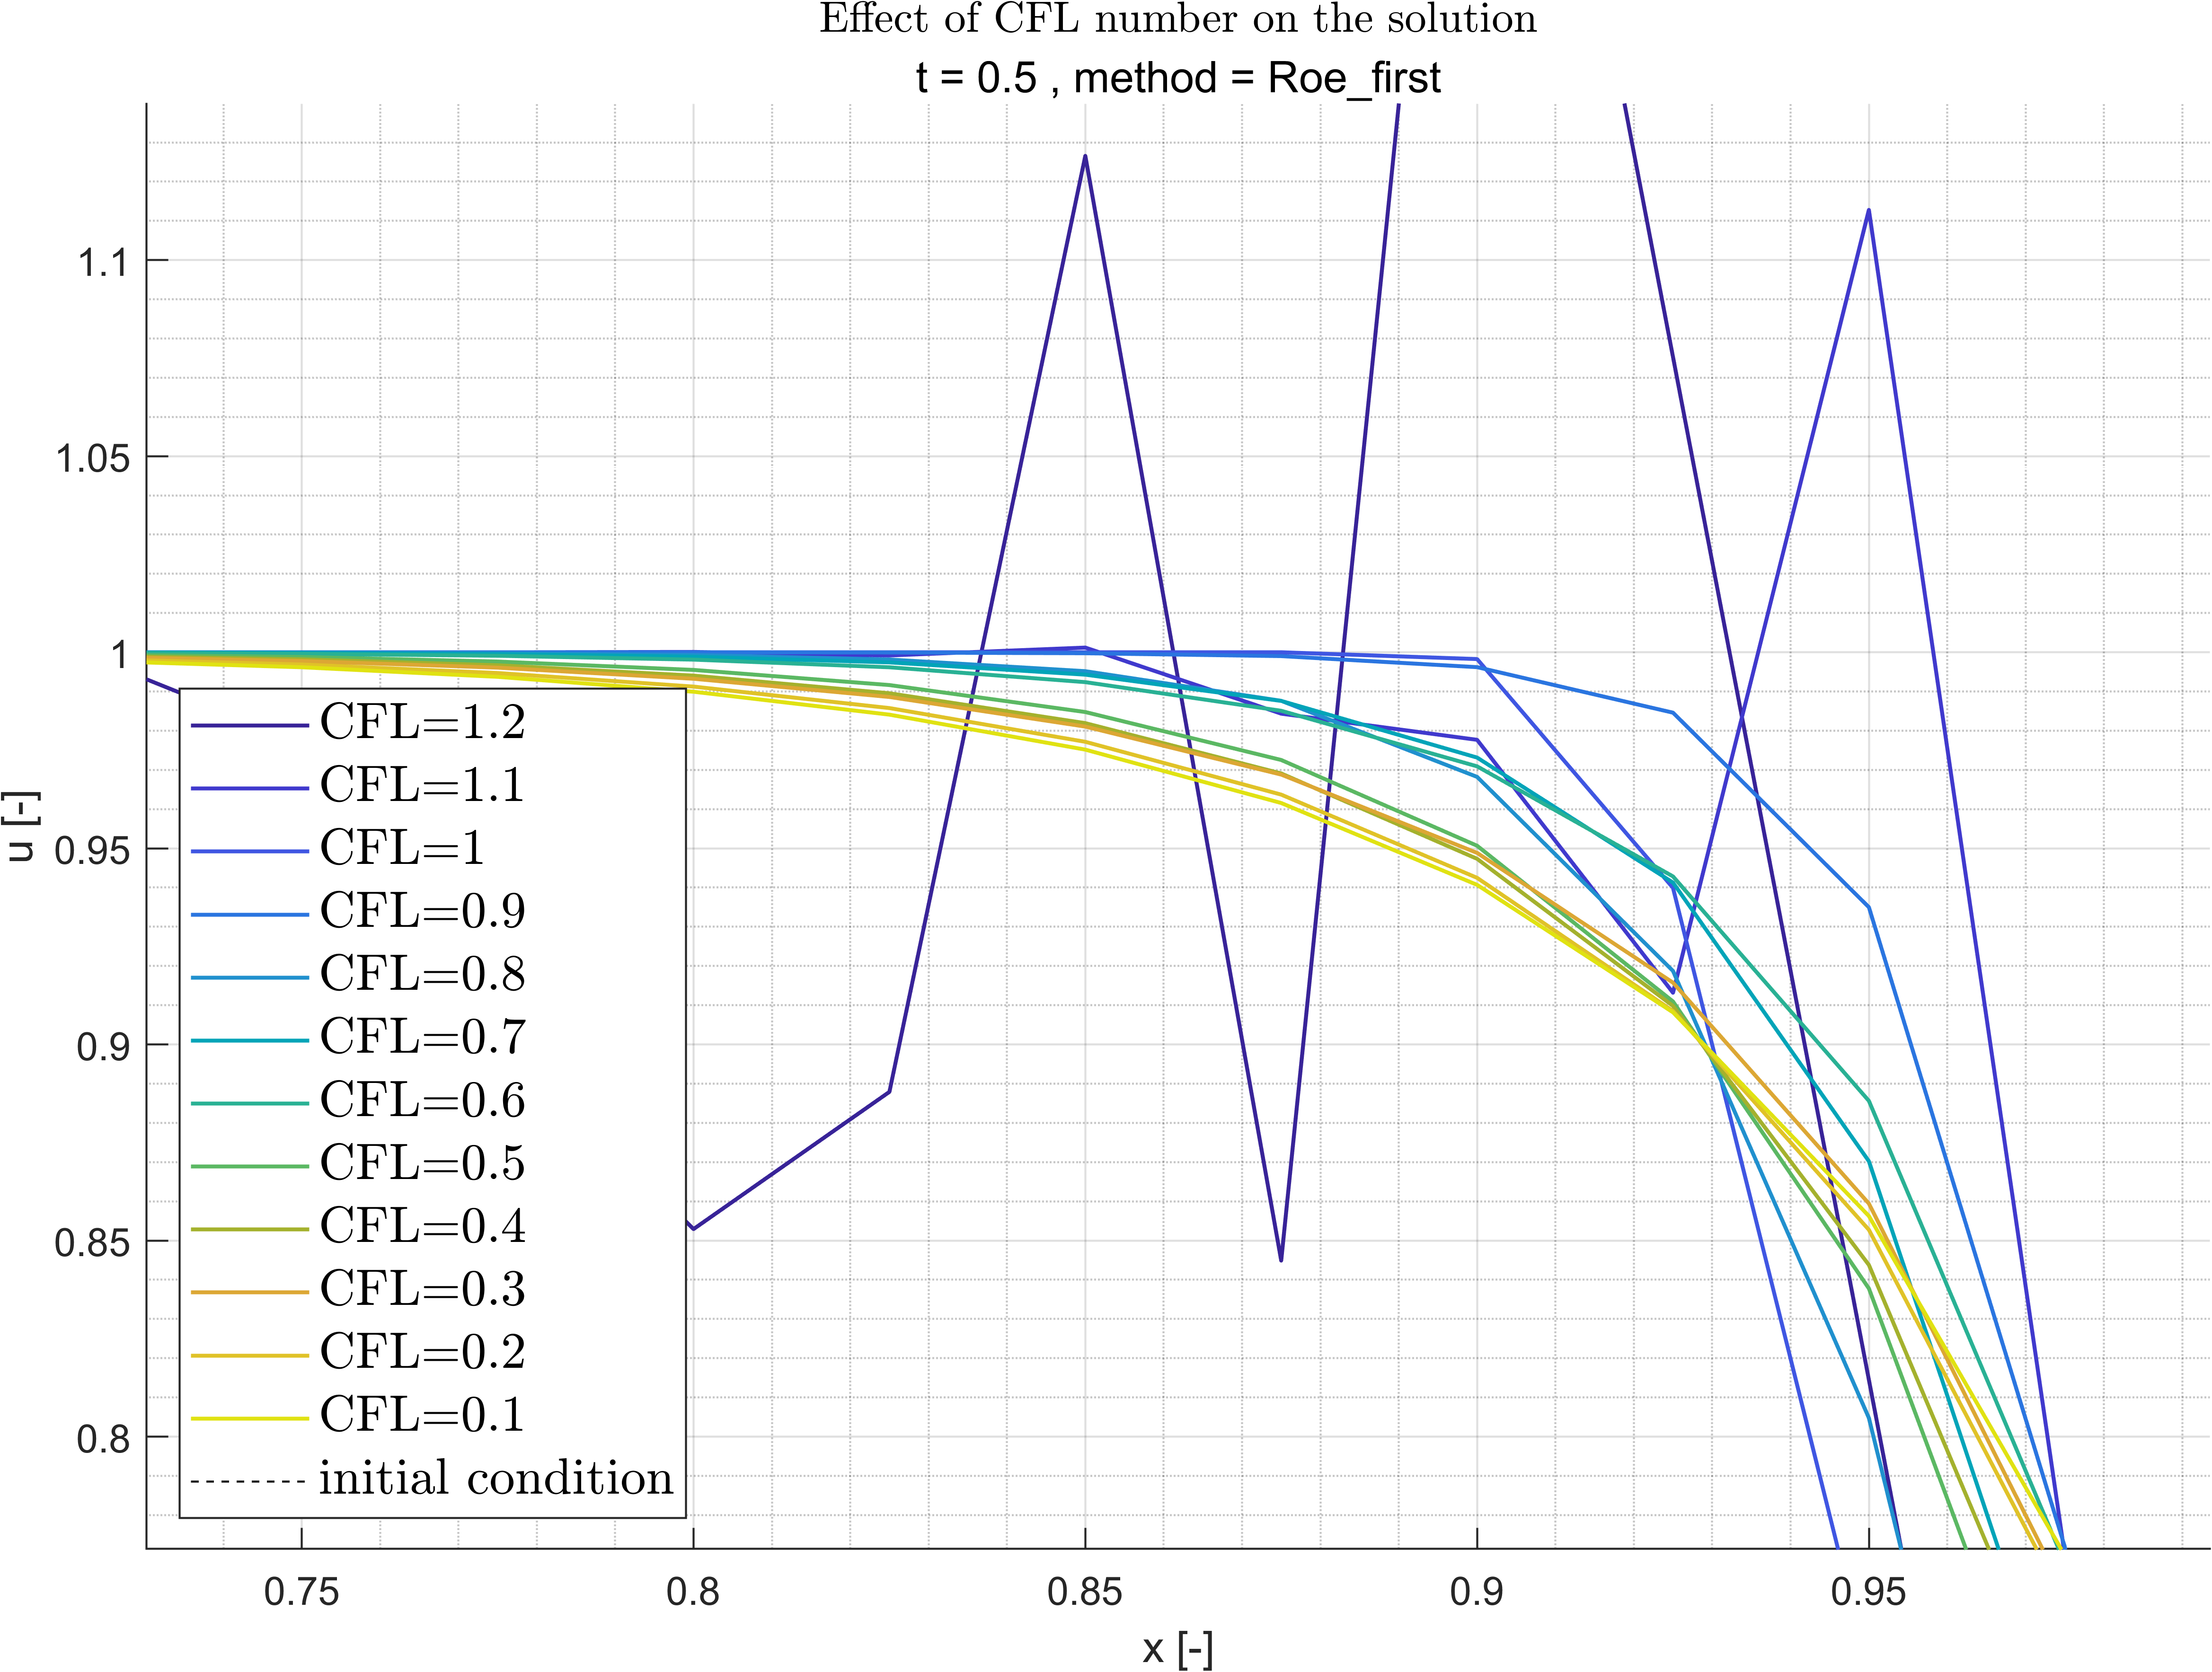
\includegraphics[width=\textwidth]{images/grap1.1.png}
        \caption{zoomed}
        \label{fig:roe_first_inviscid_B}
    \end{subfigure}
    \caption{Effect of CFL number on solution - Roe first order - inviscid}
    \label{fig:roe_first_inviscid}
\end{figure}
We can see that for CFL number bigger than 1, the solution becomes non-monotonic. As the CFL number increases, the solution becomes sharper near the wave.

\subsection{Second Order Roe $(u_1 = 0.5)$}
The first-order accurate Roe method interface flux function will be denoted like this:
\begin{equation*}
    f_{i+\frac{1}{2}}^{\mathrm{Roe},1}=f_{\left(u_i, u_{i+1}\right)}
\end{equation*}
The second order accurate Roe takes the form:
\begin{equation*}
    f_{i+\frac{1}{2}}^{\mathrm{Roe},2}=f_{\left(u_{i+1}^l, u_{i+1}^r\right)}
\end{equation*}
Hence:
\begin{equation}
    \begin{matrix}
        \displaystyle f_{i+\frac{1}{2}}^{\mathrm{Roe},2}=\frac{1}{2}\left(F_{\left(u_{1+\frac{1}{2}}^l\right)}+F_{\left(u_{1+\frac{1}{2}}^r\right)}-\left|\bar{u}_{i+\frac{1}{2}}\right|\left(u_{1+\frac{1}{2}}^r-u_{1+\frac{1}{2}}^l\right)\right) \\\\
        \displaystyle \bar{u}_{1+\frac{1}{2}}=\frac{F_{\left(u_{1+\frac{1}{2}}^r\right)}-F_{\left(u_{1+\frac{1}{2}}^l\right)}}{u_{1+\frac{1}{2}}^r-u_{1+\frac{1}{2}}^l} = \frac{u_{i+\frac{1}{2}}^l+u_{i+\frac{1}{2}}^r}{2}
    \end{matrix}
\end{equation}

\subsubsection{Without Limiters}
The interface values without limiters are evaluated as:
\begin{equation}
    \begin{matrix}
        \left\{\begin{array}{lcl}
            u_{i+\frac{1}{2}}^l & = & \displaystyle u_i+\frac{1-k}{4}\delta u_{i-\frac{1}{2}}+\frac{1+k}{4}\delta u_{i+\frac{1}{2}} \\\\
            u_{i+\frac{1}{2}}^r & = & \displaystyle u_{i+1}-\frac{1+k}{4}\delta u_{i+\frac{1}{2}}-\frac{1-k}{4}\delta u_{i+\frac{3}{2}}
        \end{array}\right. && \delta u_i\triangleq u_{i+\frac{1}{2}} - u_{i-\frac{1}{2}}
    \end{matrix}
\end{equation}
The parameter \emph{k} determines the scheme:
\begin{equation*}
    k = \left\{\begin{array}{cr}
        -1 & \mathrm{upwind} \\
        1 & \mathrm{central}
    \end{array}\right.
\end{equation*}

\subsubsection{With Limiters}
The interface values with limiters are evaluated as:
\begin{equation}
    \begin{matrix}
        \left\{\begin{array}{lcl}
            u_{i+\frac{1}{2}}^l & = & u_i+\frac{1-k}{4}\overline{\delta^+} u_{i-\frac{1}{2}}+\frac{1+k}{4}\overline{\delta^-} u_{i+\frac{1}{2}} \\
            u_{i+\frac{1}{2}}^r & = & u_{i+1}-\frac{1+k}{4}\overline{\delta^+} u_{i+\frac{1}{2}}-\frac{1-k}{4}\overline{\delta^-} u_{i+\frac{3}{2}}
        \end{array}\right. && {\overline{\delta^\pm}} u\text{ are limited slopes}
    \end{matrix}
\end{equation}
$\overline{\delta}$ is an operator such that $\overline{\delta}u_i=\psi\delta u_i$, where $\psi\left(r\right)$ is a limiter function and:
\begin{equation}
    r^\pm=\left\{\begin{array}{ccc}
        r_{1+\frac{1}{2}}^+ & \triangleq & \displaystyle\frac{u_{i+2}-u_{i+1}}{u_{i+1}-u_i}=\frac{\Delta u_{i+1}}{\Delta u_i} \\
        r_{1+\frac{1}{2}}^- & \triangleq & \displaystyle\frac{u_{i}-u_{i-1}}{u_{i+1}-u_i}=\frac{\nabla u_{i}}{\nabla u_{i+1}}
    \end{array}\right.
\end{equation}
There are many types of limiters. For example:
\begin{itemize}
    \item van Albada $$\psi\left(r\right)=\frac{r+r^2}{1+r^2}$$
    \item van Leer $$\psi\left(r\right)=\frac{r+\left|r\right|}{1+r^2}$$
    \item minmod$(x,y)$ $$\psi\left(r\right)=\left\{\begin{array}{ccccc}
        x & \mathrm{if} & \left|x\right|<\left|y\right| & \mathrm{and} & xy>0 \\
        y & \mathrm{if} & \left|x\right|>\left|y\right| & \mathrm{and} & xy>0 \\
        0 & \mathrm{if} & & & xy<0 
    \end{array}\right.$$
    \item Superbee(Roe) $$\psi\left(r\right)=\max\left(0,\min\left(2r,1\right),\min\left(r,2\right)\right)$$

\end{itemize}

\subsubsection{Effect of CFL}
\begin{figure}[H]
    \centering
    \begin{subfigure}[c]{.49\textwidth}
        \centering
        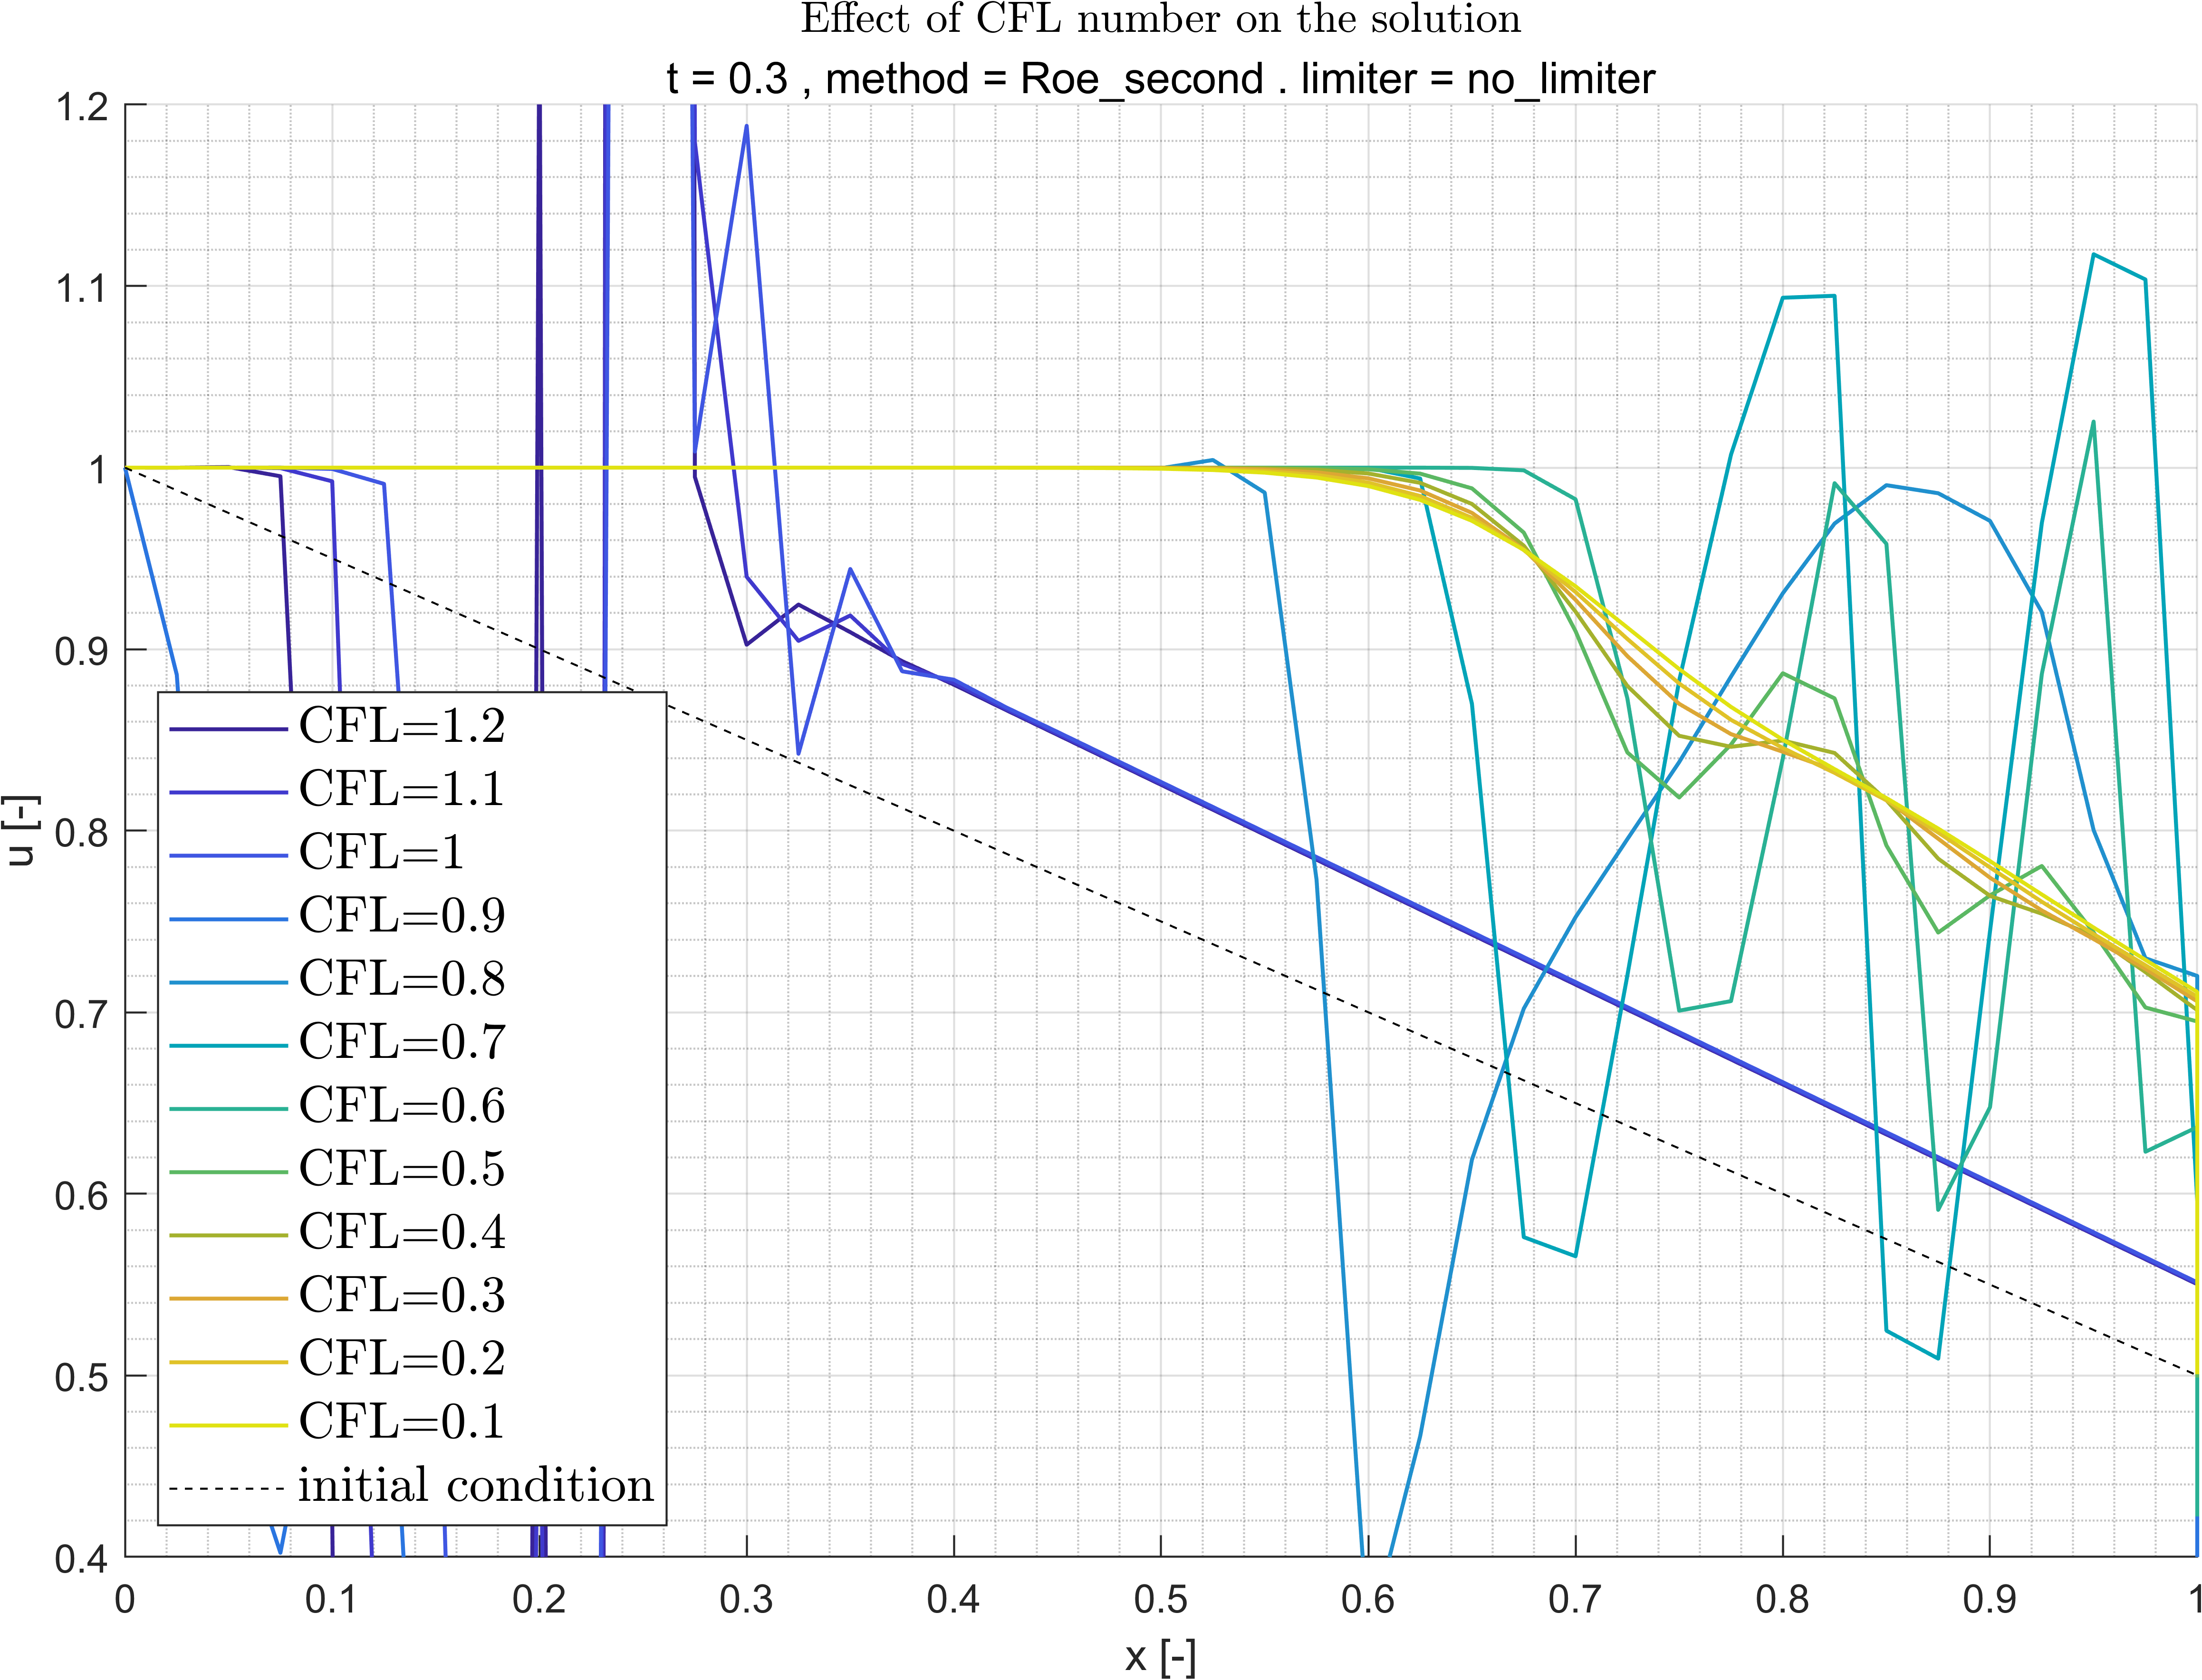
\includegraphics[width=\textwidth]{images/grap2.png}
        \caption{no limiters}
        \label{fig:roe_second_no_limiter_A}
    \end{subfigure}
    \hfill
    \begin{subfigure}[c]{.49\textwidth}
        \centering
        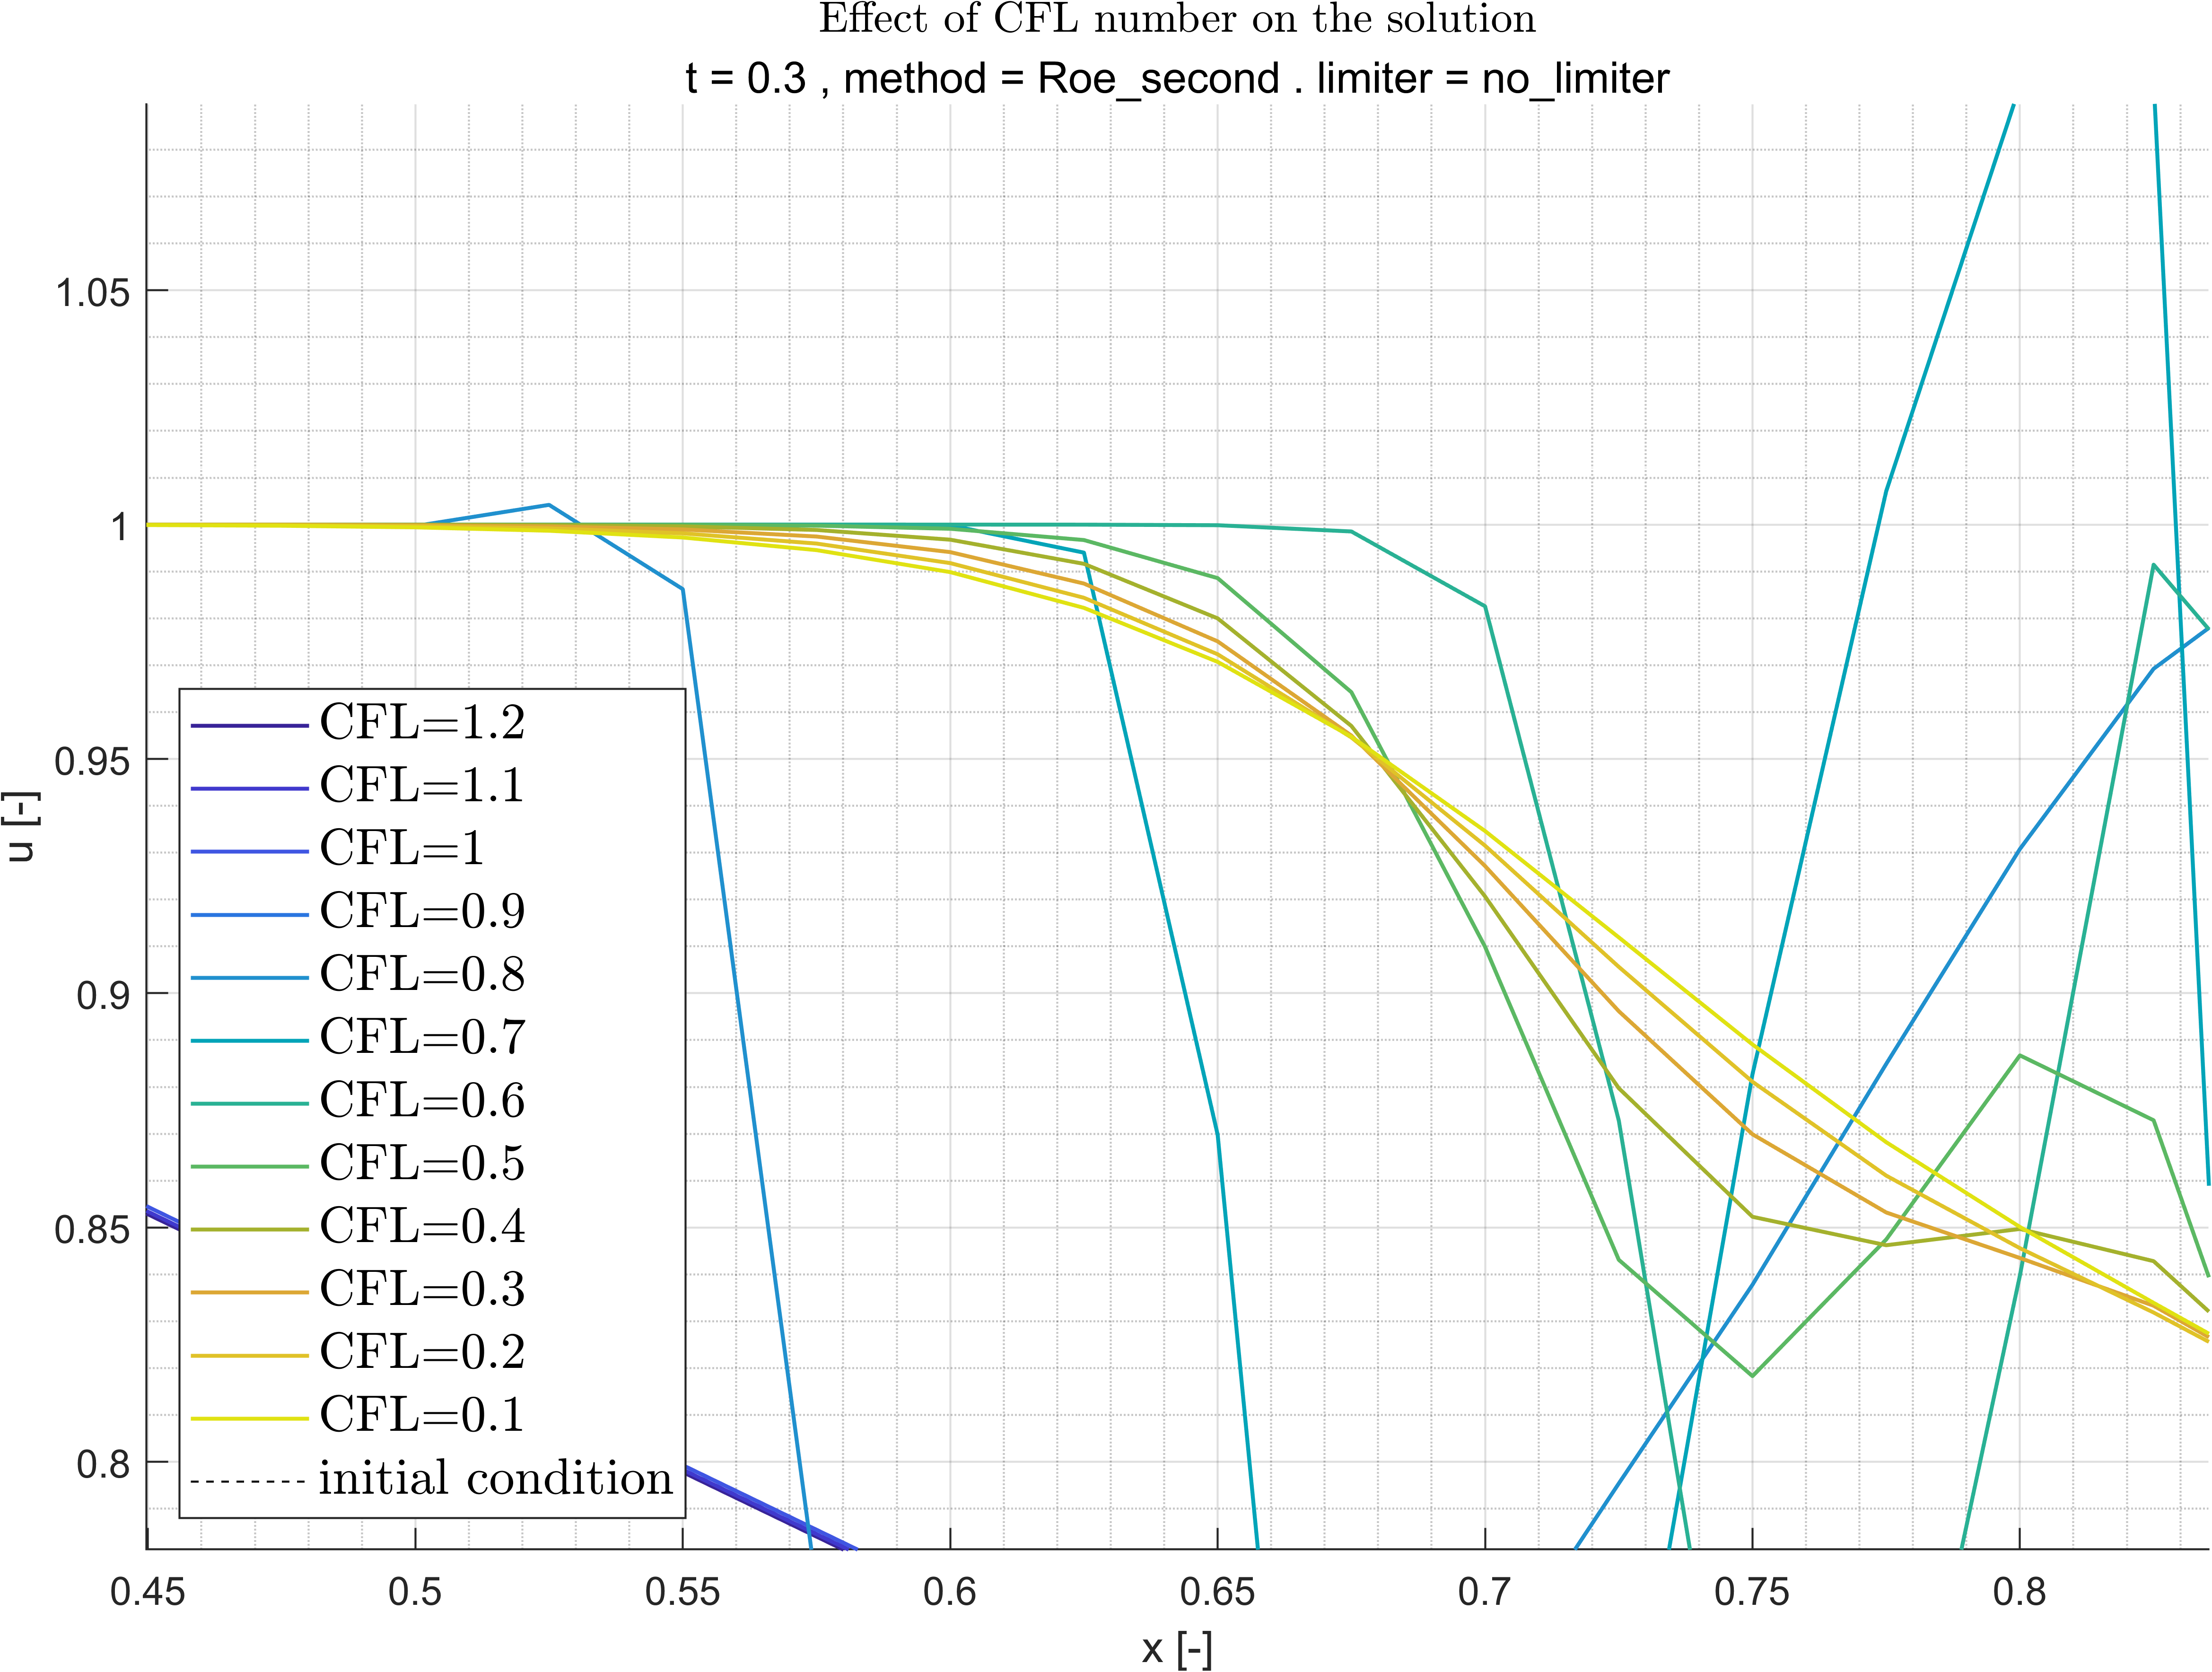
\includegraphics[width=\textwidth]{images/grap2.1.png}
        \caption{no limiters - zoomed}
        \label{fig:roe_second_no_limiter_B}
    \end{subfigure}
    \caption{Effect of CFL number on solution - Roe second order with no limiters}
    \label{fig:roe_second_no_limiter}
\end{figure}
\noindent We can see that when there are no limiters, for CFL number bigger than 0.8, the solution does not converge. As the CFL number increases, the oscillations increase. At low CFL numbers, the oscillations are not pronounced since the time step is really small.
\begin{figure}[H]
    \centering
    \begin{subfigure}[c]{.35\textwidth}
        \centering
        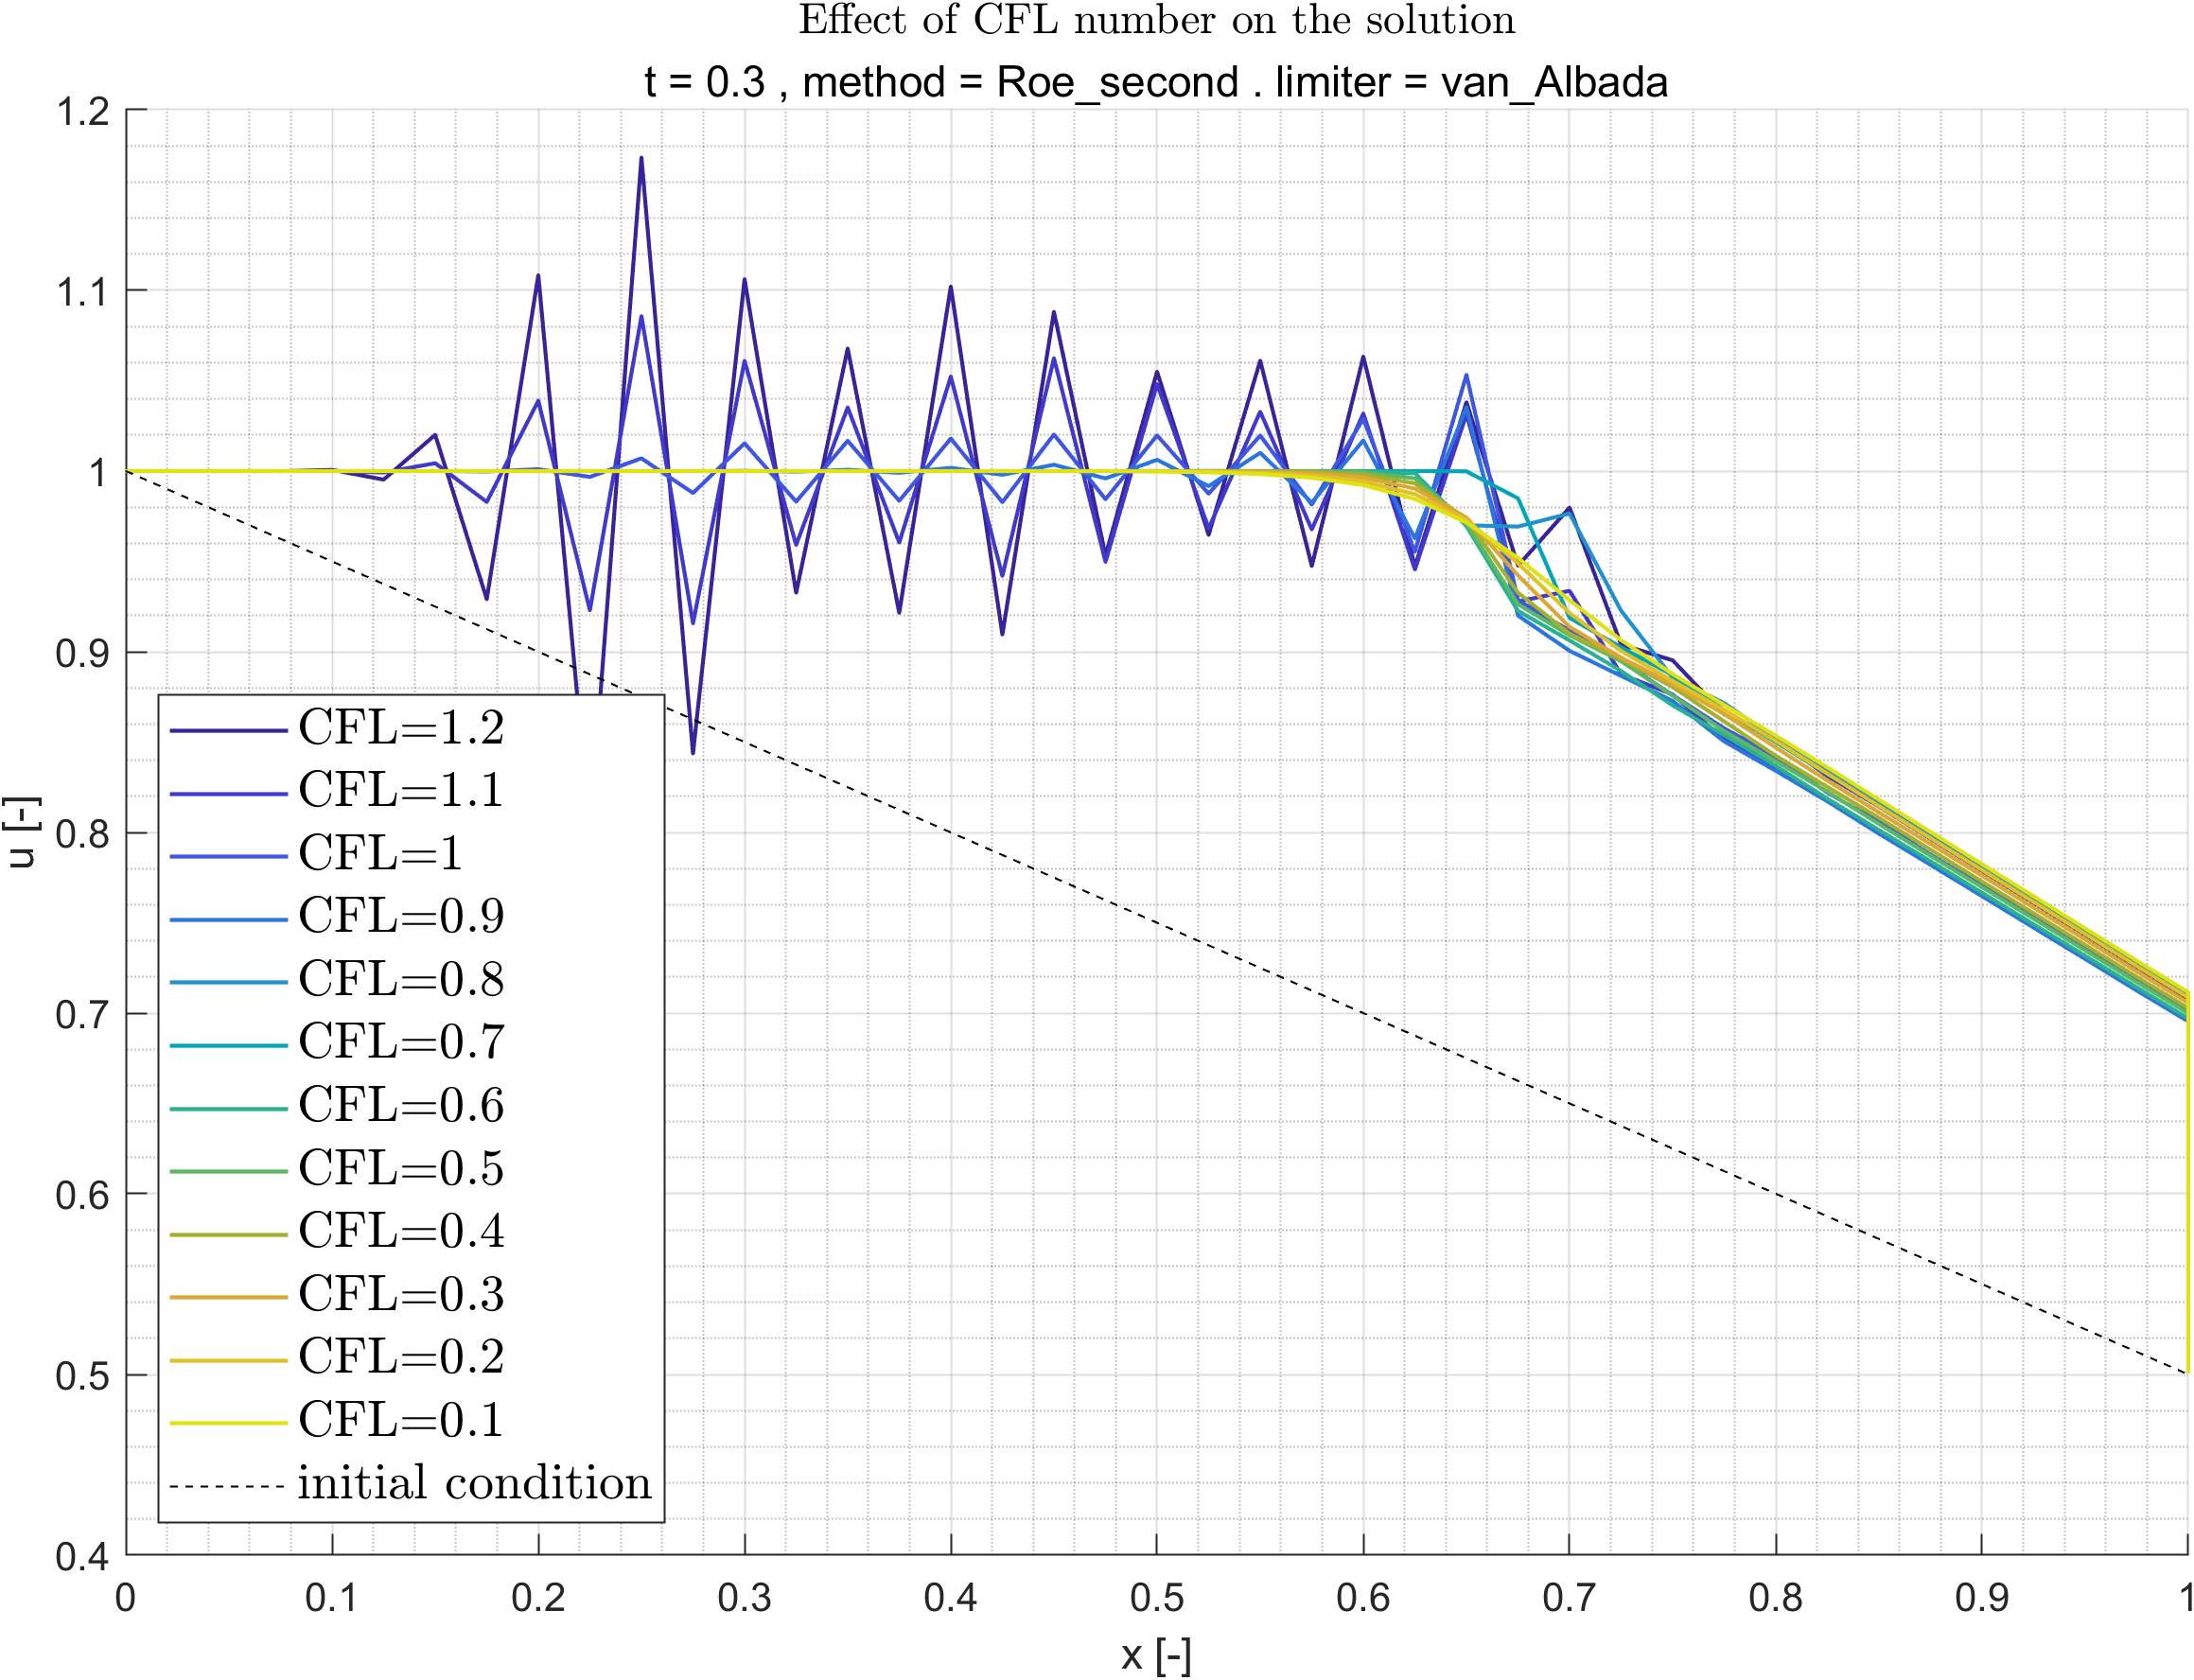
\includegraphics[width=\textwidth]{images/grap3.png}
        \caption{van Albada}
        \label{fig:roe_second_van_Albada_A}
    \end{subfigure}
    % \hfill
    \begin{subfigure}[c]{.35\textwidth}
        \centering
        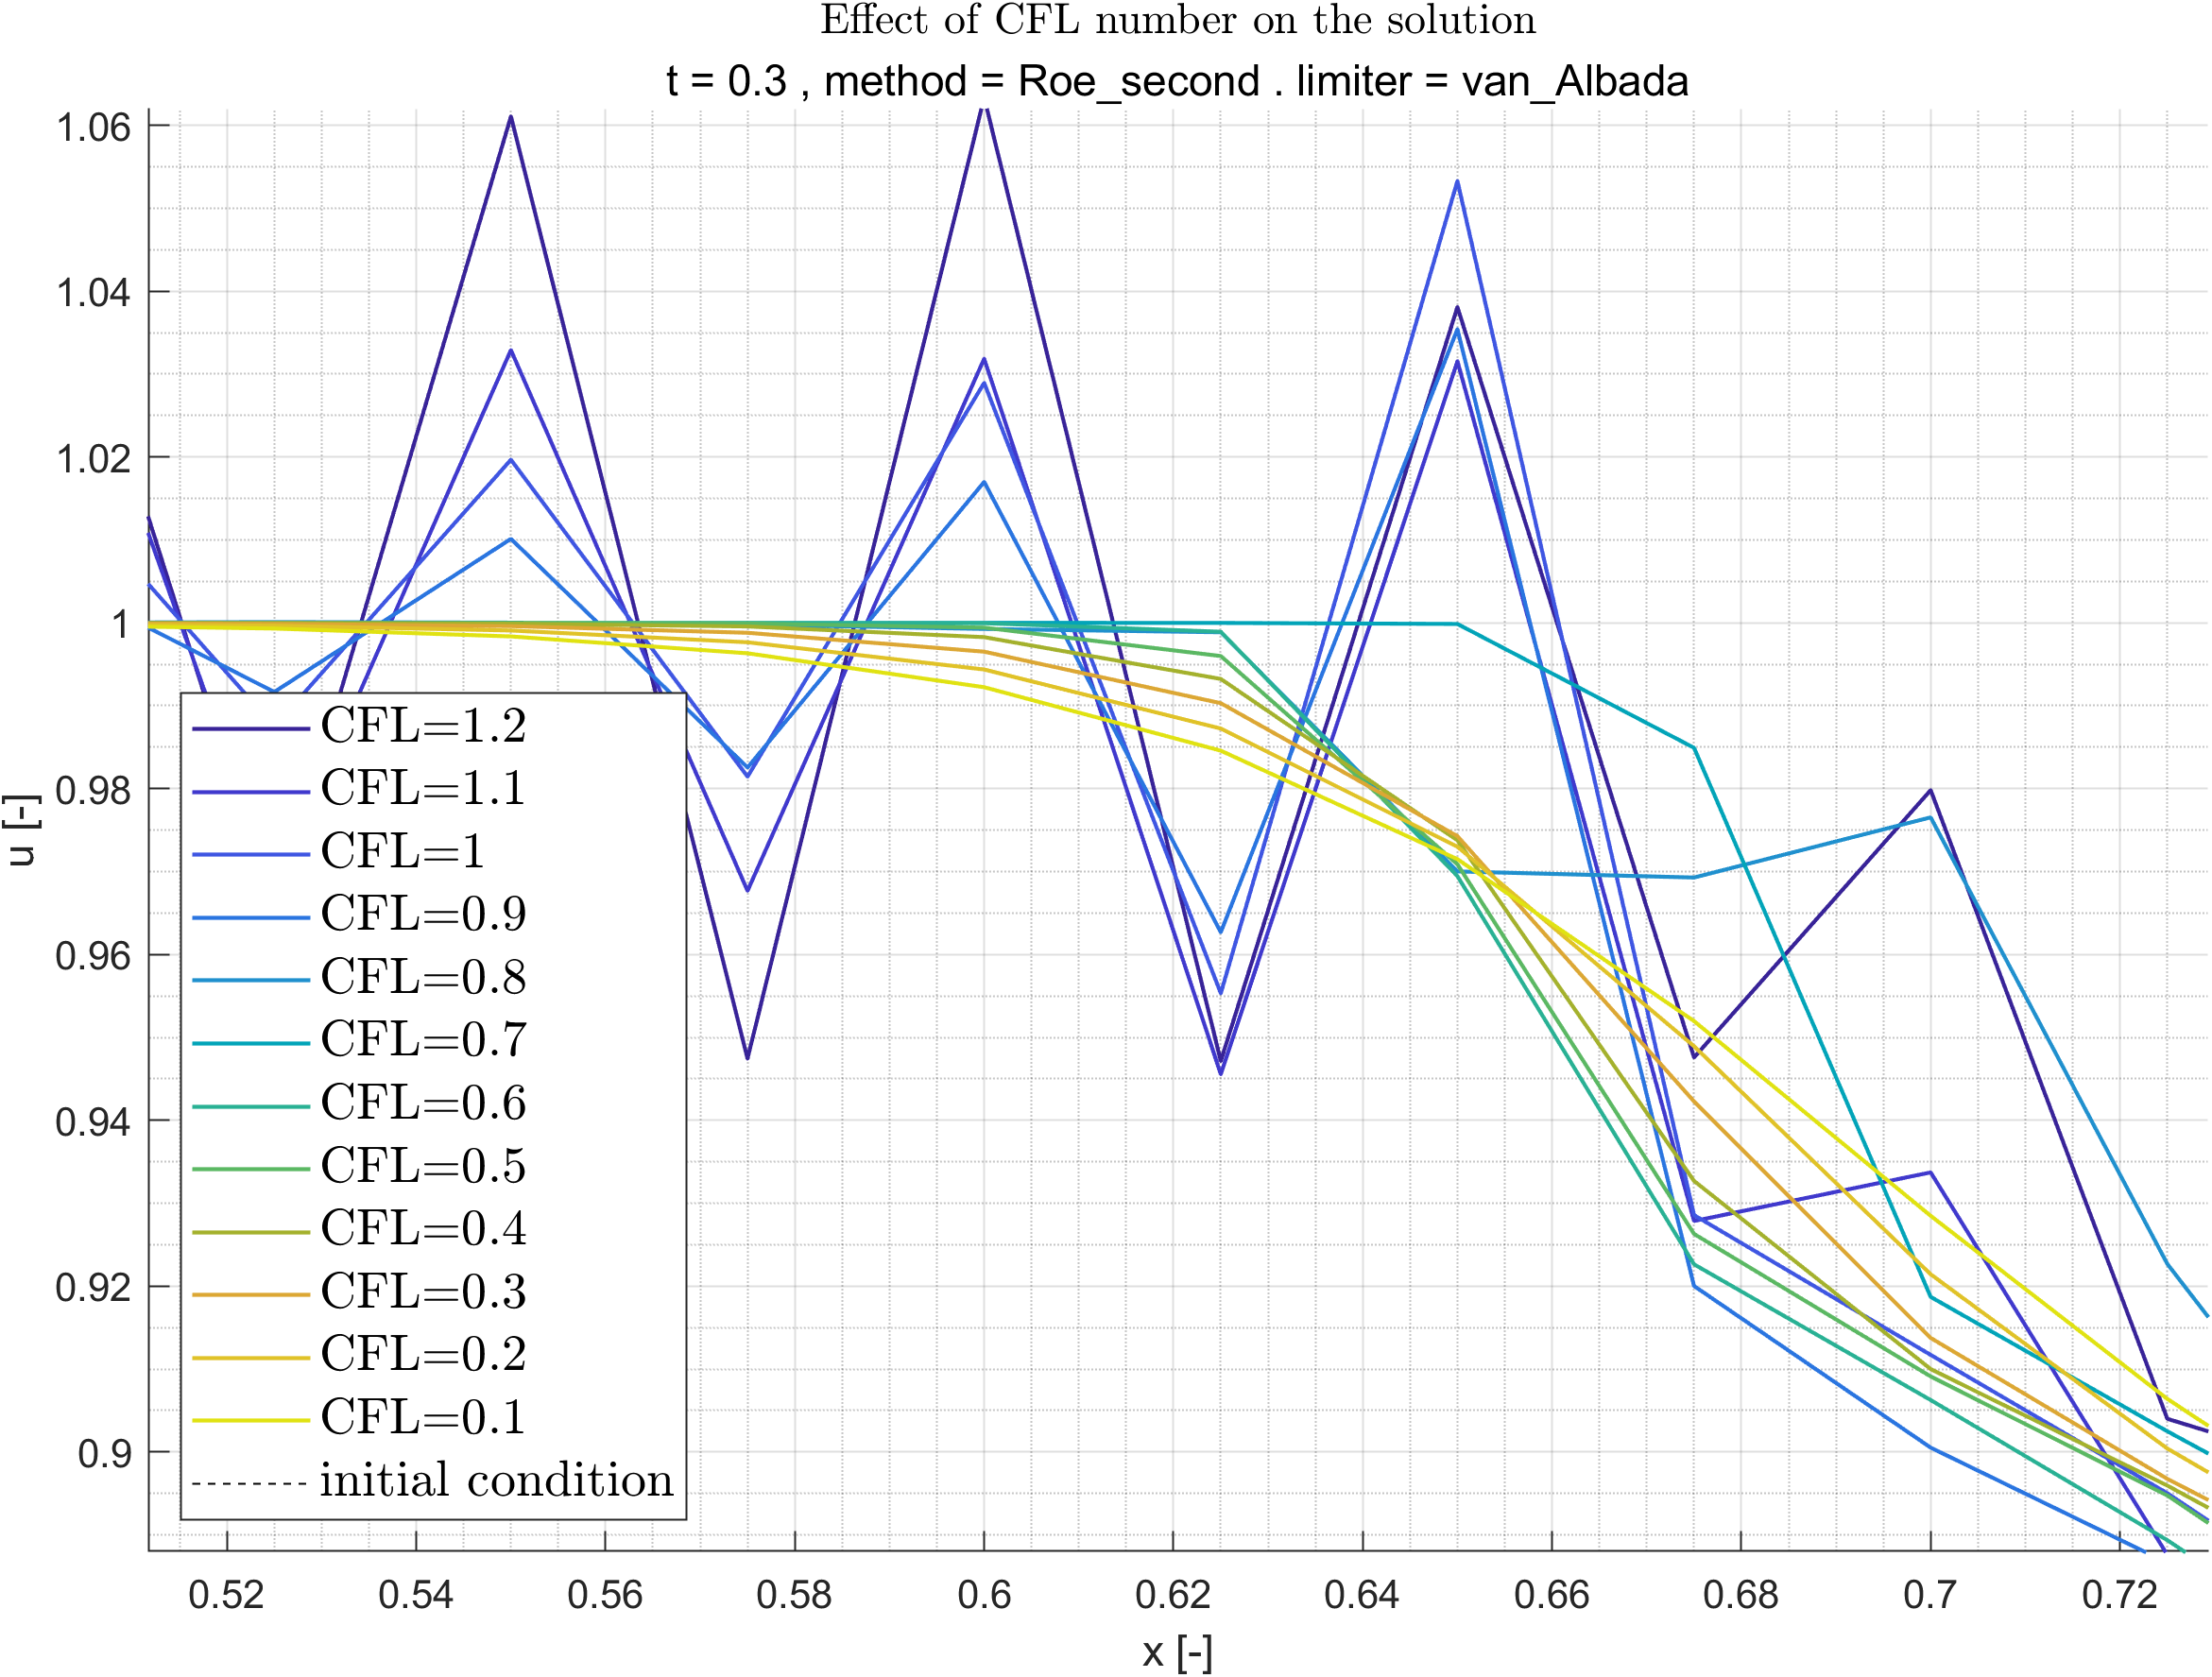
\includegraphics[width=\textwidth]{images/grap3.1.png}
        \caption{van Albada - zoomed}
        \label{fig:roe_second_van_Albada_B}
    \end{subfigure}
    \begin{subfigure}[c]{.35\textwidth}
        \centering
        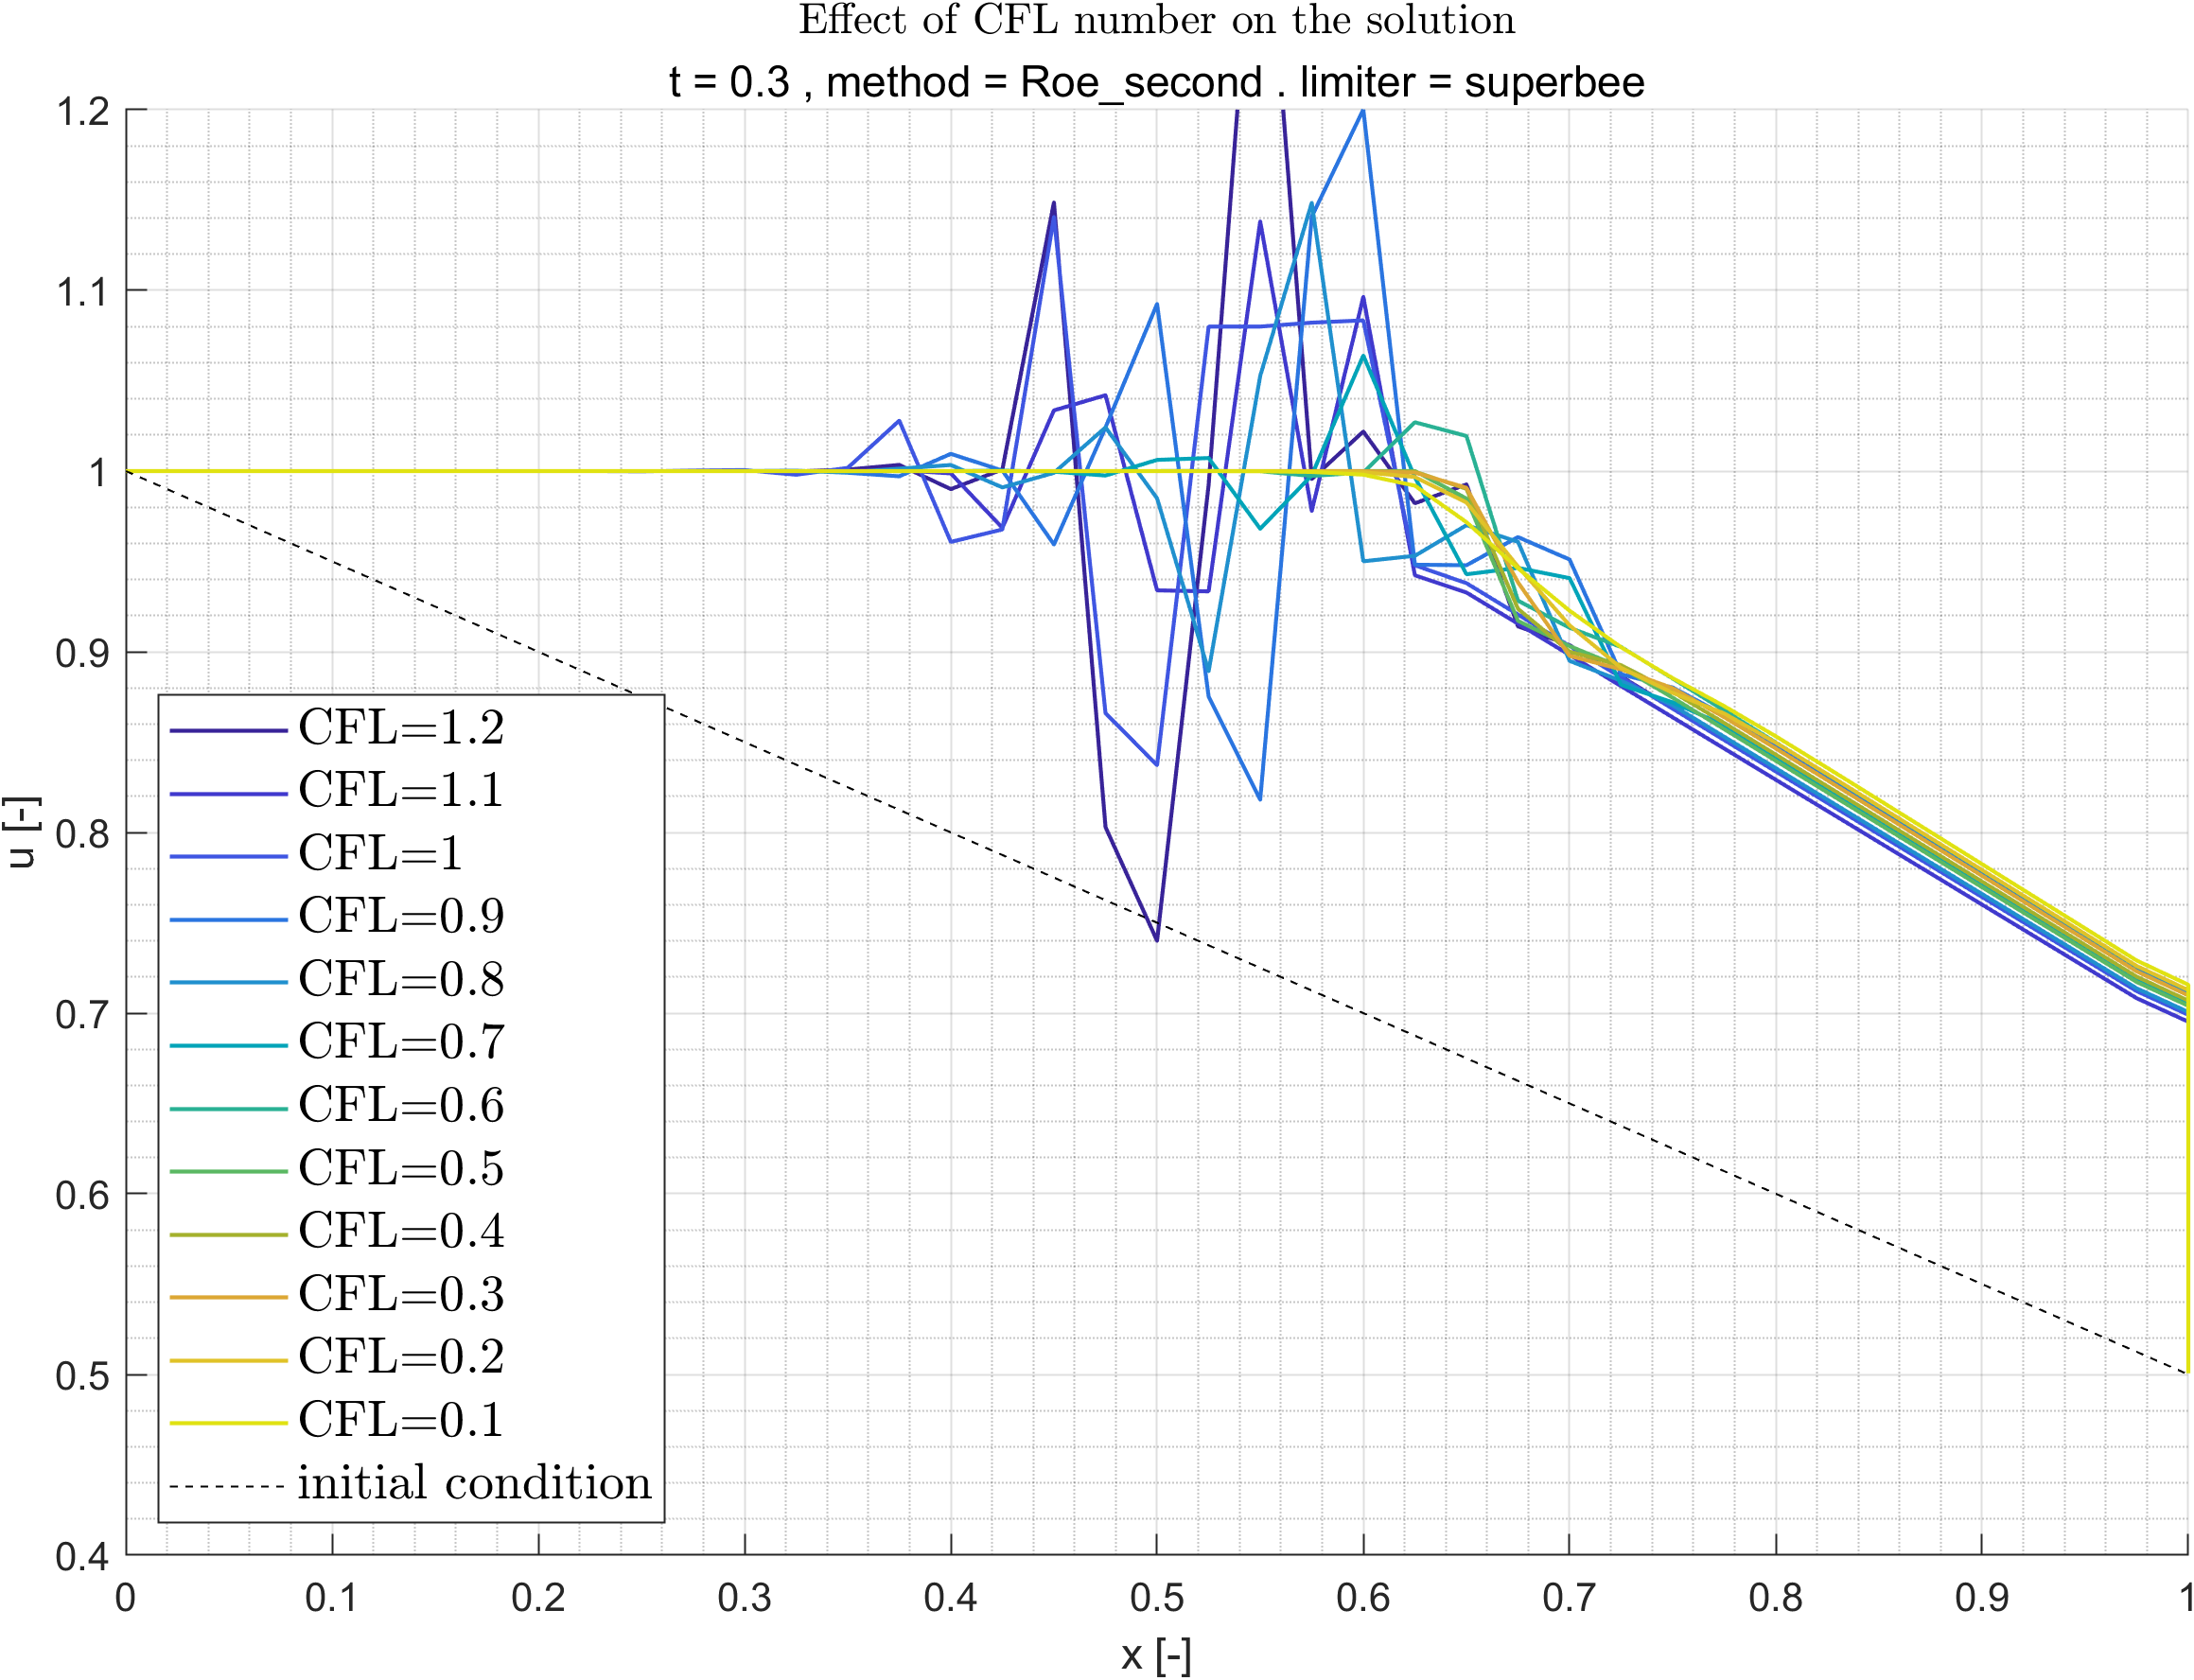
\includegraphics[width=\textwidth]{images/grap4.png}
        \caption{superbee}
        \label{fig:roe_second_superbee_A}
    \end{subfigure}
    % \hfill
    \begin{subfigure}[c]{.35\textwidth}
        \centering
        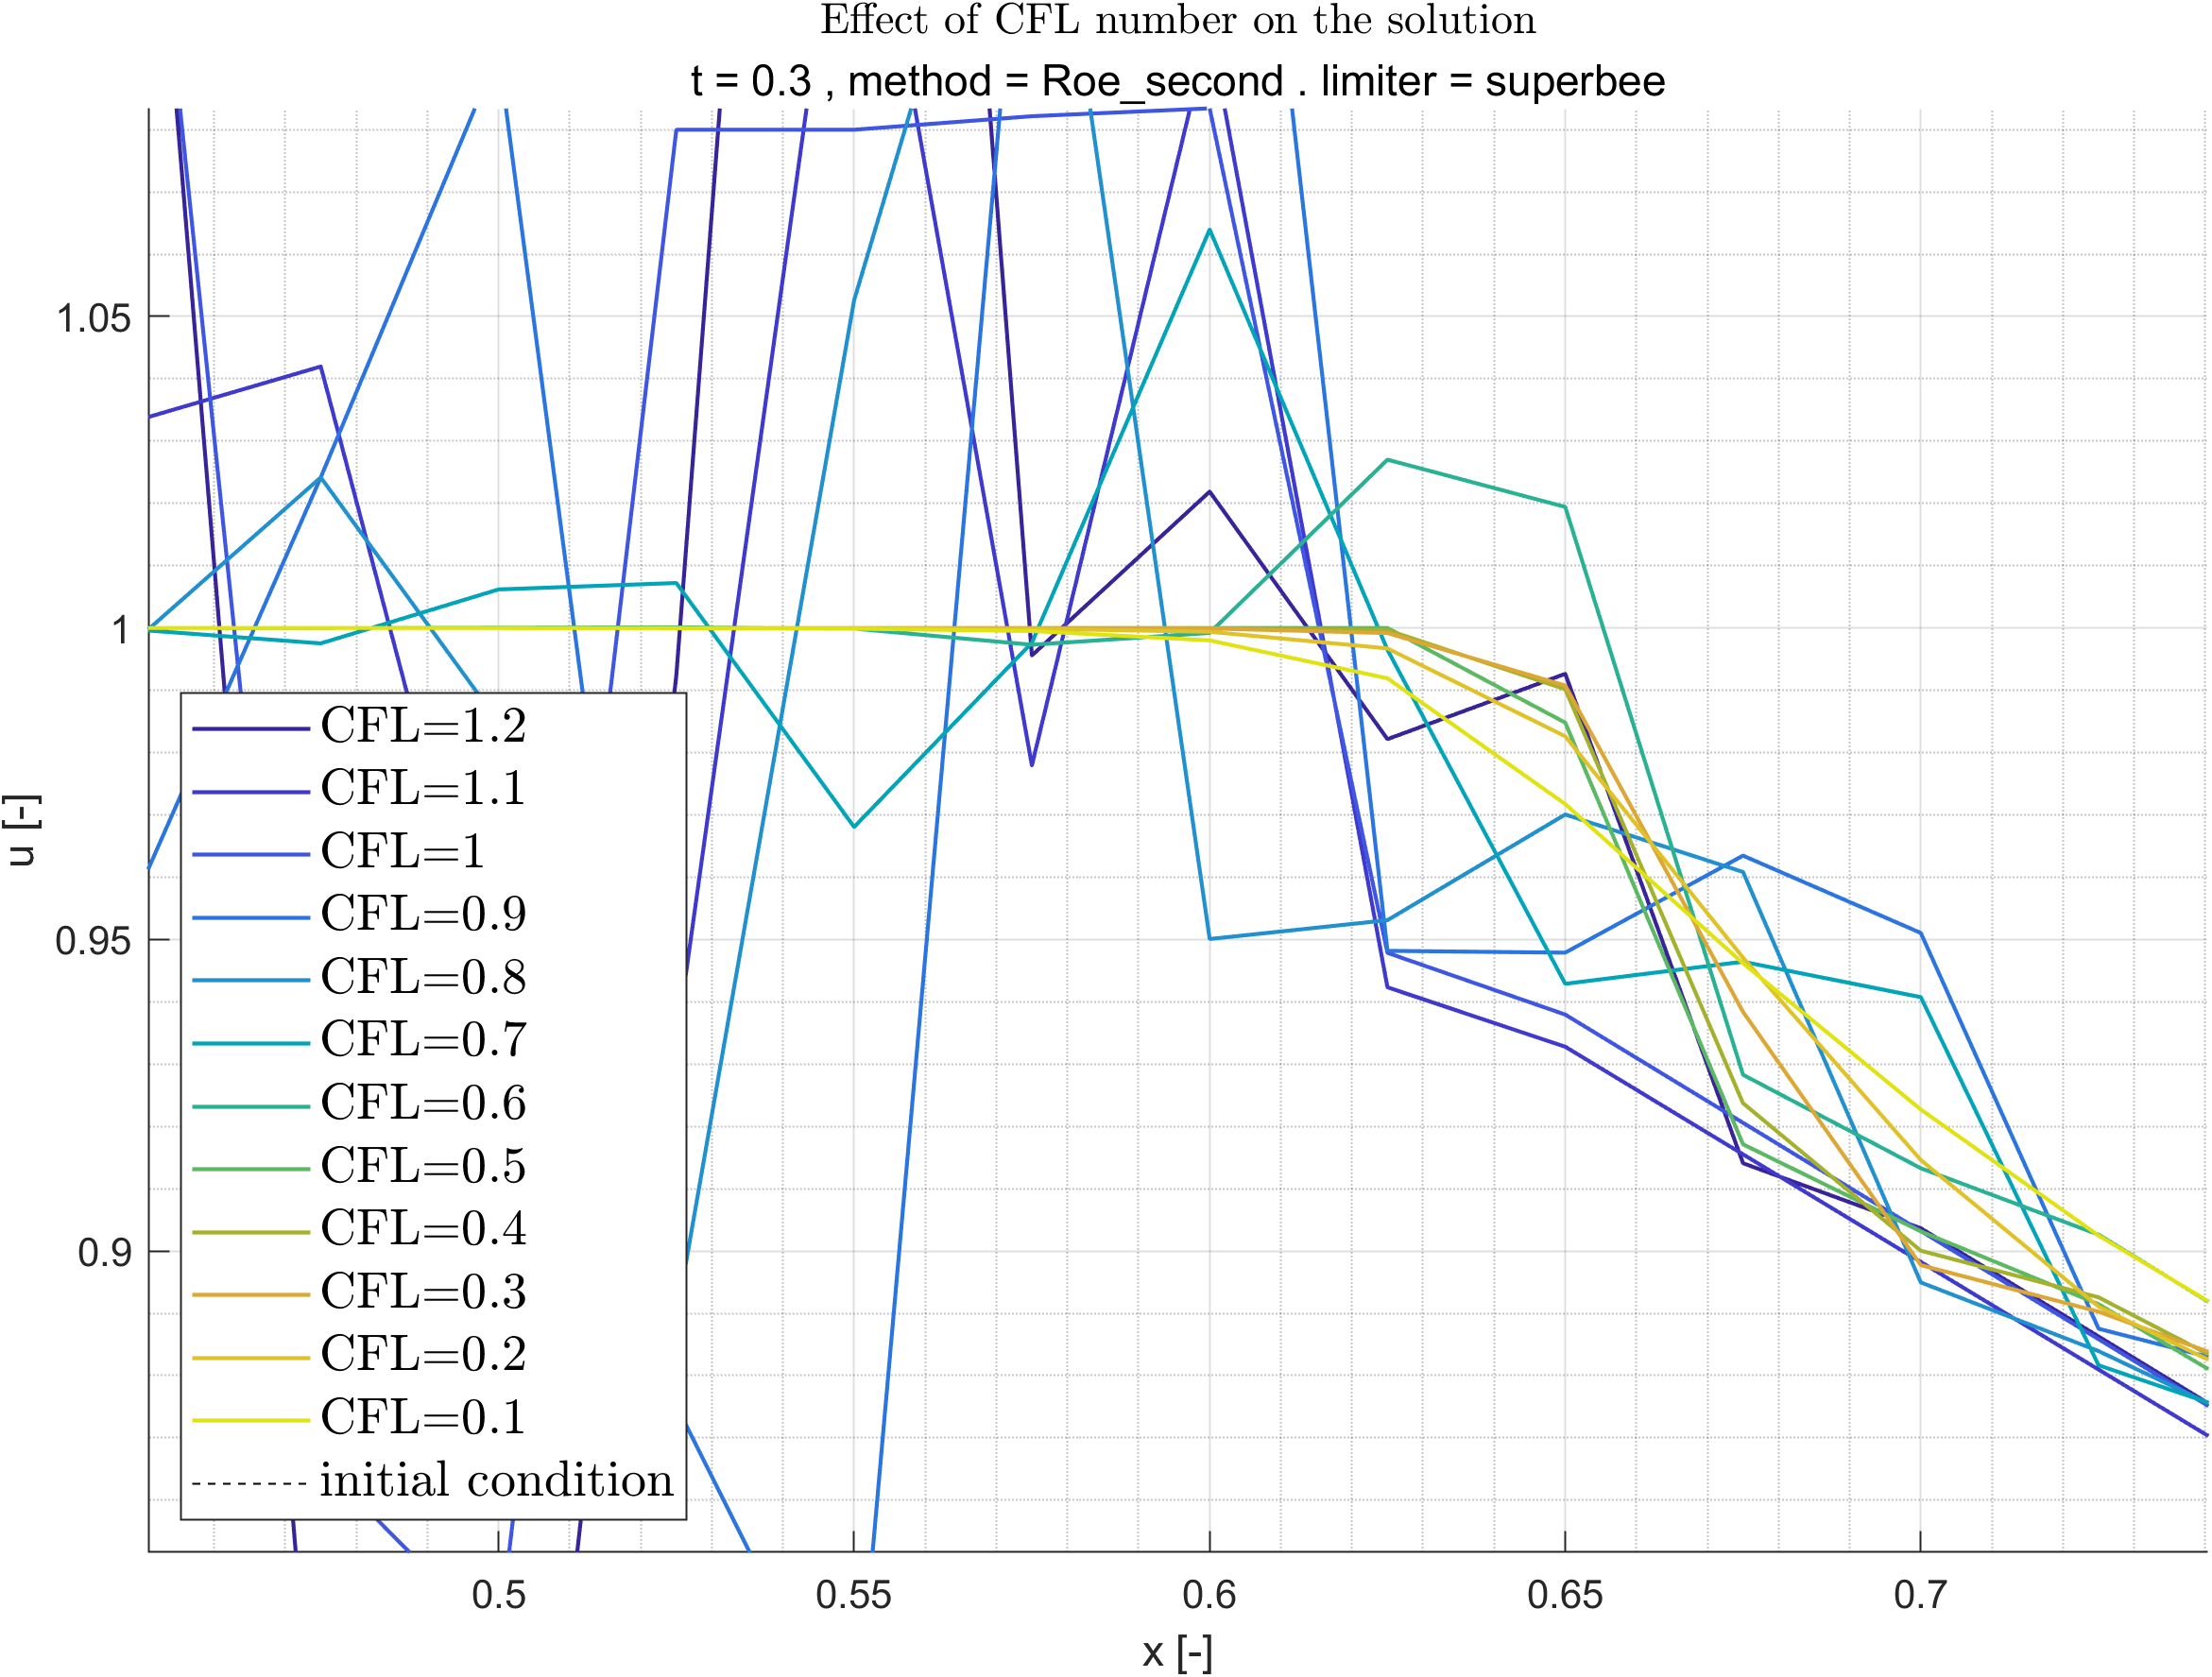
\includegraphics[width=\textwidth]{images/grap4.1.png}
        \caption{superbee - zoomed}
        \label{fig:roe_second_superbee_B}
    \end{subfigure}
    \begin{subfigure}[c]{.35\textwidth}
        \centering
        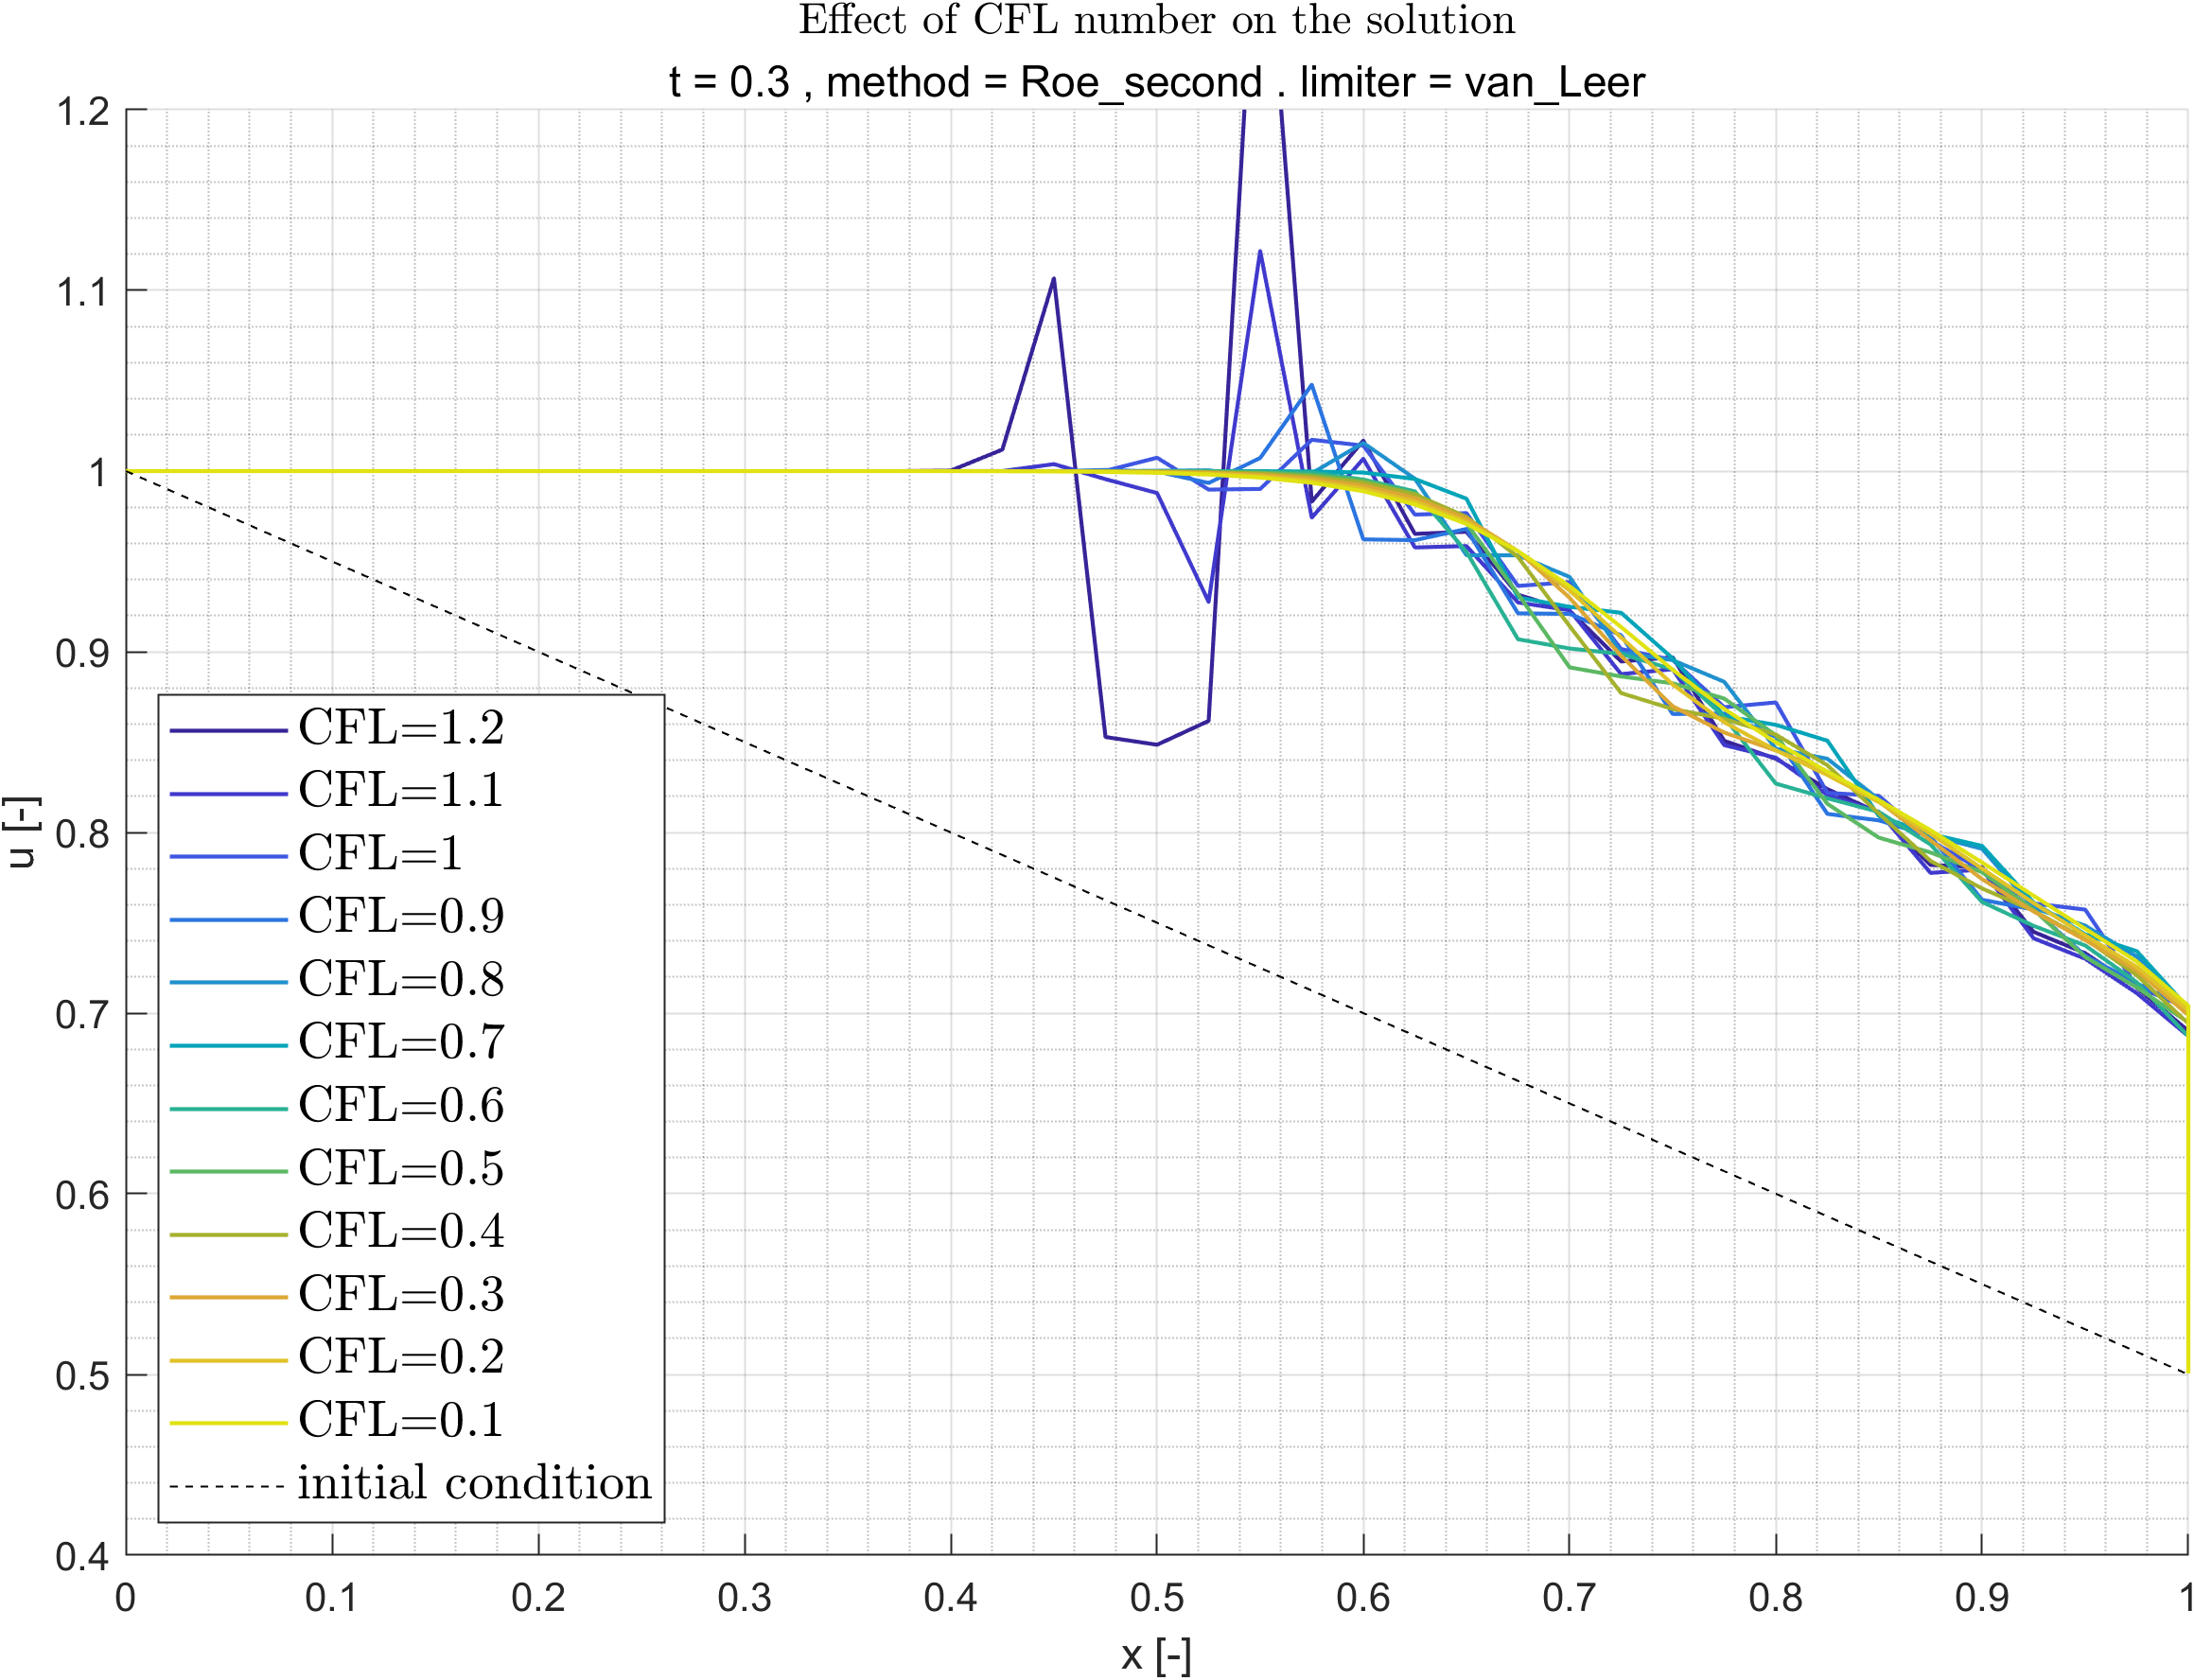
\includegraphics[width=\textwidth]{images/grap5.png}
        \caption{van Leer}
        \label{fig:roe_second_van_Leer_A}
    \end{subfigure}
    % \hfill
    \begin{subfigure}[c]{.35\textwidth}
        \centering
        \includegraphics[width=\textwidth]{images/grap5.1.png}
        \caption{van Leer - zoomed}
        \label{fig:roe_second_van_Leer_B}
    \end{subfigure}
    \begin{subfigure}[c]{.35\textwidth}
        \centering
        \includegraphics[width=\textwidth]{images/grap6.png}
        \caption{minmod}
        \label{fig:roe_second_minmod_A}
    \end{subfigure}
    % \hfill
    \begin{subfigure}[c]{.35\textwidth}
        \centering
        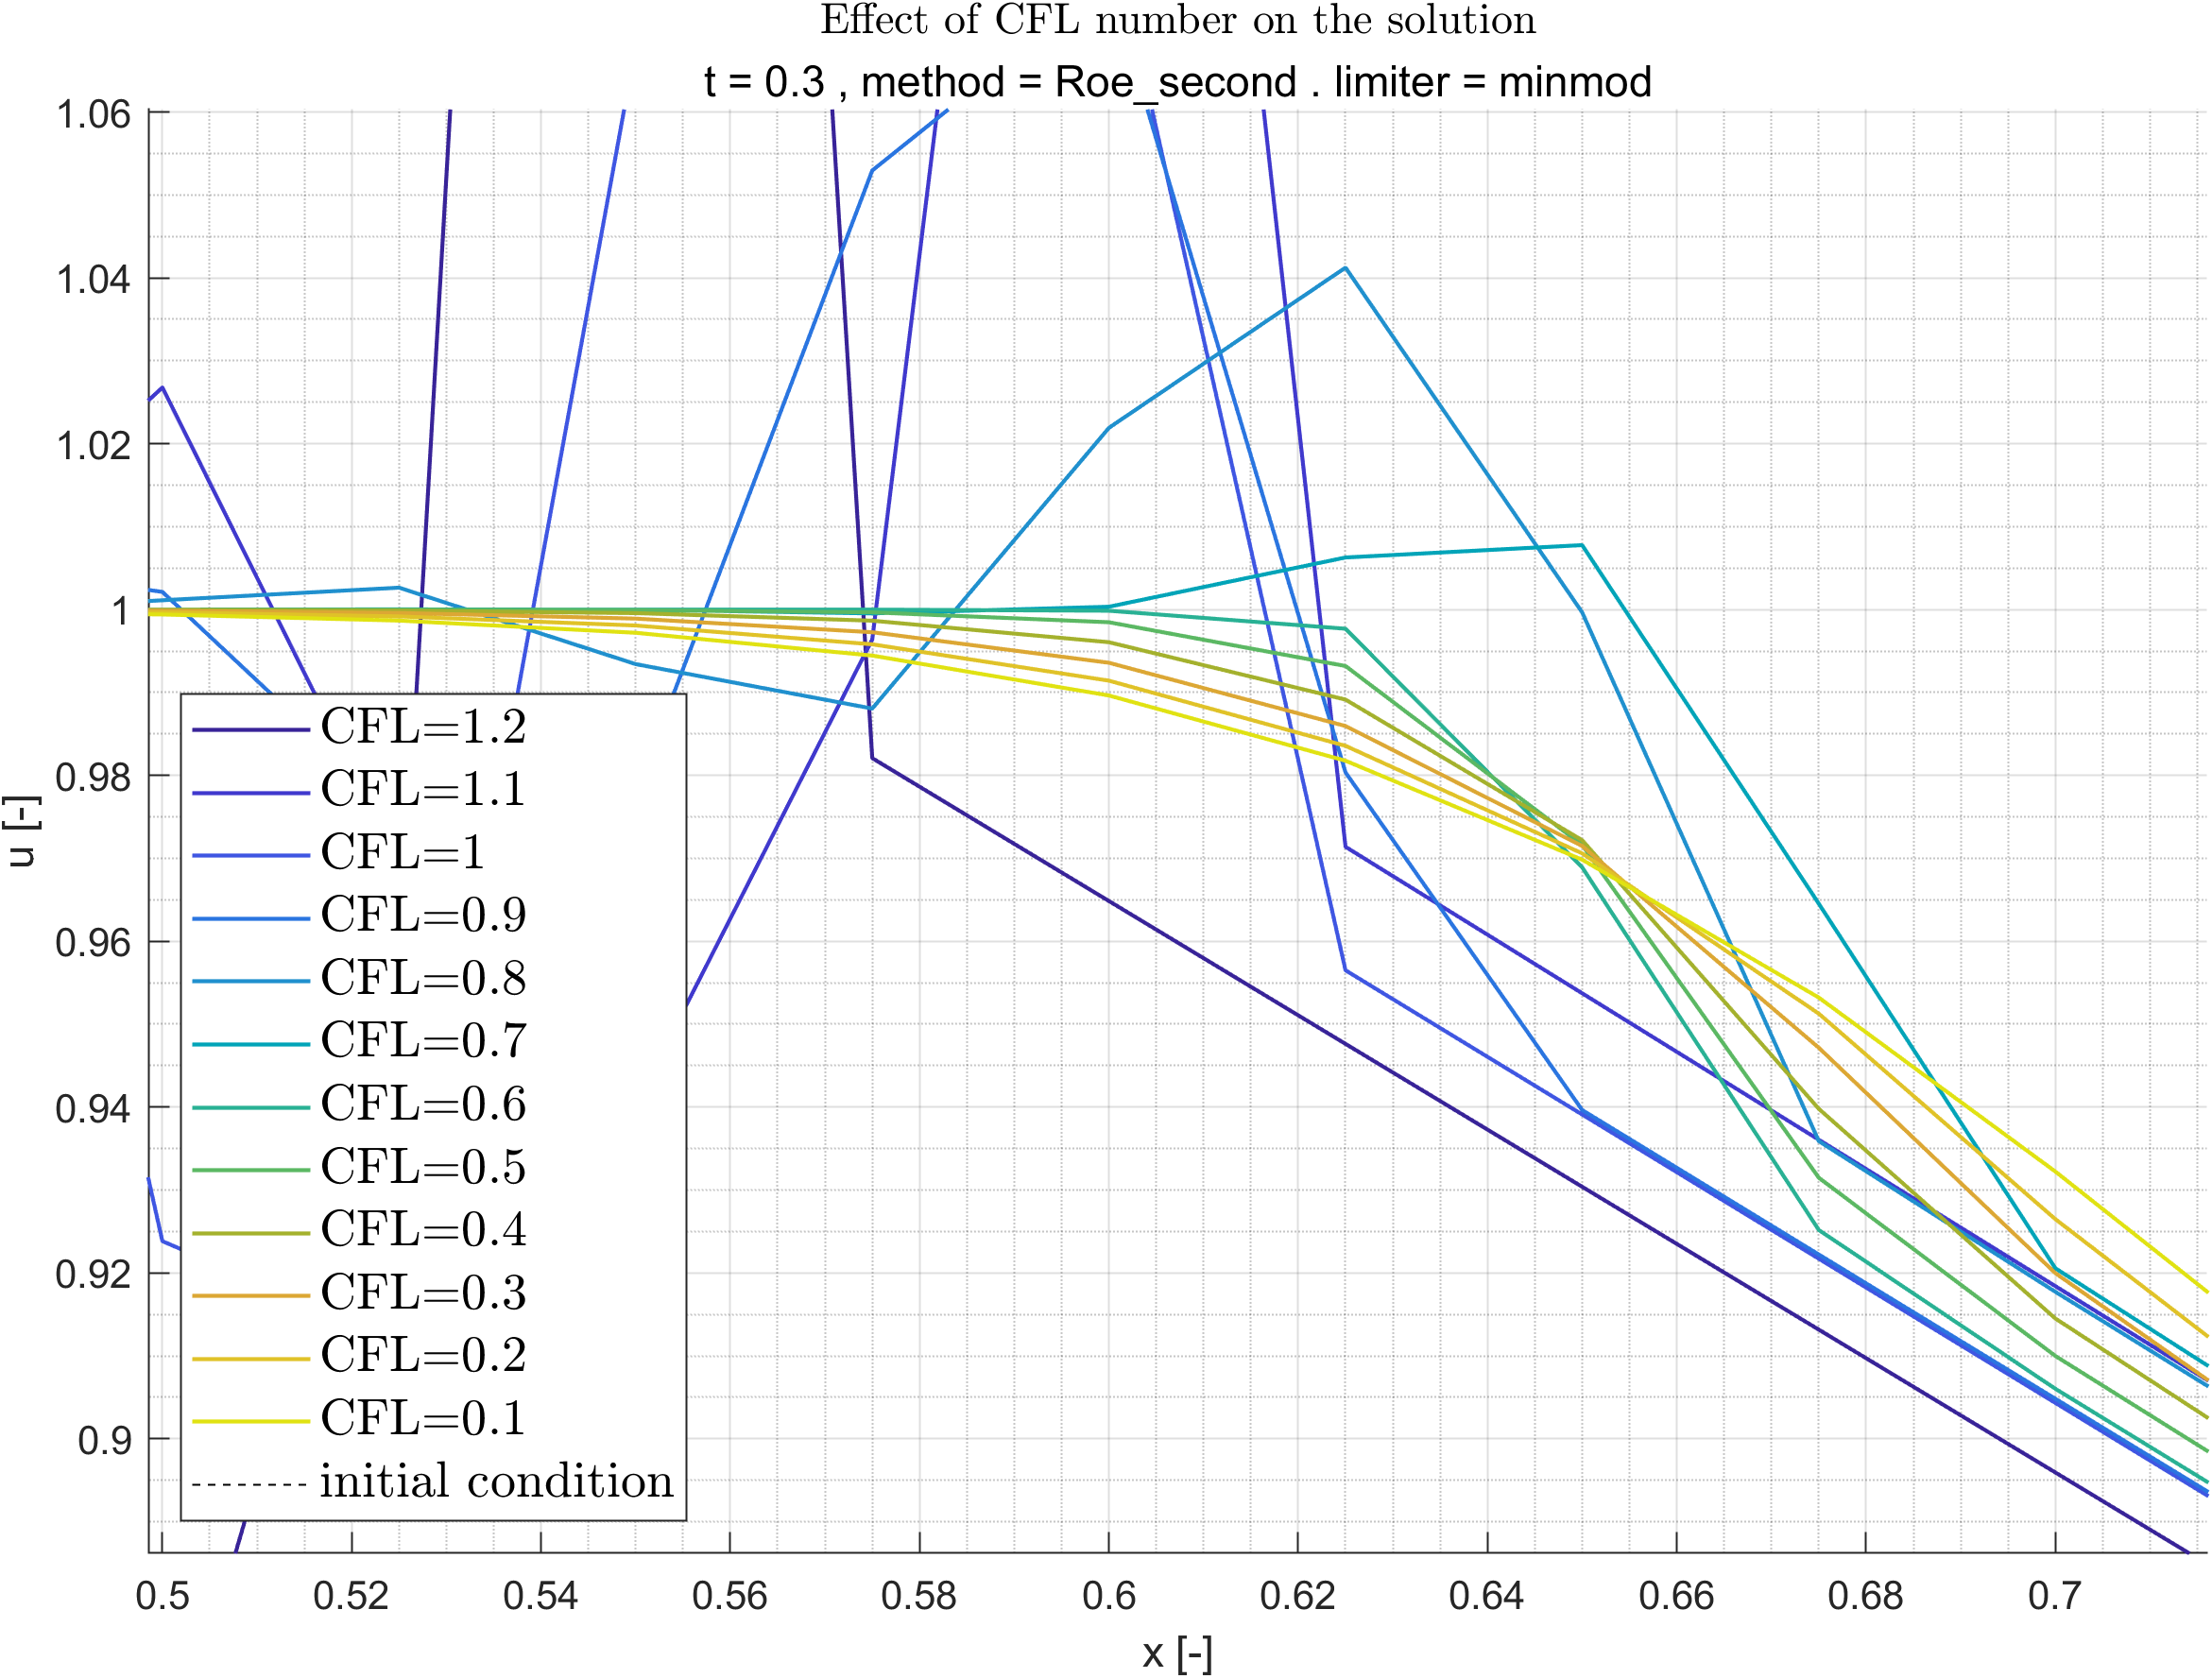
\includegraphics[width=\textwidth]{images/grap6.1.png}
        \caption{minmod - zoomed}
        \label{fig:roe_second_minmod_B}
    \end{subfigure}
    \caption{Effect of CFL number on solution - Roe second order with different limiters}
    \label{fig:roe_second_with_limiters}
\end{figure}
\noindent We can see that when there are limiters, for a CFL number bigger than 0.8, there are oscillations far from the wavefront, but unlike the case with no limiters, the solution does converge. At low CFL numbers, the oscillations are not pronounced since the time step is really small, except for the van Leer limiter, at which the oscillations are never negligible. The oscillations starts the closest to the wavefront when using the van Leer limiter. 

\subsubsection{Effect of Limiter}
\begin{figure}[H]
    \centering
    \begin{subfigure}[c]{.49\textwidth}
        \centering
        \includegraphics[width=\textwidth]{images/grap7.png}
        \caption{difference limiters}
        \label{fig:roe_second_diff_limiters_A}
    \end{subfigure}
    \hfill
    \begin{subfigure}[c]{.49\textwidth}
        \centering
        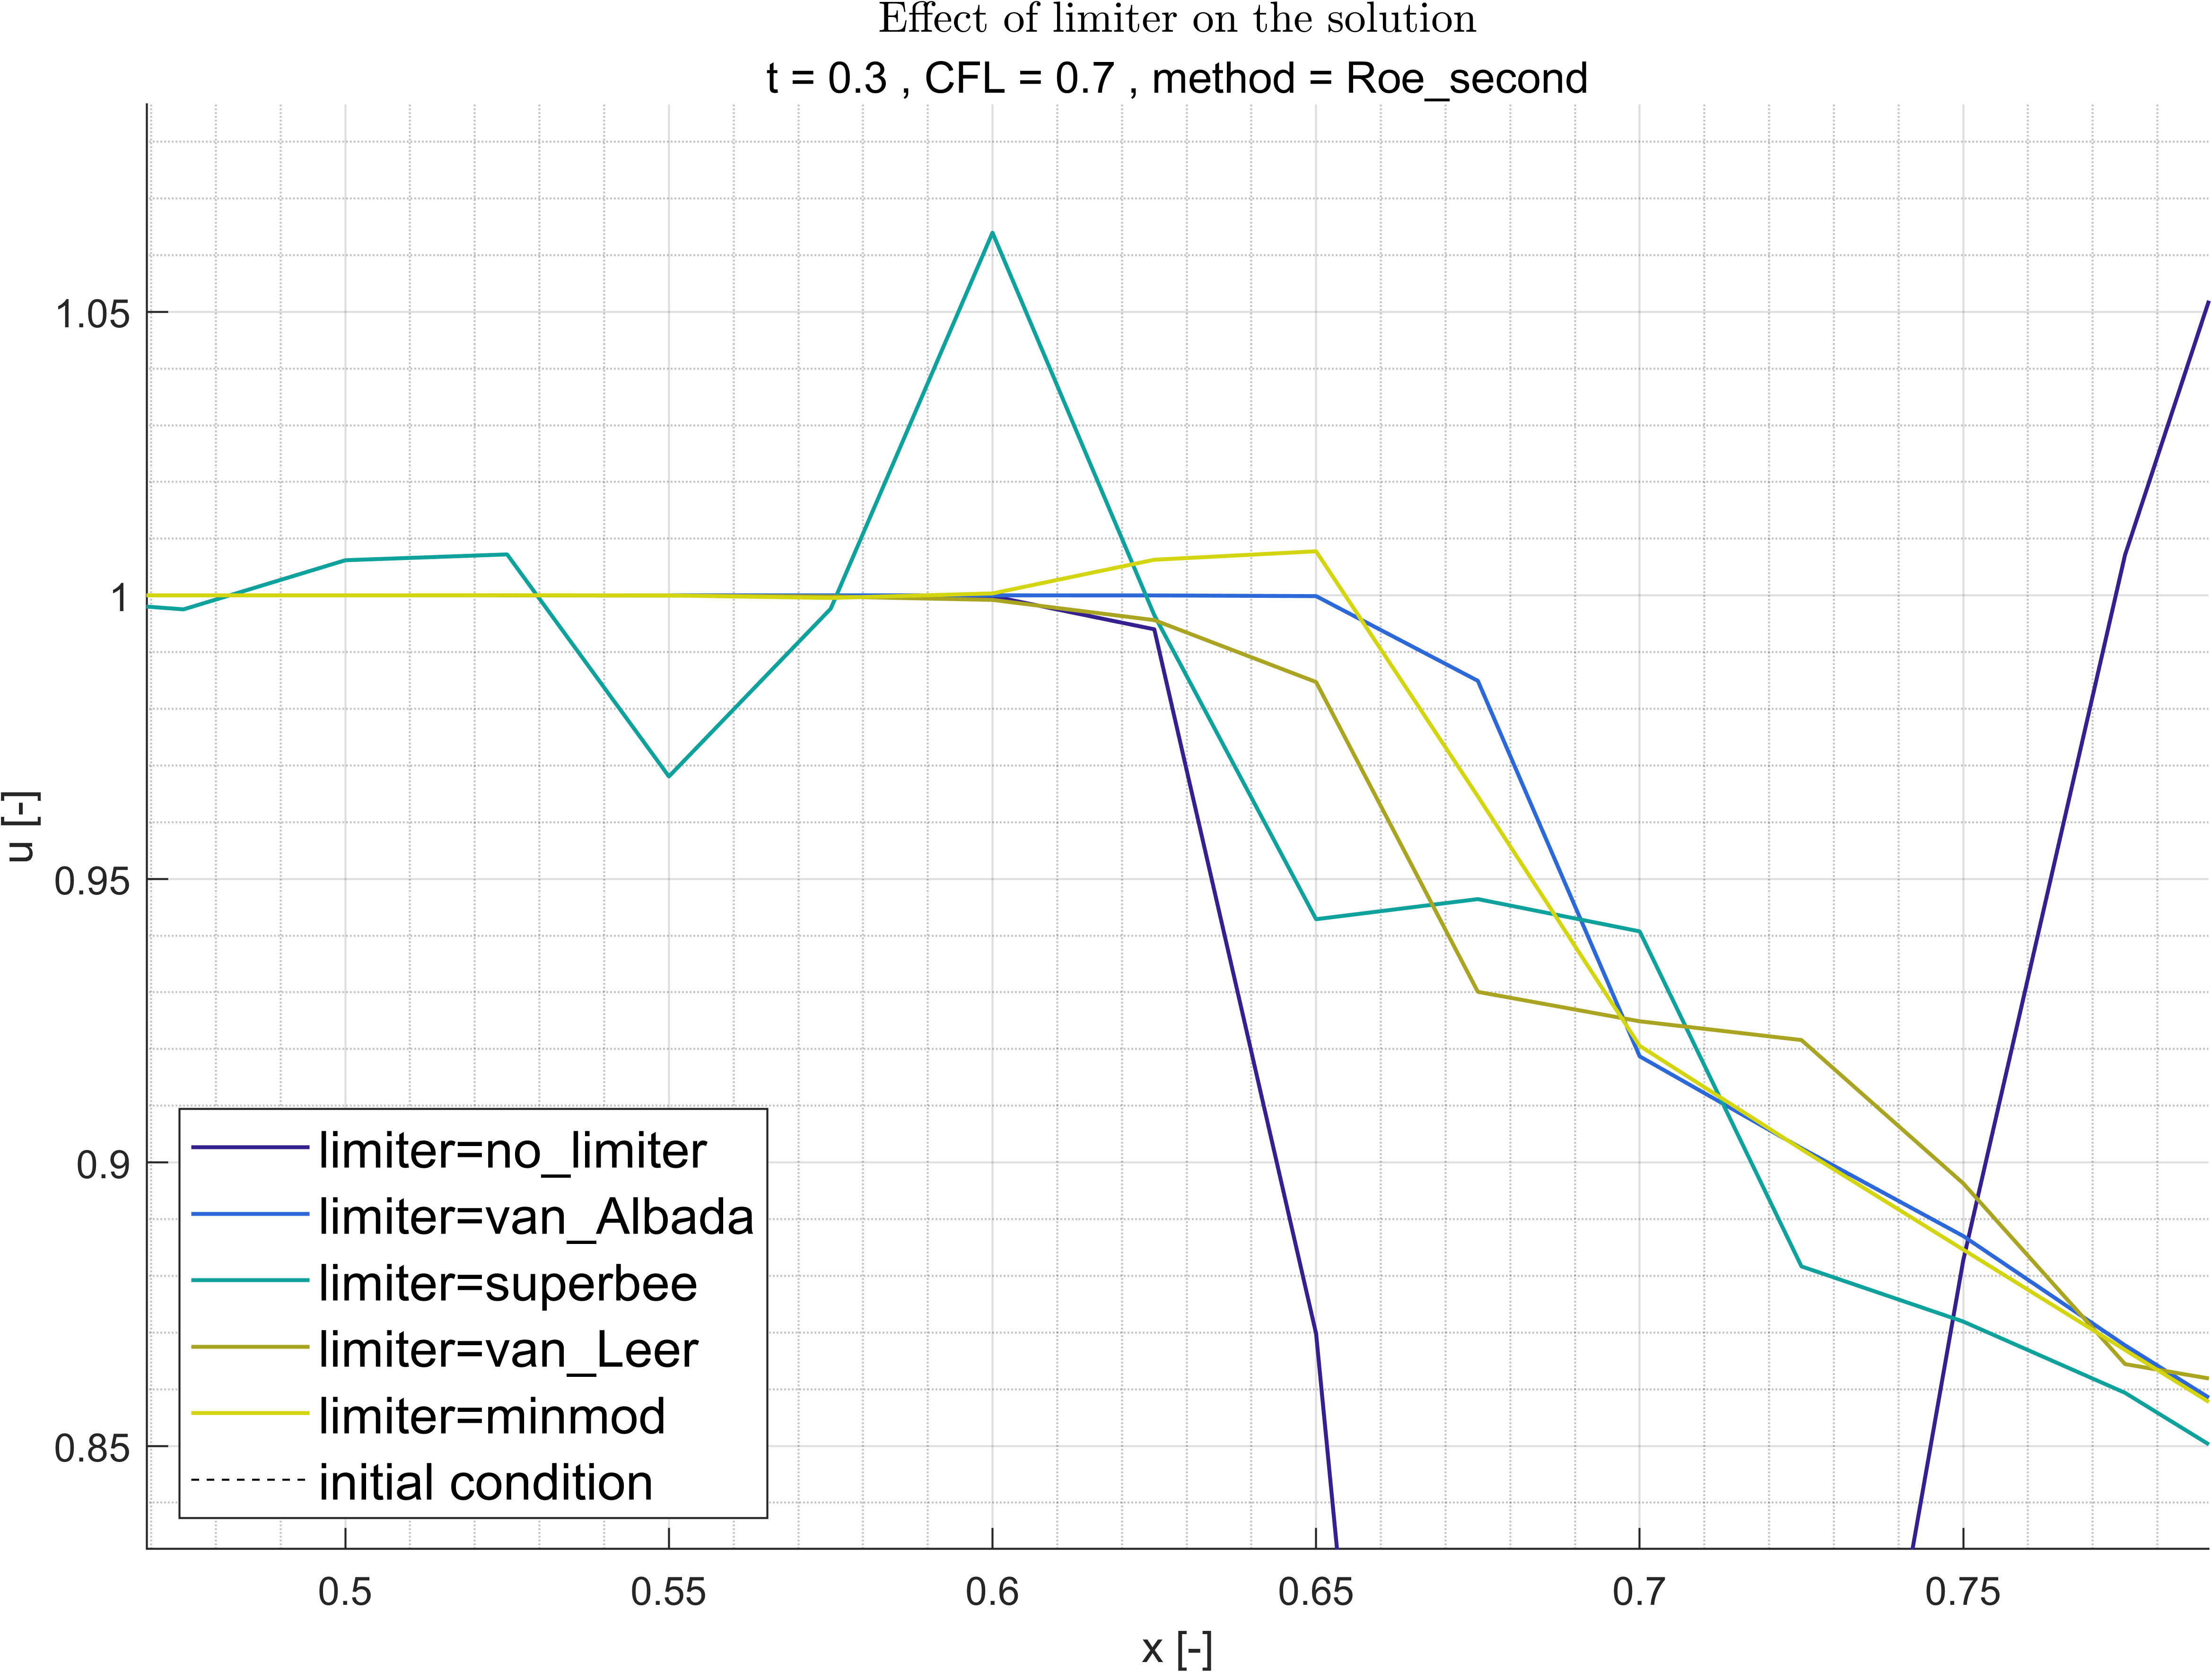
\includegraphics[width=\textwidth]{images/grap7.1.png}
        \caption{difference limiters - zoomed}
        \label{fig:roe_second_diff_limiters_B}
    \end{subfigure}
    \caption{Effect of limiters on solution}
    \label{fig:roe_second_difference_limiters}
\end{figure}
We can that the addition of a limiter dampens the oscillations and makes the scheme converge for larger CFL numbers. With Figure \ref{fig:roe_second_difference_limiters} it is clear that most limiters keep the wavefront linear except for the van Leer limiter, which only dampens the oscillations at the wavefront.
\newpage

\section{Generalized Burgers Equation}
The generalized Burgers equation is given by:
\begin{equation}
    \frac{\partial u}{\partial t}+\left(c+bu\right)\frac{\partial u}{\partial x}=\mu\frac{\partial^2u}{\partial x^2}
\end{equation}
Where:
\begin{equation*}
    \begin{matrix}
        c=\frac{1}{2} && b=-1 && \mu=\left[0.001, 0.25\right]
    \end{matrix}
\end{equation*}
The equation can also be presented as:
\begin{equation}
    \begin{matrix}
        \displaystyle\frac{\partial u}{\partial t}+\frac{\partial\bar{F}}{\partial x}=0 && \bar{F}=\underbrace{cu+\frac{bu^2}{2}}_F-\underbrace{\mu\frac{\partial u}{\partial x}}_{F_\nu}
    \end{matrix}
\end{equation}
In non-conservation law form, is given by:
\begin{equation}
    \begin{matrix}
        \displaystyle\frac{\partial u}{\partial t}+A\frac{\partial u}{\partial x}=0 && \displaystyle A=\frac{\partial\bar{F}}{\partial u}=c+bu-\mu\frac{\partial}{\partial u}\left(\frac{\partial u}{\partial x}\right)
    \end{matrix}
\end{equation}
The generalized Burgers equation has a stationary solution:
\begin{equation}
    u=-\frac{c}{b}\left(1+\tanh{\left(\displaystyle\frac{c\left(x-x_0\right)}{2\mu}\right)}\right)
\end{equation}

\subsection{Domain and Computational Mesh}
Using 41 grid points with $\Delta x=1$ and computing until $t=18.0$. $\Delta t=\left[0.5, 1.0\right]$.

\subsection{Boundary and Initial Conditions}
\subsubsection{Initial Conditions}
\begin{equation}
    u_{\left(x,t=0\right)}=\frac{1}{2}\left(1+\tanh\left(250\left(x-20\right)\right)\right)
\end{equation}
\subsubsection{Boundary Conditions}
Using Dirichlet boundary conditions:
\begin{equation}
    \begin{matrix}
        \displaystyle u_{\left(x=0,t\right)}=0 && \displaystyle u_{\left(x=40,t\right)}=1
    \end{matrix}
\end{equation}

\subsection{First Order Roe Method (explicit)}
As written above for the inviscid Burgers equation (\ref{Roe_first}), Roes scheme is based on the solution of the linear problem:
\begin{equation}
    \begin{matrix}
        \displaystyle\frac{\partial u}{\partial t} + \bar{A}\frac{\partial u}{\partial x}=\mu\frac{\partial^2u}{\partial x^2} && \displaystyle \bar{A}=\frac{\partial F}{\partial u}
    \end{matrix}         
\end{equation}
In the case of the Burgers equation, the matrix $\bar{A}$ is a scalar.
\begin{equation}
    \bar{A}=\bar{A}_{i+\frac{1}{2}}=\frac{F_{i+1}-F_i}{u_{i+1}-u_i}=\left\{\begin{array}{cc} \displaystyle\frac{\displaystyle c\left(u_{i+1}-u_i\right)+\frac{b}{2}\left(u_{i+1}^2-u_i^2\right)}{u_{i+1}-u_i} & u_i\neq u_{i+1} \\ 
    A_i & u_i=u_{i+1} \end{array}\right.  
\end{equation} 
The numerical flux at the cell interface:
\begin{equation}
    \displaystyle \bar{f}_{i+\frac{1}{2}}=\frac{F_i+F_{i+1}}{2}-\frac{1}{2}\left(\bar{A}_{i+\frac{1}{2}}^+-\bar{A}_{i+\frac{1}{2}}^-\right)\left(u_{i+1}-u_i\right)
\end{equation}
Where:
\begin{equation}
    \left\{\begin{array}{cc}
        \begin{array}{c}
            \bar{A}_{i+\frac{1}{2}}^+\triangleq\displaystyle\frac{1}{2}\left(\bar{A}{i+\frac{1}{2}}+\left|\bar{A}_{i+\frac{1}{2}}\right|\right)\geq0 \\\\
            \bar{A}_{i+\frac{1}{2}}^-\triangleq\displaystyle\frac{1}{2}\left(\bar{A}_{i+\frac{1}{2}}-\left|\bar{A}_{i+\frac{1}{2}}\right|\right)\leq0 \\
        \end{array} & \bar{A}_{i+\frac{1}{2}}=\bar{A}_{i+\frac{1}{2}}^++\bar{A}_{i+\frac{1}{2}}^-
    \end{array}\right.
\end{equation}

% In the case of the Burgers equation, the matrix $\bar{A}$ is a scalar, namely, $\bar{A}=\bar{u}$. The equation becomes: \begin{equation} \displaystyle\frac{\partial u}{\partial t} + \bar{u}\frac{\partial u}{\partial x}=\mu\frac{\partial^2u}{\partial x^2} \end{equation} \begin{equation} \bar{u}=\bar{u}_{i+\frac{1}{2}}=\frac{F_{i+1}-F_i}{u_{i+1}-u_i}=\left\{\begin{array}{cc} \displaystyle\frac{\displaystyle c\left(u_{i+1}-u_i\right)+\frac{b}{2}\left(u_{i+1}^2-u_i^2\right)}{u_{i+1}-u_i} & u_i\neq u_{i+1} \\ u_i & u_i=u_{i+1} \end{array}\right.  \end{equation} The numerical flux at the cell interface:
% \begin{equation}
%     \displaystyle \bar{f}_{i+\frac{1}{2}}=\frac{F_i+F_{i+1}}{2}-\frac{1}{2}\left(\bar{u}_{i+\frac{1}{2}}^+-\bar{u}_{i+\frac{1}{2}}^-\right)\left(u_{i+1}-u_i\right)
% \end{equation}
% Where:
% \begin{equation}
%     \left\{\begin{array}{cc}
%         \begin{array}{c}
%             \bar{u}_{i+\frac{1}{2}}^+\triangleq\displaystyle\frac{1}{2}\left(\bar{u}{i+\frac{1}{2}}+\left|\bar{u}_{i+\frac{1}{2}}\right|\right)\geq0 \\\\
%             \bar{u}_{i+\frac{1}{2}}^-\triangleq\displaystyle\frac{1}{2}\left(\bar{u}_{i+\frac{1}{2}}-\left|\bar{u}_{i+\frac{1}{2}}\right|\right)\leq0 \\
%         \end{array} & \bar{u}_{i+\frac{1}{2}}=\bar{u}_{i+\frac{1}{2}}^++\bar{u}_{i+\frac{1}{2}}^-
%     \end{array}\right.
% \end{equation}
And finally:
\begin{equation}
    u_i^{n+1}=u_i^n-\frac{\Delta t}{\Delta x}\left(\bar{f}_{i+\frac{1}{2}}^n-\bar{f}_{i-\frac{1}{2}}^n\right)+\mu\frac{\Delta t}{\left(\Delta x\right)^2}\left(u_{i+1}^n-2u_i^n+u_{i-1}^n\right)
\end{equation}

% MY WAY

% As written above for the inviscid Burgers equation (\ref{Roe_first}), Roes scheme is based on the solution of the linear problem:
% \begin{equation}
%         \displaystyle\frac{\partial u}{\partial t} + \bar{A}\frac{\partial u}{\partial x} = 0 
% \end{equation}
% Where $\bar{A}$ is a constant matrix that is dependent on local conditions. The matrix is constructed in a way that guarantees uniform validity across discontinuities: 
% \begin{enumerate}
%     \item For any $u_i$, $u_{i+1}$:\begin{equation*}
%         \bar{F}{i+1}-\bar{F}{i} = \bar{A}\cdot\left(u_{i+1}-u_i\right)
%     \end{equation*}
%     \item When $u=u_i=u_{i+1}$ then:\begin{equation*}
%         \bar{A}{\left(u_i,u{i+1}\right)}=\bar{A}_{\left(u,u\right)}=\frac{\partial \bar{F}}{\partial u}
%     \end{equation*}
% \end{enumerate}
% In the case of the Burgers equation, the matrix $\bar{A}$ is a scalar. The value of $\bar{A}$ for the cell face between \emph{i} and \emph{i+1} is determined from the first conditions, using central difference for the viscus term (forward/backward at the edges):
% \begin{equation}
%     \begin{array}{c}
%         \bar{A}=\bar{A}{i+\frac{1}{2}}=\displaystyle\frac{\bar{F}{i+1}-\bar{F}i}{u{i+1}-u_i}=\frac{\displaystyle c\left(u_{i+1}-u_i\right)+\frac{b}{2}\left(u_{i+1}^2-u_{i}^2\right)-\mu\left(\left.\frac{\partial u}{\partial x}\right|{i+1}-\left.\frac{\partial u}{\partial x}\right|{i}\right)}{u_{i+1}-u_i}
%         % \\ \Downarrow \\
%         % A=\frac{\displaystyle c\left(u_{i+1}-u_i\right)+\frac{b}{2}\left(u_{i+1}^2-u_{i}^2\right)-\mu\left(\left.\frac{\partial u}{\partial x}\right|{i+1}-\left.\frac{\partial u}{\partial x}\right|{i}\right)}{u_{i+1}-u_i}
%     \end{array}   
% \end{equation}
% The numerical flux at the cell interface:
% \begin{equation}
%     \displaystyle \bar{f}{i+\frac{1}{2}}=\frac{\bar{F}_i+\bar{F}{i+1}}{2}-\frac{1}{2}\left(\bar{A}{i+\frac{1}{2}}^+-\bar{A}{i+\frac{1}{2}}^-\right)\left(u_{i+1}-u_i\right)
% \end{equation}
% Where:
% \begin{equation}
%     \left\{\begin{array}{cc}
%         \begin{array}{c}
%             \bar{A}{i+\frac{1}{2}}^+\triangleq\displaystyle\frac{1}{2}\left(\bar{A}{i+\frac{1}{2}}+\left|\bar{A}_{i+\frac{1}{2}}\right|\right)\geq0 \\\\
%             \bar{A}{i+\frac{1}{2}}^-\triangleq\displaystyle\frac{1}{2}\left(\bar{A}{i+\frac{1}{2}}-\left|\bar{A}_{i+\frac{1}{2}}\right|\right)\leq0 \\
%         \end{array} & \bar{A}{i+\frac{1}{2}}=\bar{A}{i+\frac{1}{2}}^++\bar{A}_{i+\frac{1}{2}}^-
%     \end{array}\right.
% \end{equation}
% And finally:
% \begin{equation}
%     u_i^{n+1}=u_i^n-\frac{\Delta t}{\Delta x}\left(\bar{f}{i+\frac{1}{2}}^n-\bar{f}{i-\frac{1}{2}}^n\right)
% \end{equation}

\subsubsection{Effect of Time Step}
\begin{figure}[H]
    \centering
    \begin{subfigure}[c]{.49\textwidth}
        \centering
        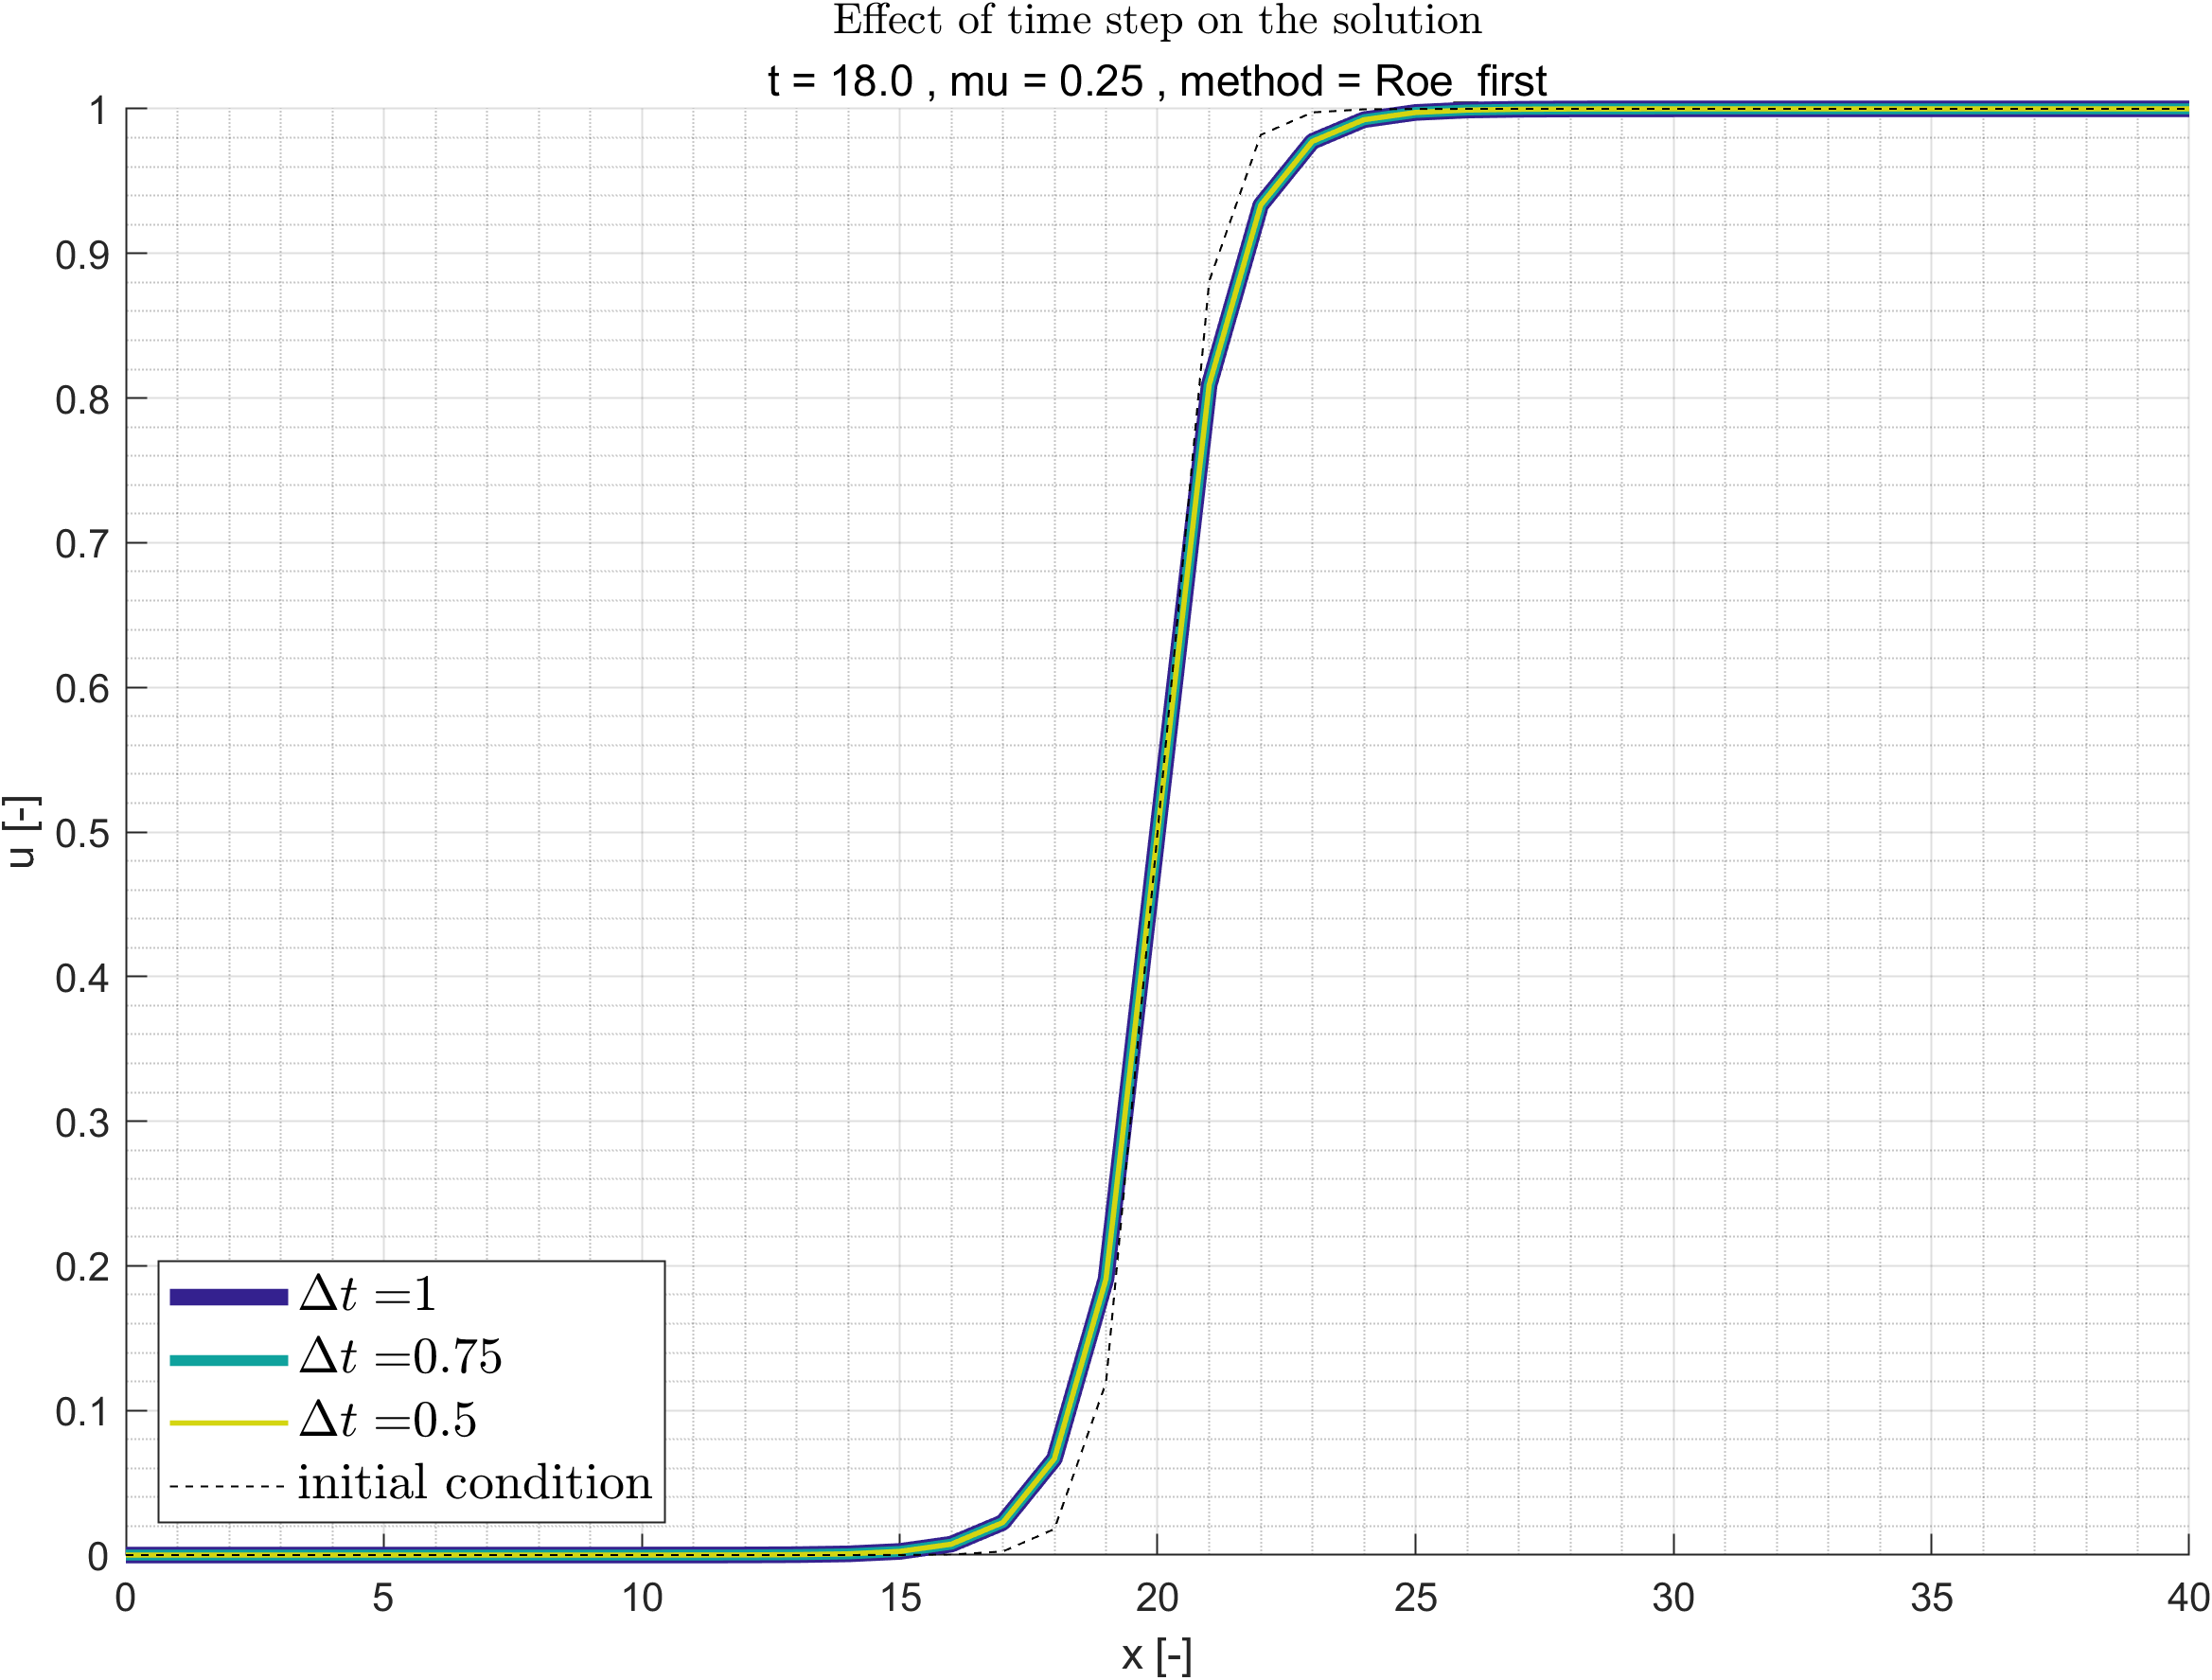
\includegraphics[width=\textwidth]{images/grap8.png}
        \caption{roe first $\mu=0.25$ difference limiters}
        \label{fig:roe_first_general_mu0.25_A}
    \end{subfigure}
    \hfill
    \begin{subfigure}[c]{.49\textwidth}
        \centering
        \includegraphics[width=\textwidth]{images/grap8.1.png}
        \caption{roe first $\mu=0.25$ difference limiters - zoomed}
        \label{fig:roe_first_general_mu0.25_B}
    \end{subfigure}
    \begin{subfigure}[c]{.49\textwidth}
        \centering
        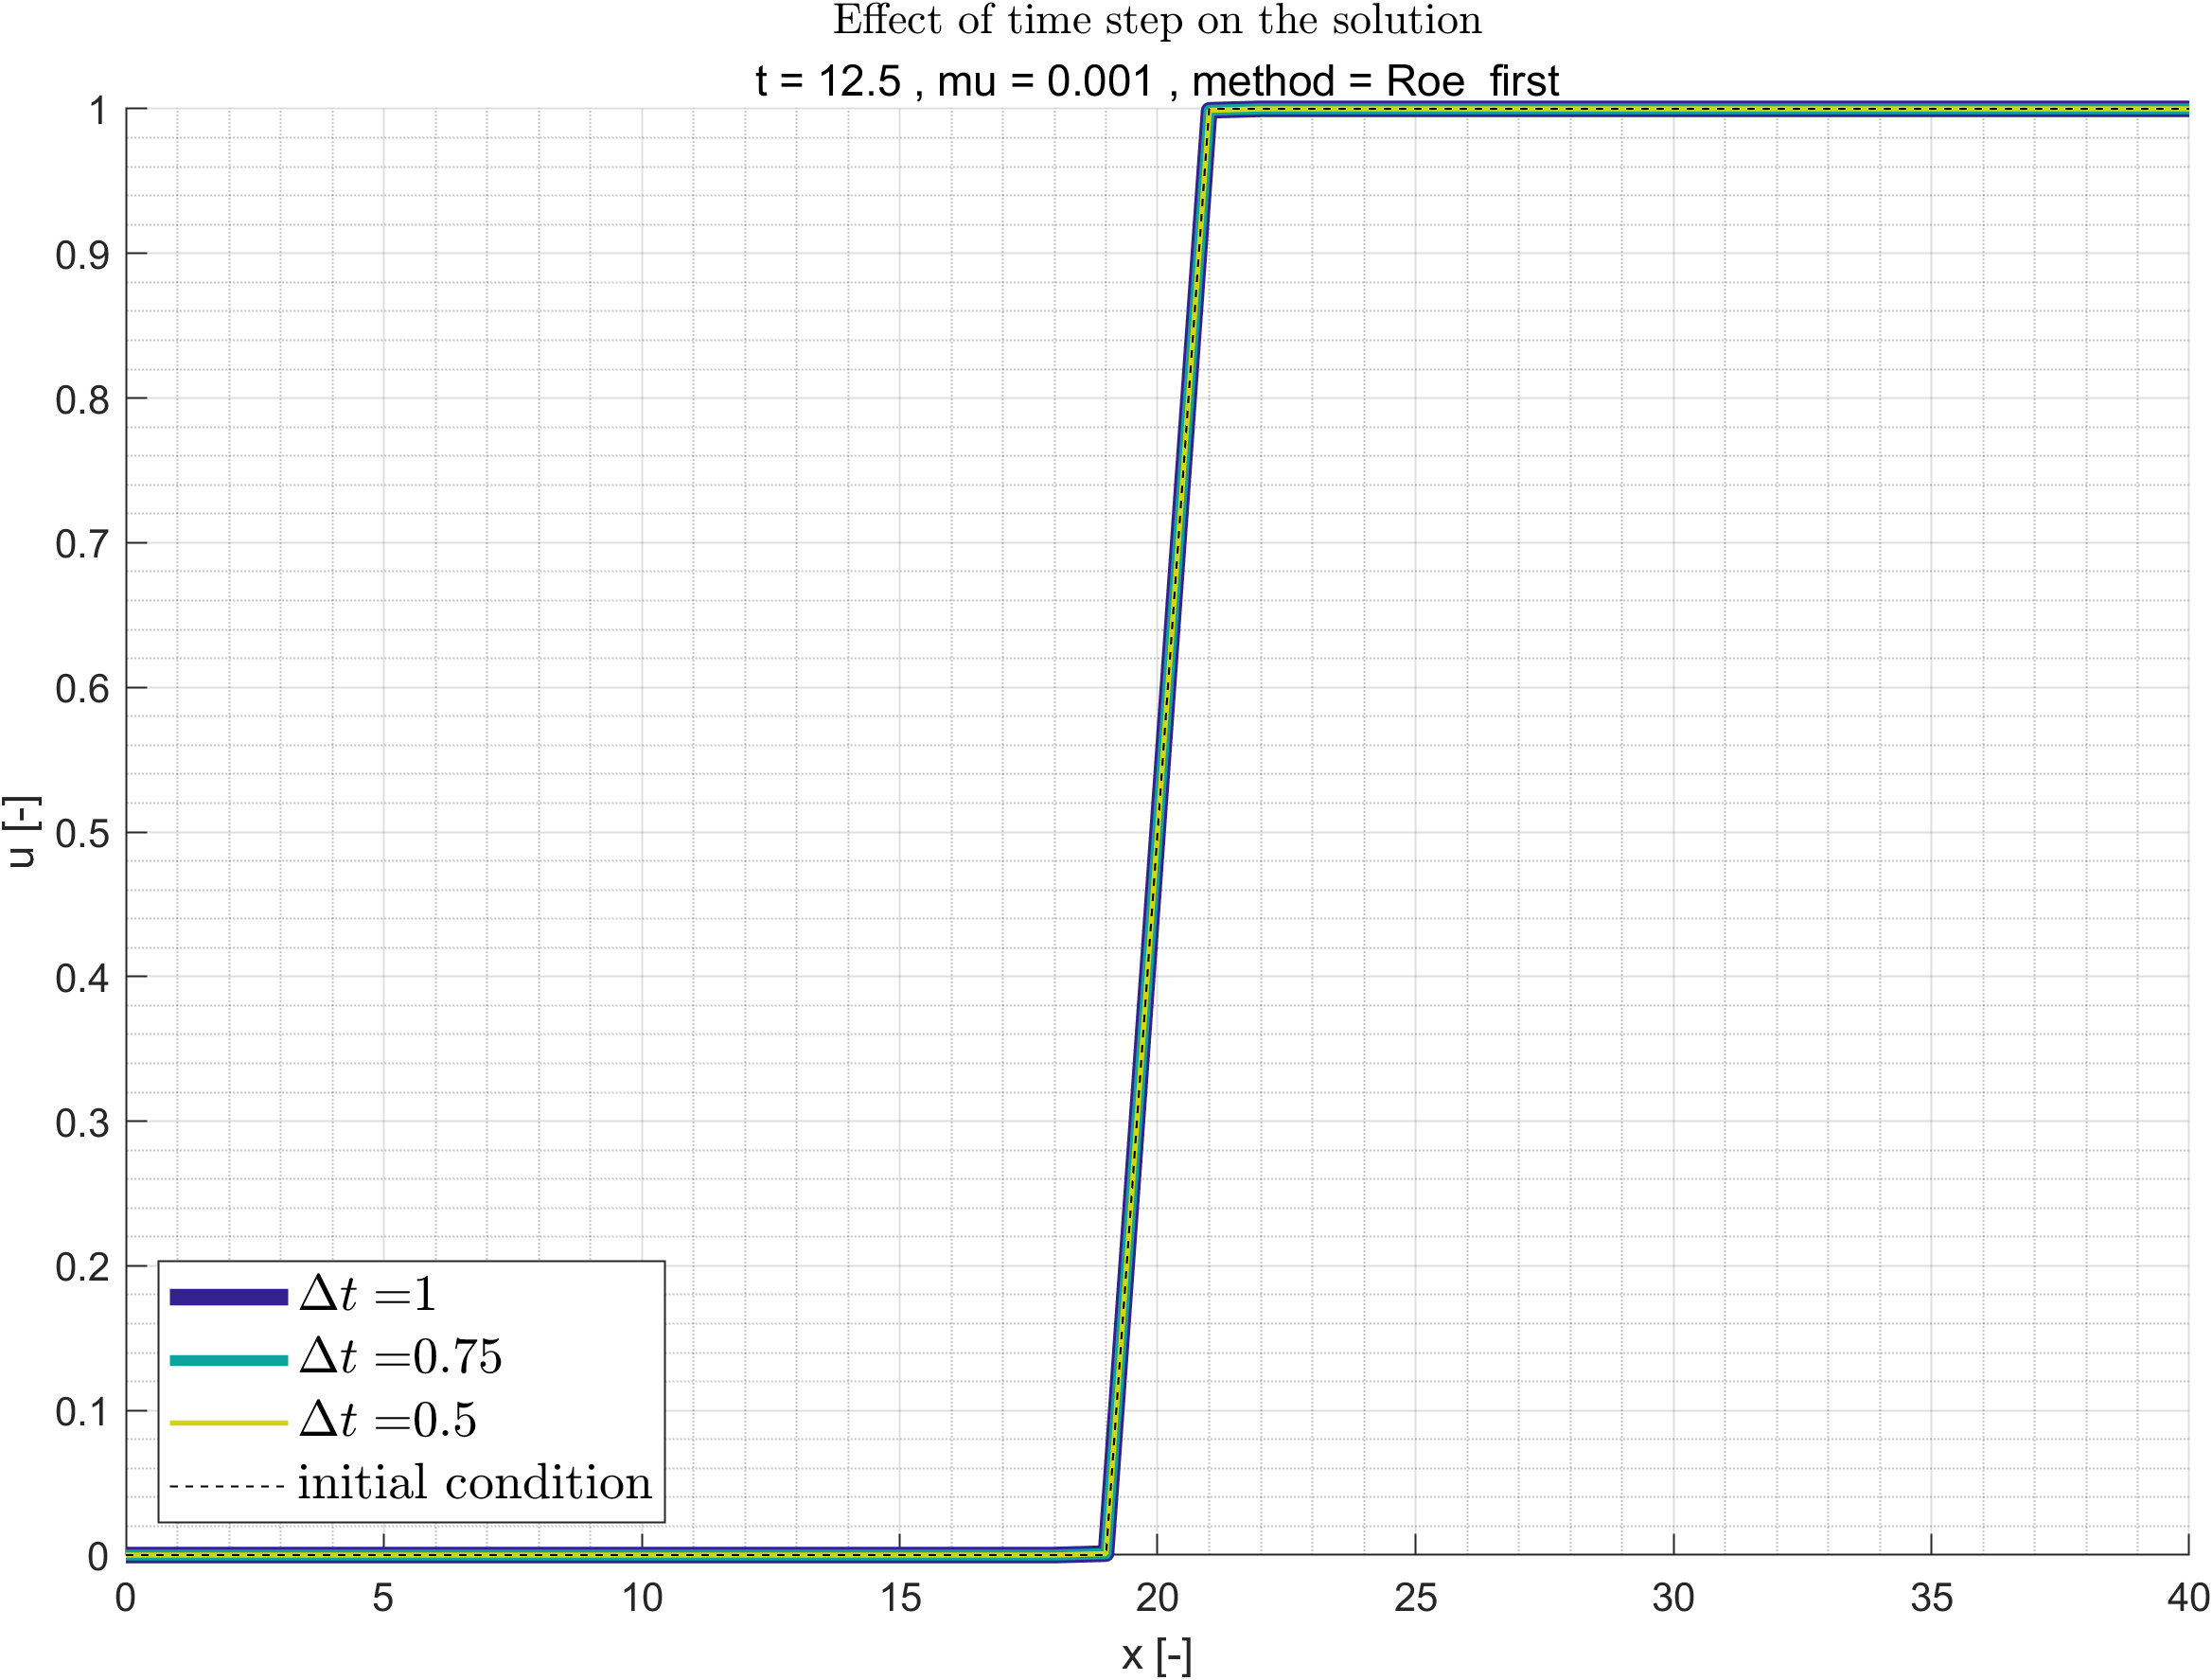
\includegraphics[width=\textwidth]{images/grap9.png}
        \caption{roe first $\mu=0.001$ difference limiters}
        \label{fig:roe_first_general_mu0.001_A}
    \end{subfigure}
    \hfill
    \begin{subfigure}[c]{.49\textwidth}
        \centering
        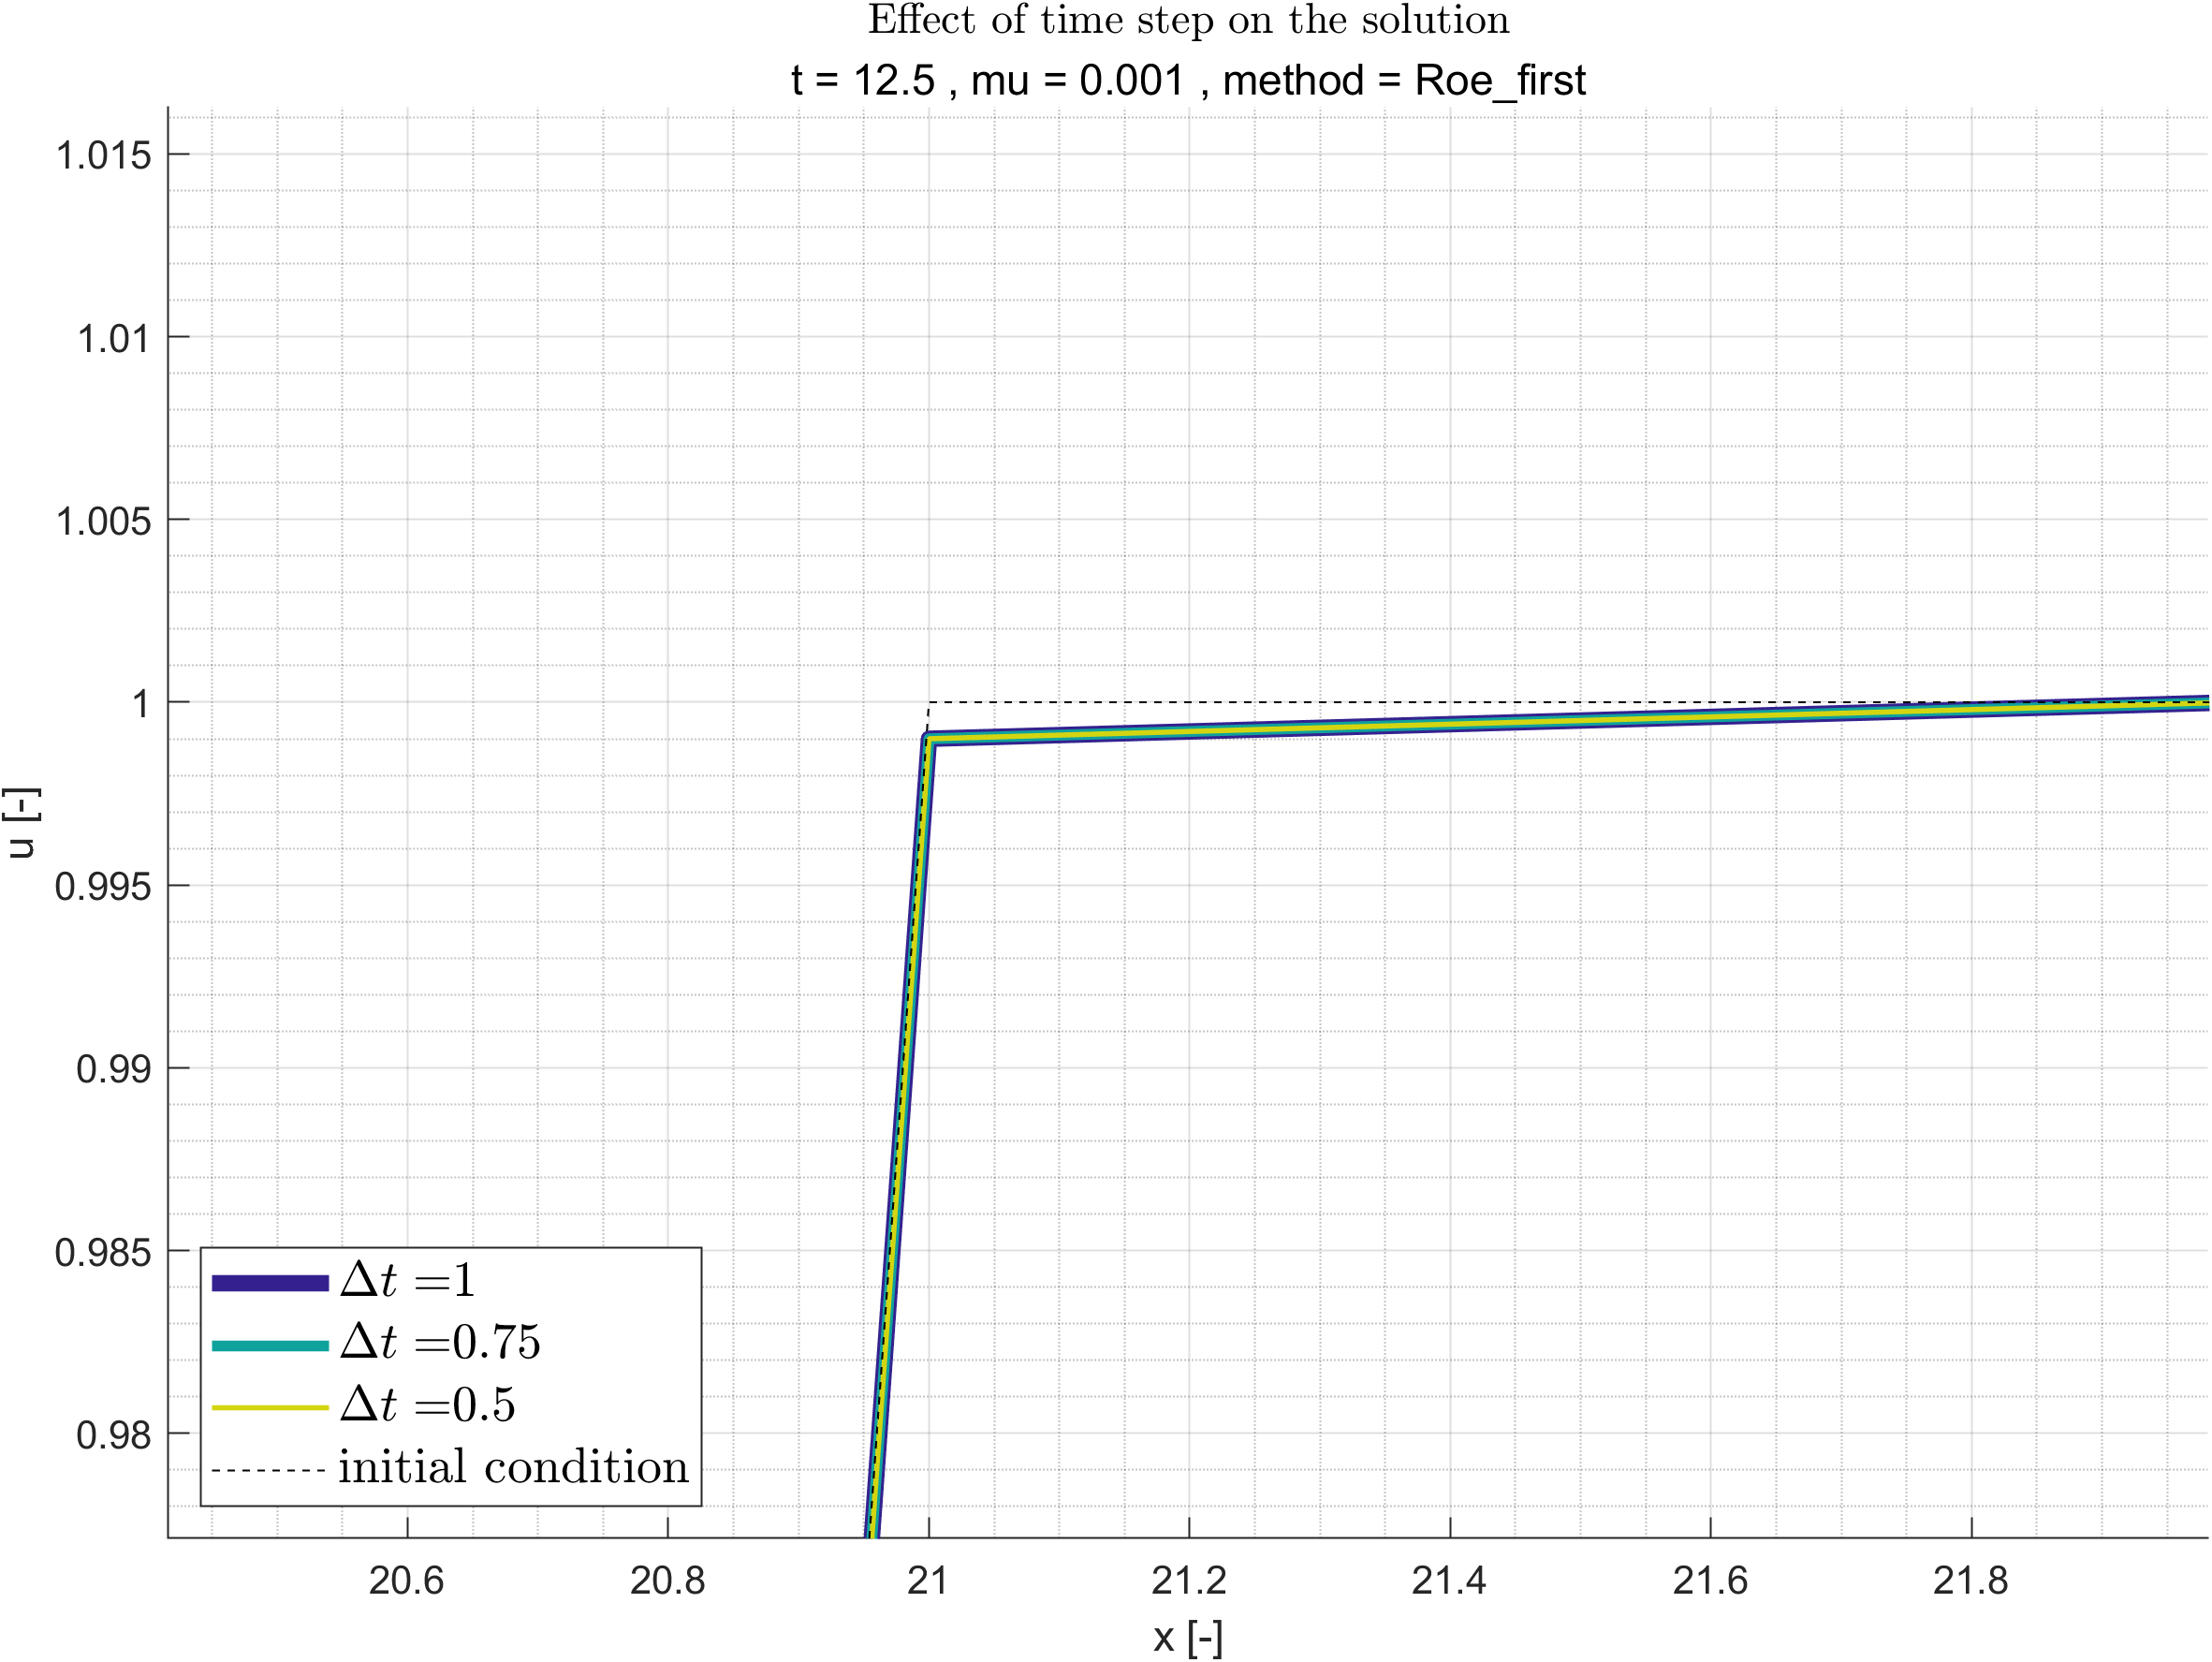
\includegraphics[width=\textwidth]{images/grap9.1.png}
        \caption{roe first $\mu=0.001$ difference limiters - zoomed}
        \label{fig:roe_first_general_mu0.001_B}
    \end{subfigure}
    \caption{Effect of time step on solution - Roe first order - generalized}
        \label{fig:roe_first_general}
\end{figure}
We can see that in the case of Roe's first order, there is no effect of the time step on the solution with no connection to the viscosity $\left(\mu\right)$. The wave is indeed diffused like expected since this is a first-order method and they are diffusives. 

\subsection{MacCormack Method}
The original MacCormack method applied to Burgers equaiton results in:
\begin{equation}
    \begin{array}{cc}
        \displaystyle\mathrm{Predictor:} & \displaystyle u_i^{\overline{n+1}}=u_i^n-\Delta t\frac{\Delta F_i^n}{\Delta x}+r\delta^2u_i^n \\\\ 
        \displaystyle\mathrm{Corrector:} & \displaystyle u_i^{n+1}=\frac{1}{2}\left(u_i^n+u_i^{\overline{n+1}}-\Delta t\frac{\nabla F_i^{\overline{n+1}}}{\Delta x}\right)+r\delta^2u_i^{\overline{n+1}}
    \end{array}
\end{equation}
Where:
\begin{itemize}
    \item $\displaystyle r=\frac{\mu\Delta t}{\left(\Delta x\right)^2}$
    \item $\displaystyle \delta^2u_i=u_{i+1}-2u_i+u_{i-1}$
    \item $\Delta f=f_{i+1}-f_i$
    \item $\nabla f=f_i-f_{i-1}$
\end{itemize}
% \begin{equation*}
%     \Downarrow
% \end{equation*}
% \begin{equation}
%     \begin{array}{cc}
%         \displaystyle\mathrm{Predictor:} & \displaystyle u_i^{\overline{n+1}}=u_i^n-\Delta t\frac{F_{i+1}^n-F_{i}^n}{\Delta x}+r\delta^2u_i^n \\\\ 
%         \displaystyle\mathrm{Corrector:} & \displaystyle u_i^{n+1}=\frac{1}{2}\left(u_i^n+u_i^{\overline{n+1}}-\Delta t\frac{\nabla F_i^{\overline{n+1}}}{\Delta x}\right)+r\delta^2u_i^{\overline{n+1}}
%     \end{array}
% \end{equation}

% \subsubsection{Stability}
% The stability condition for MacCormack's method is:
% \begin{equation}
%     \Delta t\le\frac{\left(\Delta x\right)^2}{\left|u\right|\Delta x+\mu}
% \end{equation}
\subsubsection{Effect of Time Step}
\begin{figure}[H]
    \centering
    \begin{subfigure}[c]{.39\textwidth}
        \centering
        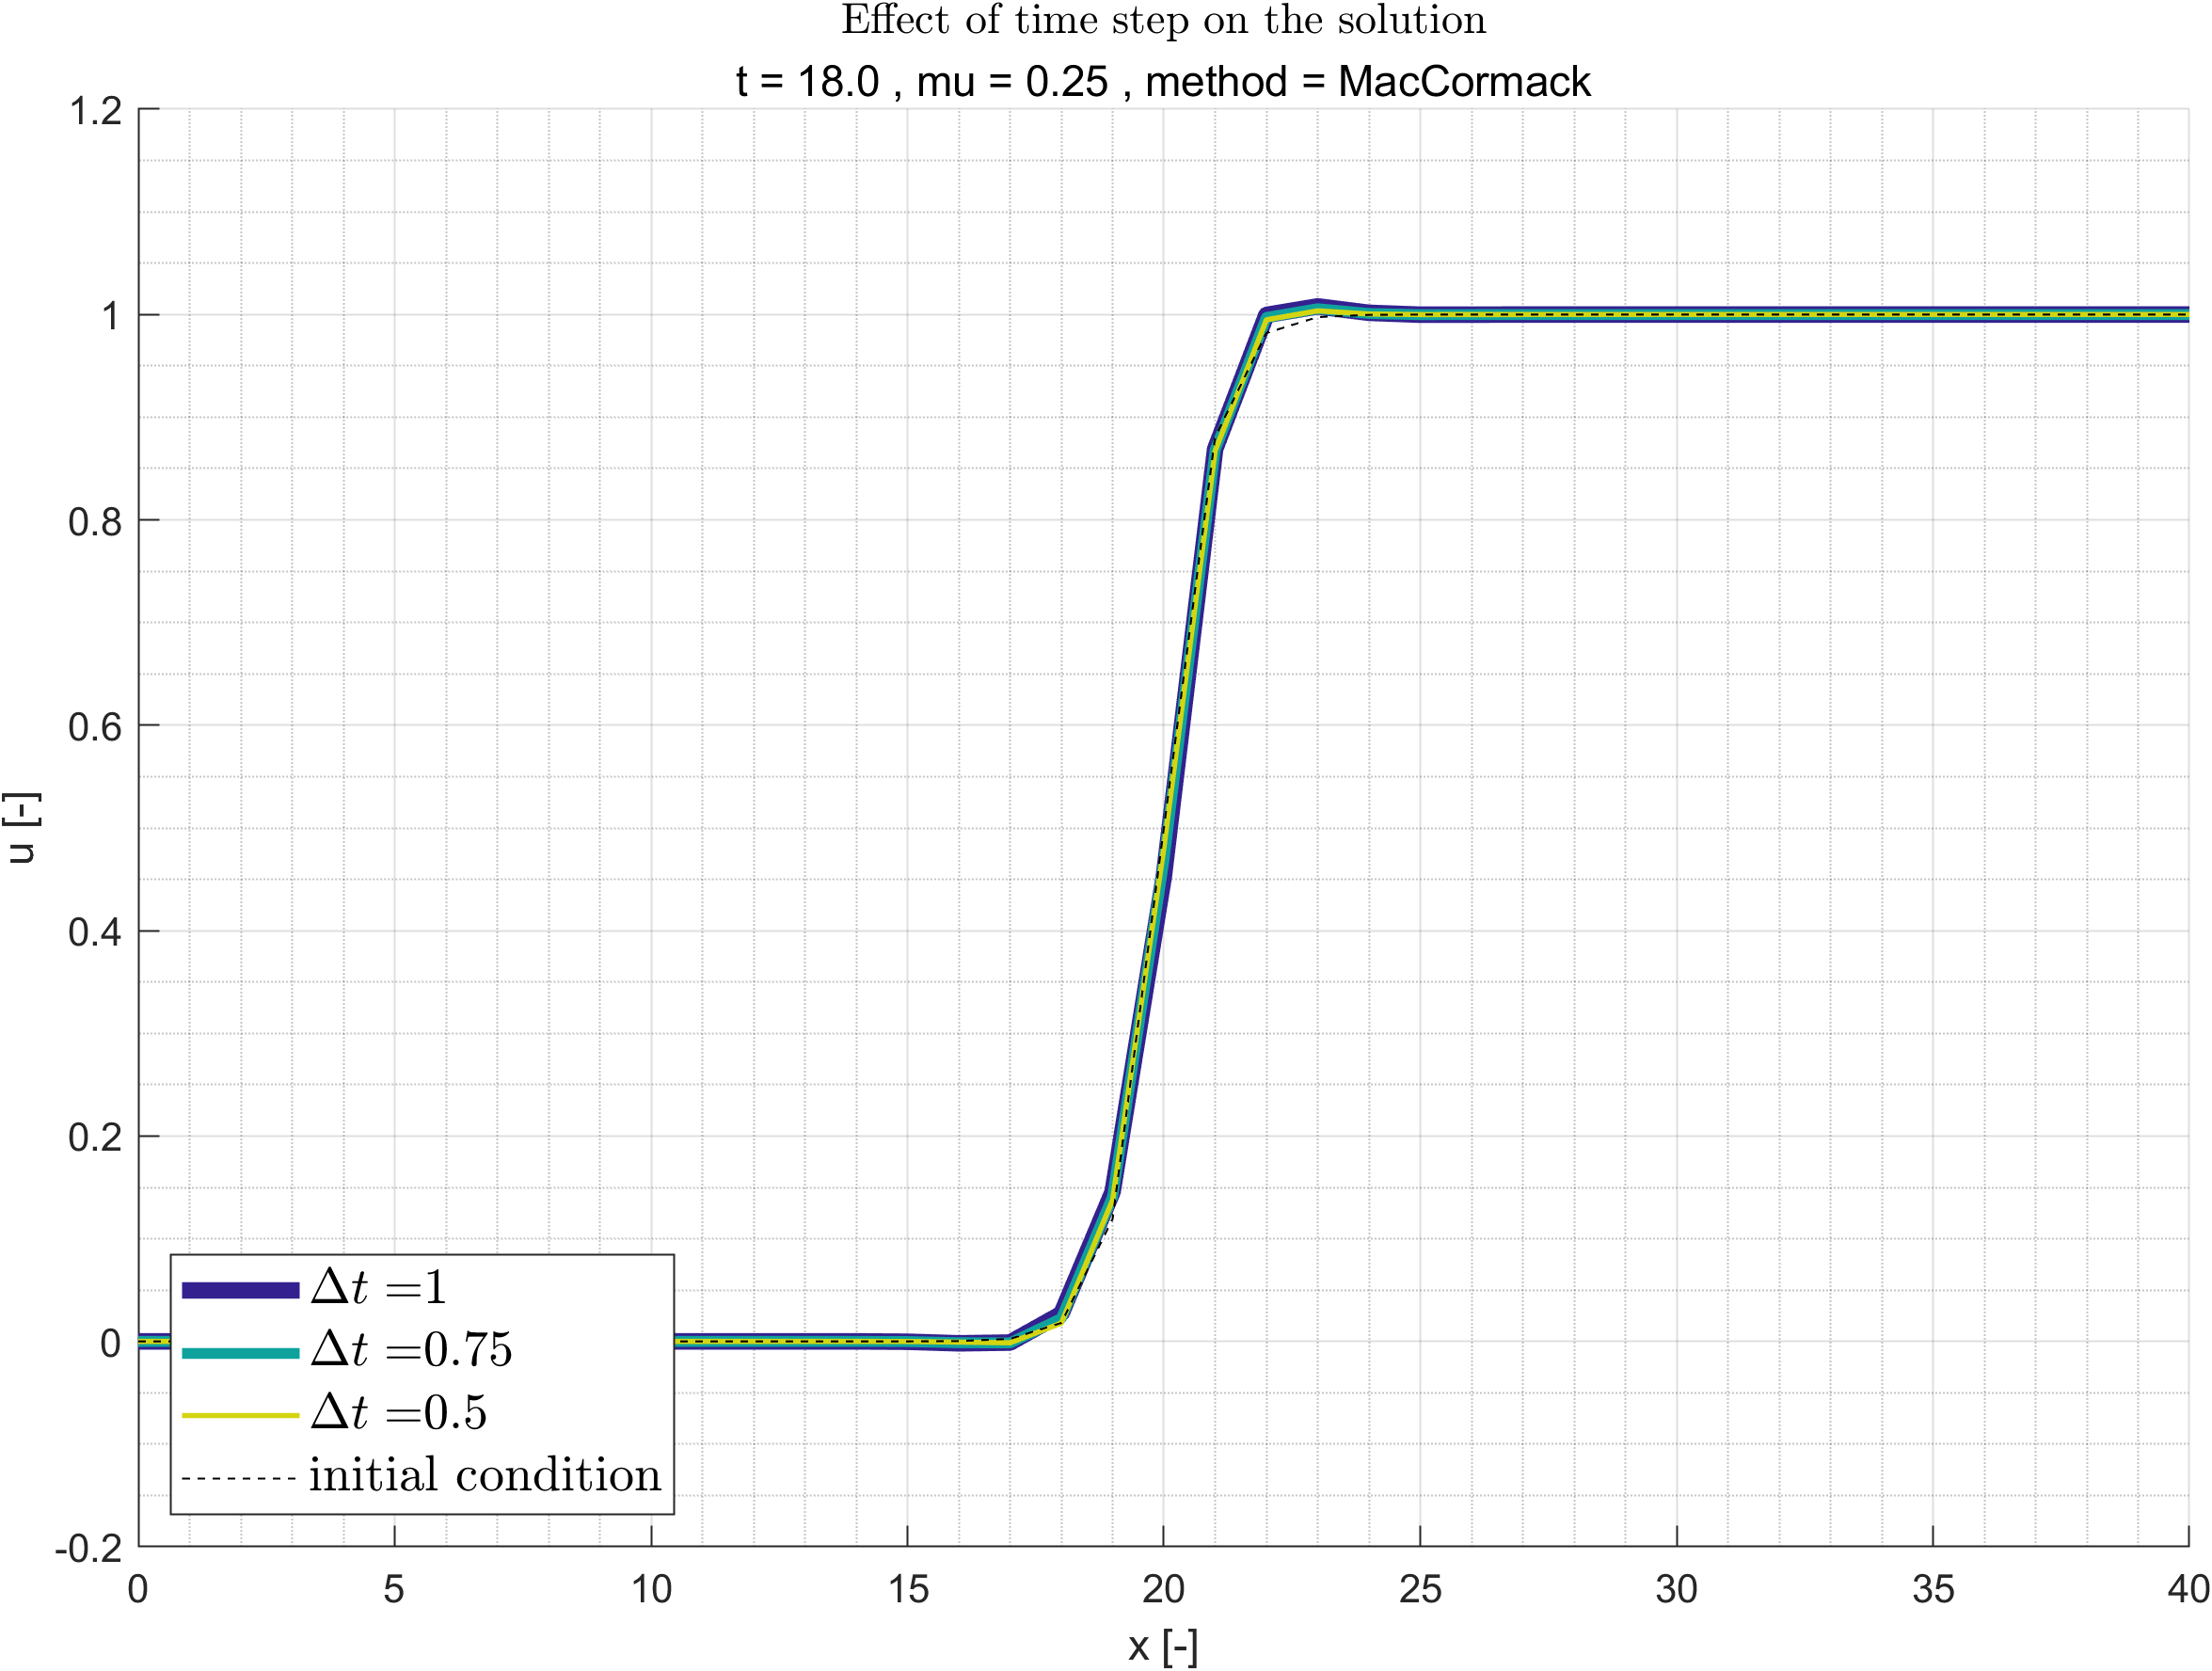
\includegraphics[width=\textwidth]{images/grap10.png}
        \caption{MacCormack $\mu=0.25$}
        \label{fig:MacCormack_general_mu0.25_A}
    \end{subfigure}
    % \hfill
    \begin{subfigure}[c]{.39\textwidth}
        \centering
        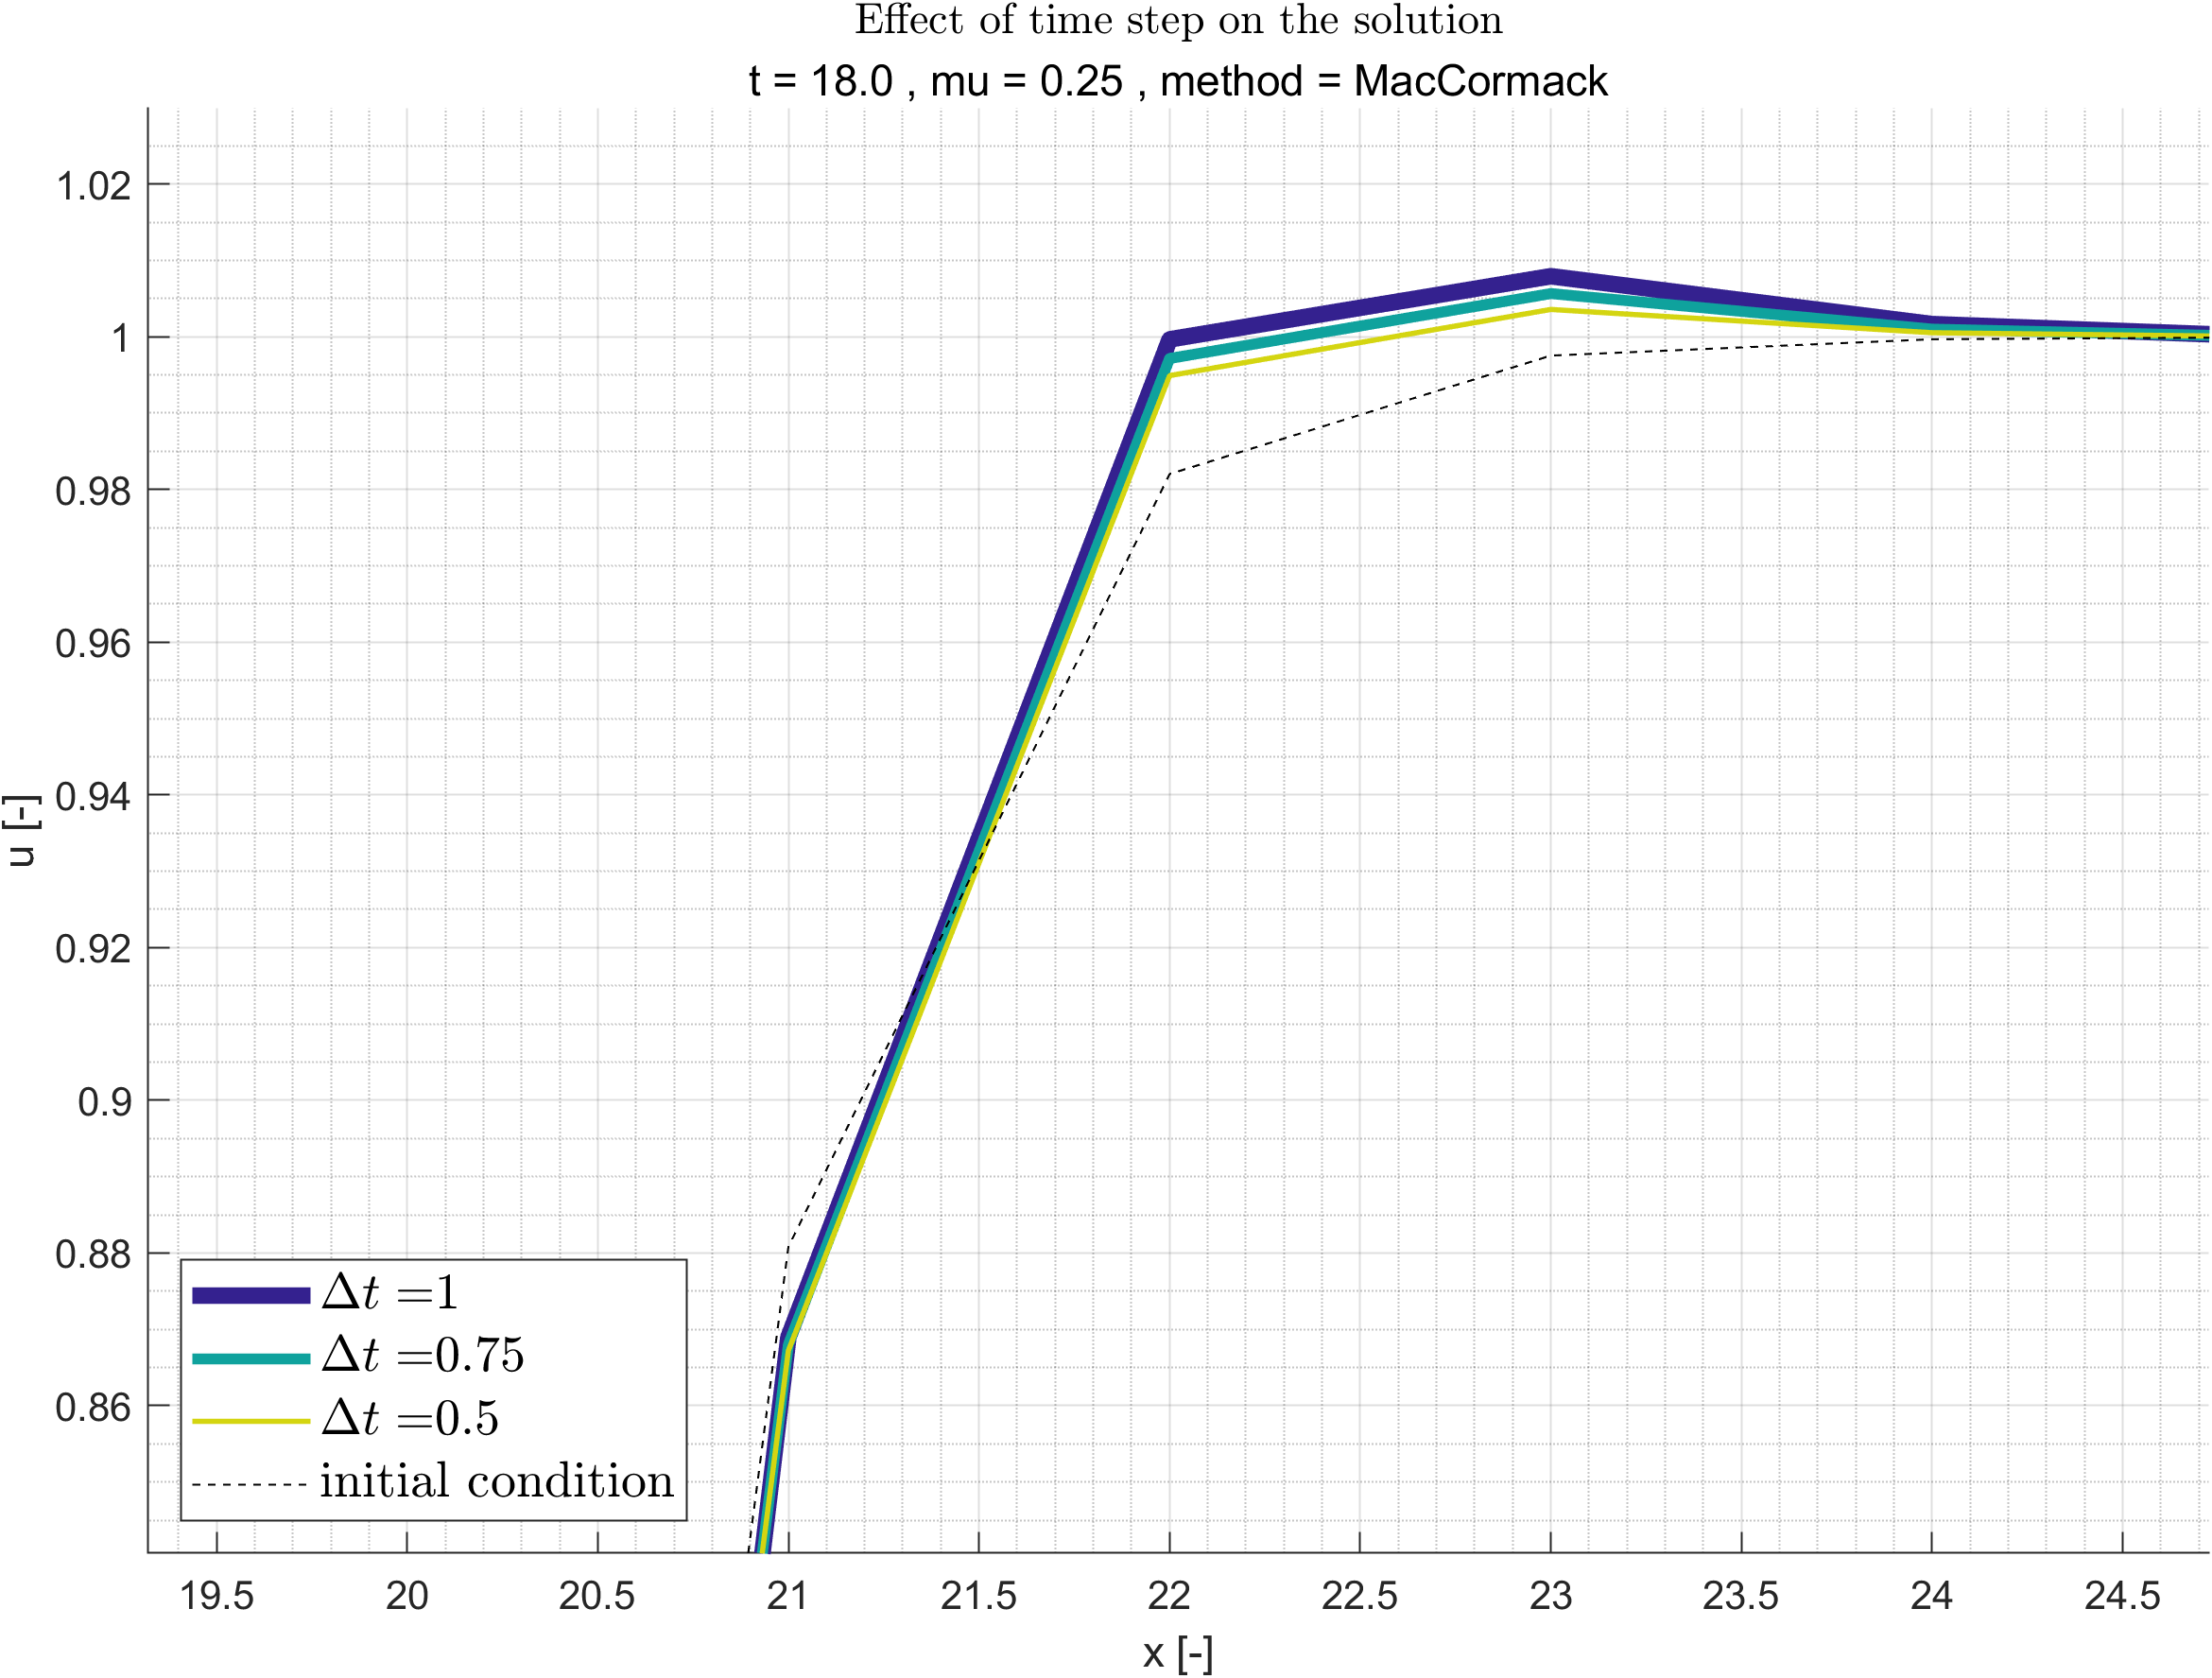
\includegraphics[width=\textwidth]{images/grap10.1.png}
        \caption{MacCormack $\mu=0.25$ - zoomed}
        \label{fig:MacCormack_general_mu0.25_B}
    \end{subfigure}
    \begin{subfigure}[c]{.39\textwidth}
        \centering
        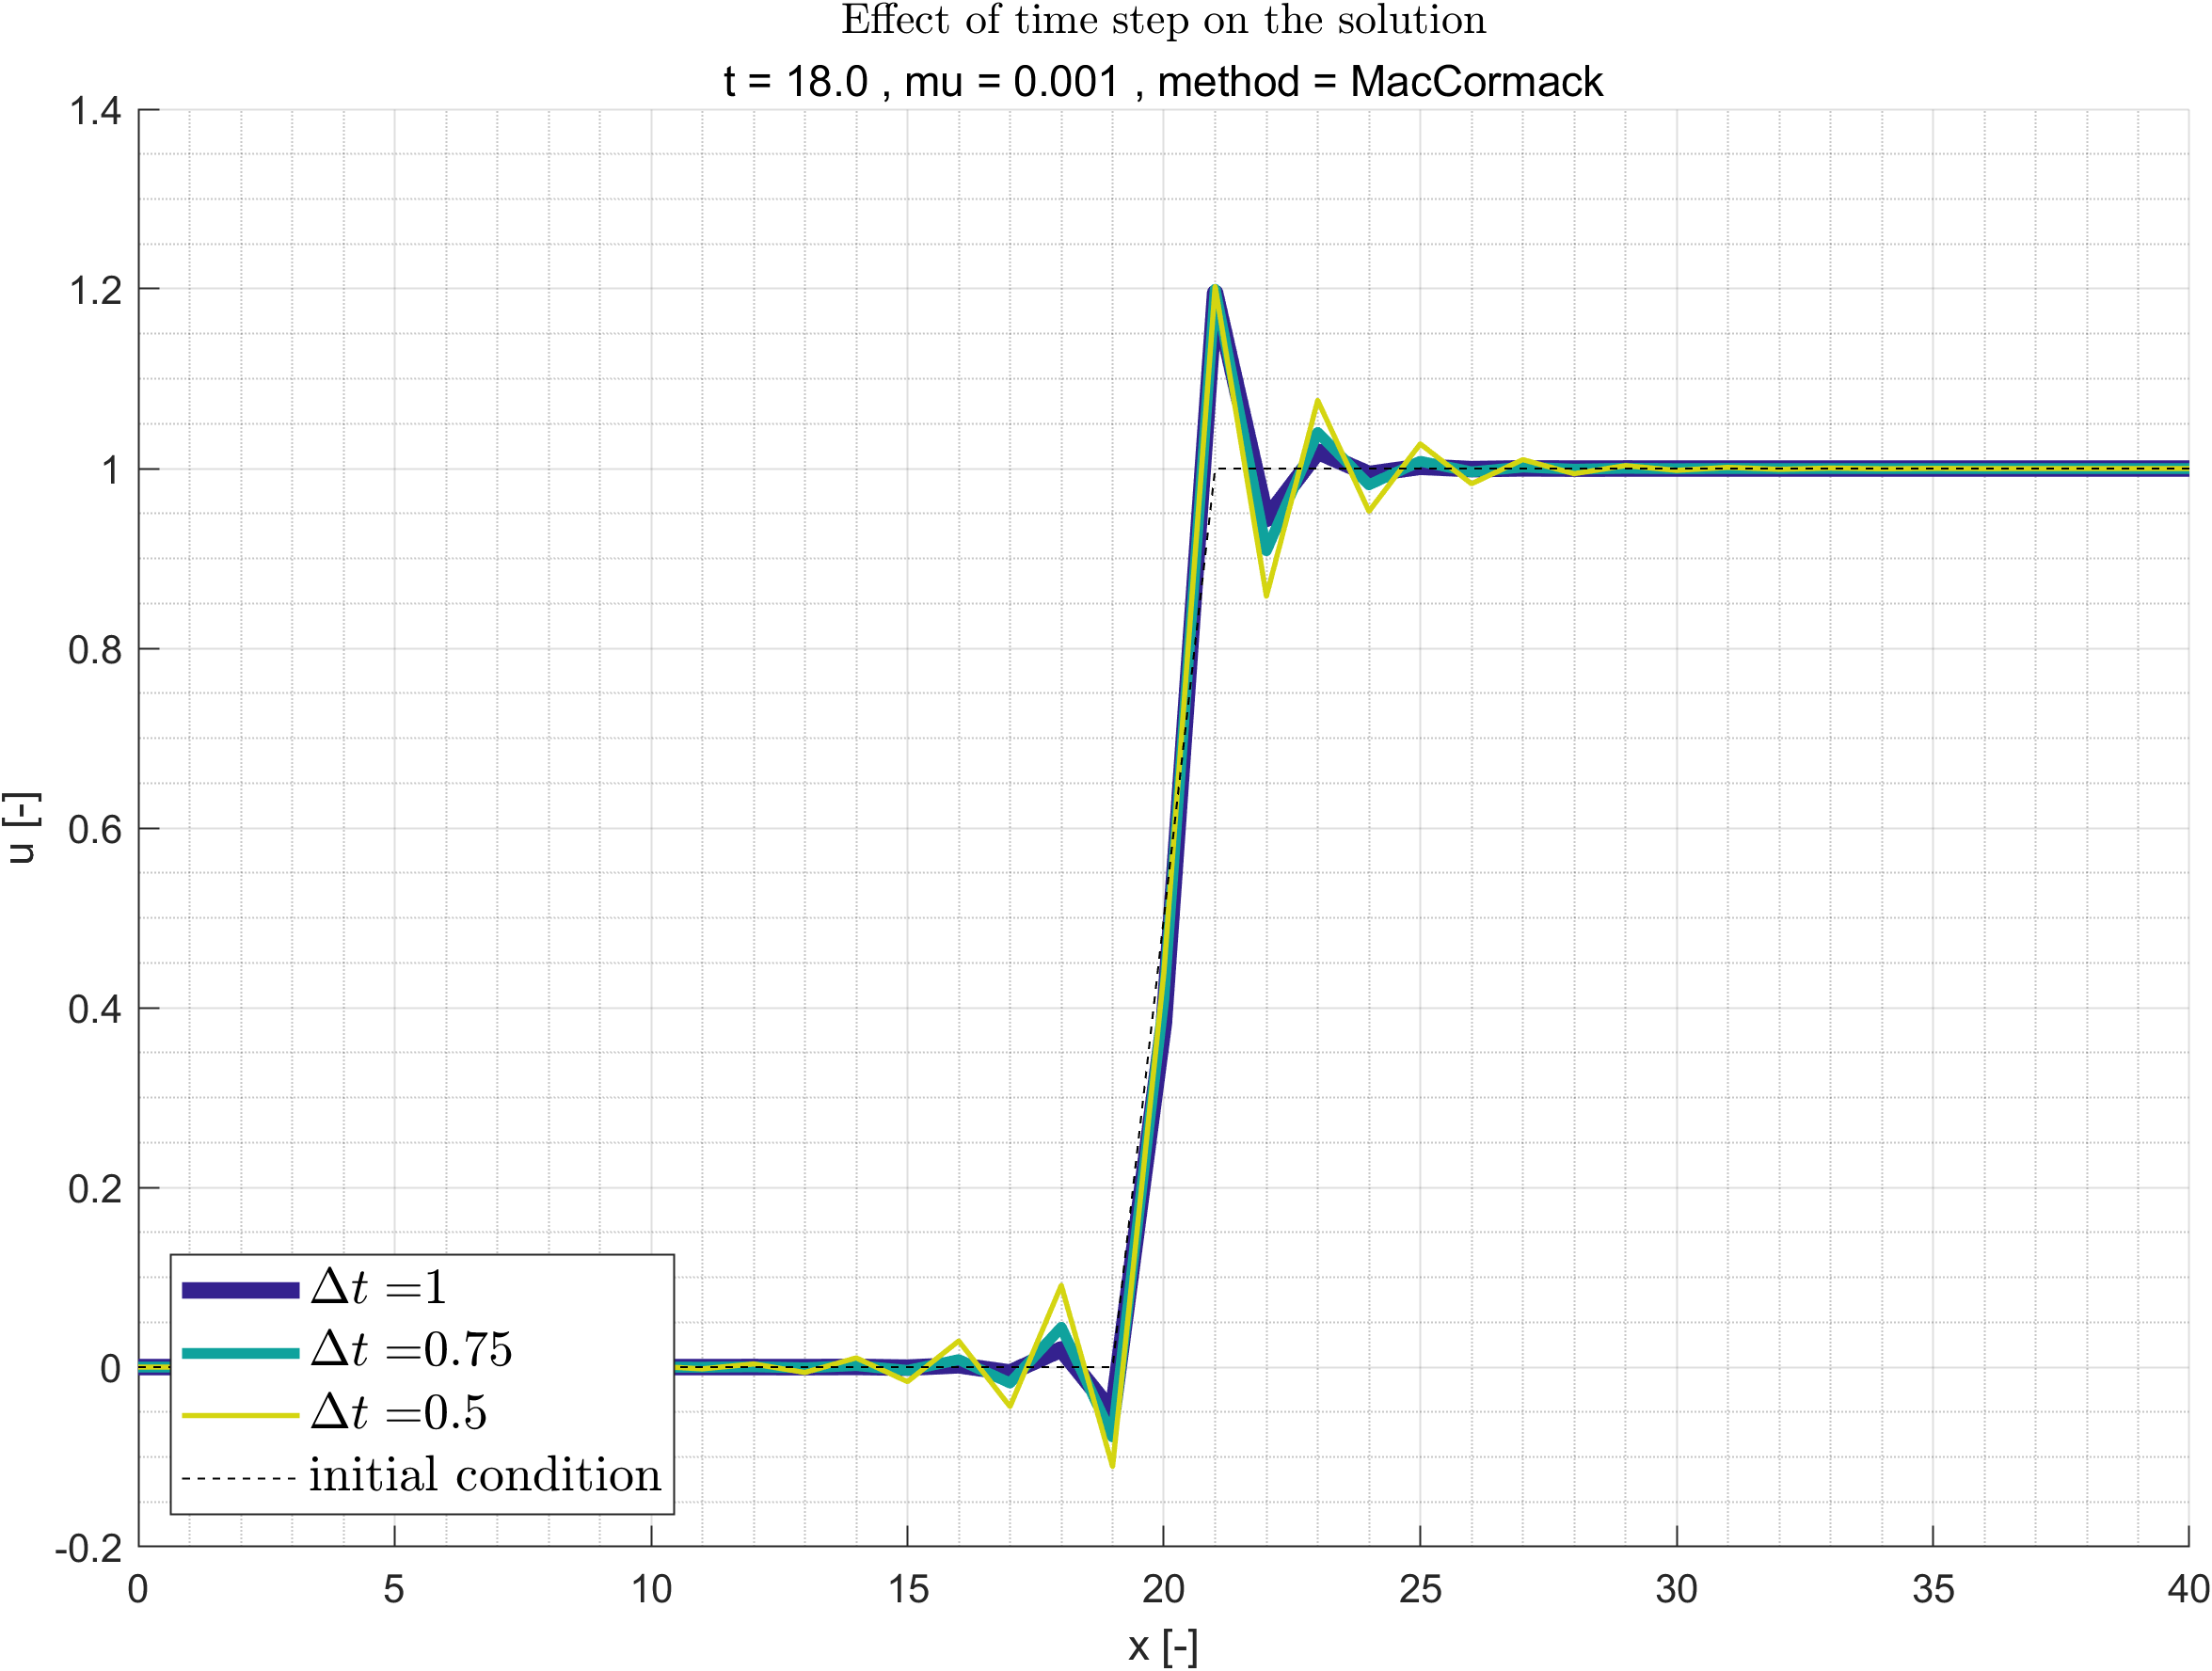
\includegraphics[width=\textwidth]{images/grap11.png}
        \caption{MacCormack $\mu=0.001$}
        \label{fig:MacCormack_general_mu0.001_A}
    \end{subfigure}
    % \hfill
    \begin{subfigure}[c]{.39\textwidth}
        \centering
        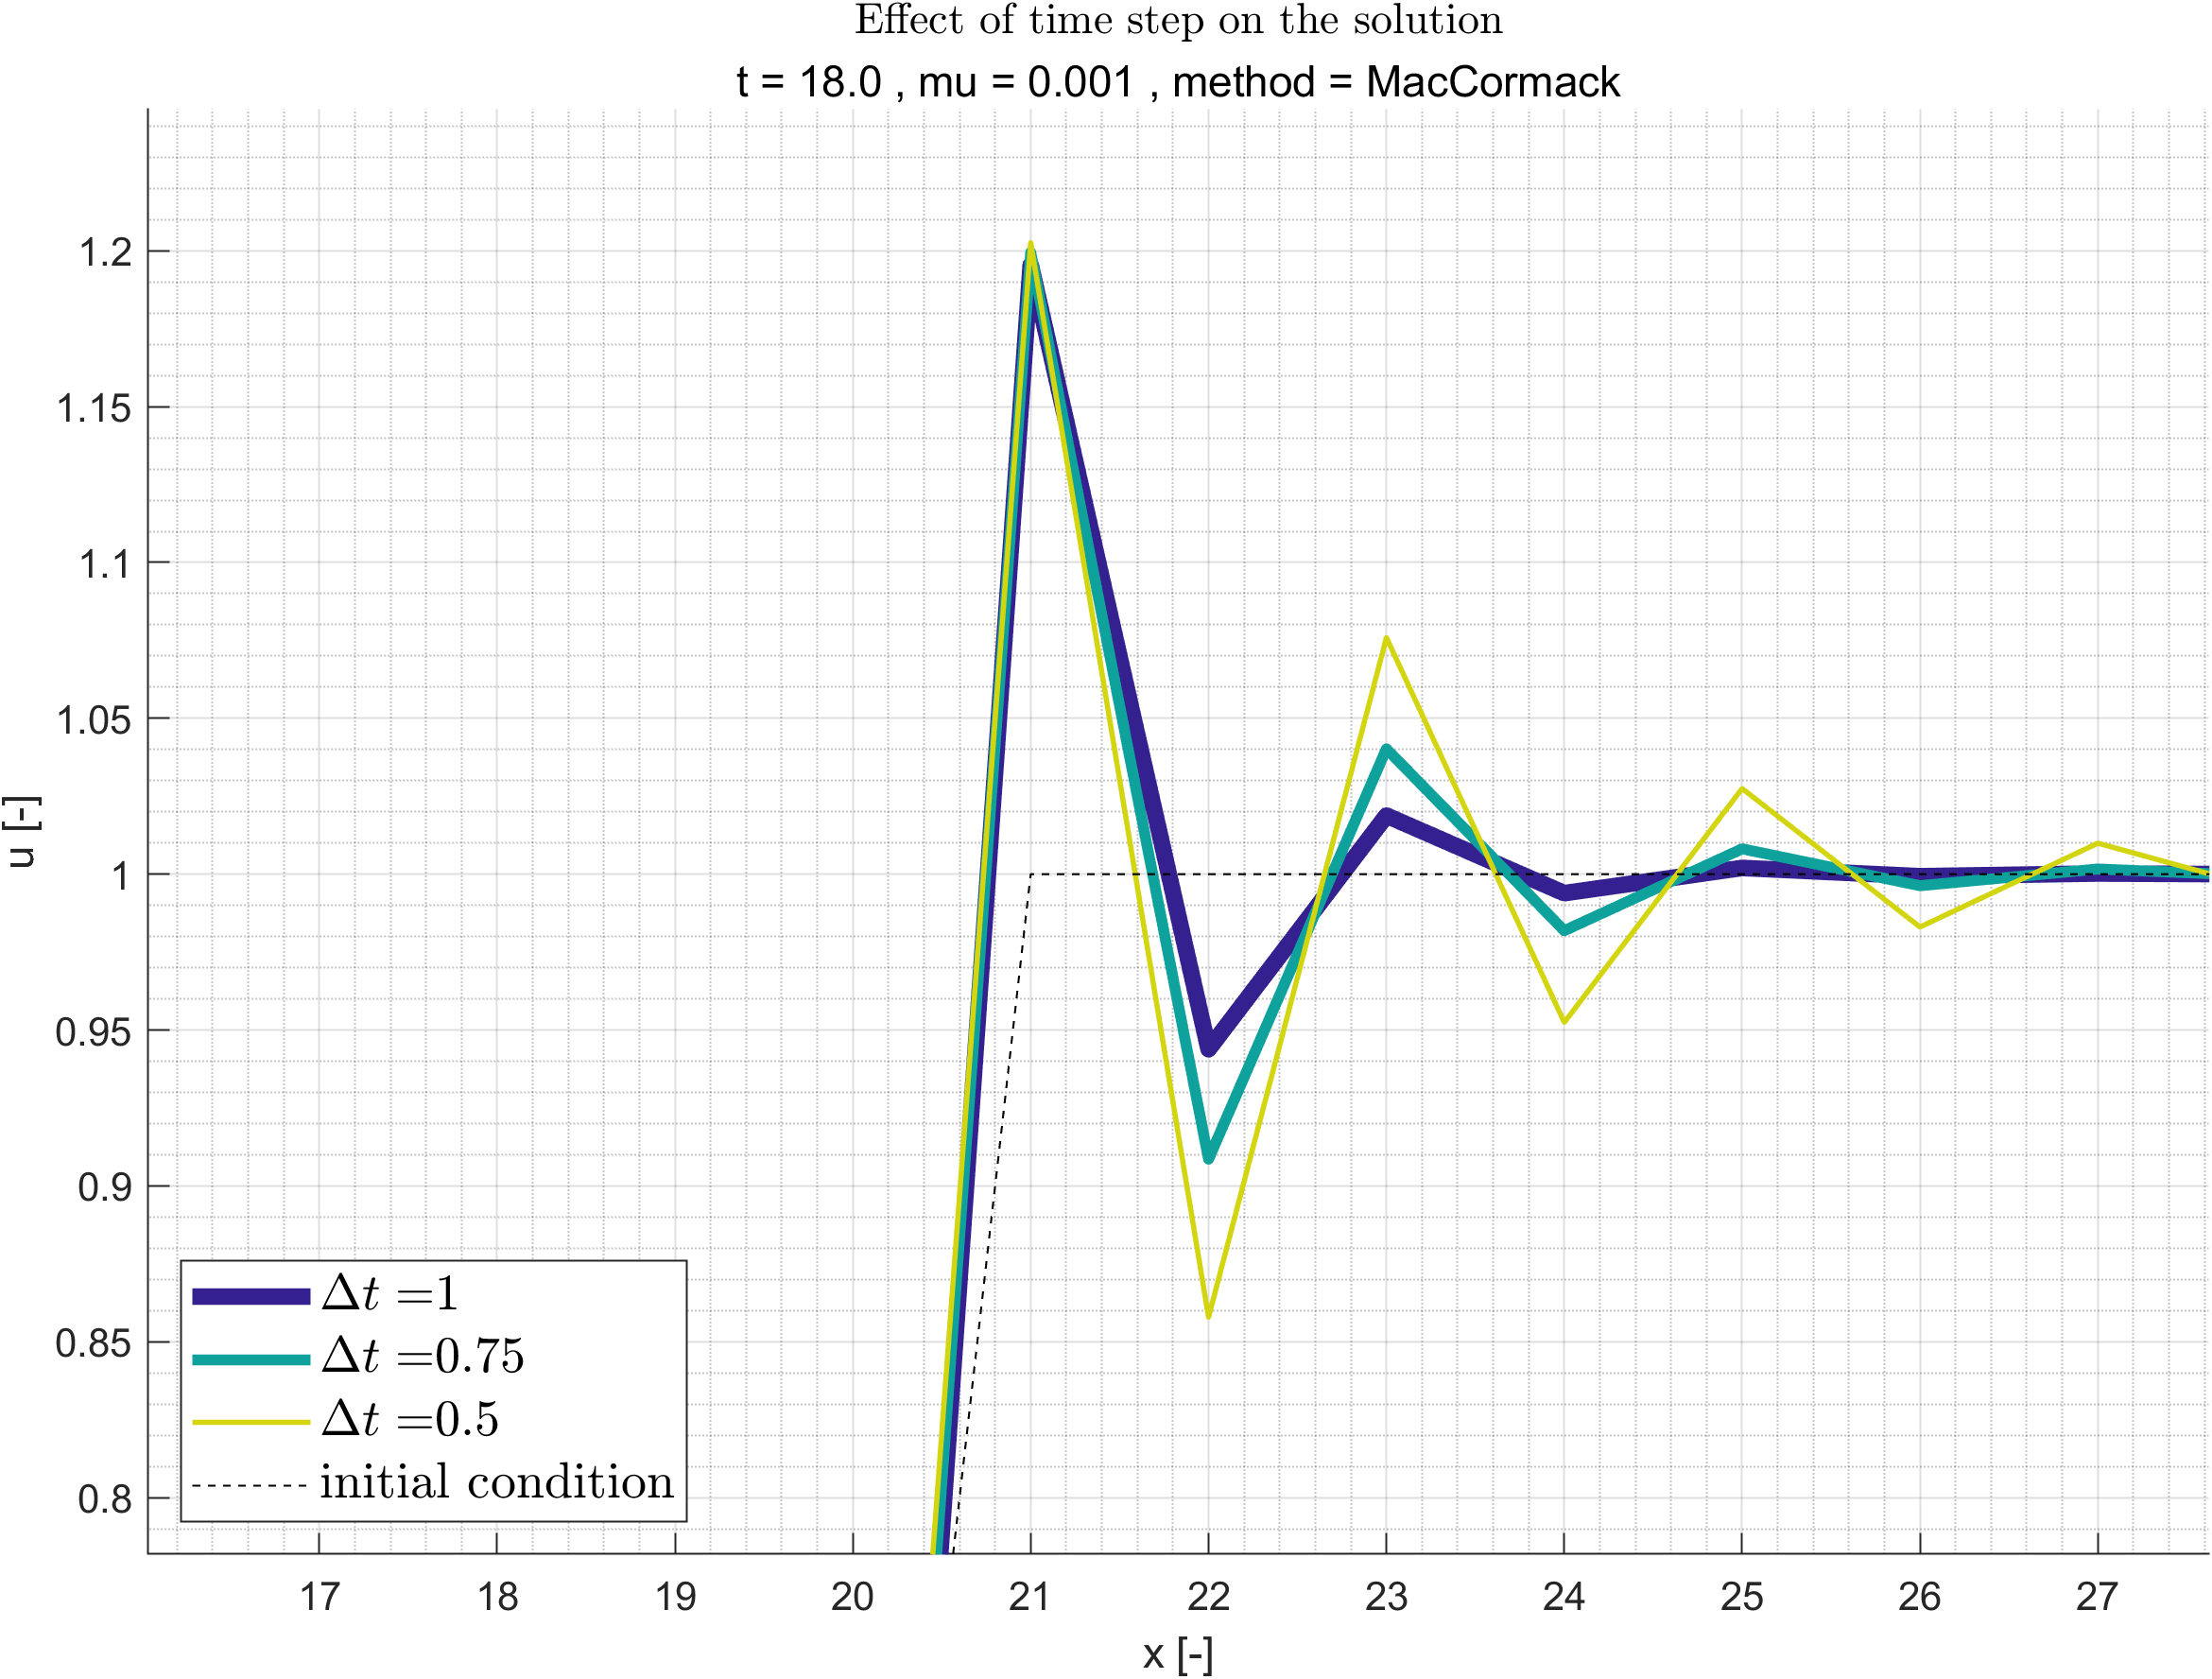
\includegraphics[width=\textwidth]{images/grap11.1.png}
        \caption{MacCormack $\mu=0.001$ - zoomed}
        \label{fig:MacCormack_general_mu0.001_B}
    \end{subfigure}
    \caption{Effect of time step on solution - MacCormack}
        \label{fig:MacCormack_general}
\end{figure}
We can see that when the viscosity is significant, the time step has near to no effect on the solution. When the viscosity is negligible, the time step has a significant effect on the solution, and as the time step increases the oscillations decrease and the solution dampens.
\newpage

\subsection{Beam and Warming}
Beam and Warming inroduced the Delta form and their method is more efficient:
\begin{equation}
    \begin{array}{c}
        \displaystyle\left(I+\theta\left(\Delta t\frac{D_0A_i^n}{2\Delta x}-\frac{\Delta t\mu}{\left(\Delta x\right)^2}\delta^2\right)\right)\Delta u_i^n=\underbrace{-\Delta t\frac{F_{i+1}^n-F_{i-1}^n}{2\Delta x}+\Delta t\mu\frac{u^n_{i+1}-2u^n_i+u^n_{i-1}}{\left(\Delta x\right)^2}}_{\displaystyle\mathrm{RHS}_i^n} \\
        \left\{\begin{array}{ll}
            \theta=1 & \mathrm{first\ order} \\
            \theta=0.5 & \mathrm{second\ order}
        \end{array}\right.
    \end{array}
\end{equation}
Deriving the matrix to invert:
\begin{align*}
    \displaystyle\left(I+\theta\Delta t\frac{D_0A_i^n}{2\Delta x}\right)\Delta u_i^n-\theta\frac{\Delta t\mu}{\left(\Delta x\right)^2}\delta^2\Delta u^n_i&=\mathrm{RHS}^n_i\\
    \displaystyle\left(I+\theta\Delta t\frac{D_0A_i^n}{2\Delta x}\right)\Delta u_i^n-\theta\frac{\Delta t\mu}{\left(\Delta x\right)^2}\left(\Delta u^n_{i+1}-2\Delta u^n_i+\Delta u^n_{i-1}\right)&=\mathrm{RHS_i^n} \\
    \displaystyle\Delta u_i^n+\theta\frac{\Delta t}{2\Delta x}\left(A_{i+1}^n\Delta u_{i+1}^n-A_{i-1}^n\Delta u_{i-1}^n\right)-\theta\frac{\Delta t\mu}{\left(\Delta x\right)^2}\left(\Delta u^n_{i+1}-2\Delta u^n_i+\Delta u^n_{i-1}\right)&=\mathrm{RHS_i^n} \\
    A_i\Delta u^n_{i-1}+B_i\Delta u^n_i+C_i\Delta u^n_{i+1}&=D_i
\end{align*}
\begin{equation*}
    \Downarrow
\end{equation*}
\begin{equation}
    \begin{array}{lcl}
        A'_i &=& \displaystyle-\theta\frac{\mu\Delta t}{\left(\Delta x\right)^2}-\theta\frac{\Delta t}{2\Delta x}A_{i-1}^n\\
        B'_i &=& \displaystyle1+2\theta\frac{\mu\Delta t}{\left(\Delta x\right)^2}\\
        C'_i &=& \displaystyle-\theta\frac{\mu\Delta t}{\left(\Delta x\right)^2}+\theta\frac{\Delta t}{2\Delta x}A_{i+1}^n\\
        D'_i &=& RHS_i^n
    \end{array}
\end{equation}
and advancing the solution with:
\begin{equation}
    u_i^{n+1}=u_i^n+\Delta u_i^n
\end{equation}
In order to calculate $\Delta u^n_i$ it is needed to invert matrix as follows:
\begin{equation}
    \begin{pmatrix}
        B'_1 & C'_1 & 0 & \cdots & \cdots & \cdots & 0 \\
        A'_2 & B'_2 & C'_2 & 0 & \cdots & \cdots & 0 \\
        0 & \ddots & \ddots & \ddots & 0 & \cdots & 0 \\
        0 & 0 & A'_i & B'_i & C'_i & 0 & 0 \\
        0 & \cdots & 0 & \ddots & \ddots & \ddots & 0 \\
        0 & \cdots & \cdots & 0 & A'_{N-1} & B'_{N-1} & C'_{N-1} \\
        0 & 0 & \cdots & \cdots & 0 & A'_{N} &B'_{N}
    \end{pmatrix}
    \begin{pmatrix}
        \Delta u_1^n\\
        \Delta u_2^n\\
        \cdots\\
        \cdots\\
        \cdots\\
        \Delta u_{N-1}^n\\
        \Delta u_{N}^n
    \end{pmatrix}
    =
    \begin{pmatrix}
        D'_1\\
        D'_2\\
        \cdots\\
        \cdots\\
        \cdots\\
        D'_{N-1}\\
        D'_{N}
    \end{pmatrix}
\end{equation}
The Beam and Warming method is extremely dispersive and therefore artiricial viscosity must be explicitly added. Beam and Warming used the following artificial viscosity term:
\begin{equation}
    \begin{matrix}
        \displaystyle-\frac{w}{8}\left(u^n_{i+2}-4u^n_{i+1}+6u^n_i-4u^n_{i-1}+u^n_{i-2}\right) && 0<w\le1
    \end{matrix}
\end{equation}
which can be added to the RHS with no change in accuracy.
\subsubsection{Effect of Time Step}
\begin{figure}[H]
    \centering
    \begin{subfigure}[c]{.38\textwidth}
        \centering
        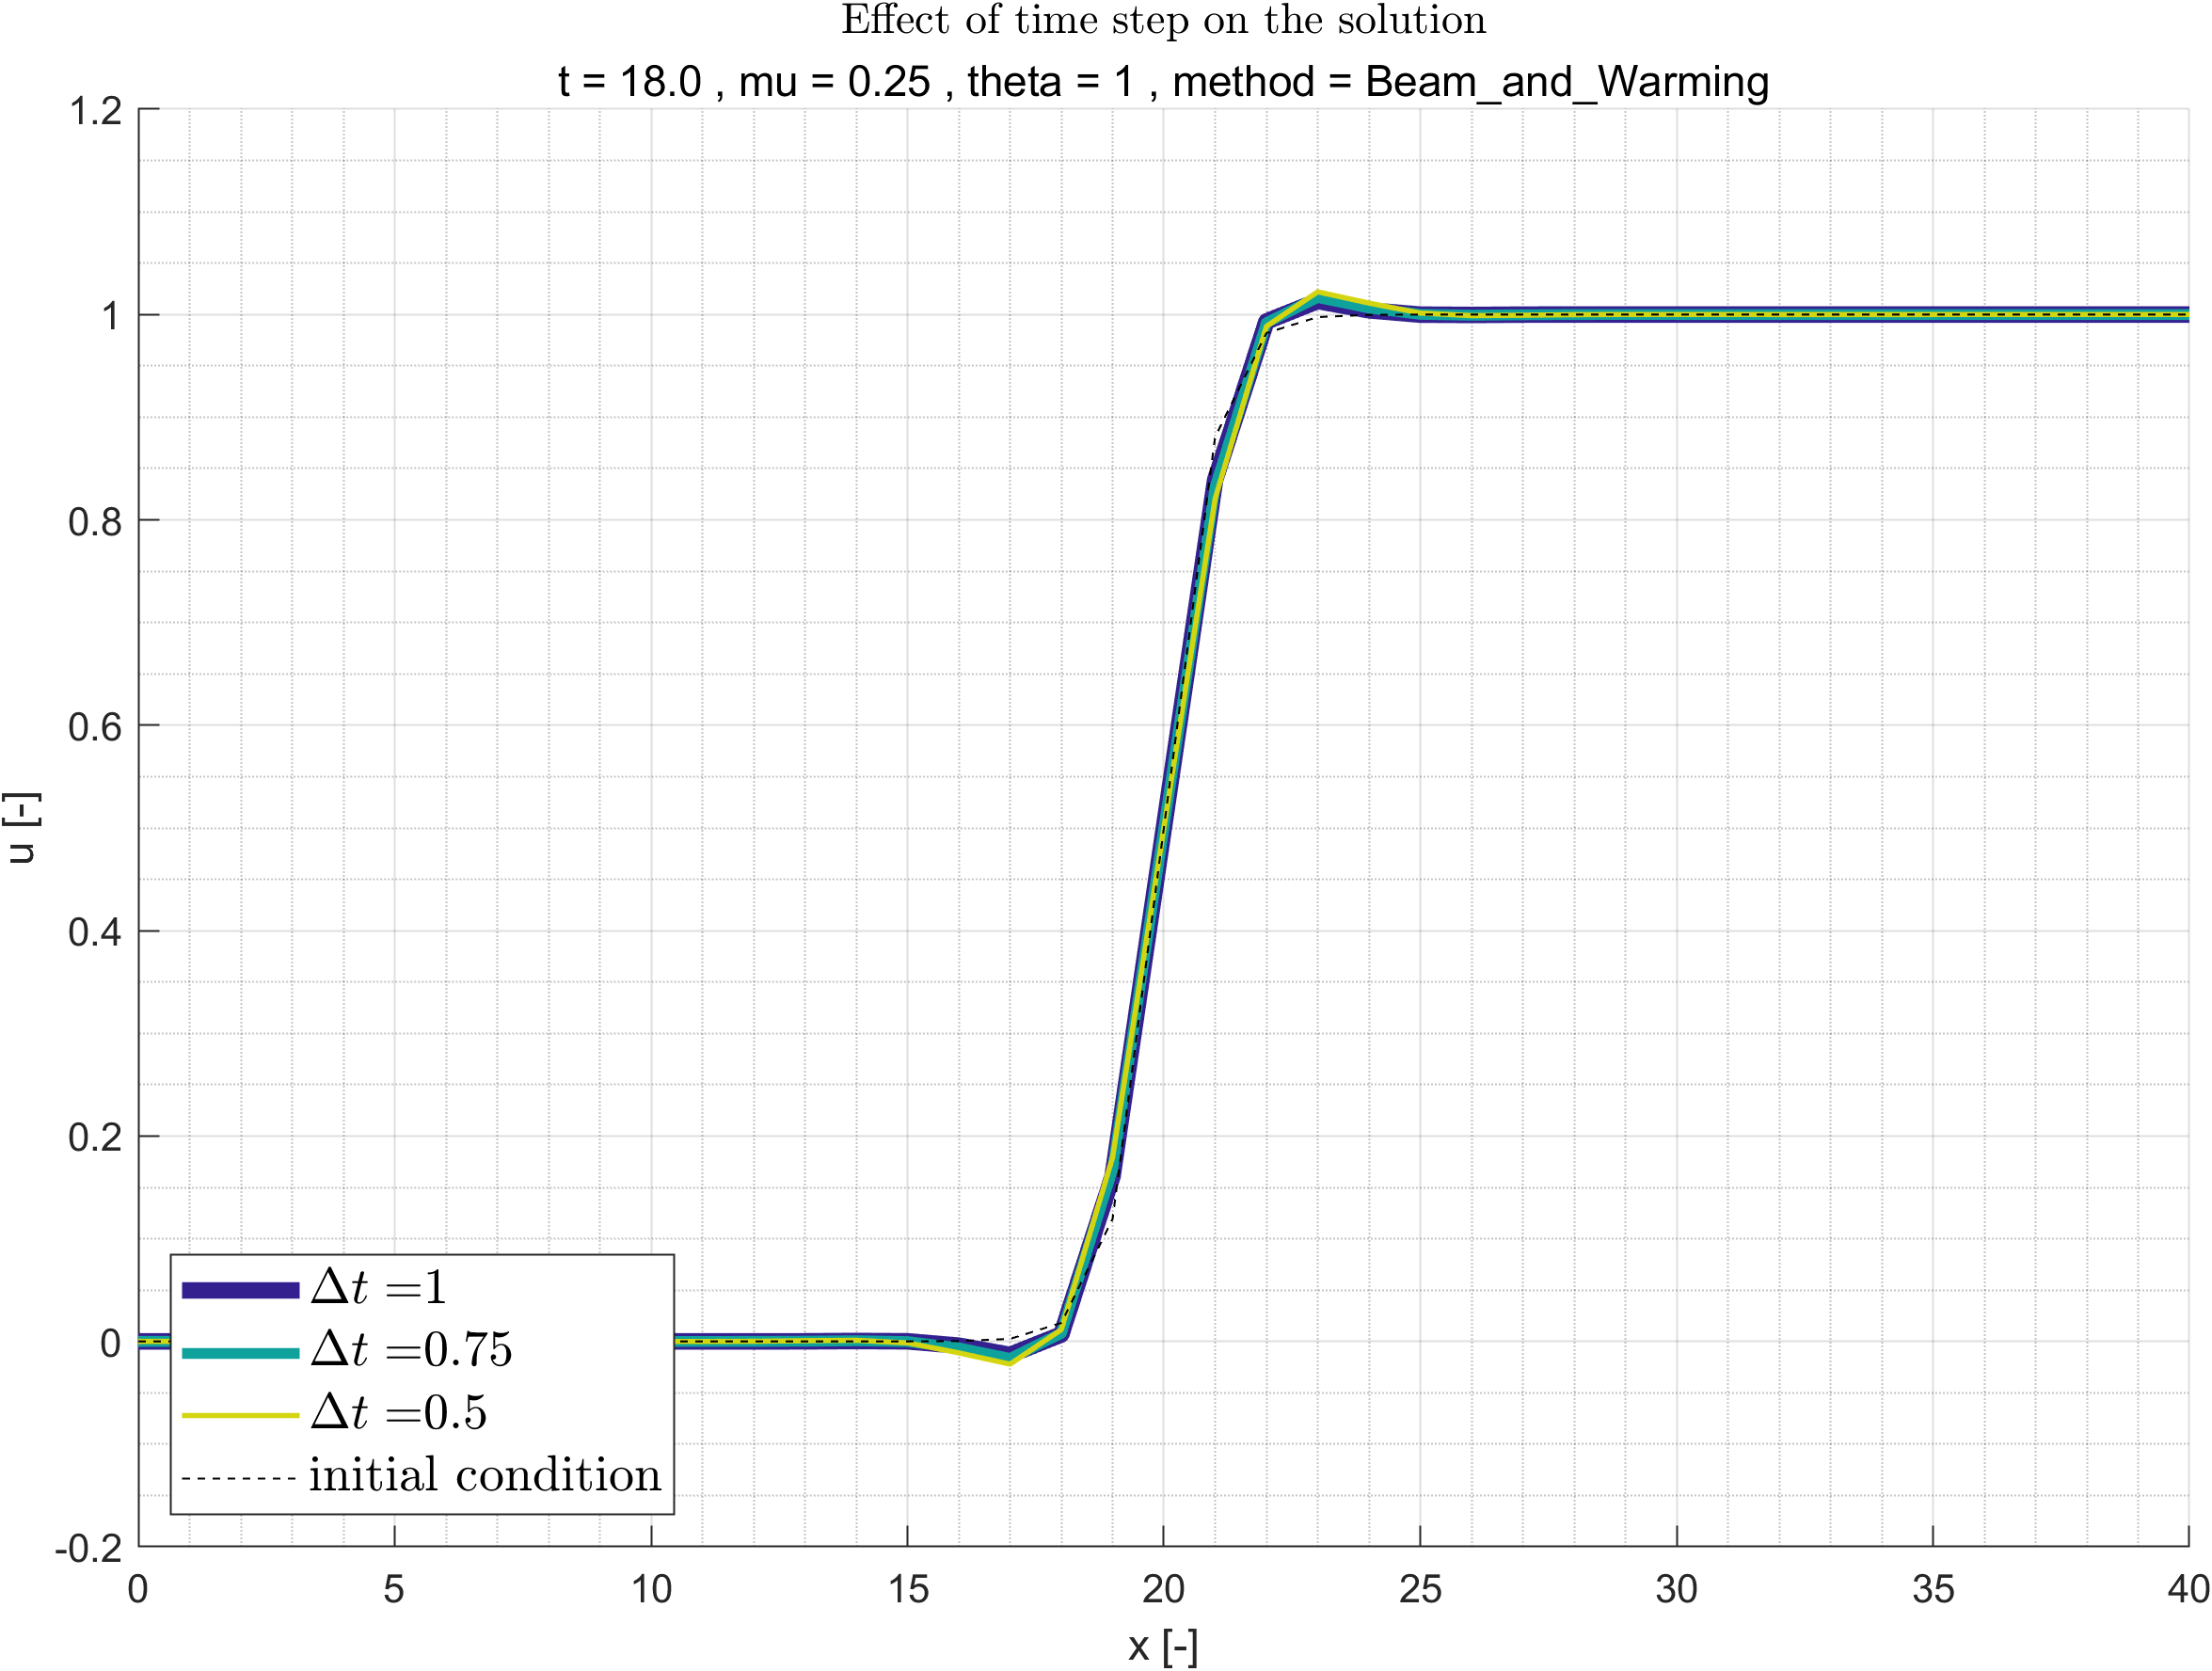
\includegraphics[width=\textwidth]{images/grap12.png}
        \caption{Beam $\&$ Warming $\mu=0.25,\ \theta=1$}
        \label{fig:Beam & Warming_general_mu0.25_theta1_A_diff_time}
    \end{subfigure}
    % \hfill
    \begin{subfigure}[c]{.38\textwidth}
        \centering
        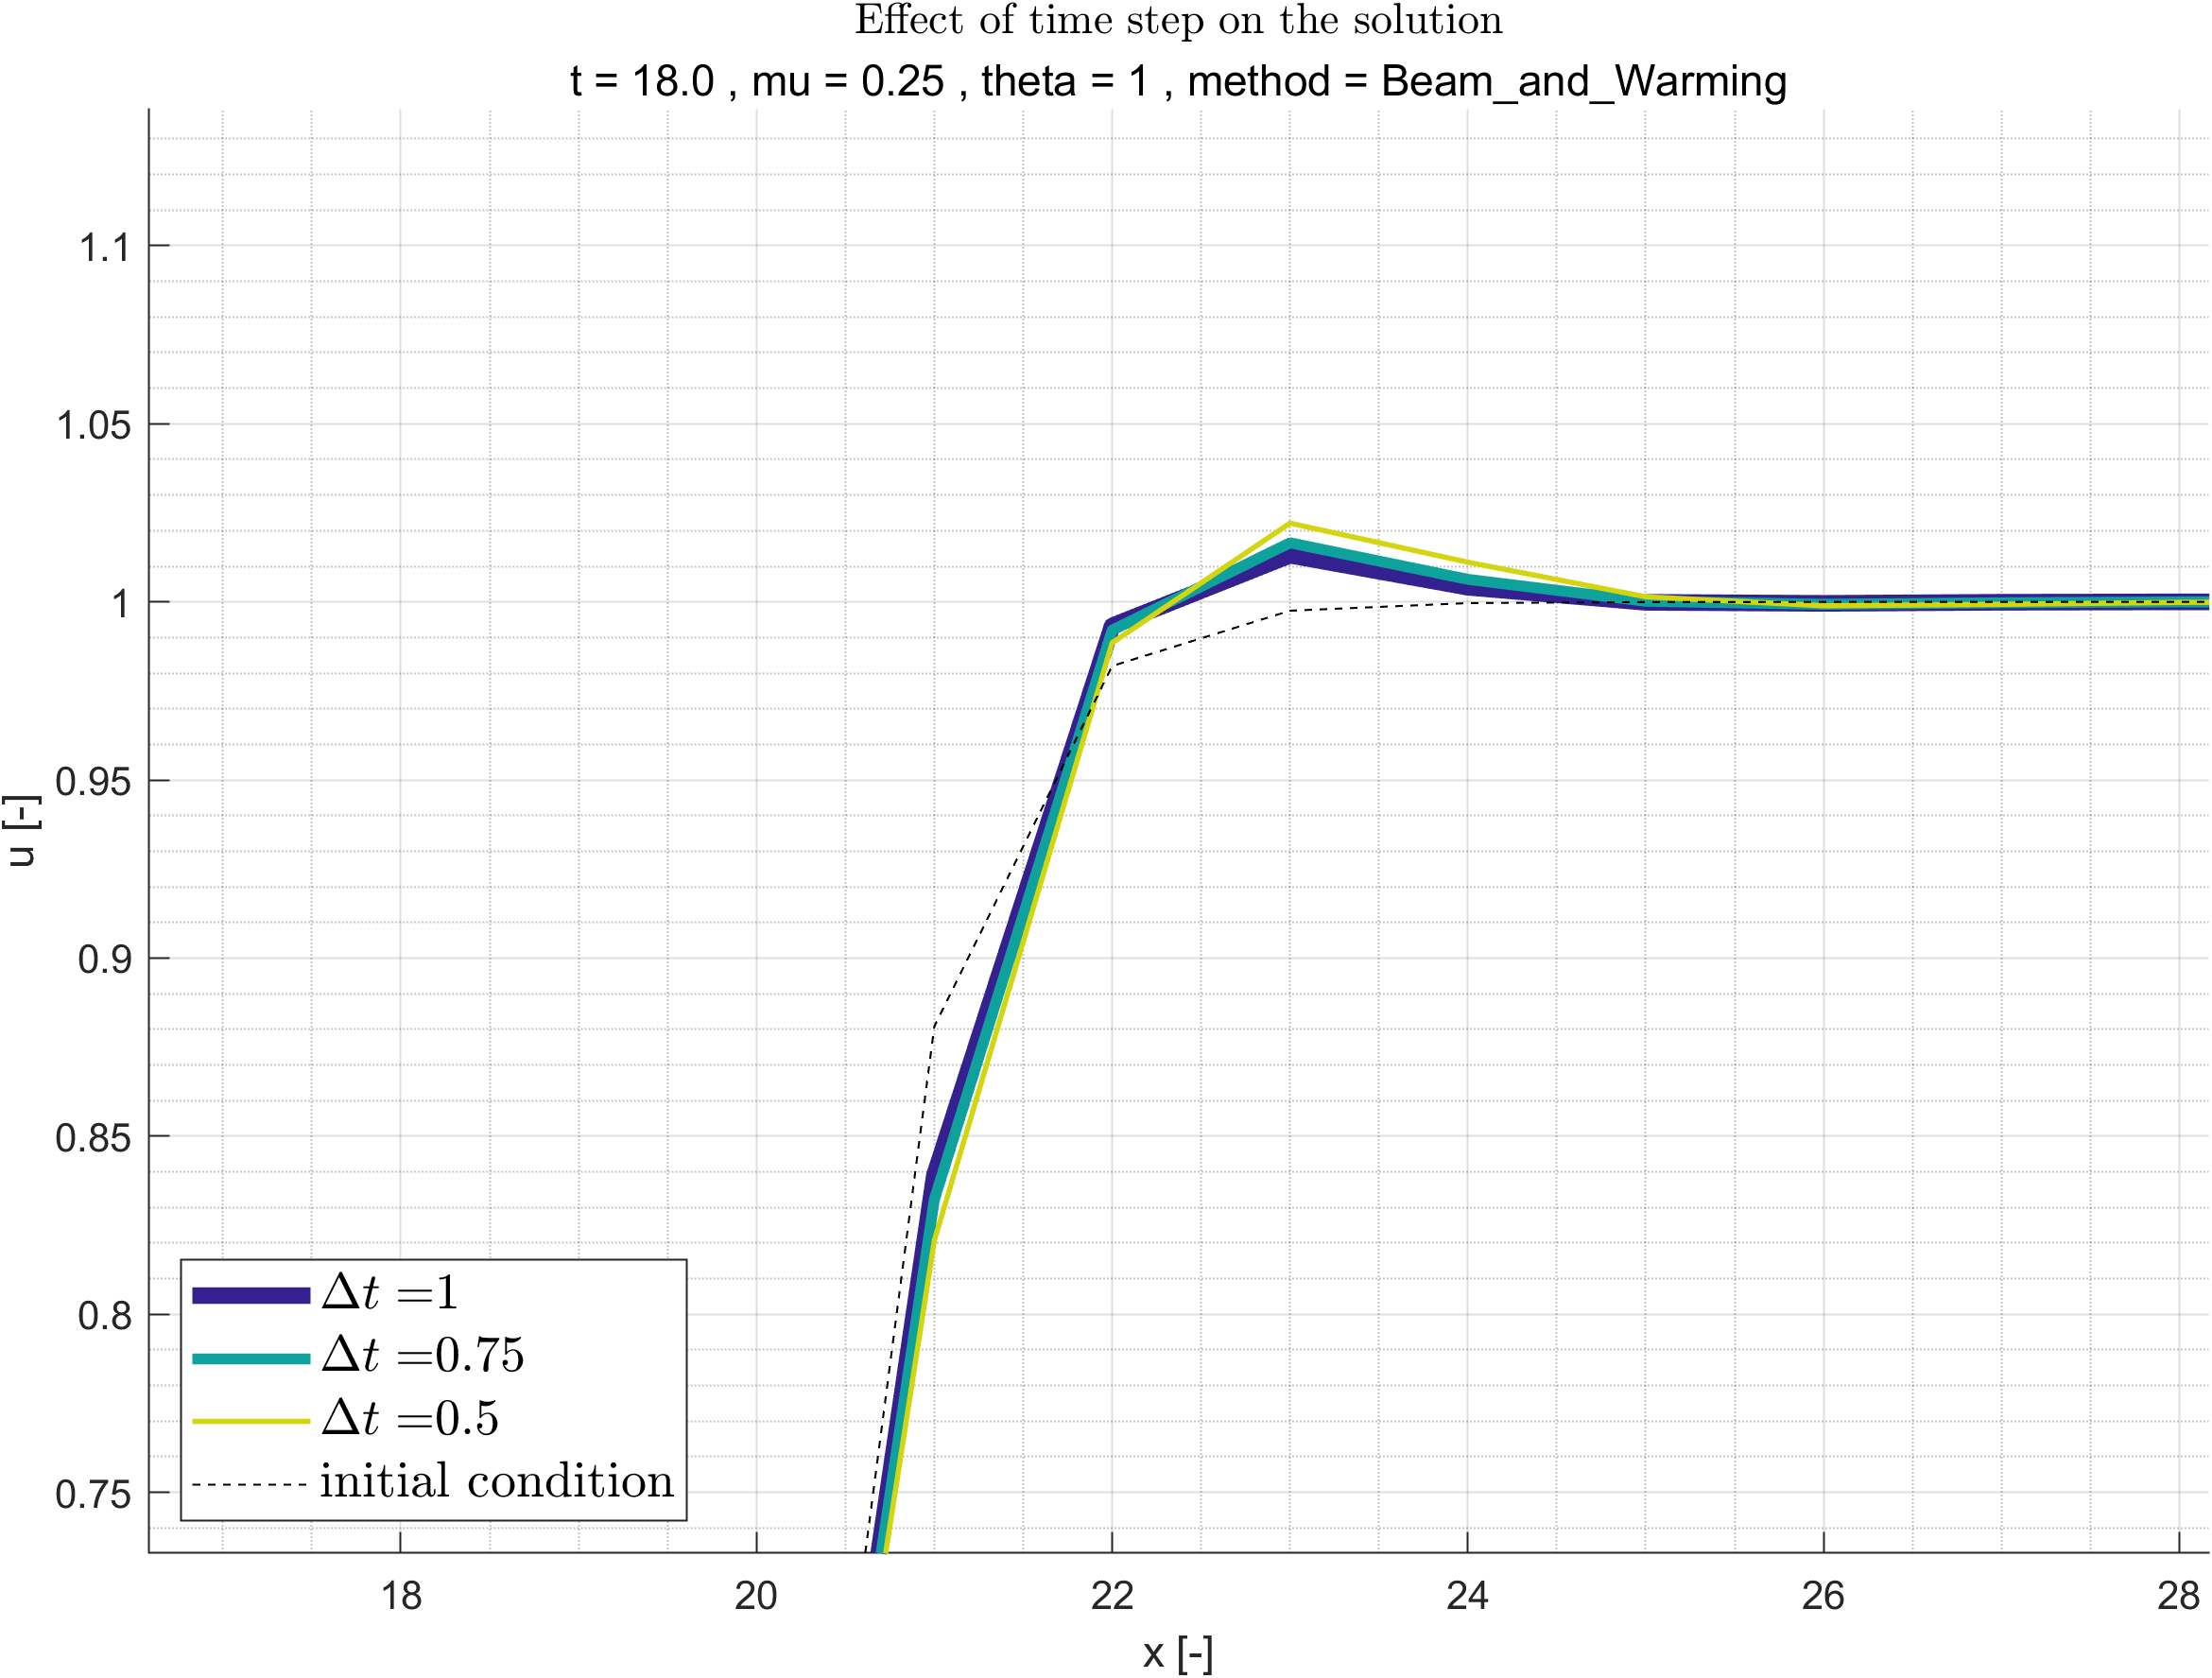
\includegraphics[width=\textwidth]{images/grap12.1.png}
        \caption{Beam $\&$ Warming $\mu=0.25,\ \theta=1$ - zoomed}
        \label{fig:Beam & Warming_general_mu0.25_theta1_B_diff_time}
    \end{subfigure}
    \begin{subfigure}[c]{.38\textwidth}
        \centering
        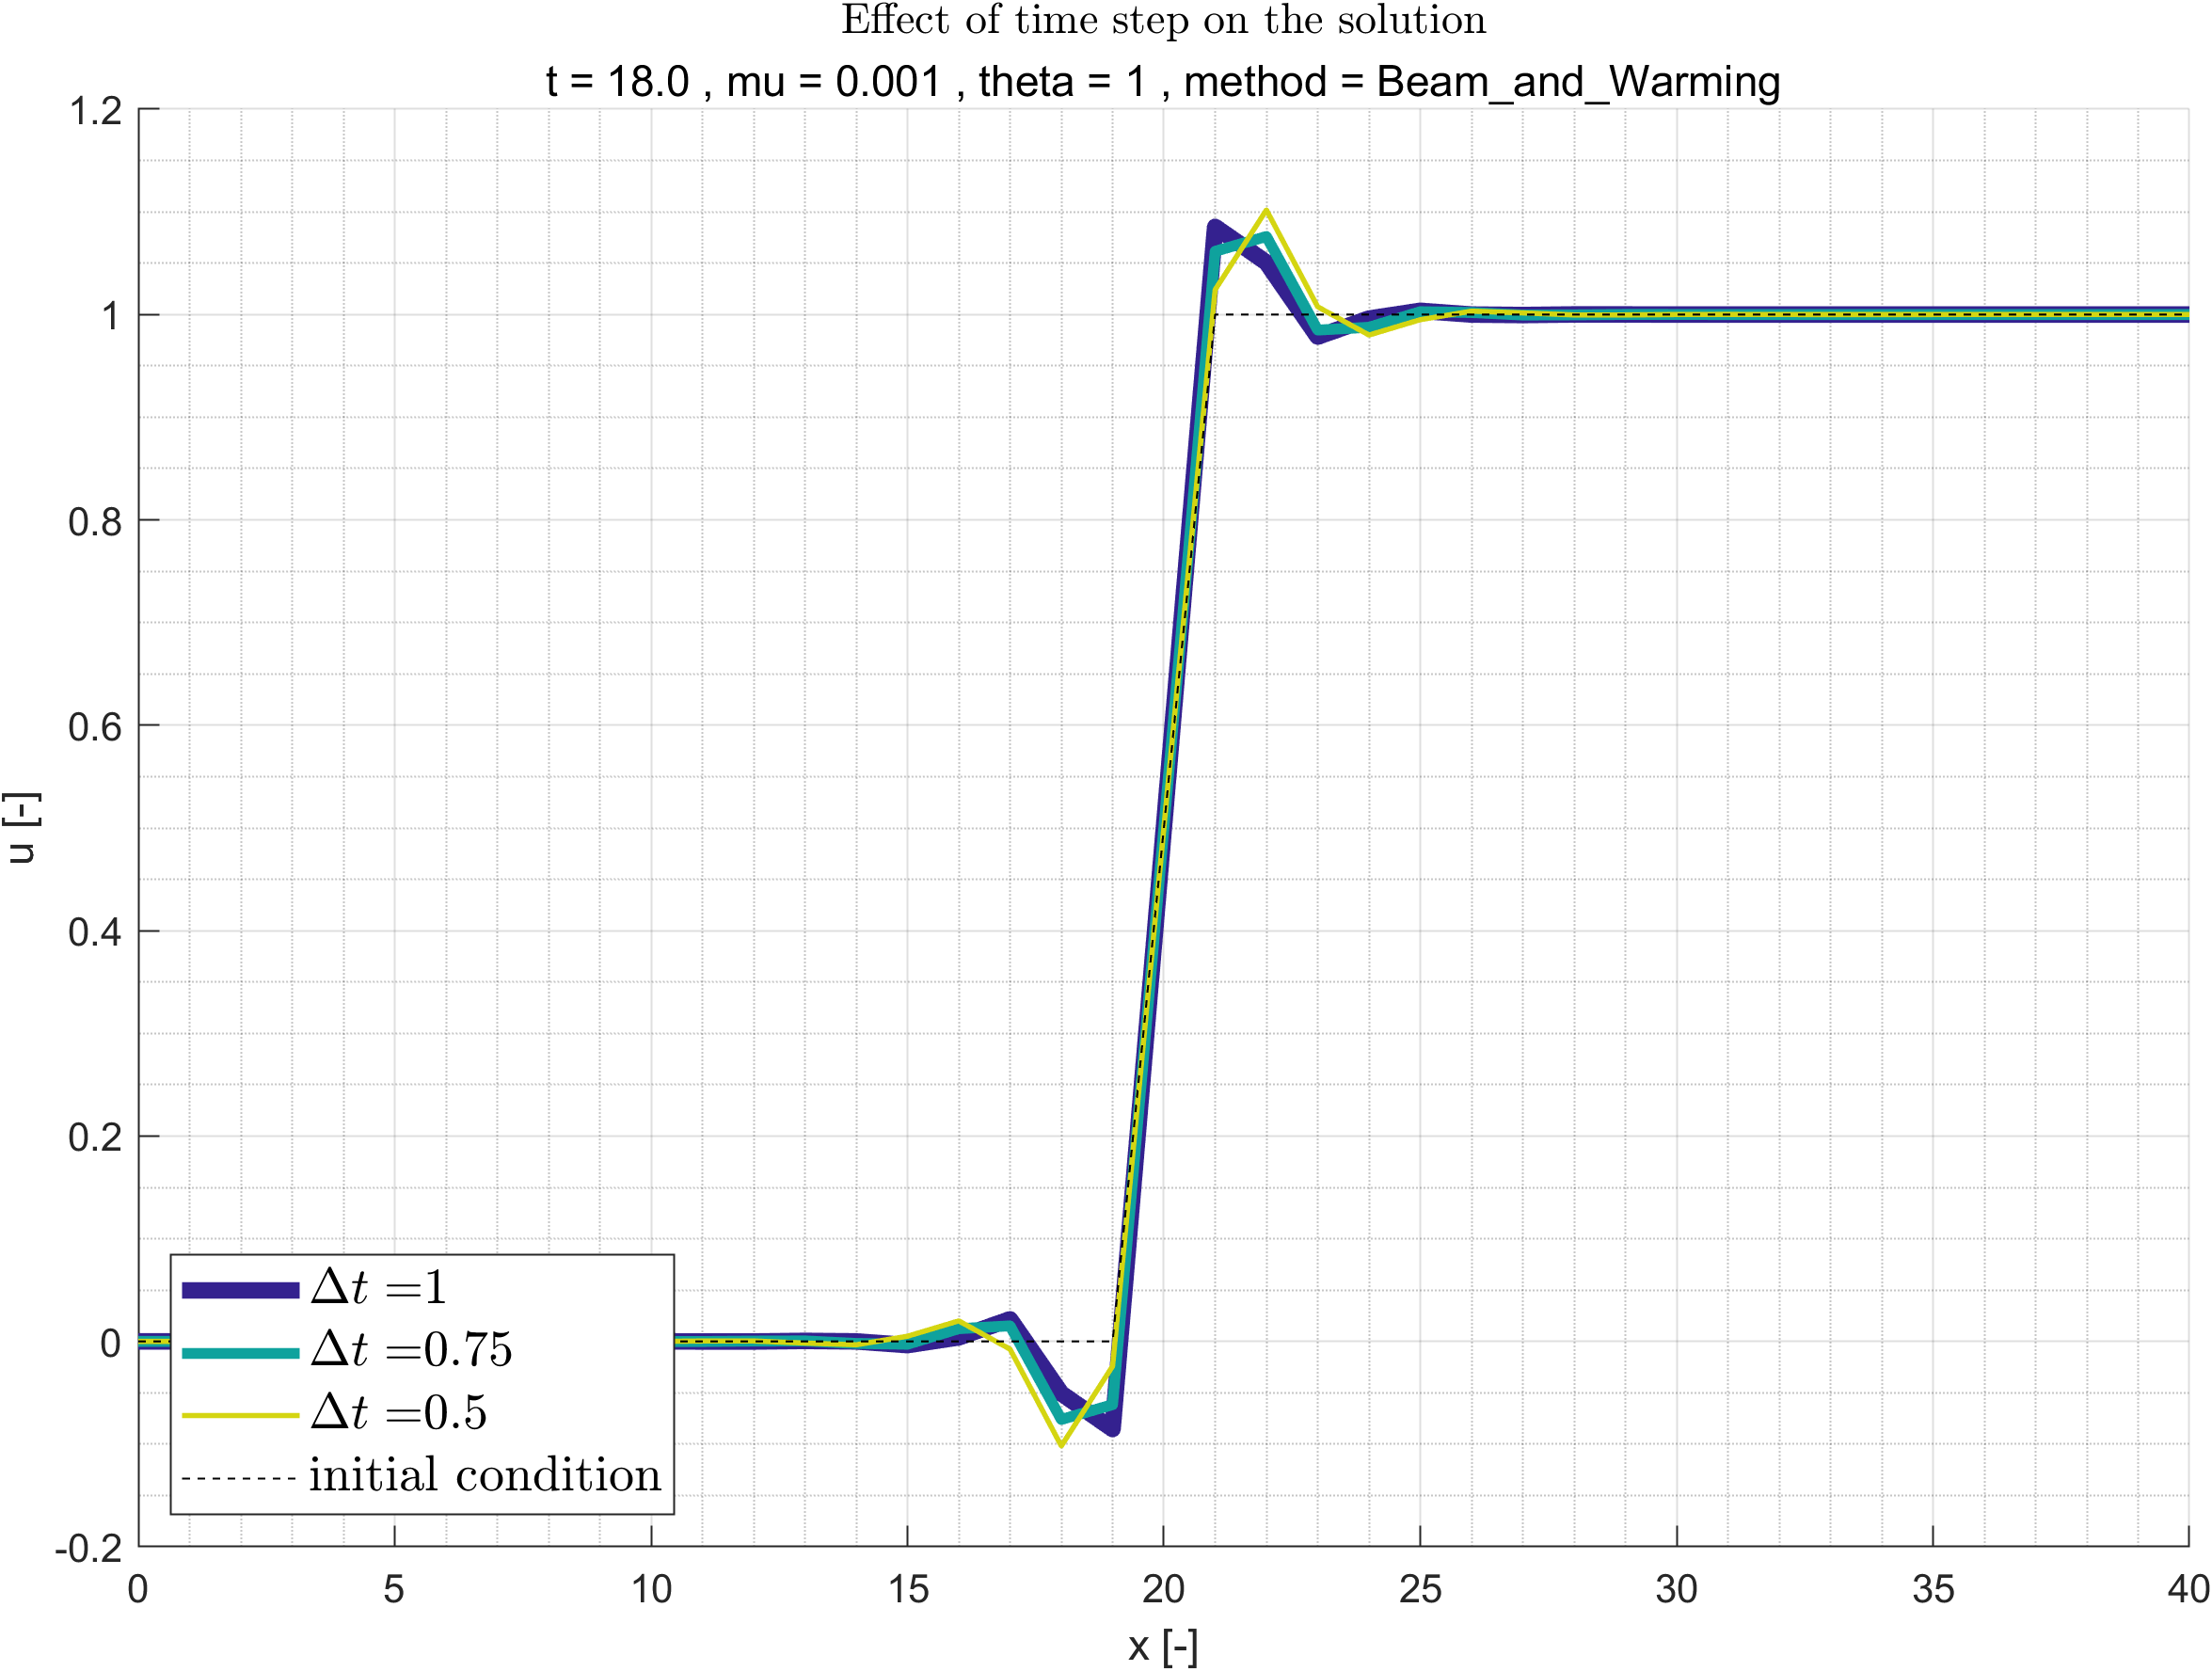
\includegraphics[width=\textwidth]{images/grap13.png}
        \caption{Beam $\&$ Warming $\mu=0.001,\ \theta=1$}
        \label{fig:Beam & Warming_general_mu0.001_theta1_A_diff_time}
    \end{subfigure}
    % \hfill
    \begin{subfigure}[c]{.38\textwidth}
        \centering
        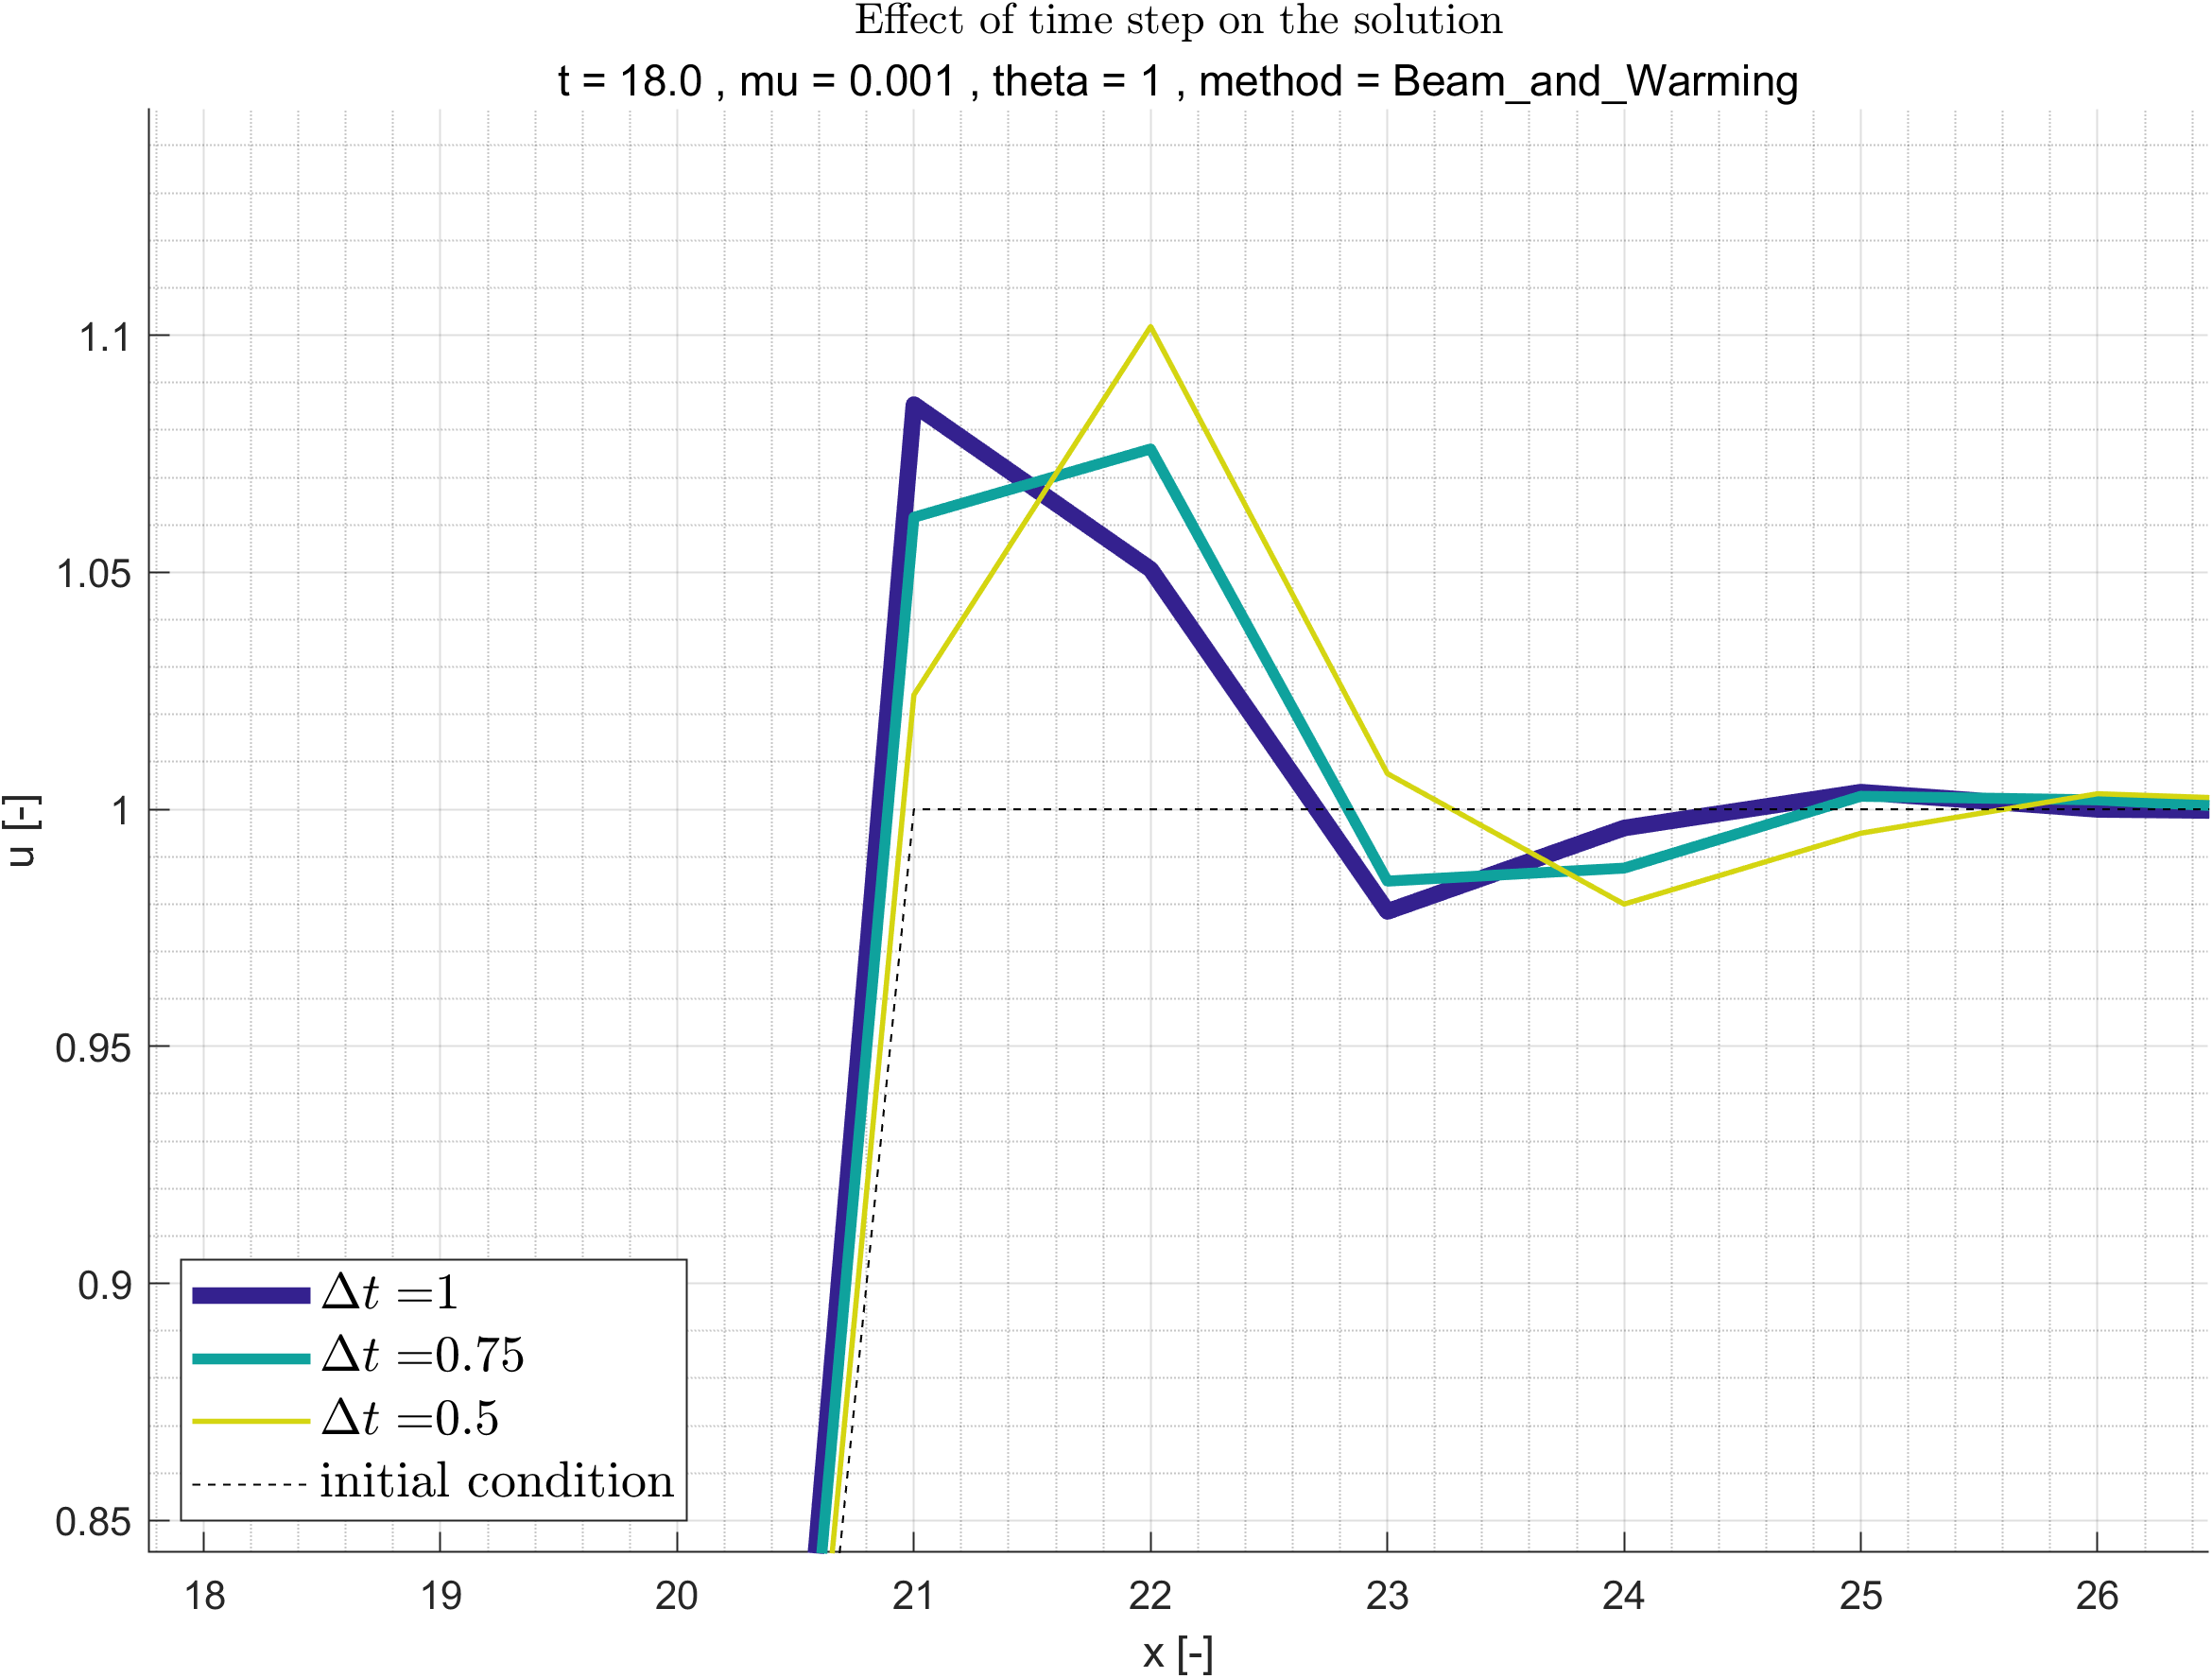
\includegraphics[width=\textwidth]{images/grap13.1.png}
        \caption{Beam $\&$ Warming $\mu=0.001,\ \theta=1$ - zoomed}
        \label{fig:Beam_&_Warming_general_mu0.001_theta1_B_diff_time}
    \end{subfigure}
    \begin{subfigure}[c]{.38\textwidth}
        \centering
        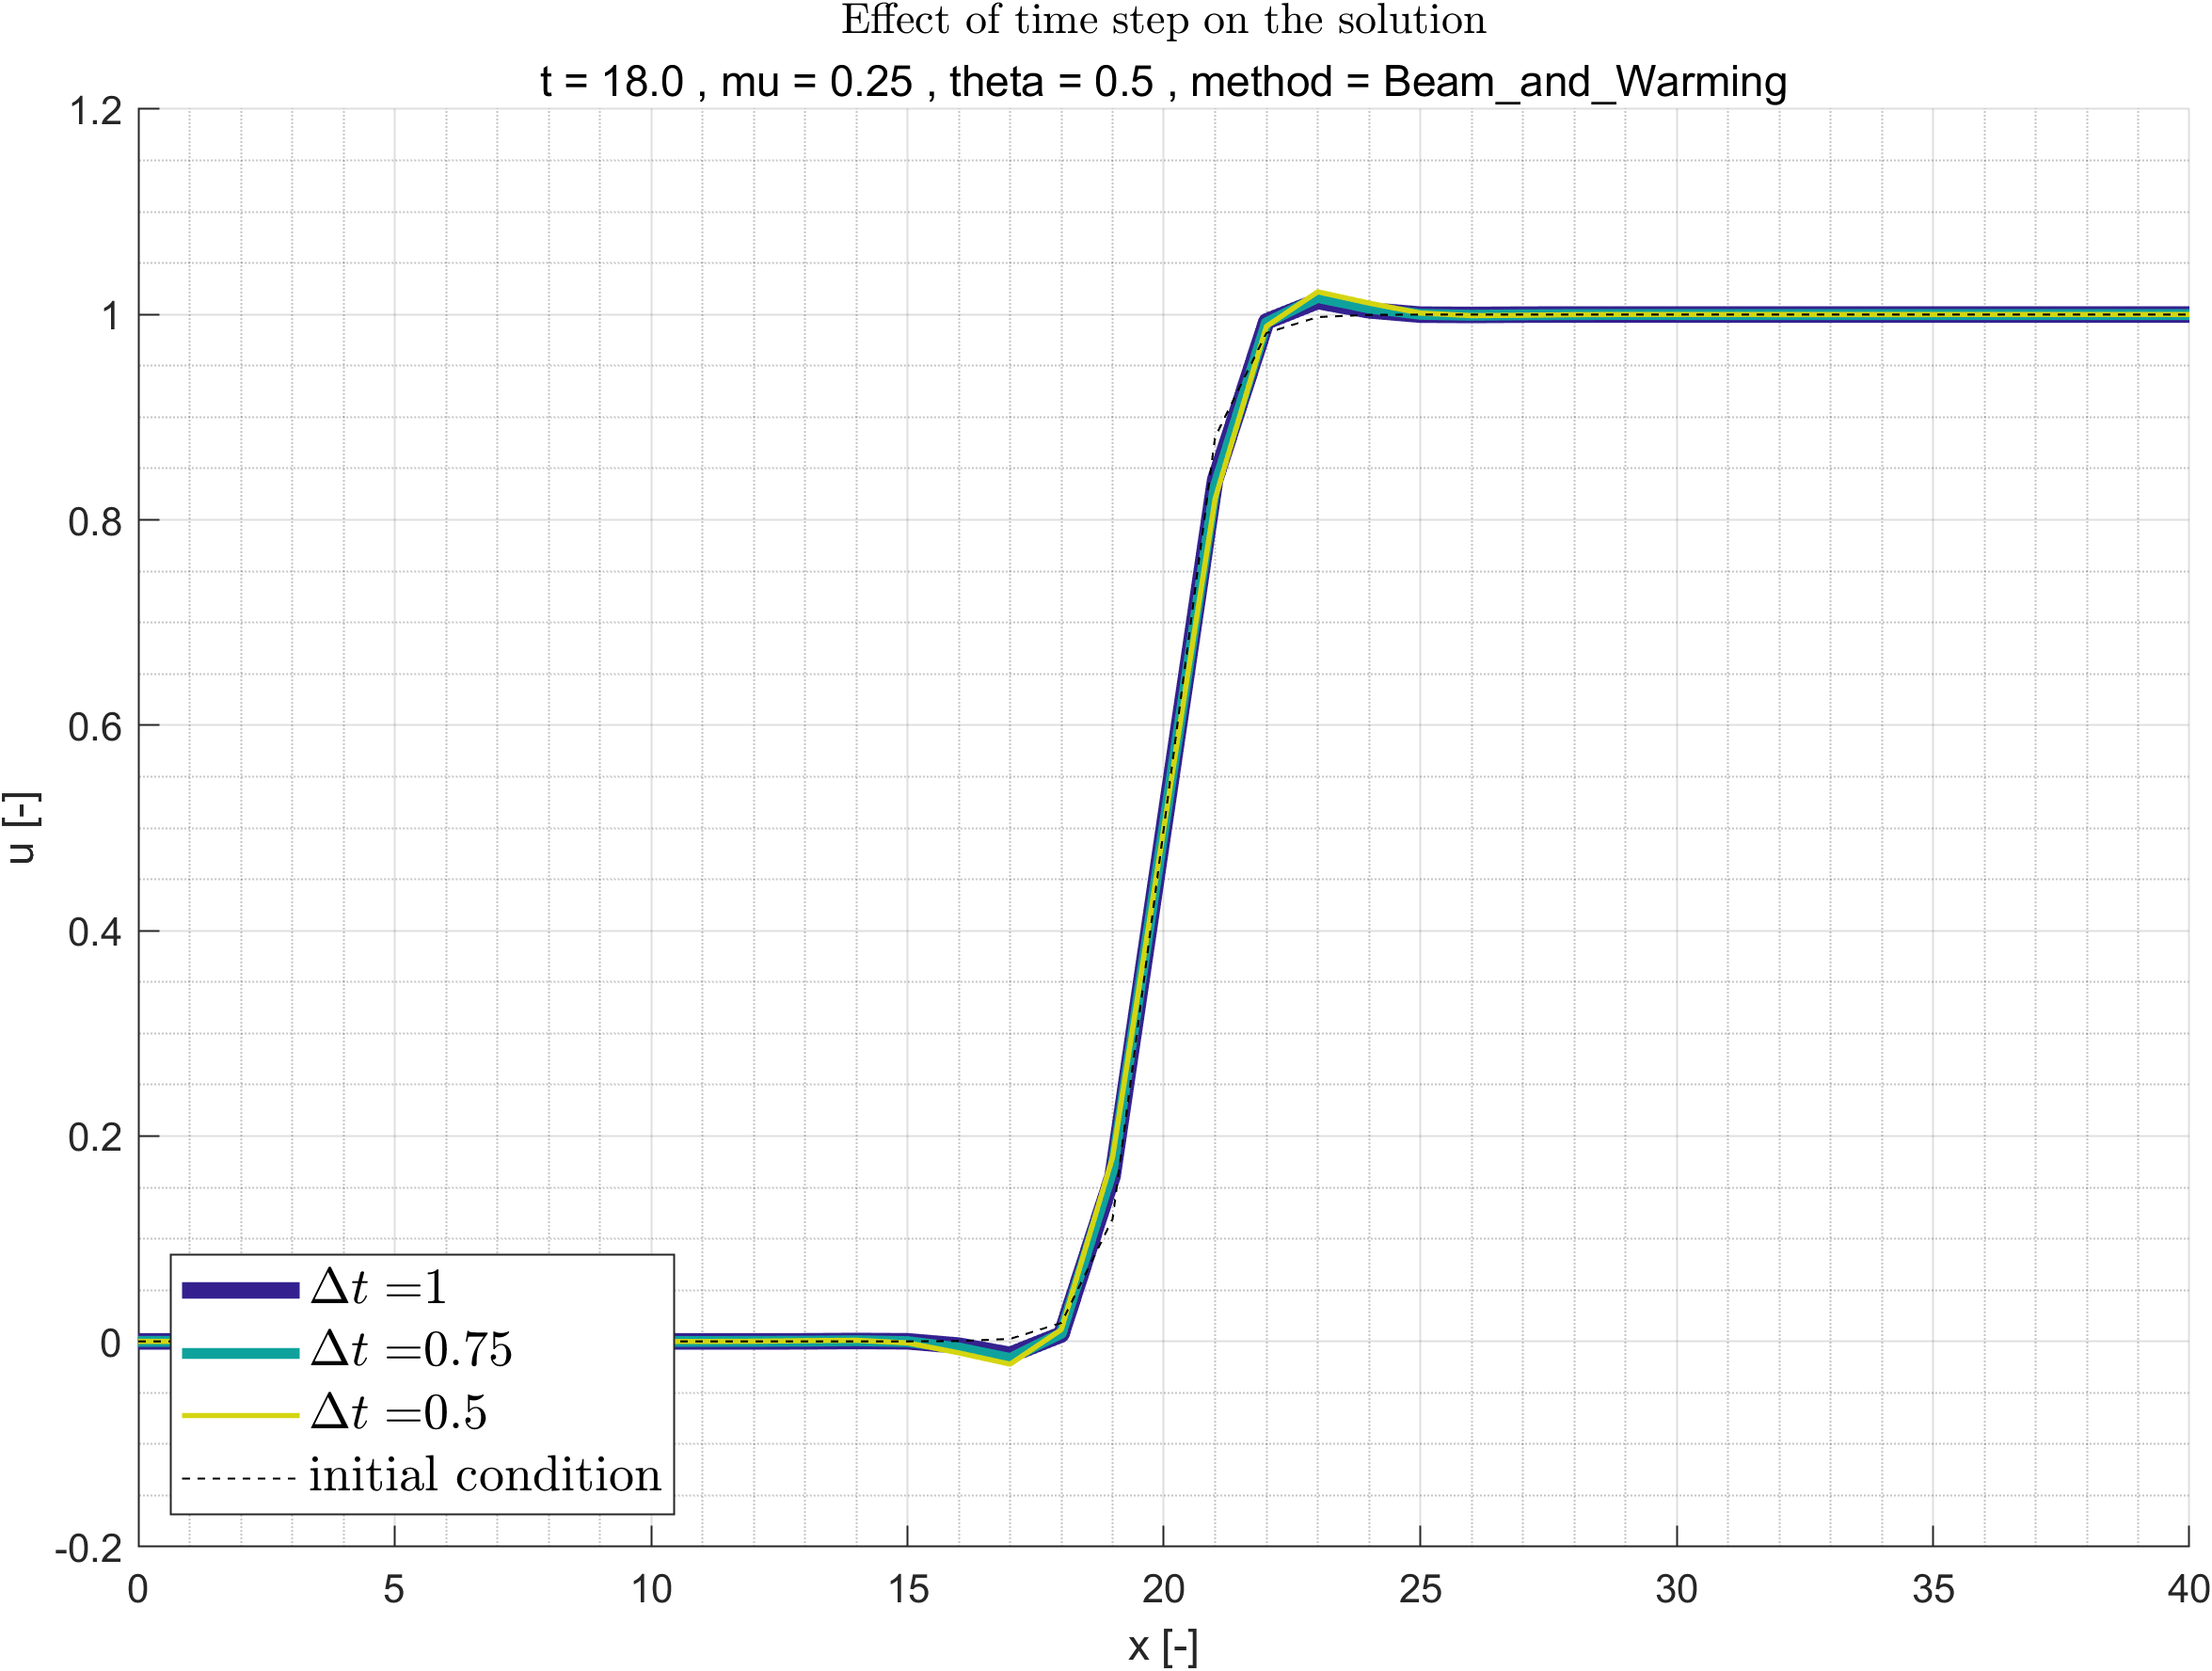
\includegraphics[width=\textwidth]{images/grap14.png}
        \caption{Beam $\&$ Warming $\mu=0.25,\ \theta=0.5$}
        \label{fig:Beam & Warming_general_mu0.25_theta0.5_A_diff_time}
    \end{subfigure}
    % \hfill
    \begin{subfigure}[c]{.38\textwidth}
        \centering
        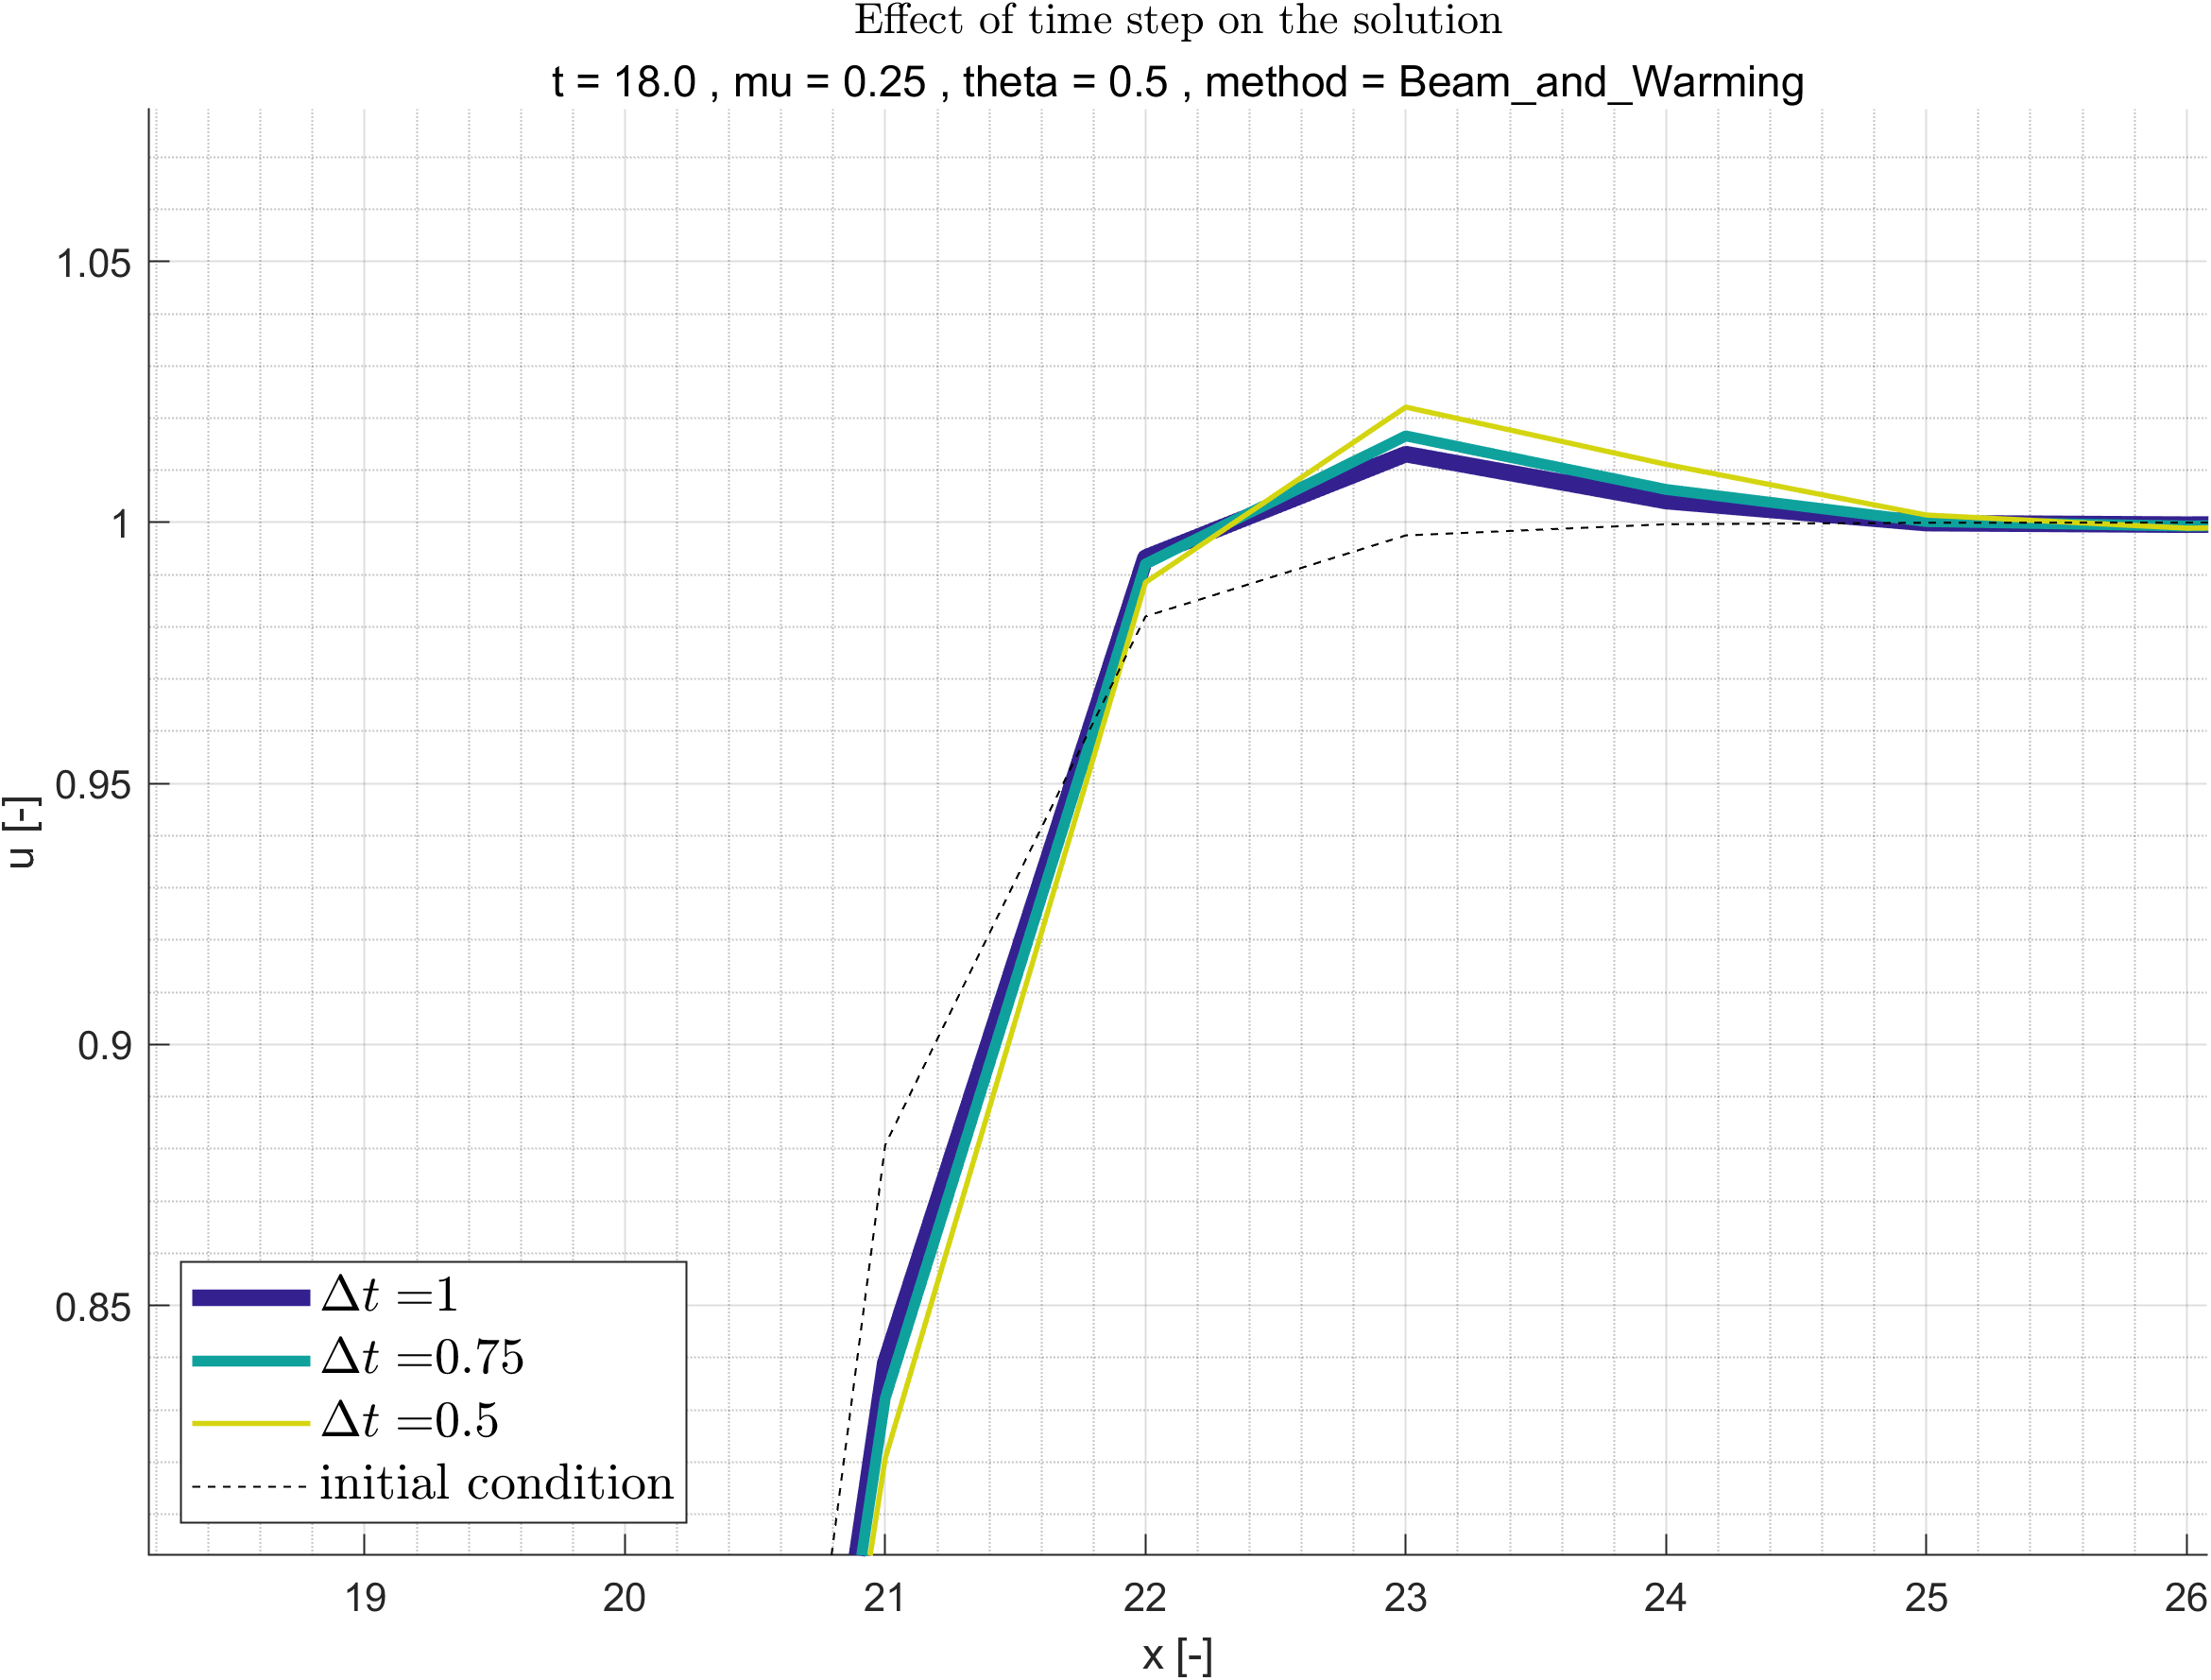
\includegraphics[width=\textwidth]{images/grap14.1.png}
        \caption{Beam $\&$ Warming $\mu=0.25,\ \theta=0.5$ - zoomed}
        \label{fig:Beam & Warming_general_mu0.25_theta0.5_B_diff_time}
    \end{subfigure}
    \begin{subfigure}[c]{.38\textwidth}
        \centering
        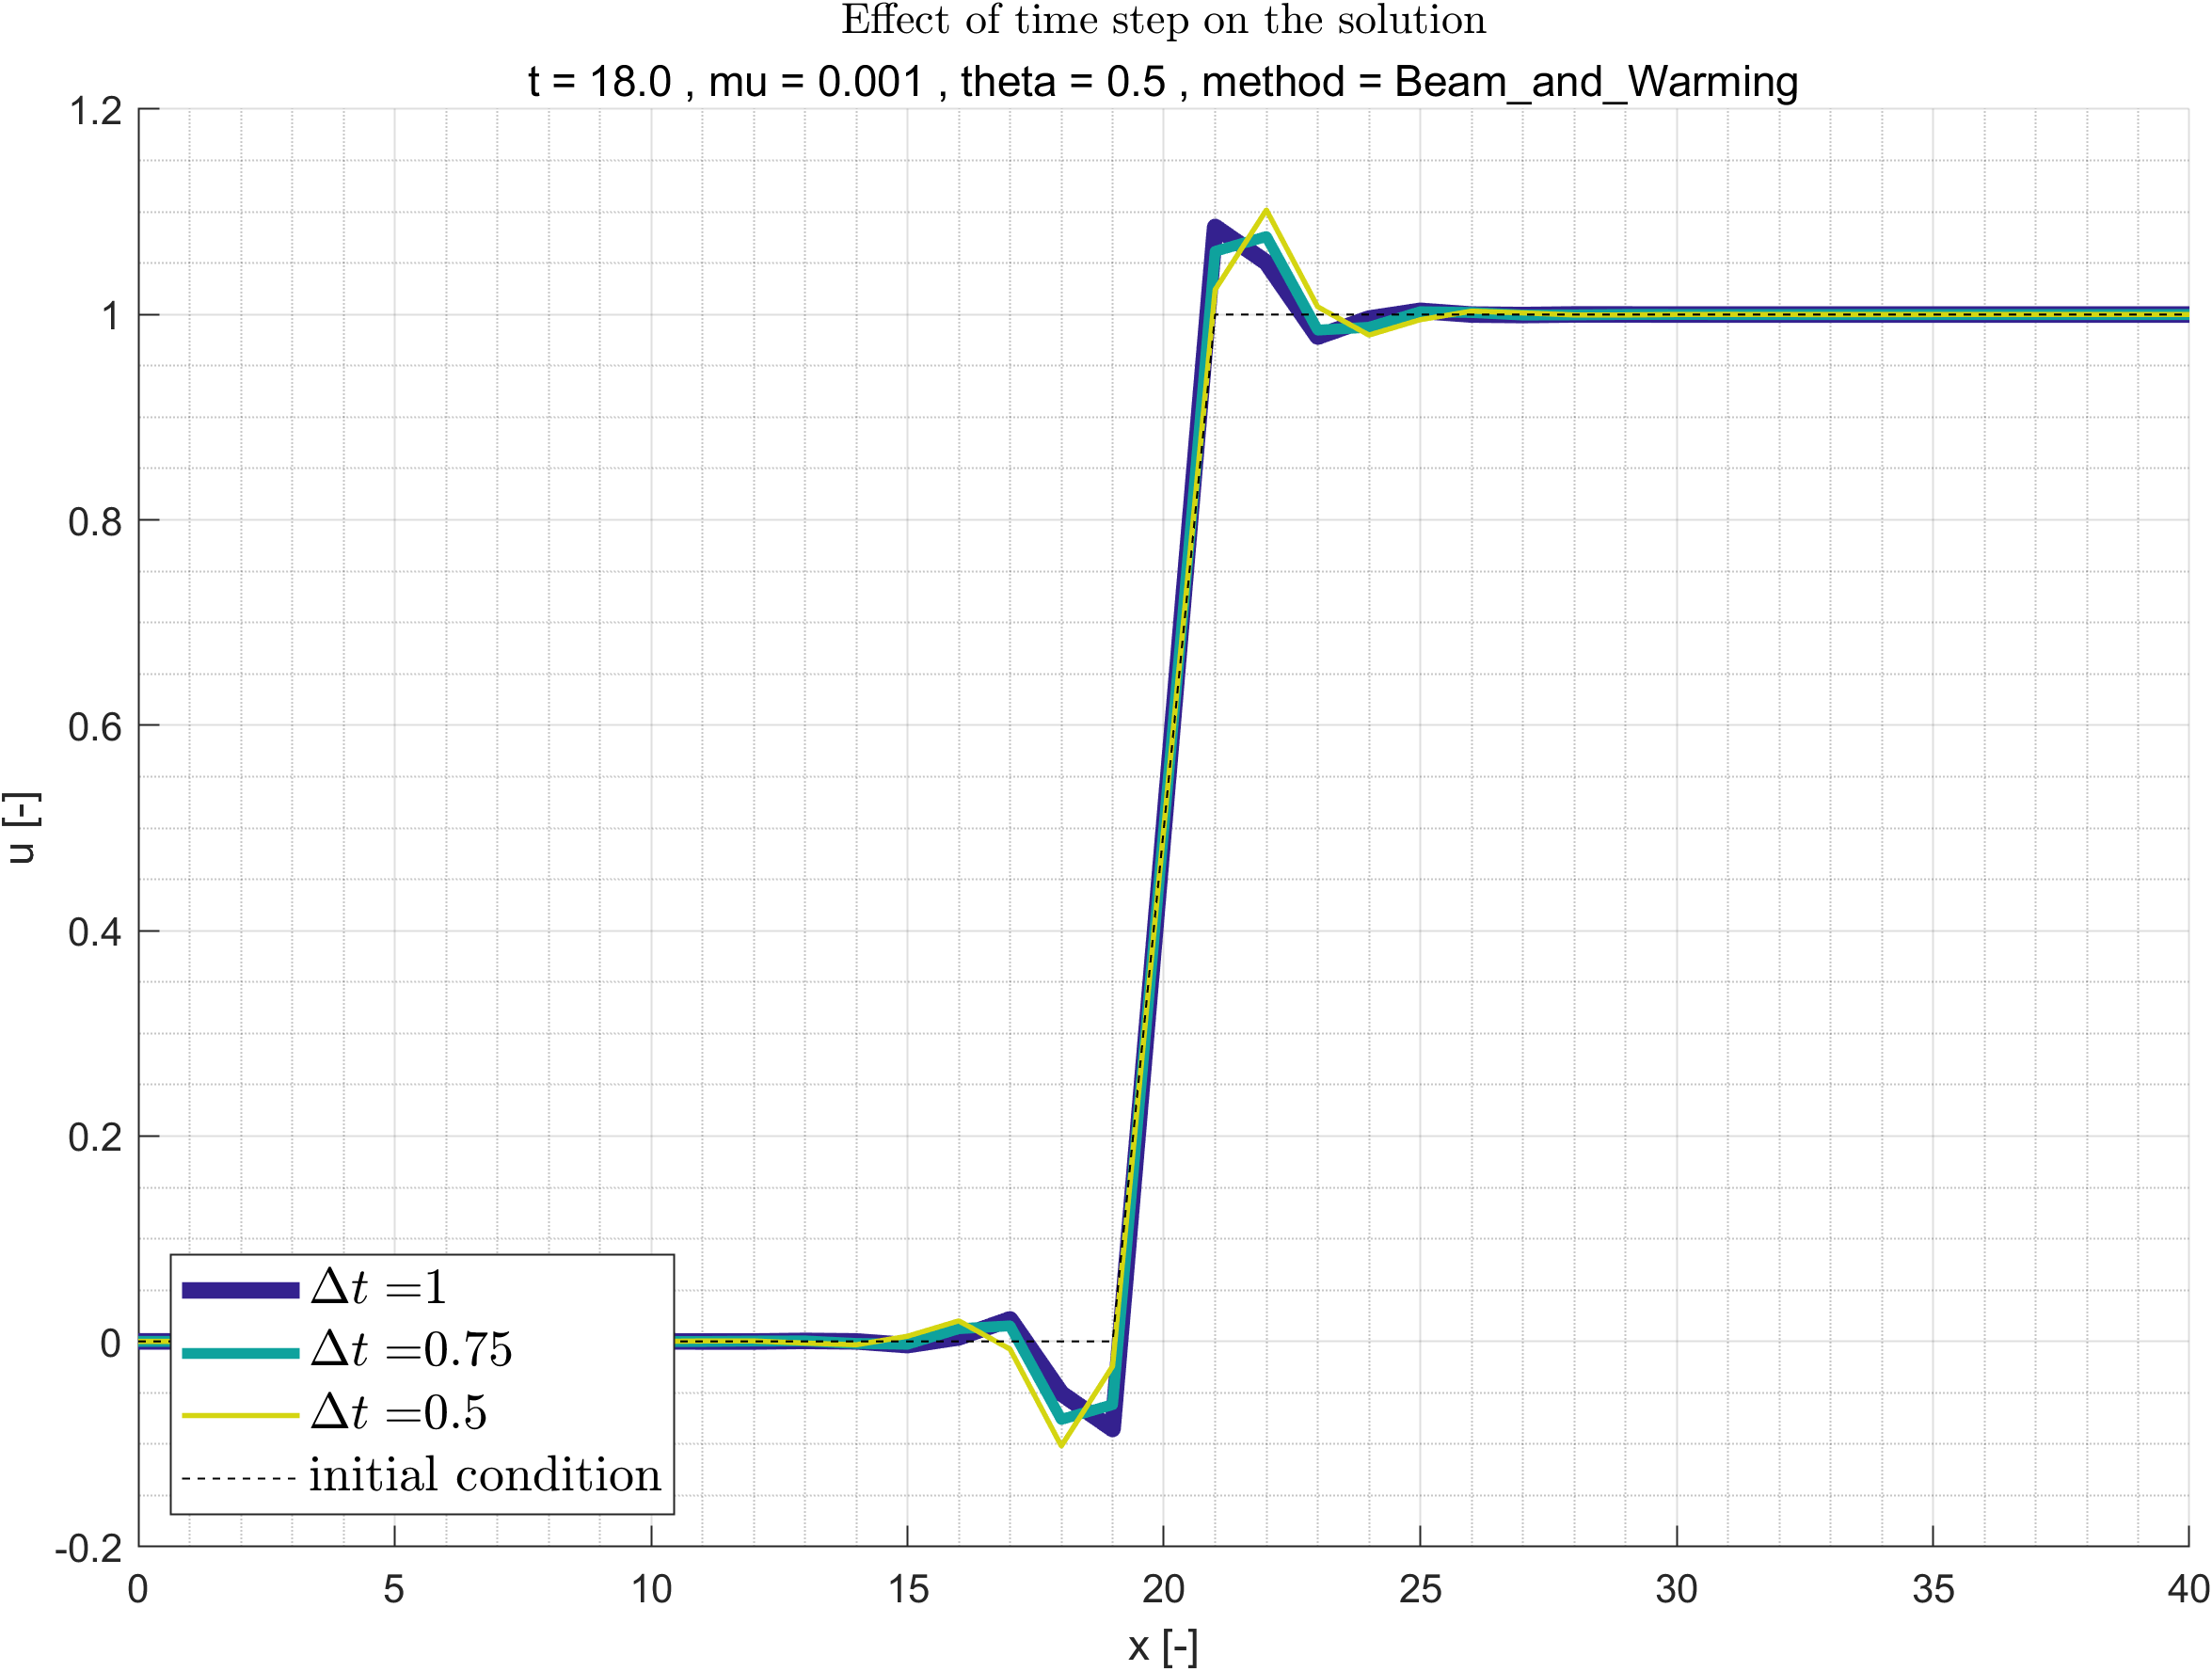
\includegraphics[width=\textwidth]{images/grap15.png}
        \caption{Beam $\&$ Warming $\mu=0.001,\ \theta=0.5$}
        \label{fig:Beam & Warming_general_mu0.001_theta0.5_A_diff_time}
    \end{subfigure}
    % \hfill
    \begin{subfigure}[c]{.38\textwidth}
        \centering
        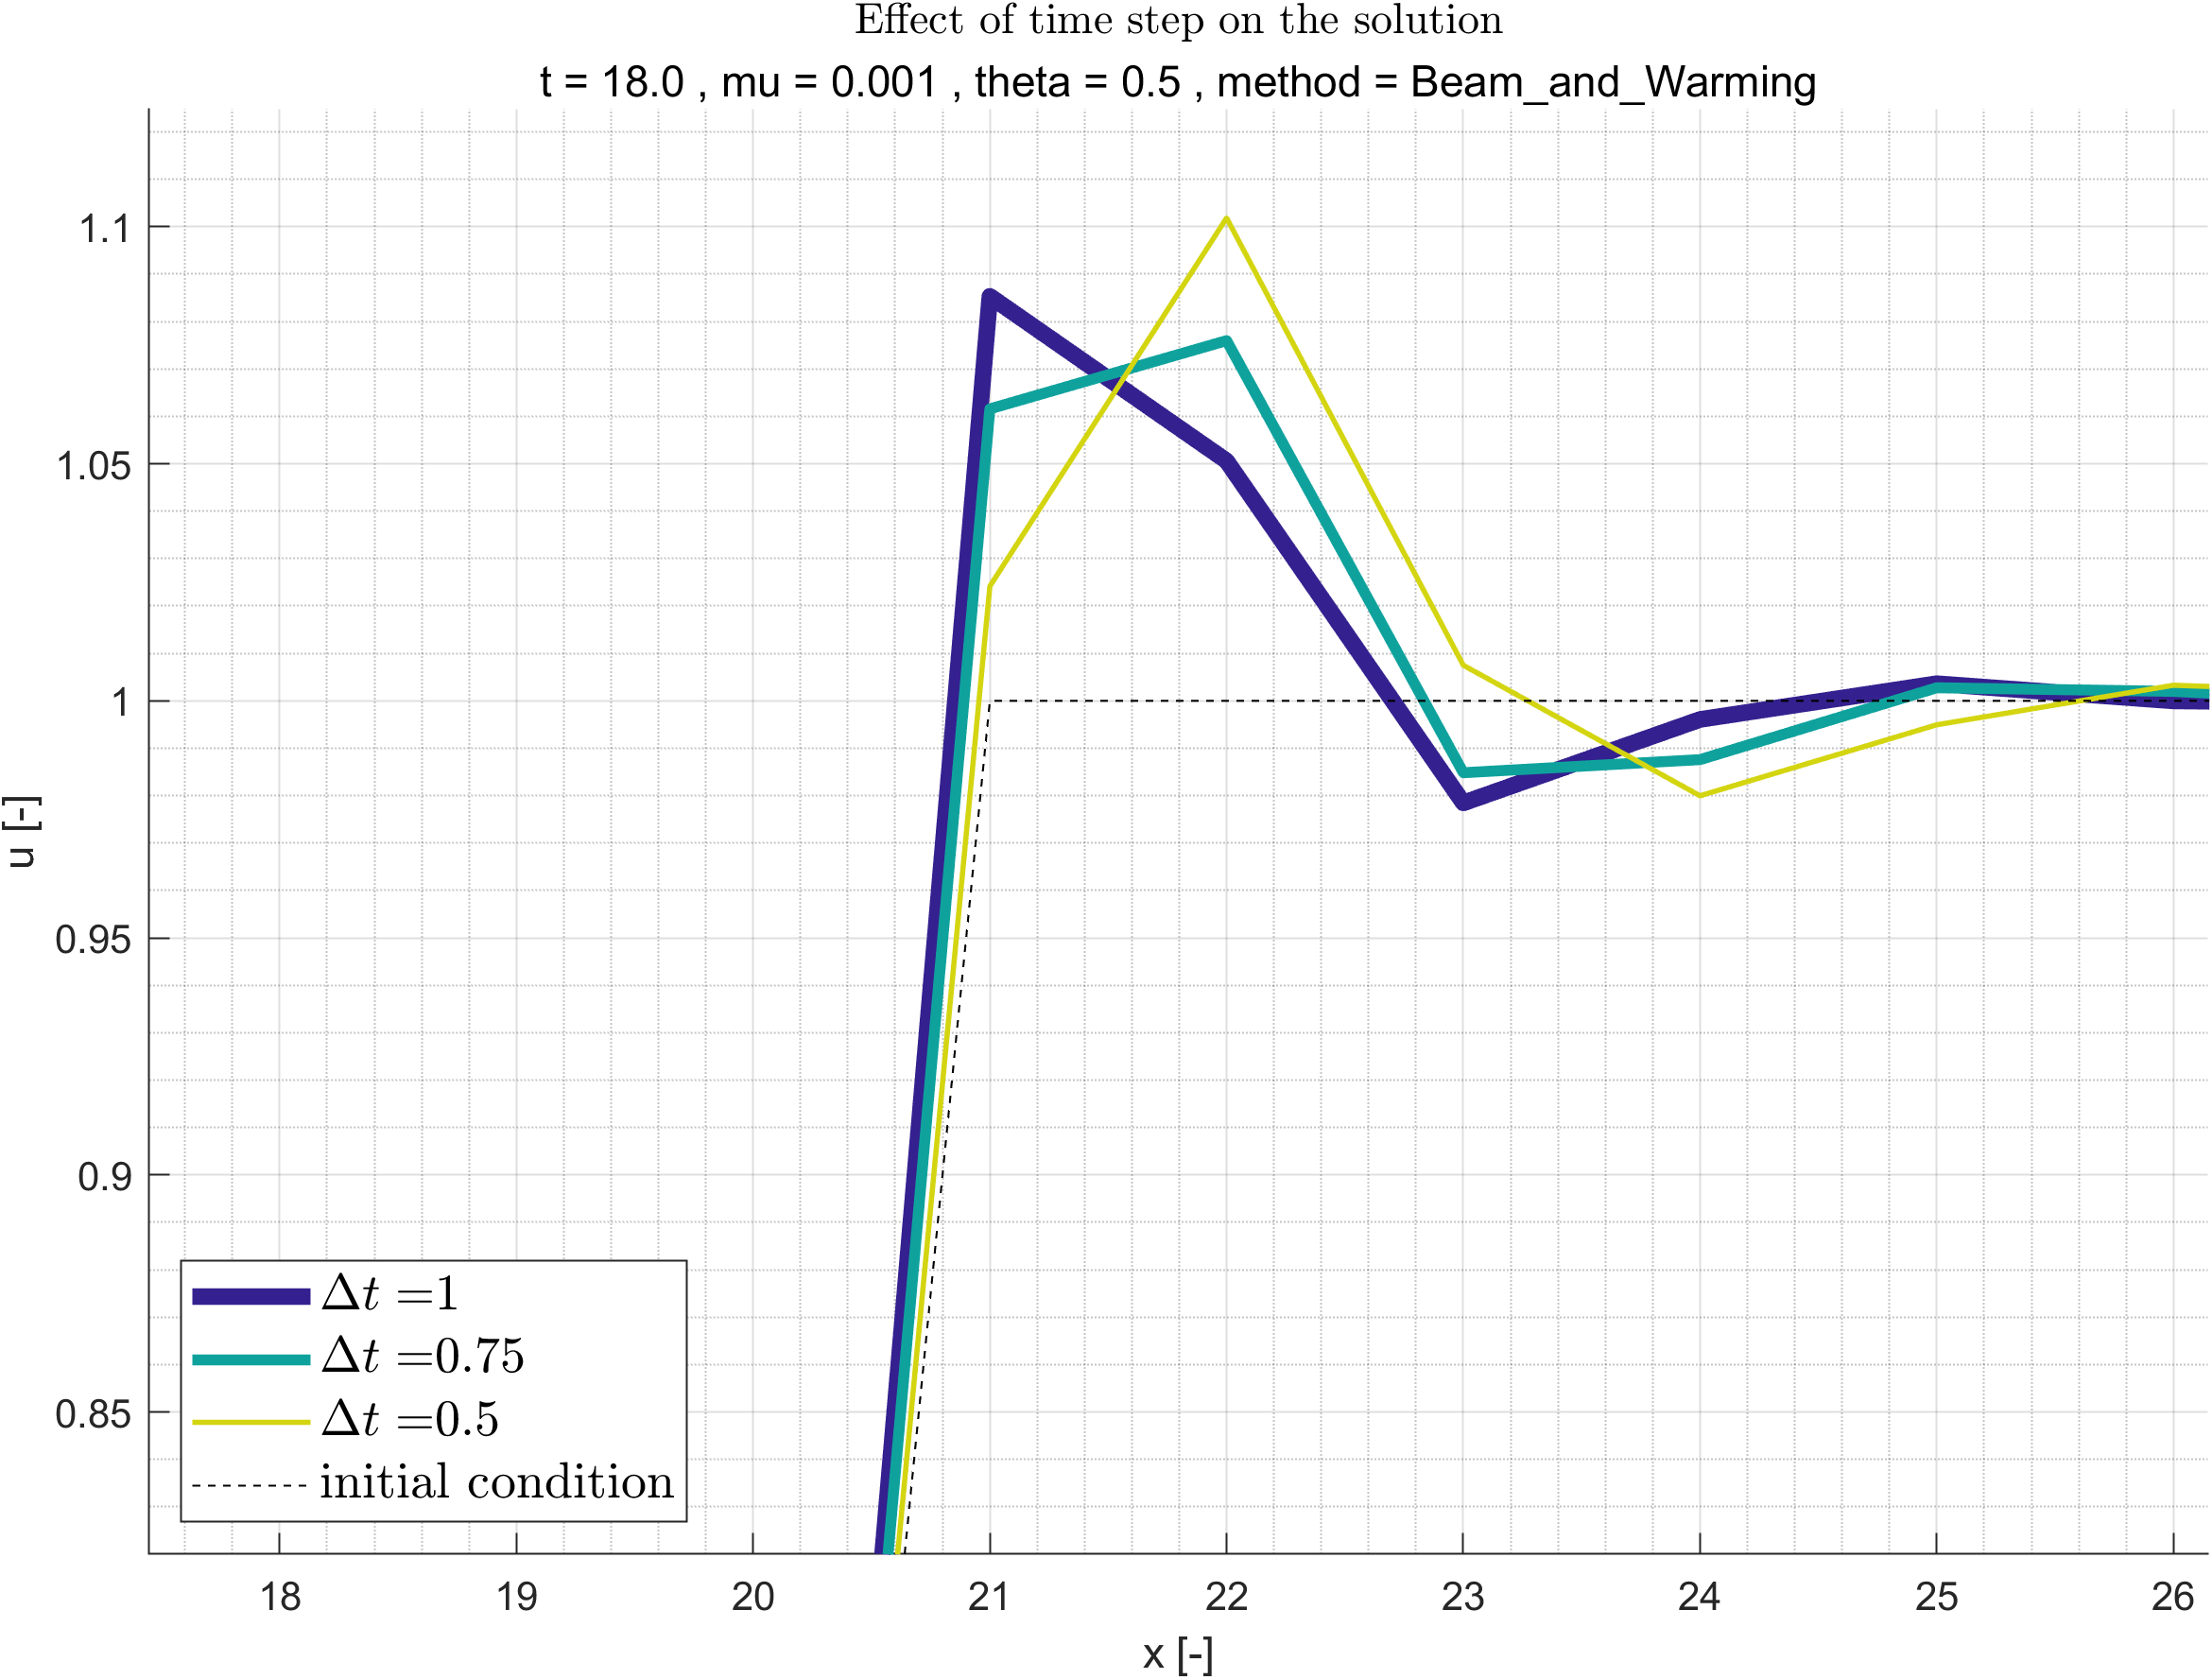
\includegraphics[width=\textwidth]{images/grap15.1.png}
        \caption{Beam $\&$ Warming $\mu=0.001,\ \theta=0.5$ - zoomed}
        \label{fig:Beam_&_Warming_general_mu0.001_theta0.5_B_diff_time}
    \end{subfigure}
    \caption{Effect of time step on solution - Beam $\&$ Warming}
        \label{fig:Beam_&_Warming_general_diff_time}
\end{figure}
We can see that when the viscosity is significant, the time step has near to no effect on the solution. When the viscosity is negligible, the time step has an effect on the solution, but unlike at the MacCormack method as the time step increases the oscillations does not decrease. It is visible that there is no visible difference between first order $\left(\theta=1\right)$ and second order $\left(\theta=0.5\right)$.

\subsubsection{Effect of Smoothing}
\begin{figure}[H]
    \centering
    \begin{subfigure}[c]{.38\textwidth}
        \centering
        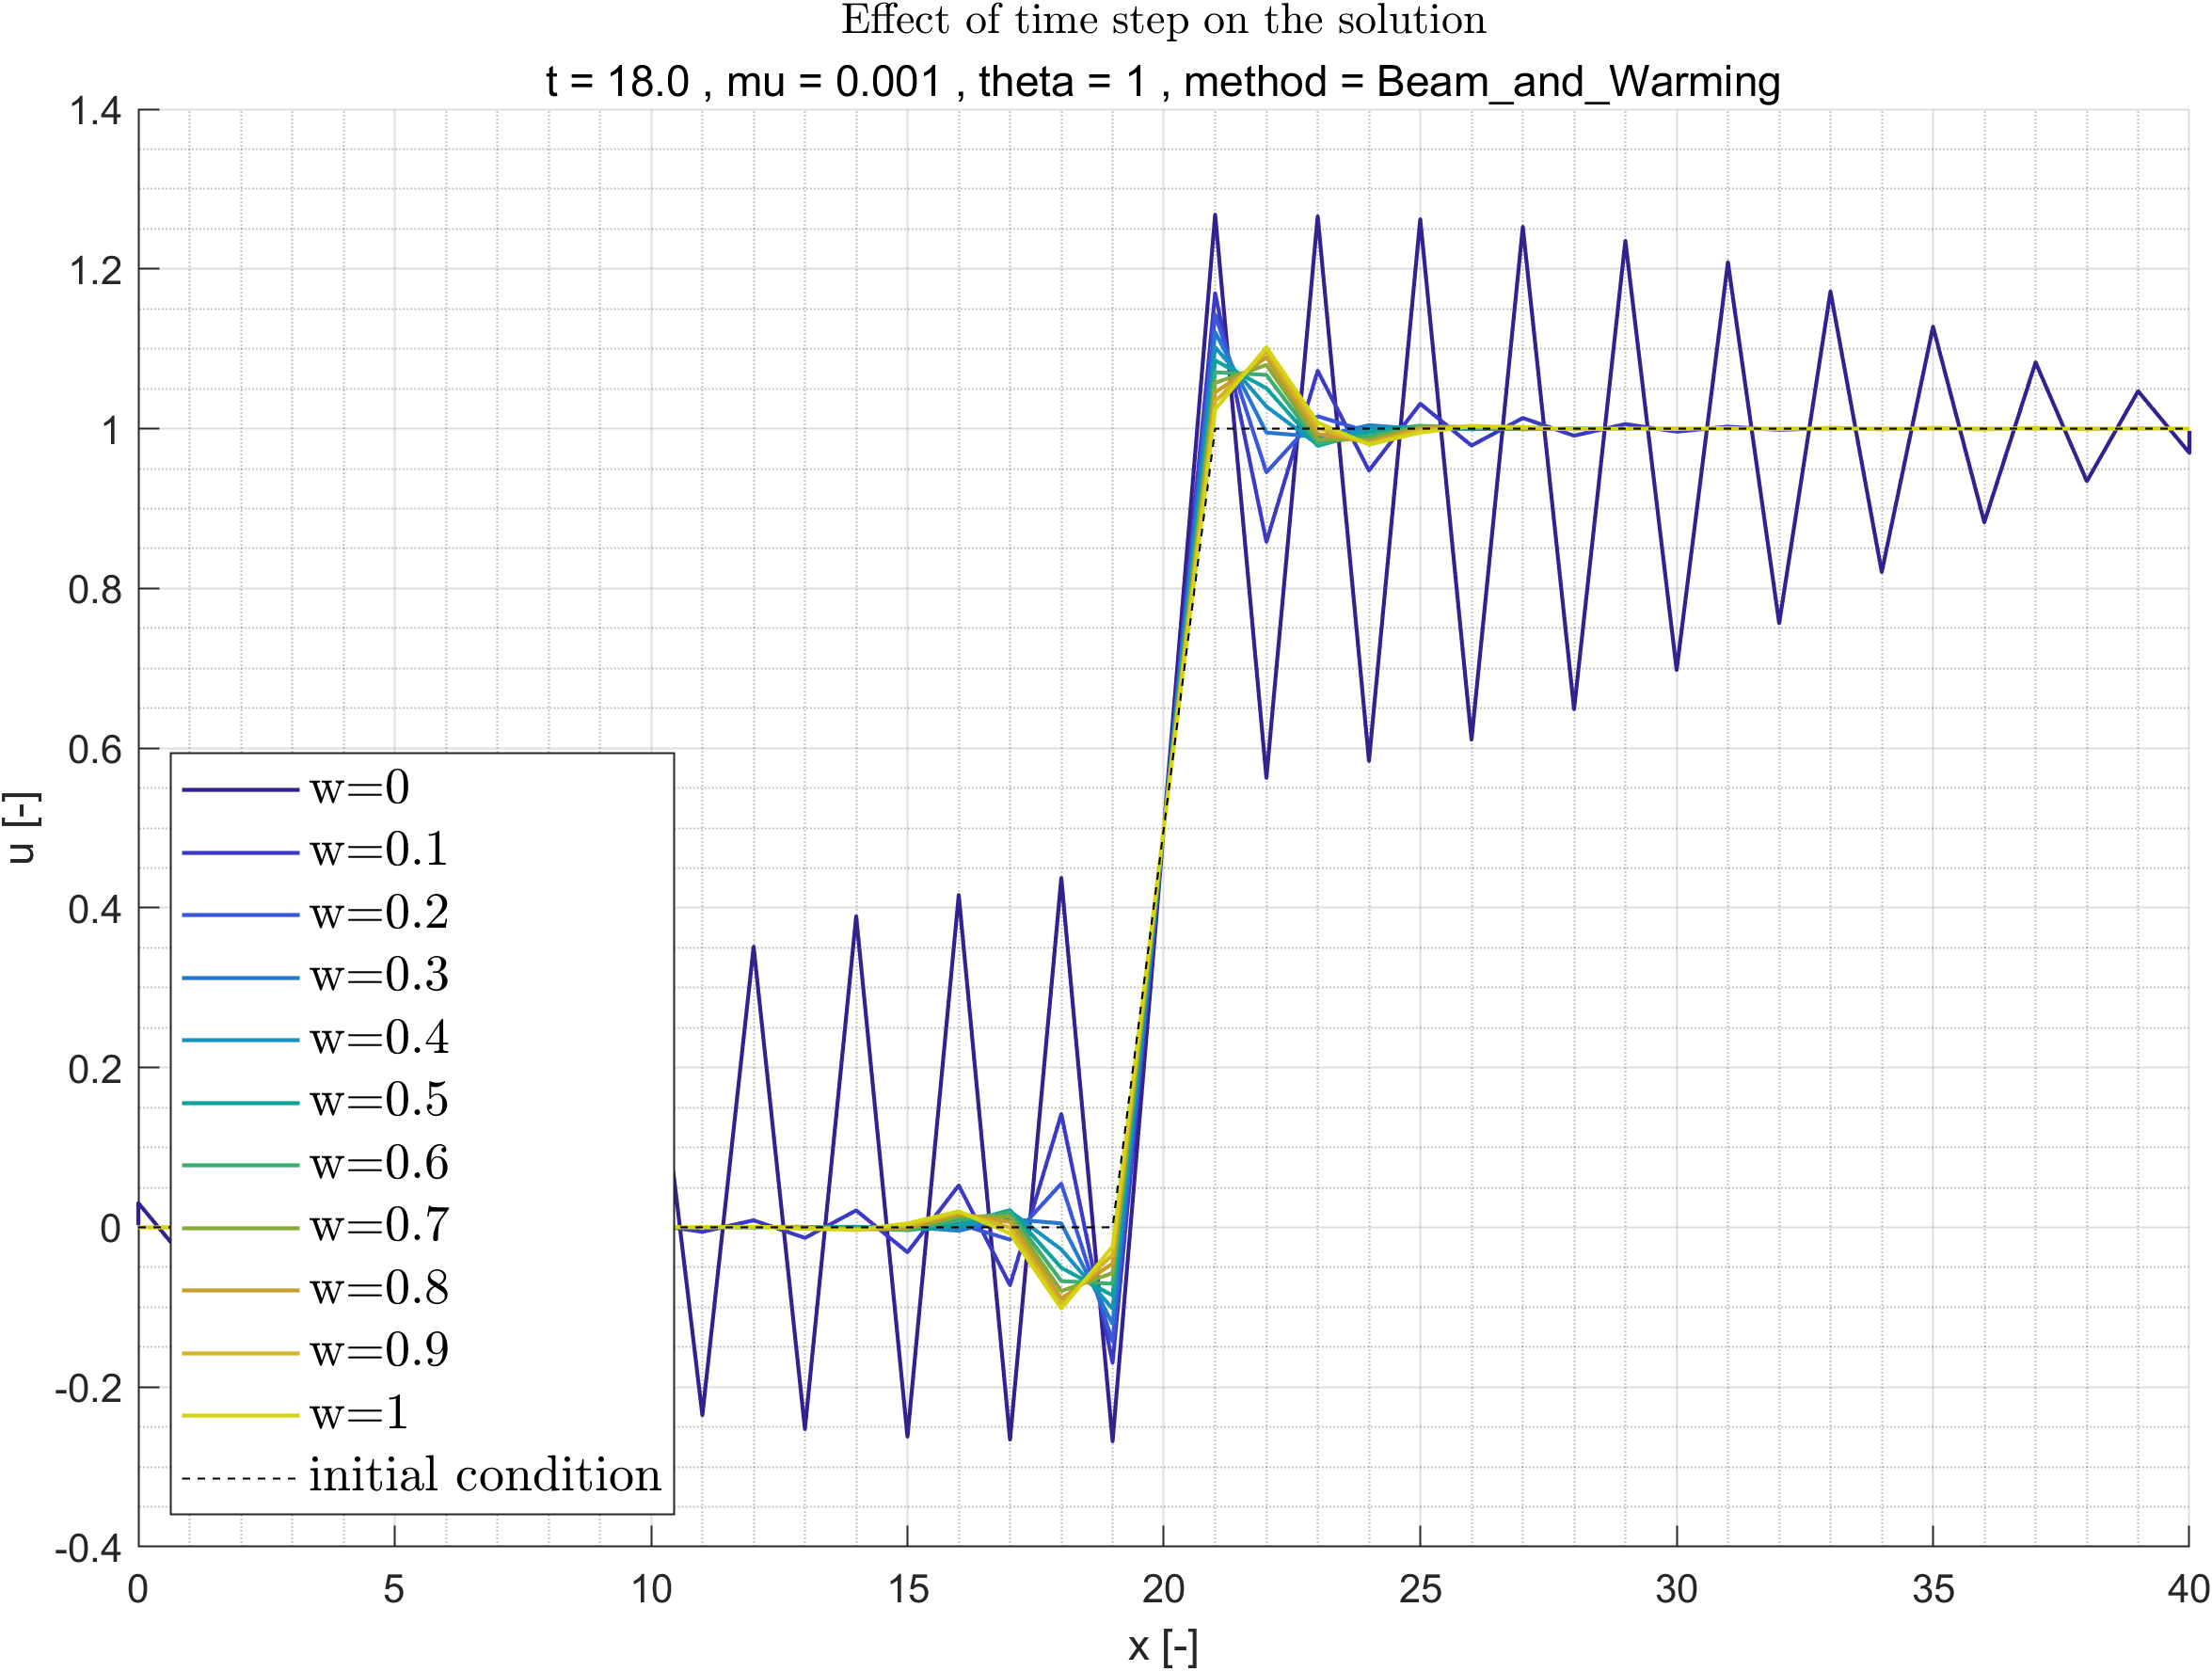
\includegraphics[width=\textwidth]{images/grap16.png}
        \caption{Beam $\&$ Warming $\mu=0.001,\ \theta=1$}
        \label{fig:Beam & Warming_general_mu0.001_theta1_A_diff_w}
    \end{subfigure}
    % \hfill
    \begin{subfigure}[c]{.38\textwidth}
        \centering
        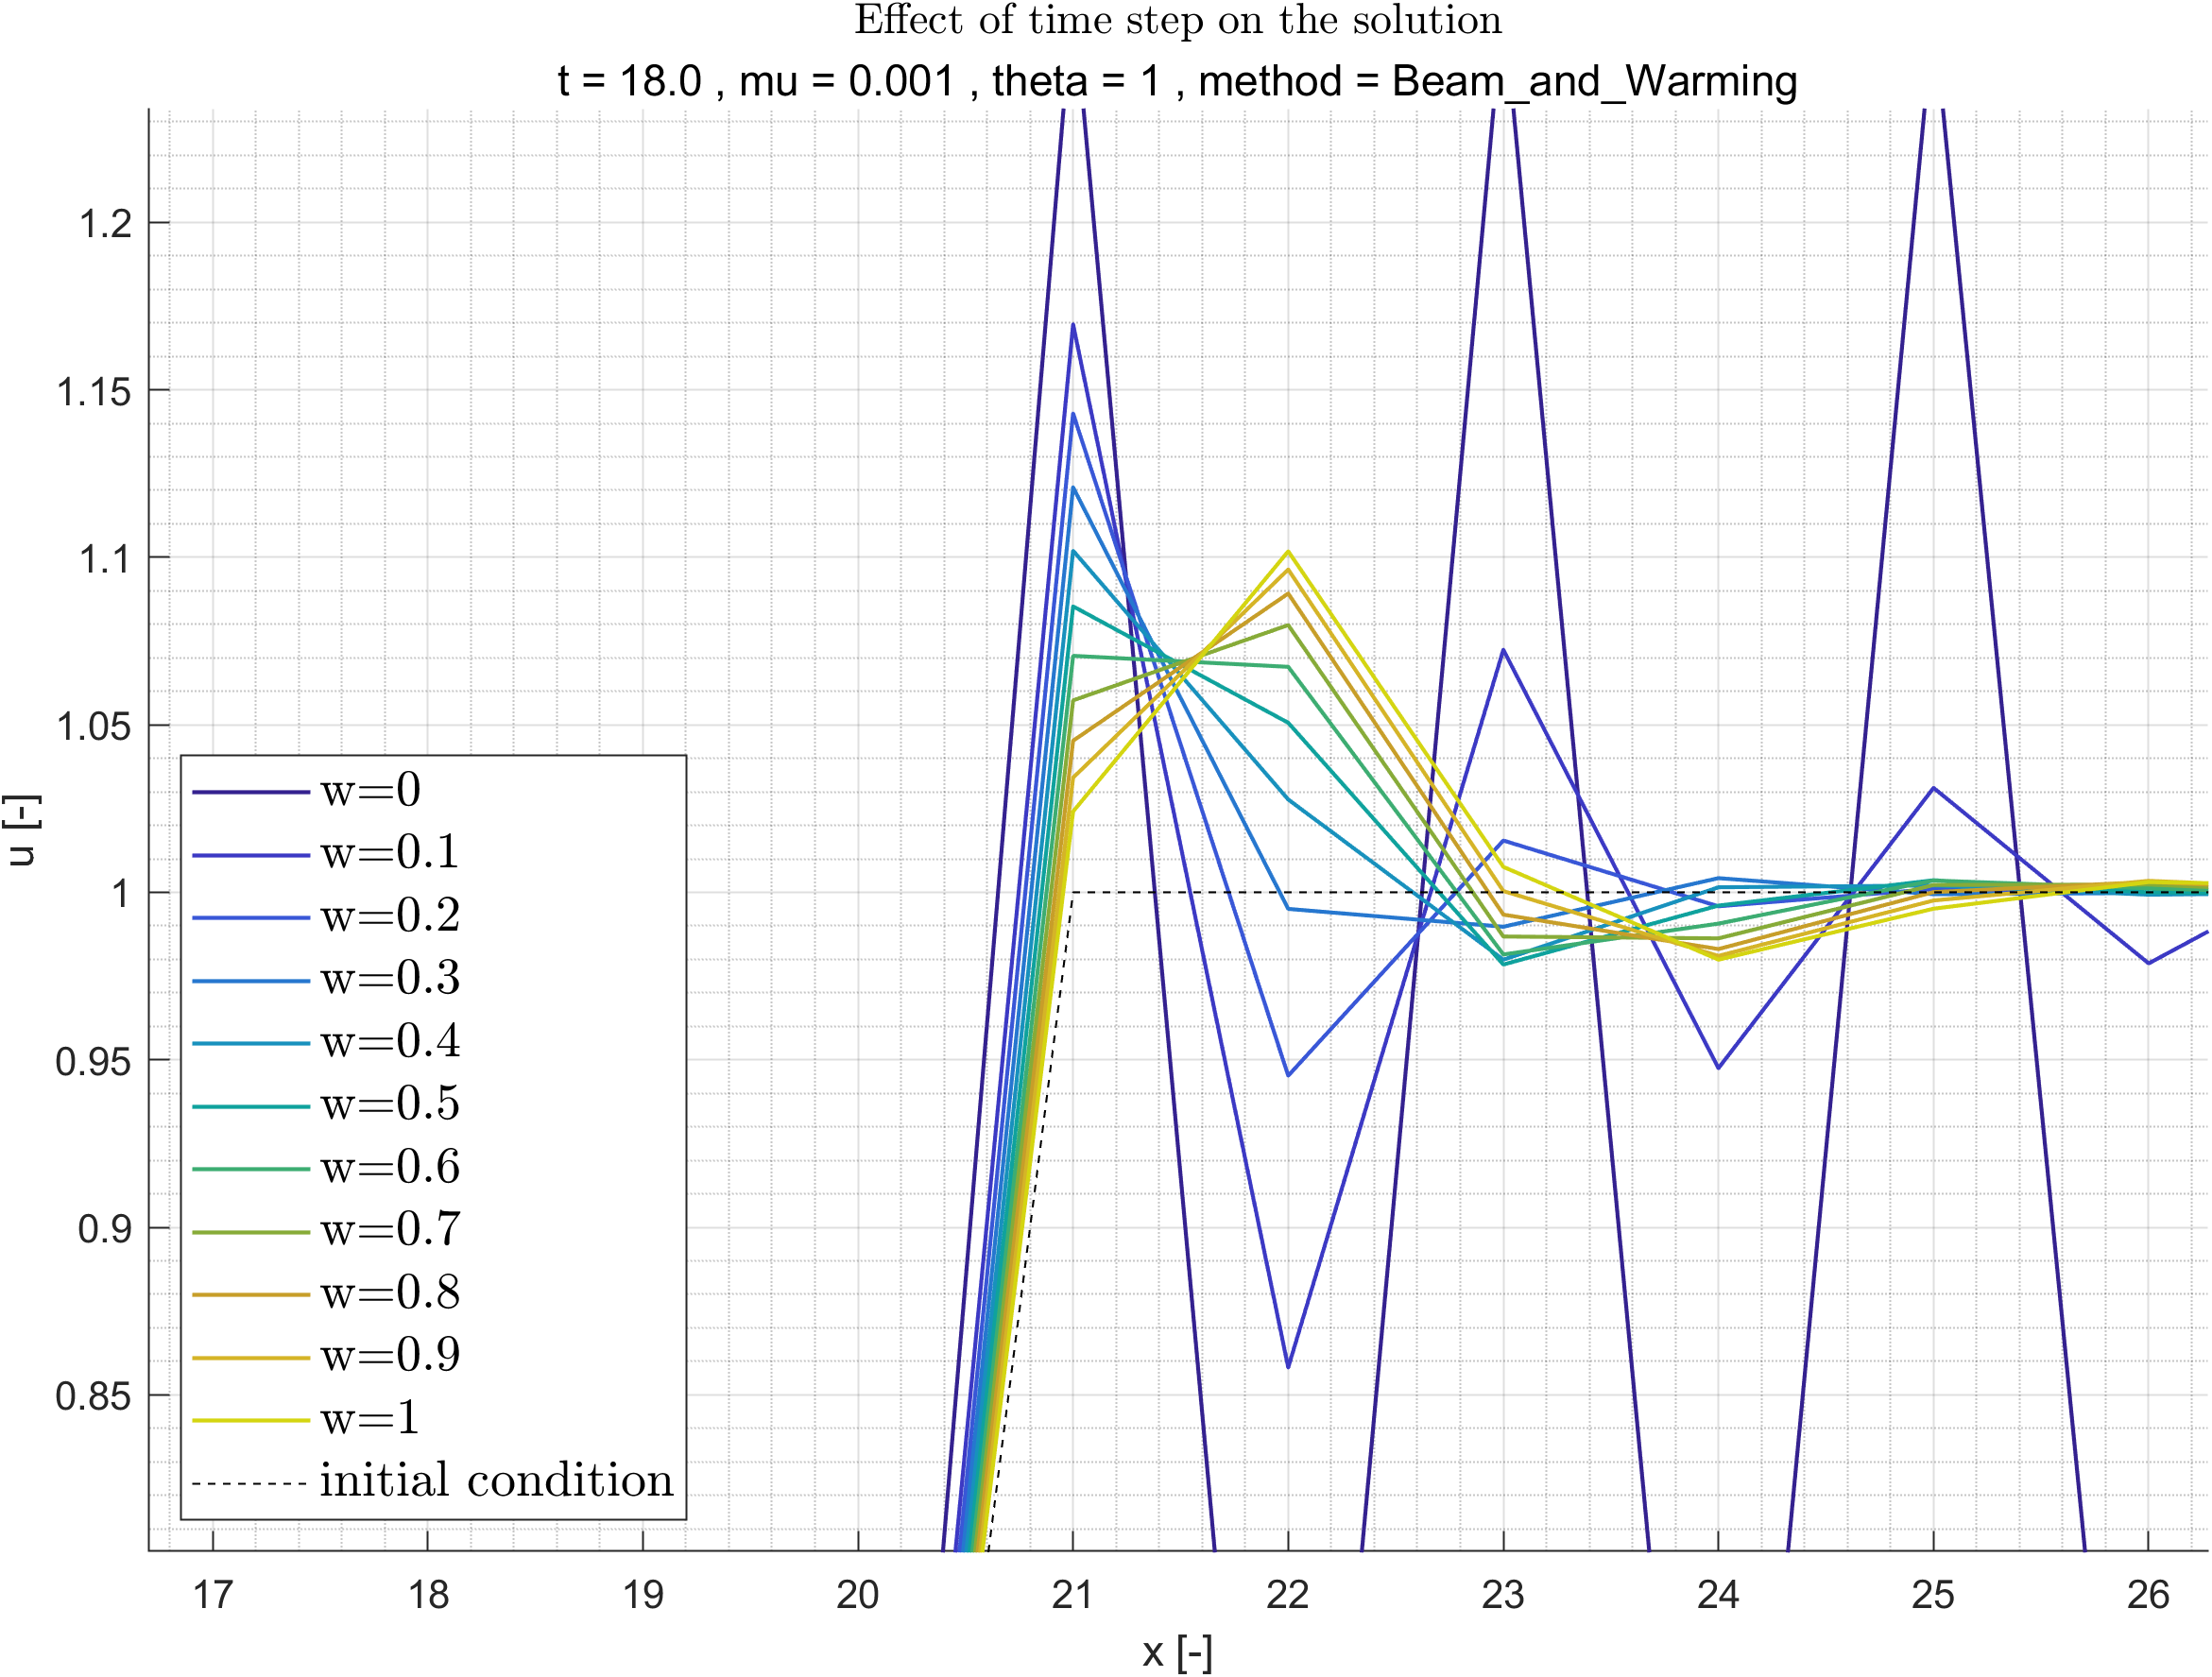
\includegraphics[width=\textwidth]{images/grap16.1.png}
        \caption{Beam $\&$ Warming $\mu=0.001,\ \theta=1$ - zoomed}
        \label{fig:Beam & Warming_general_mu0.001_theta1_B_diff_w}
    \end{subfigure}
    \begin{subfigure}[c]{.38\textwidth}
        \centering
        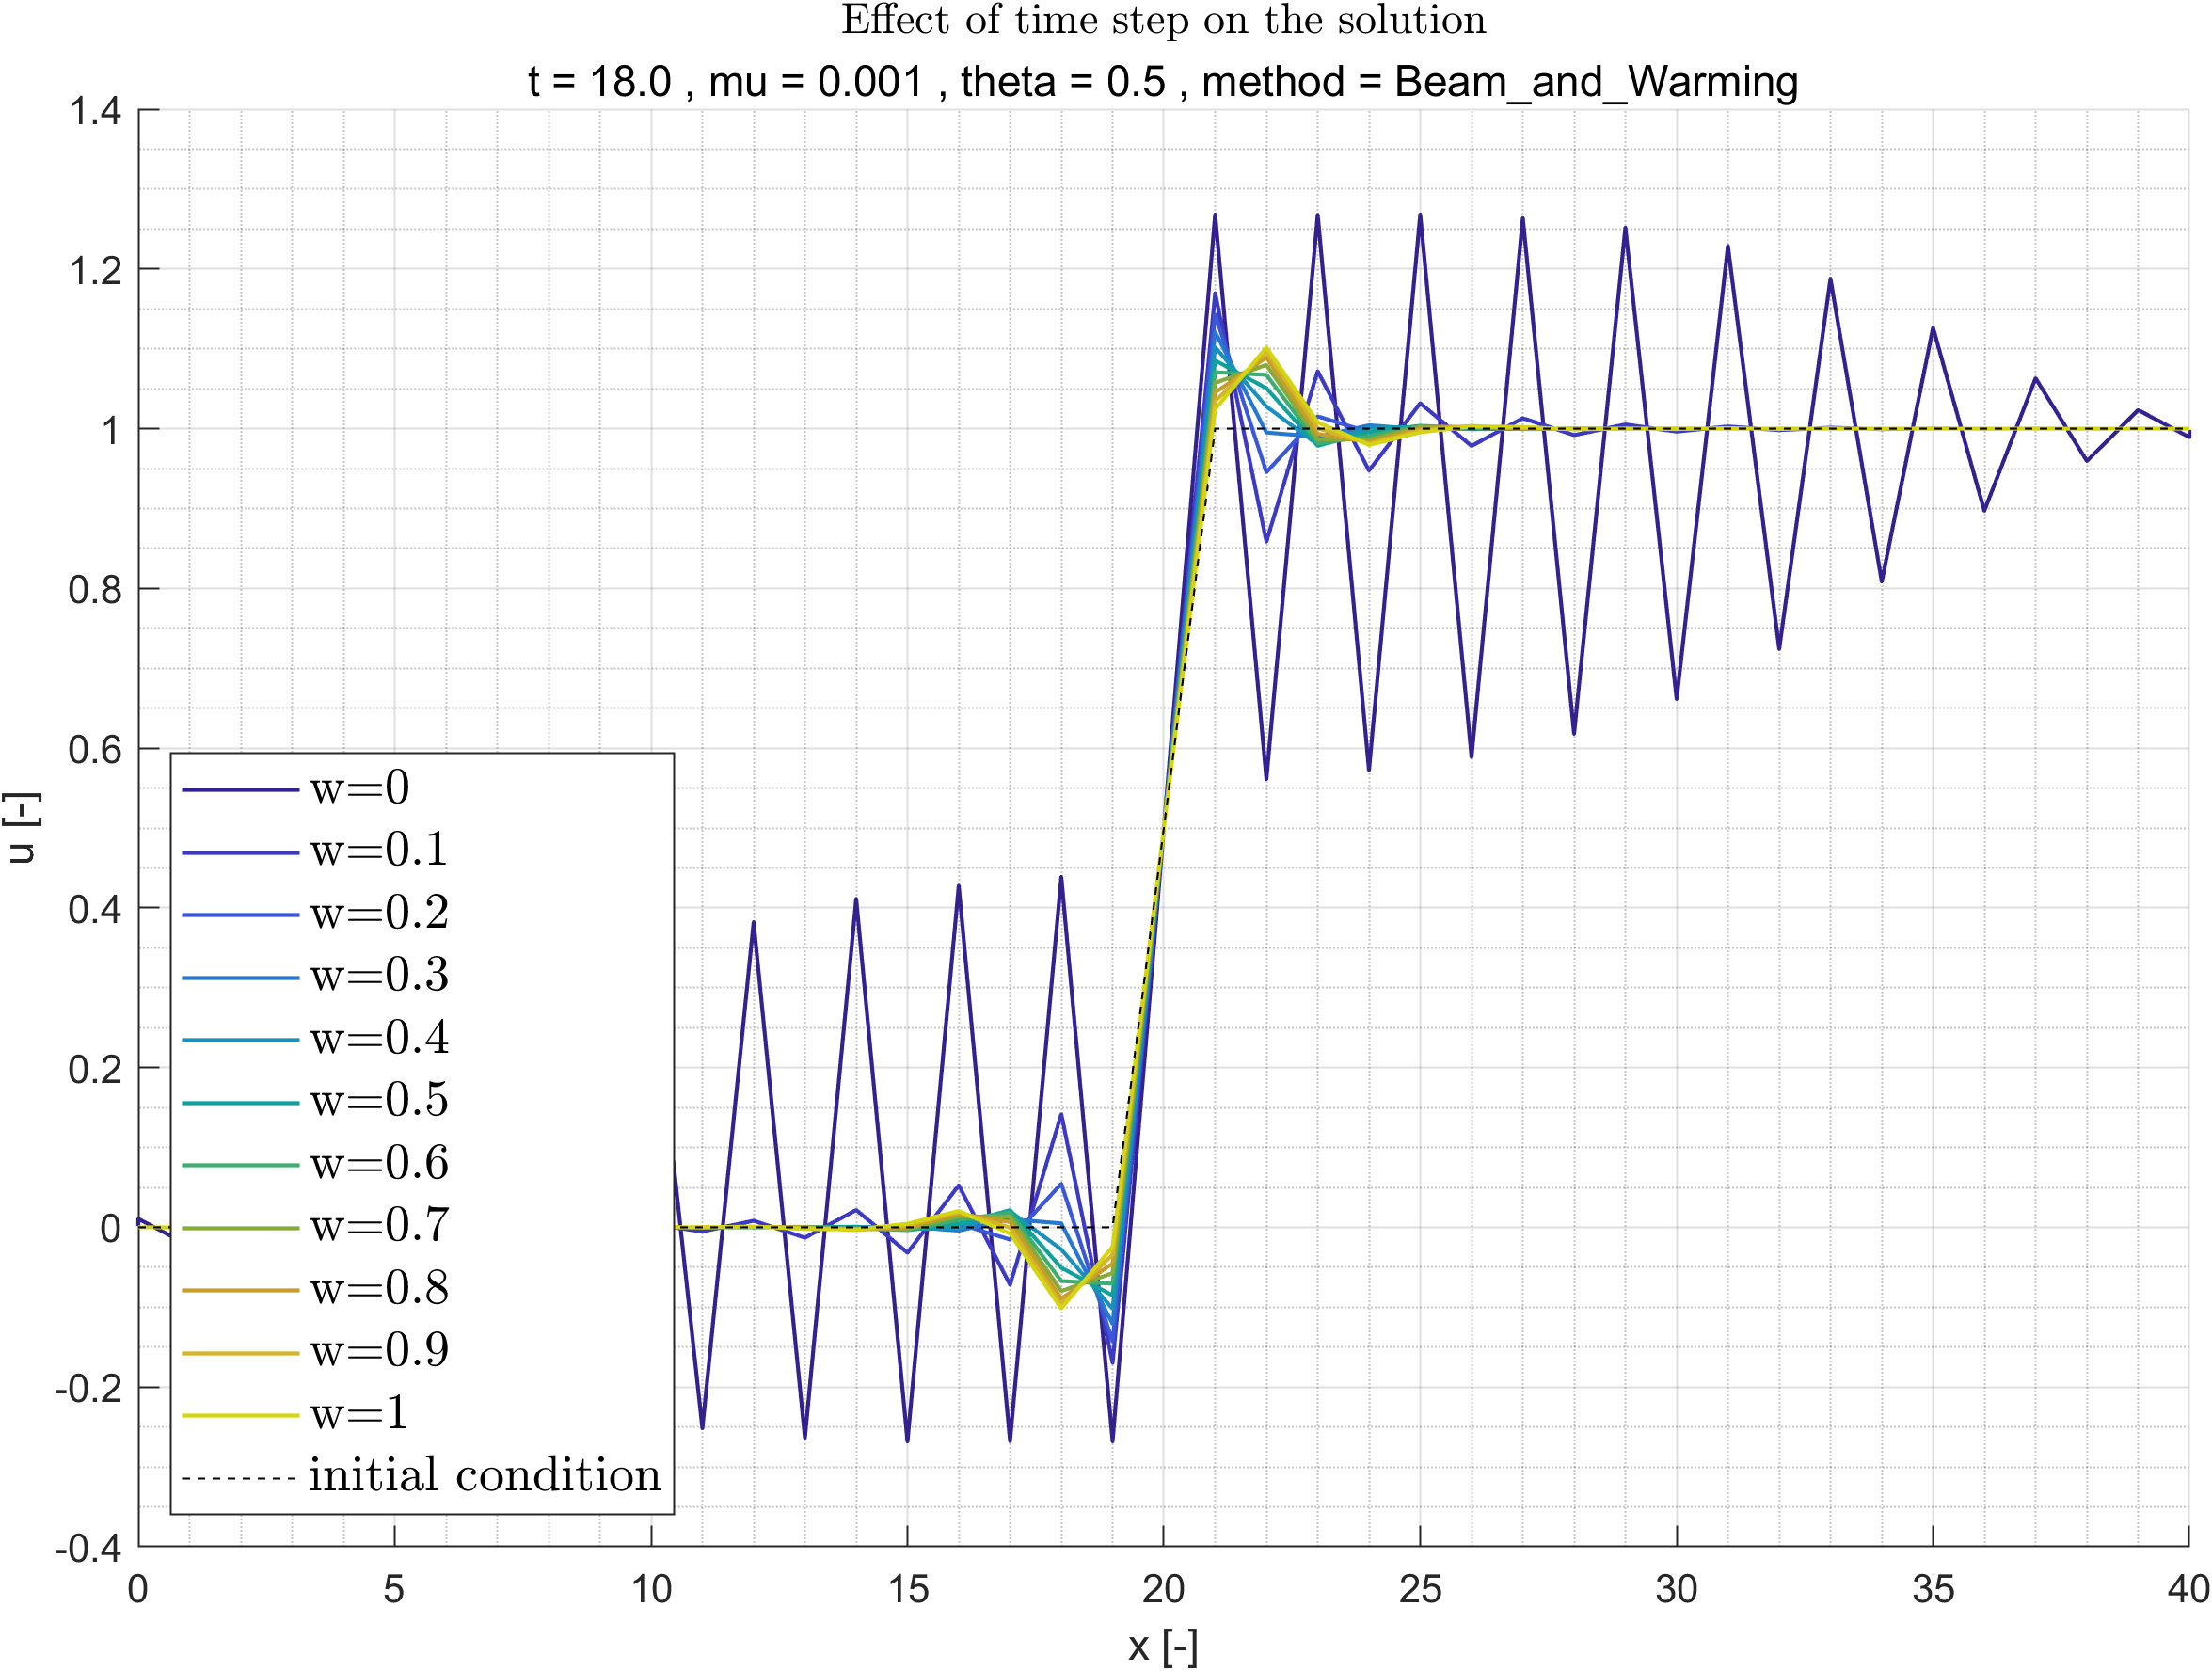
\includegraphics[width=\textwidth]{images/grap17.png}
        \caption{Beam $\&$ Warming $\mu=0.001,\ \theta=0.5$}
        \label{fig:Beam & Warming_general_mu0.001_theta0.5_A_diff_w}
    \end{subfigure}
    % \hfill
    \begin{subfigure}[c]{.38\textwidth}
        \centering
        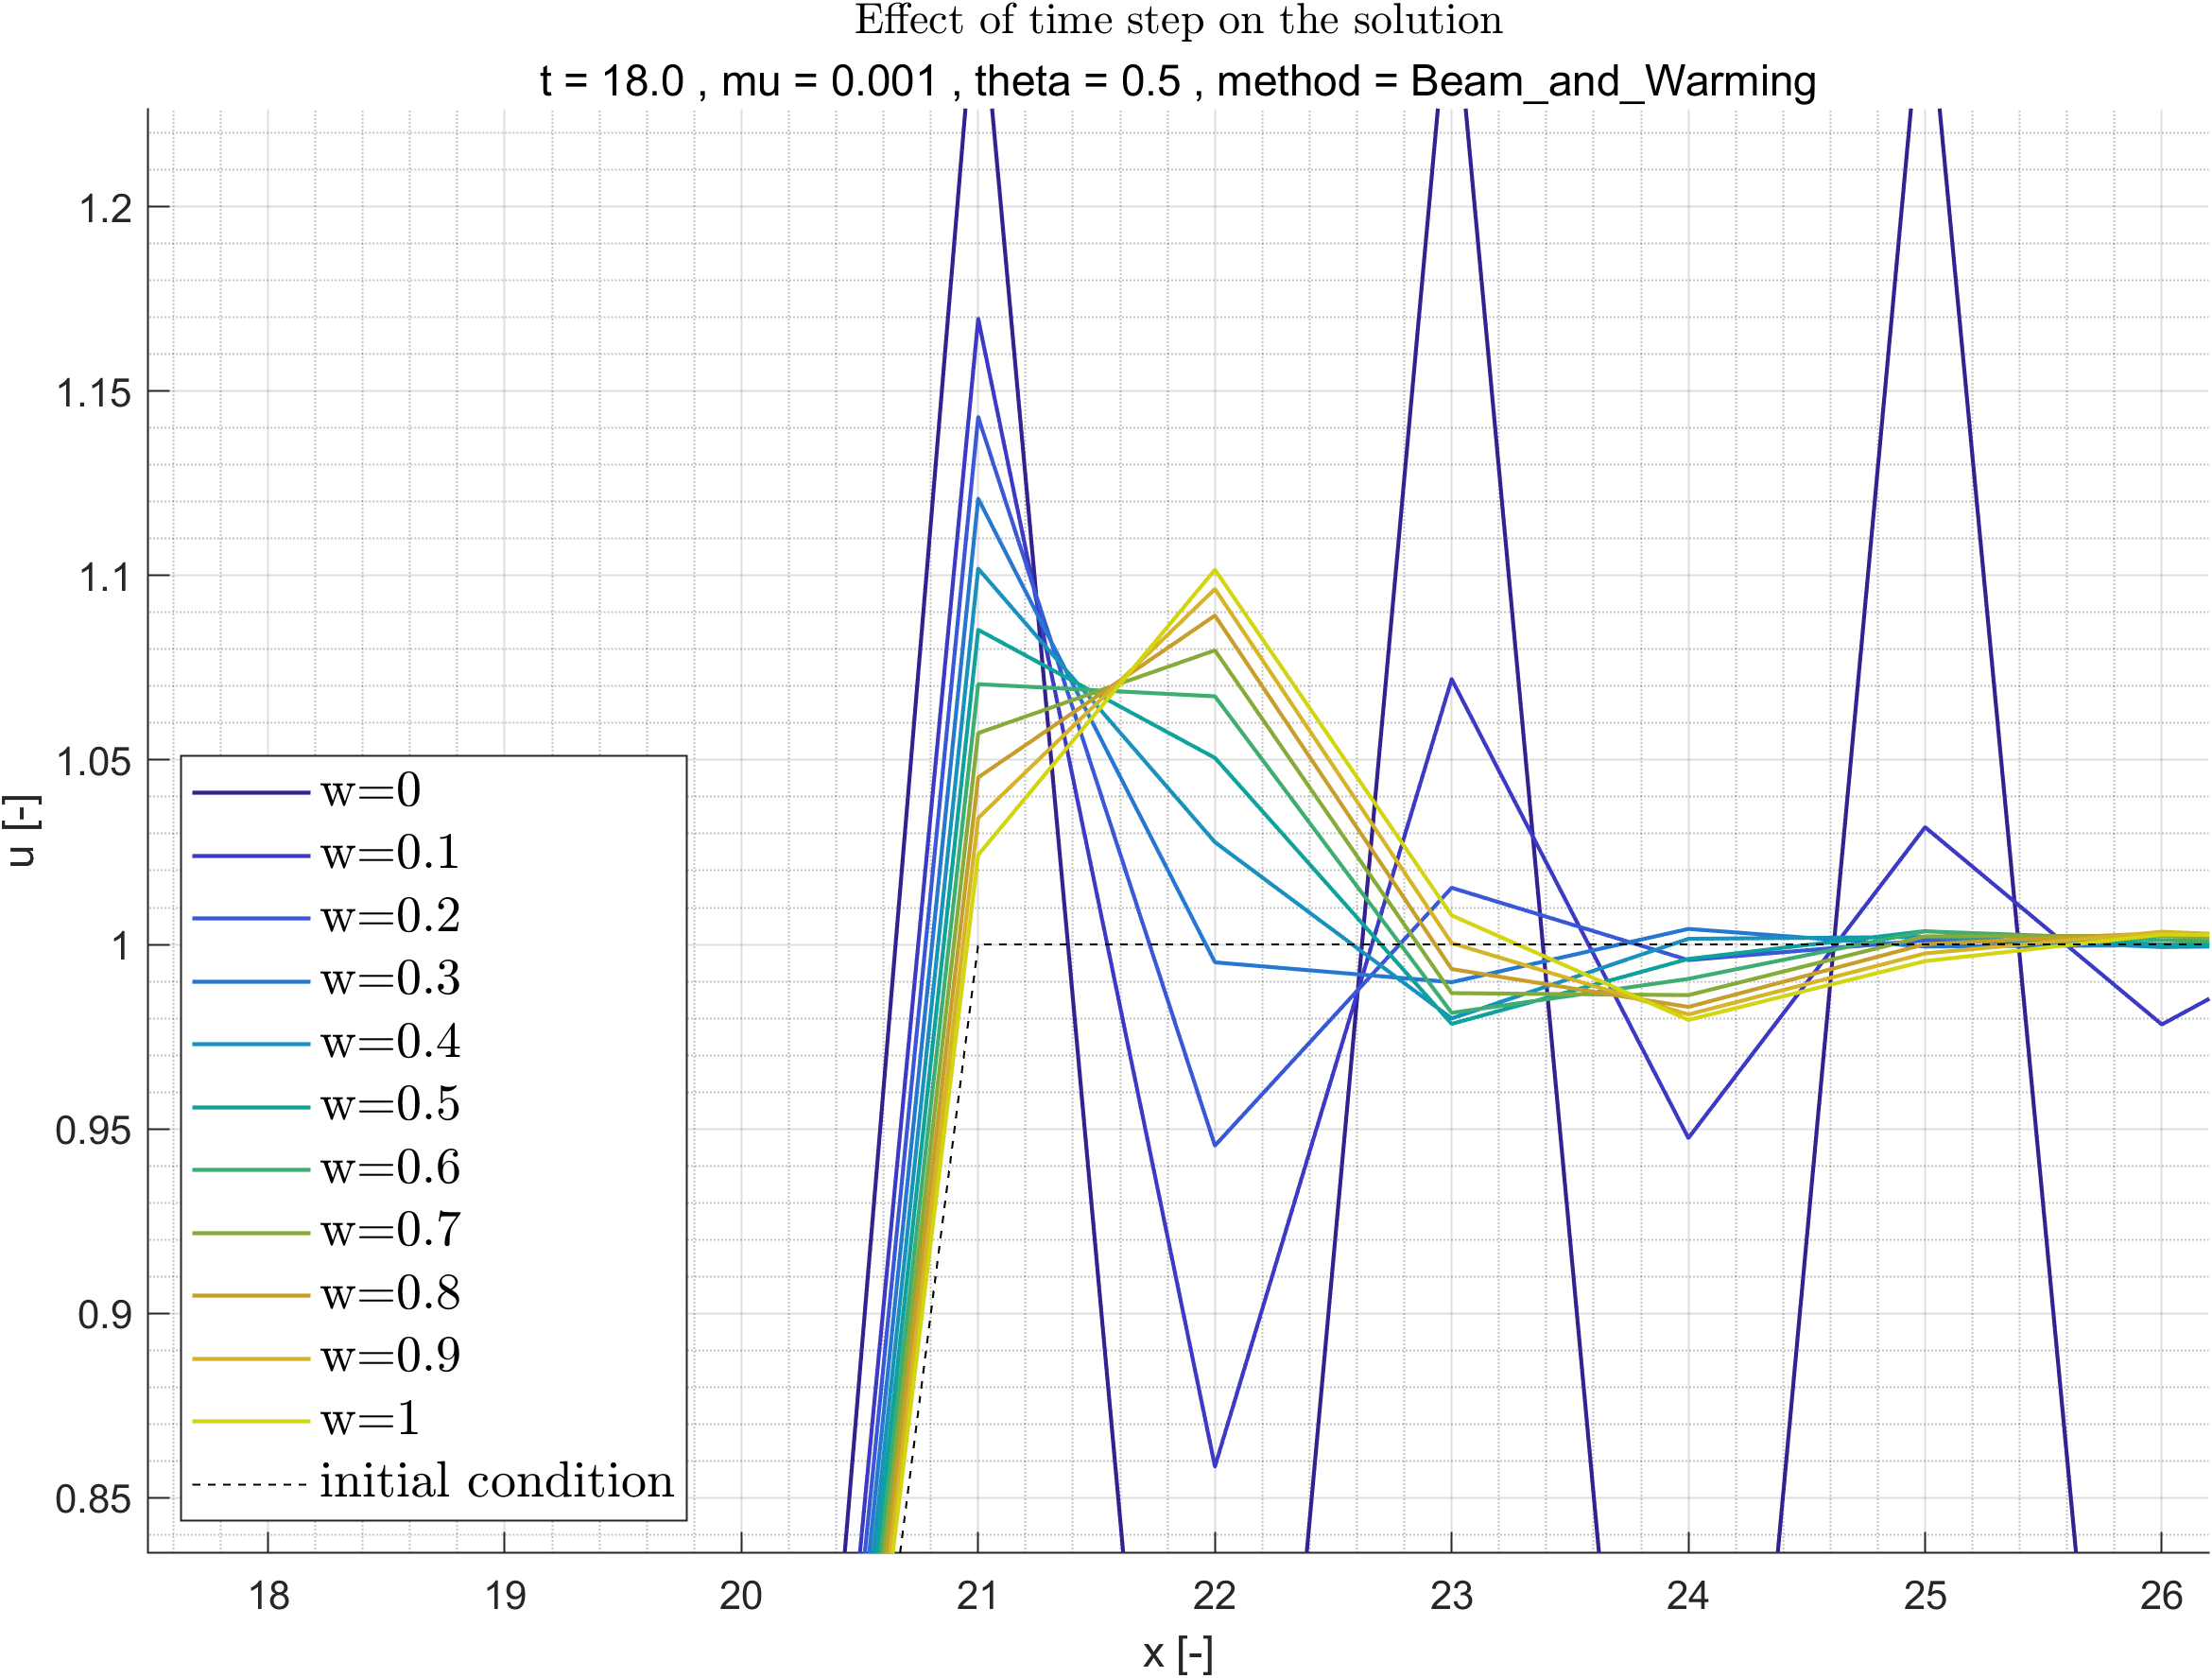
\includegraphics[width=\textwidth]{images/grap17.1.png}
        \caption{Beam $\&$ Warming $\mu=0.001,\ \theta=0.5$ - zoomed}
        \label{fig:Beam_&_Warming_general_mu0.001_theta0.5_B_diff_w}
    \end{subfigure}
    \begin{subfigure}[c]{.38\textwidth}
        \centering
        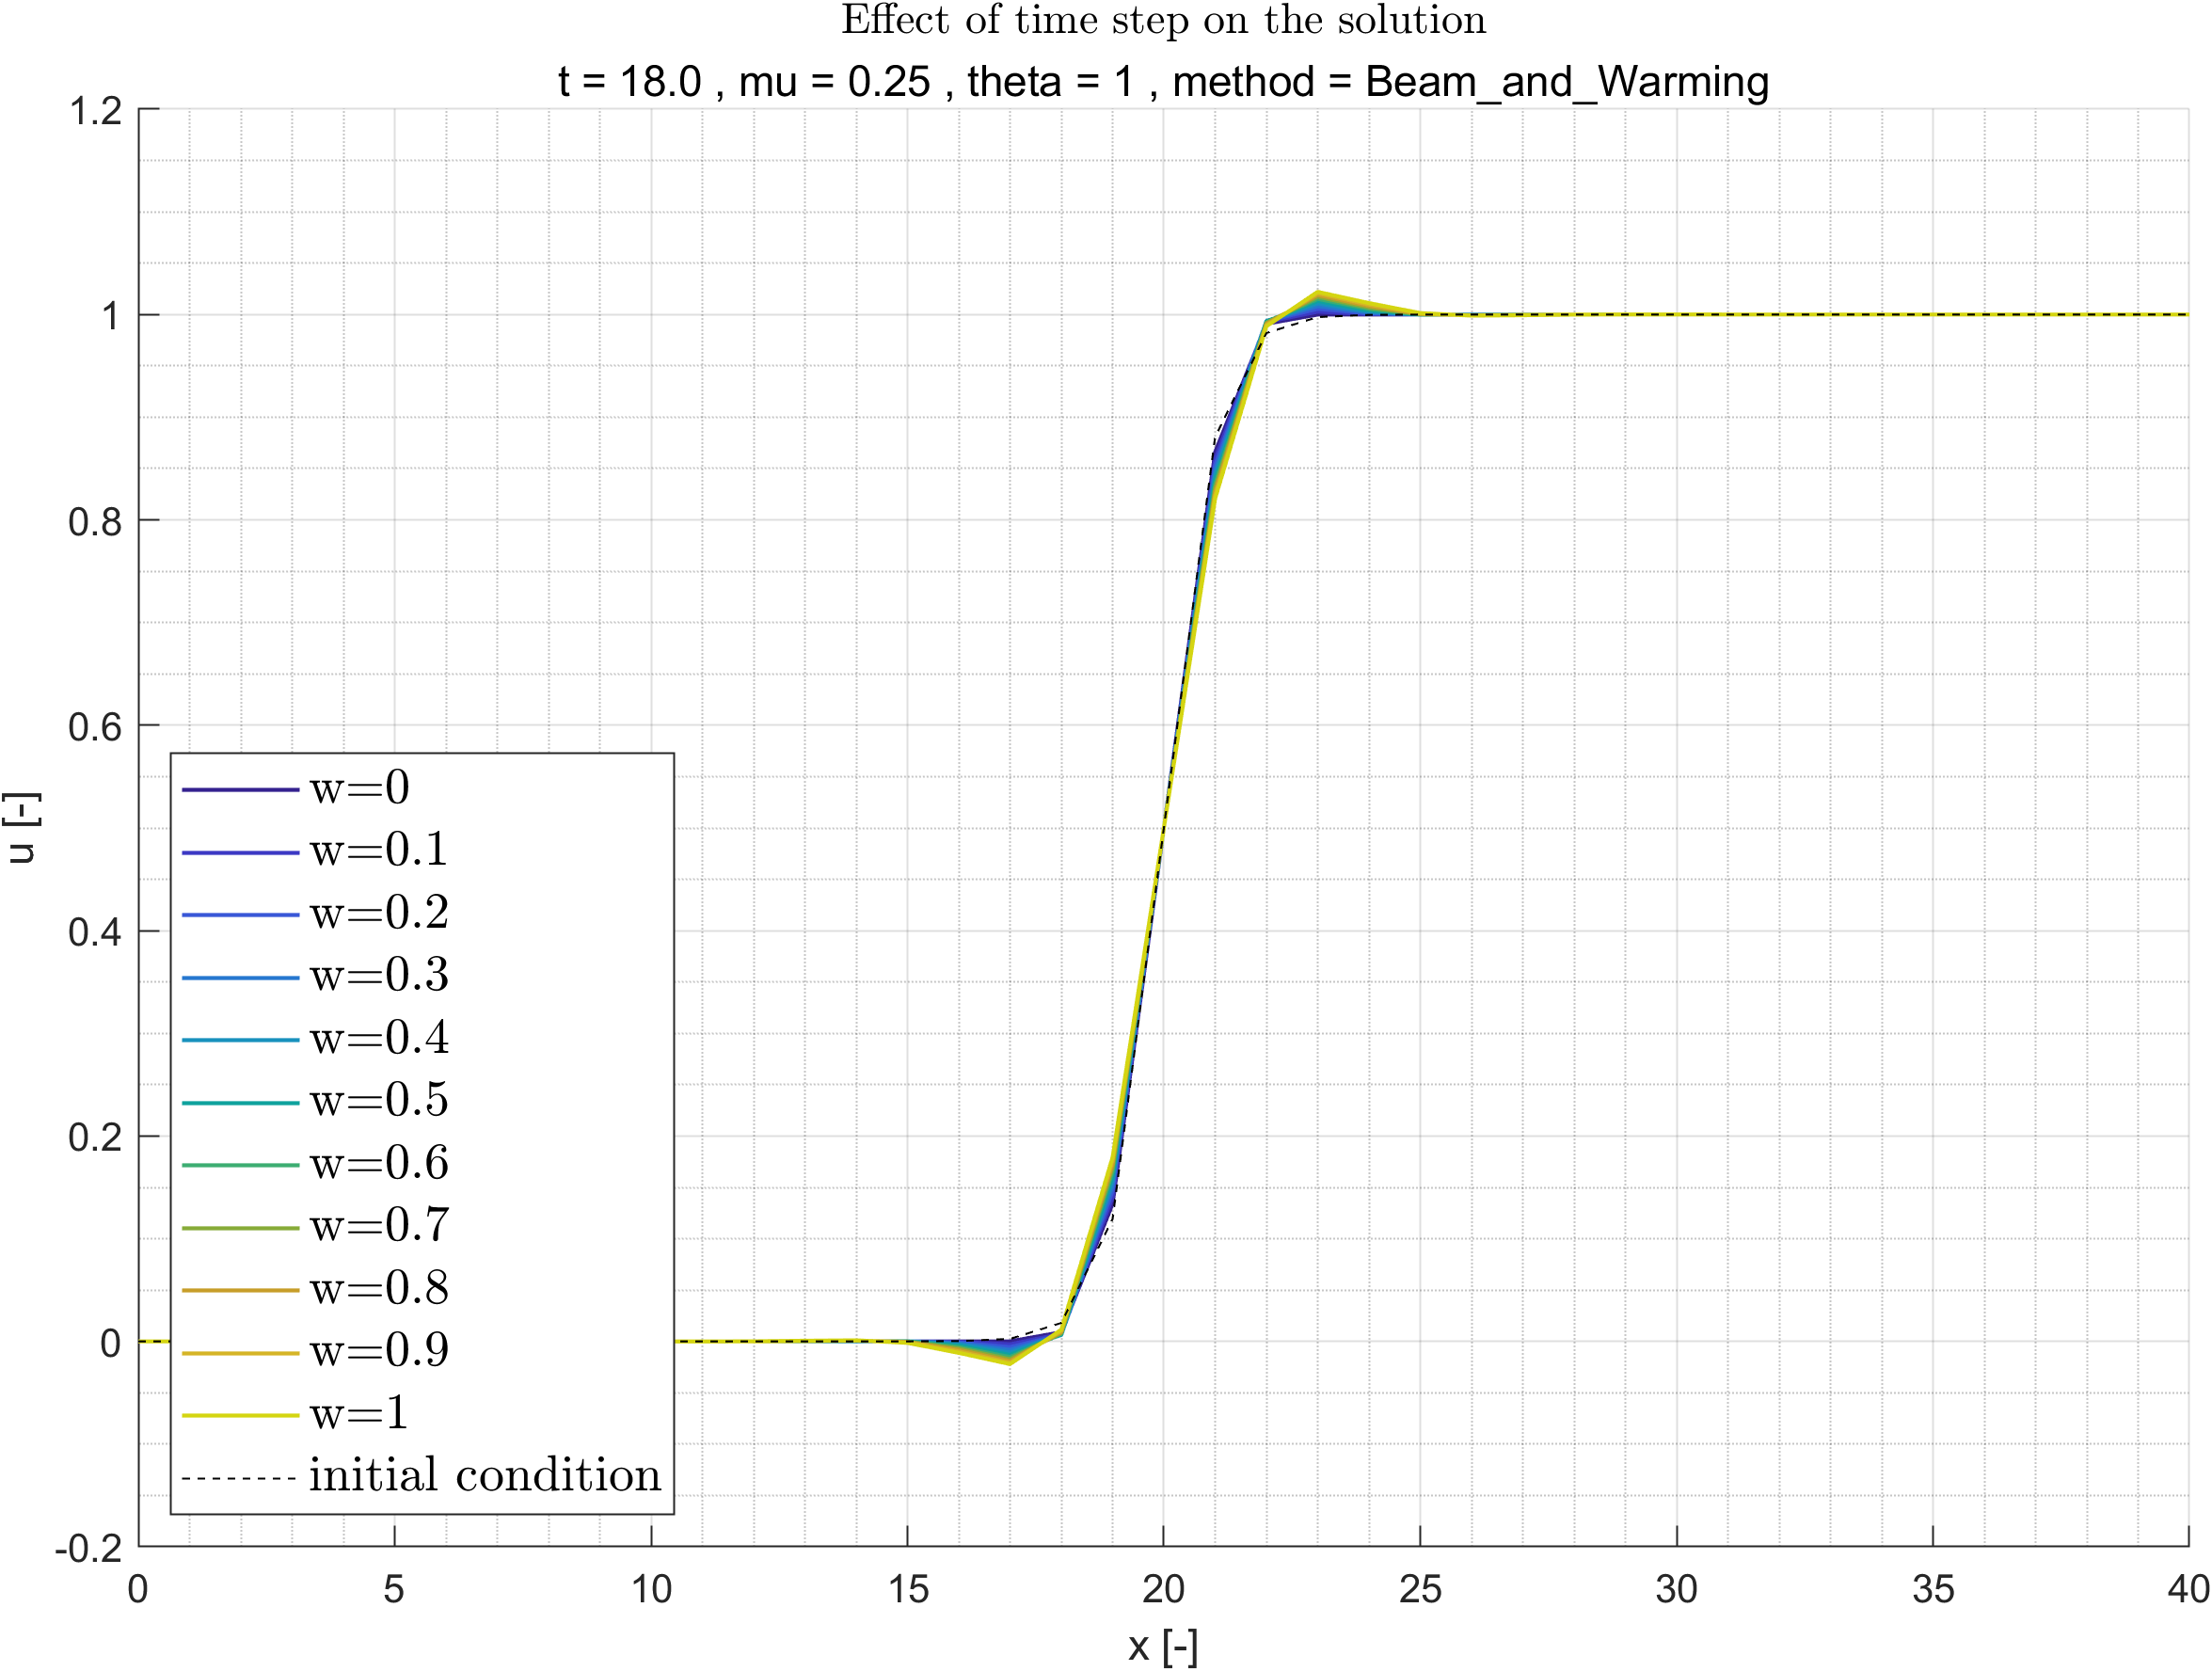
\includegraphics[width=\textwidth]{images/grap18.png}
        \caption{Beam $\&$ Warming $\mu=0.25,\ \theta=1$}
        \label{fig:Beam & Warming_general_mu0.25_theta1_A_diff_w}
    \end{subfigure}
    % \hfill
    \begin{subfigure}[c]{.38\textwidth}
        \centering
        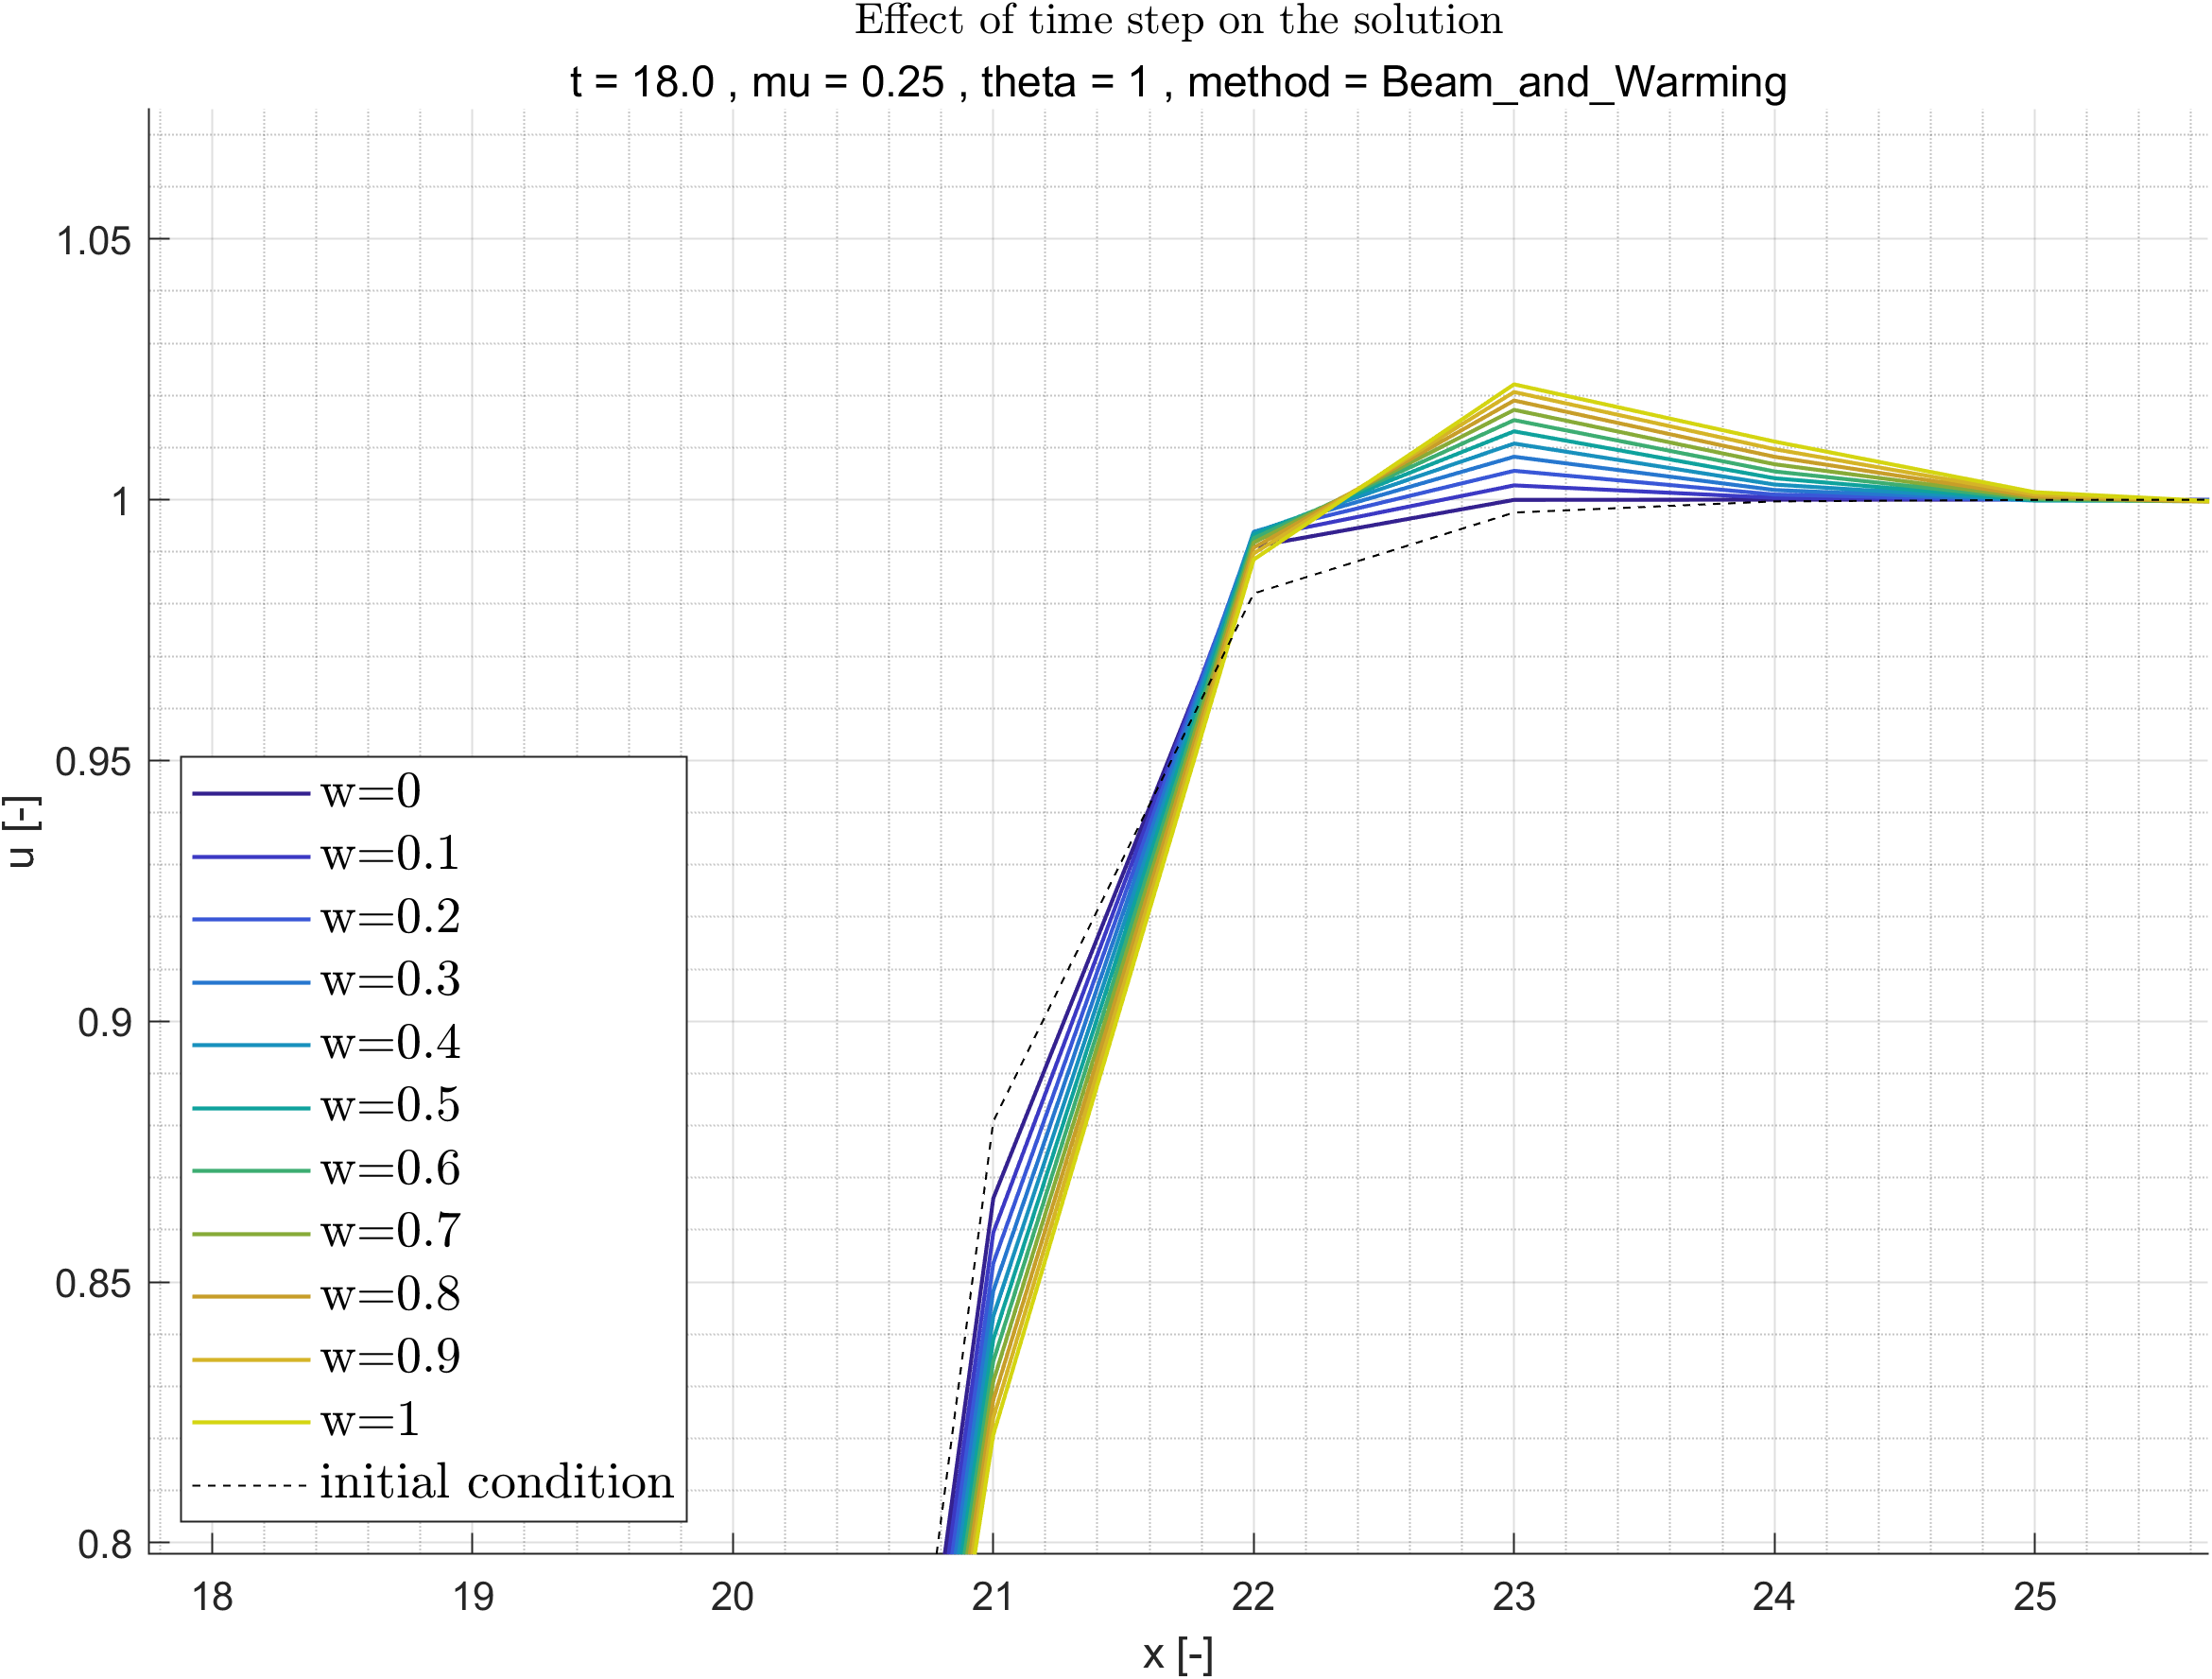
\includegraphics[width=\textwidth]{images/grap18.1.png}
        \caption{Beam $\&$ Warming $\mu=0.25,\ \theta=1$ - zoomed}
        \label{fig:Beam & Warming_general_mu0.25_theta1_B_diff_w}
    \end{subfigure}
    \begin{subfigure}[c]{.38\textwidth}
        \centering
        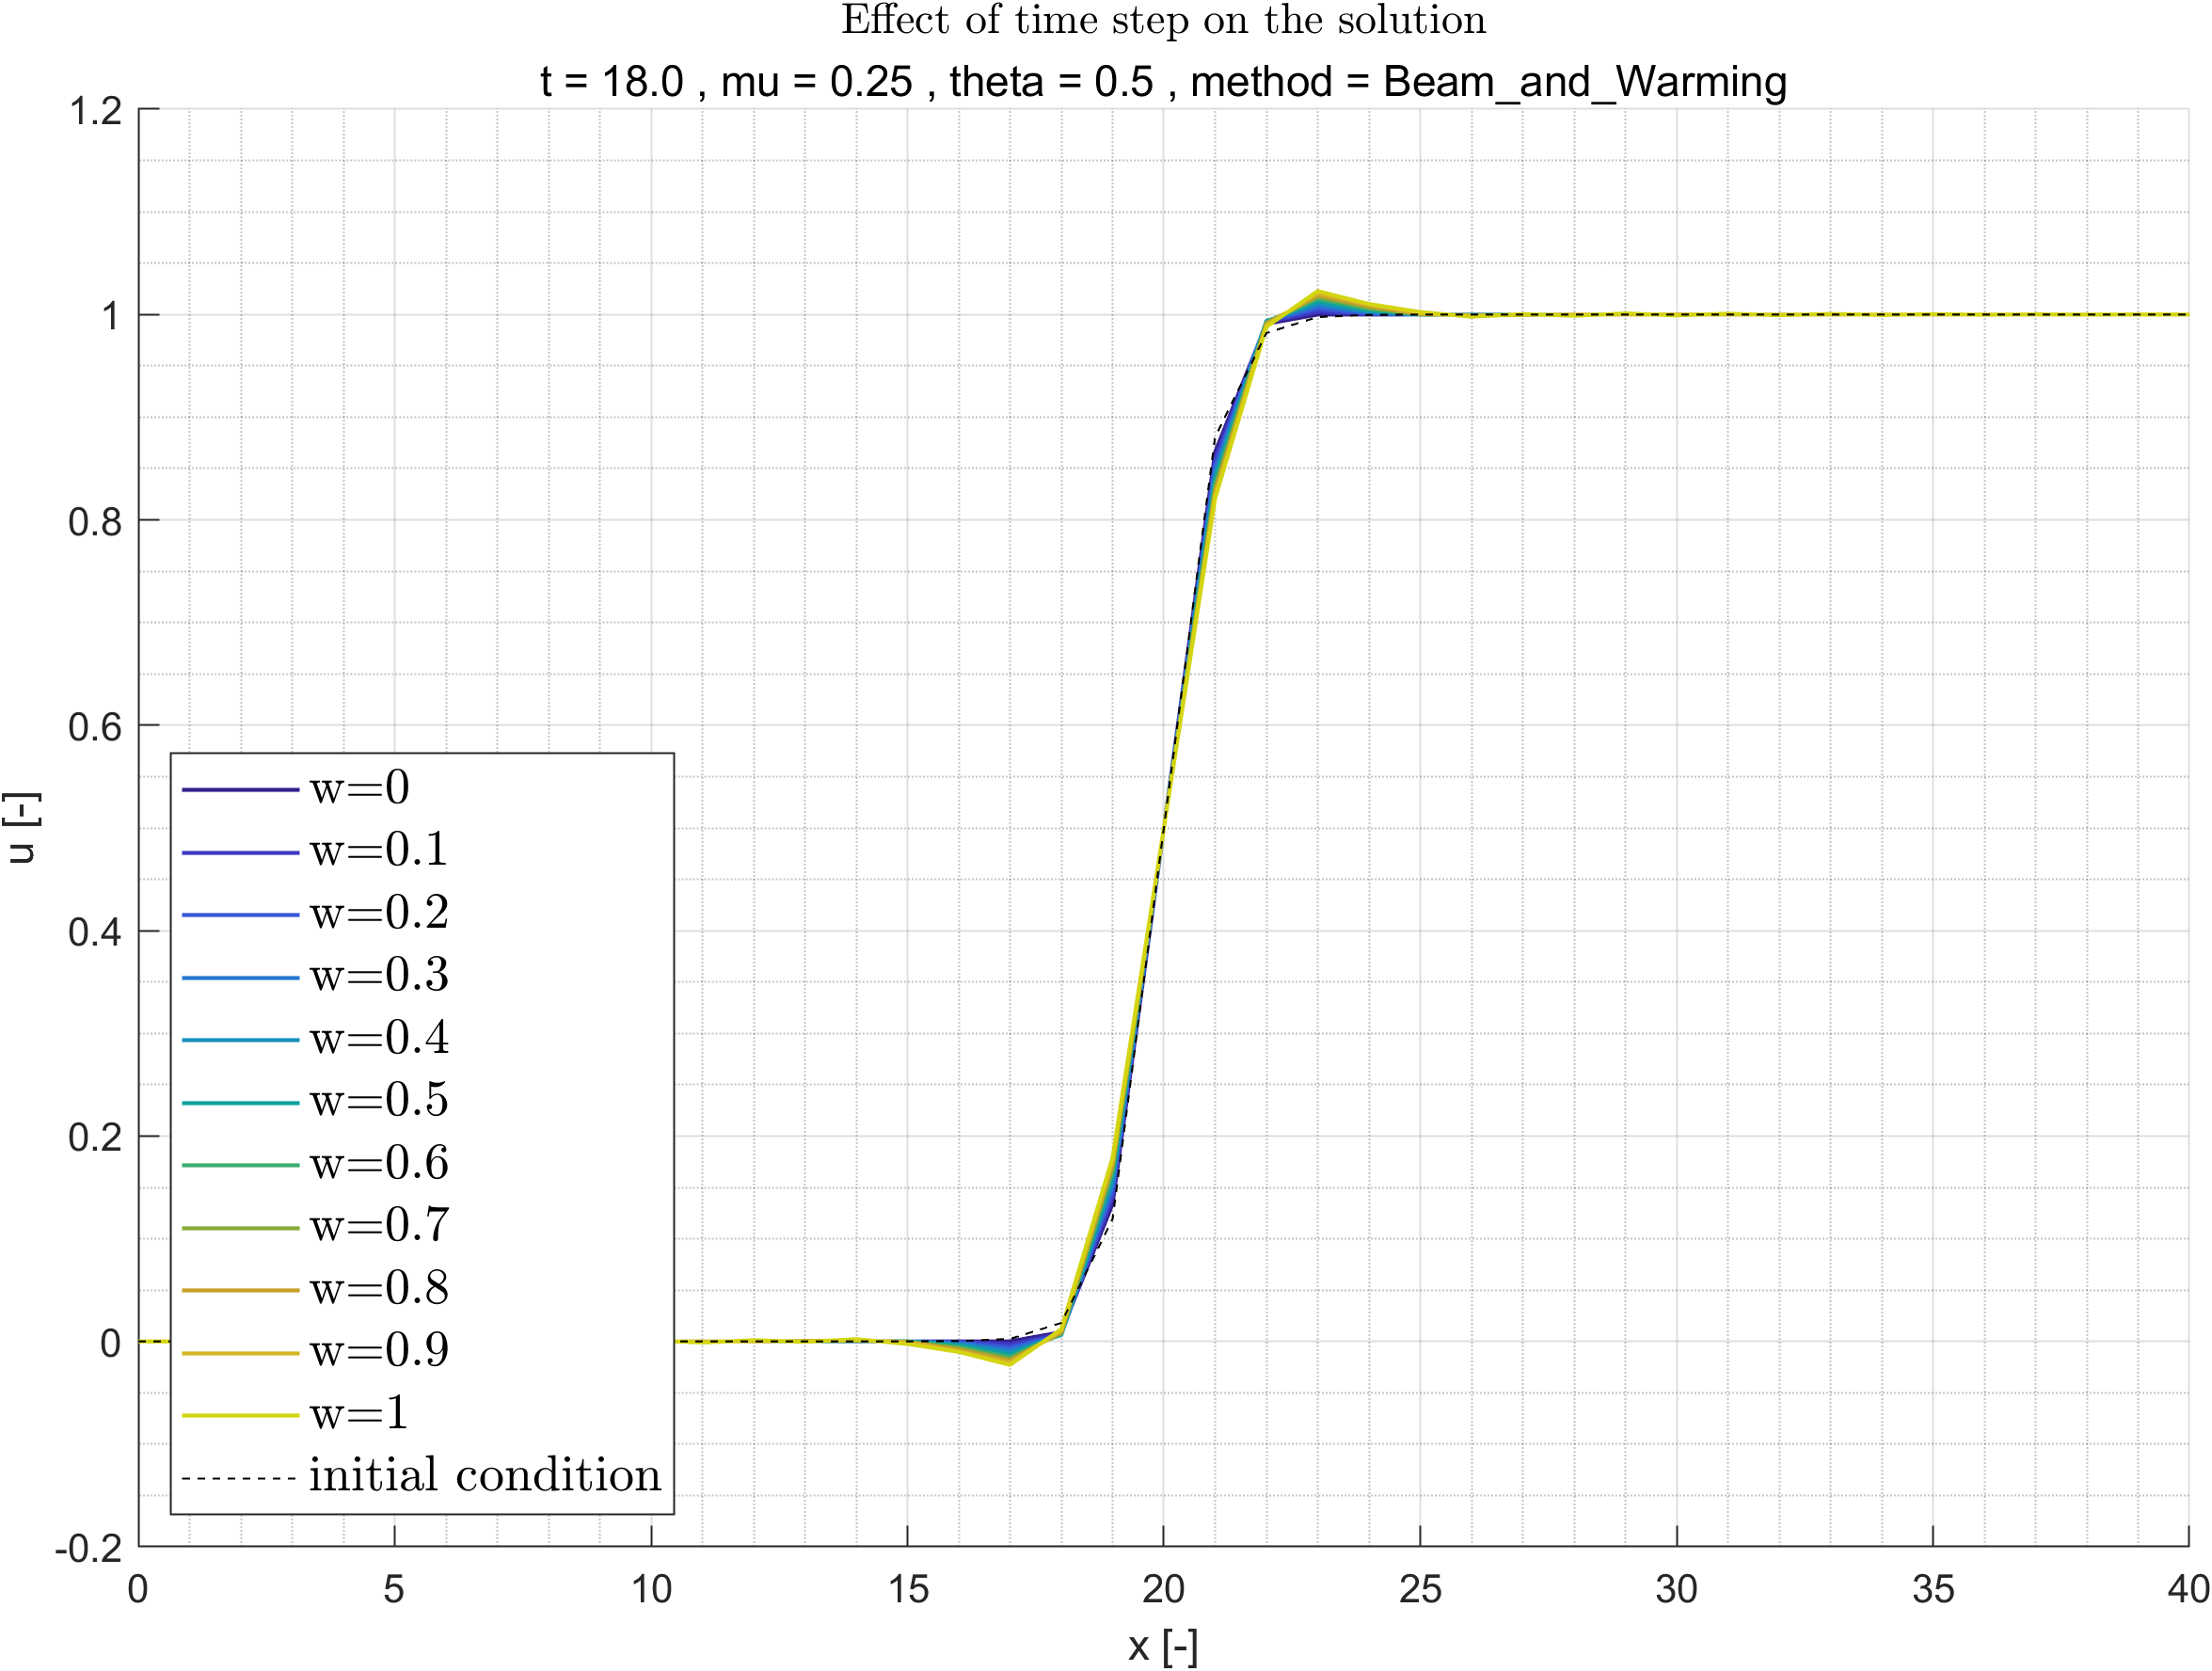
\includegraphics[width=\textwidth]{images/grap19.png}
        \caption{Beam $\&$ Warming $\mu=0.25,\ \theta=0.5$}
        \label{fig:Beam & Warming_general_mu0.25_theta0.5_A_diff_w}
    \end{subfigure}
    % \hfill
    \begin{subfigure}[c]{.38\textwidth}
        \centering
        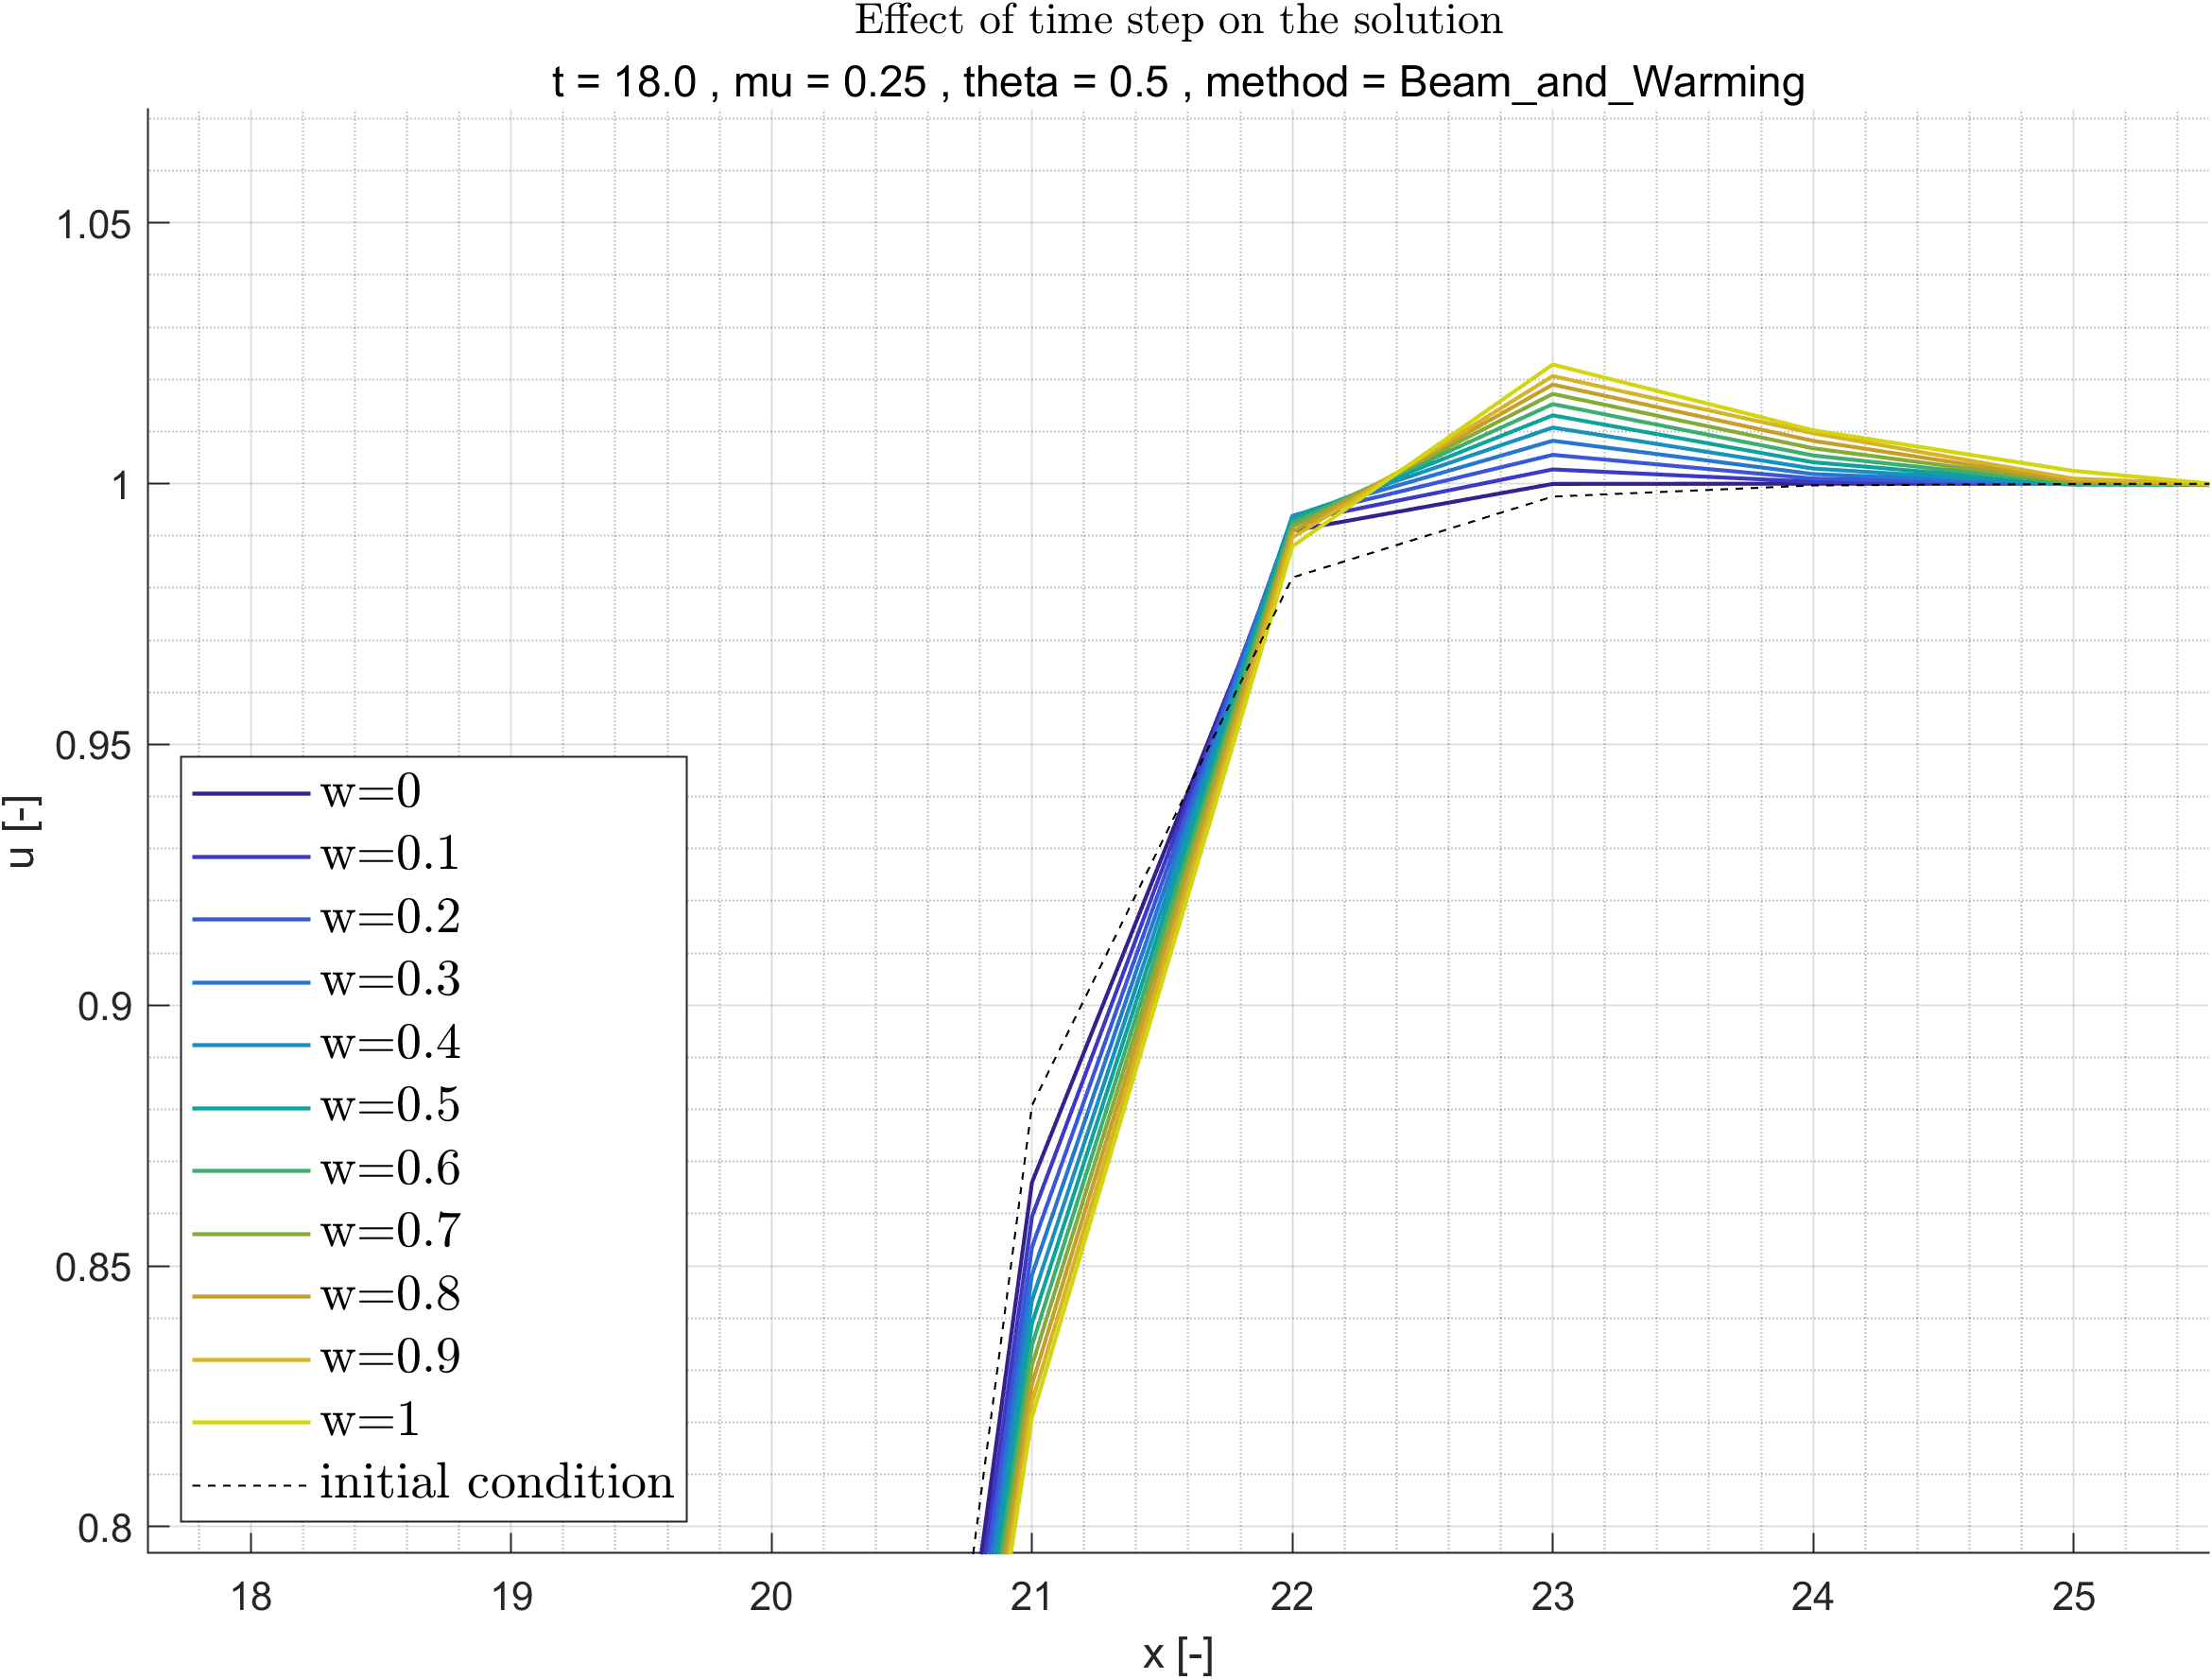
\includegraphics[width=\textwidth]{images/grap19.1.png}
        \caption{Beam $\&$ Warming $\mu=0.25,\ \theta=0.5$ - zoomed}
        \label{fig:Beam_&_Warming_general_mu0.25_theta0.5_B_diff_w}
    \end{subfigure}
    \caption{Effect of smoothing on solution - Beam $\&$ Warming}
        \label{fig:Beam_&_Warming_general_diff_w}
\end{figure}
We can see that the smoothing has a visible effect on the solution especially  significant when the viscosity is negligible. From Figure \ref{fig:Beam_&_Warming_general_diff_w} we can assume that the B$\&$W method needs smoothing in order to converge on a solution. When the viscosity $\left(\mu\right)$ and the artificial viscosity $\left(w\right)$ are negligible, the oscillations are significantly large but when only the artificial viscosity is zero, there are near to no oscillations. And again, it is visible that there is no visible difference between first order $\left(\theta=1\right)$ and second order $\left(\theta=0.5\right)$.

\subsubsection{Difference Between First and Second Order}
From the figures above (\ref{fig:Beam_&_Warming_general_diff_time} and \ref{fig:Beam_&_Warming_general_diff_w}) one might assume that there is no difference between B$\&$W first and second order. However, this assumption is obviously inaccurate at best and the next figure will show it.
\begin{figure}[H]
    \centering
    \begin{subfigure}[c]{\textwidth}
        \centering
        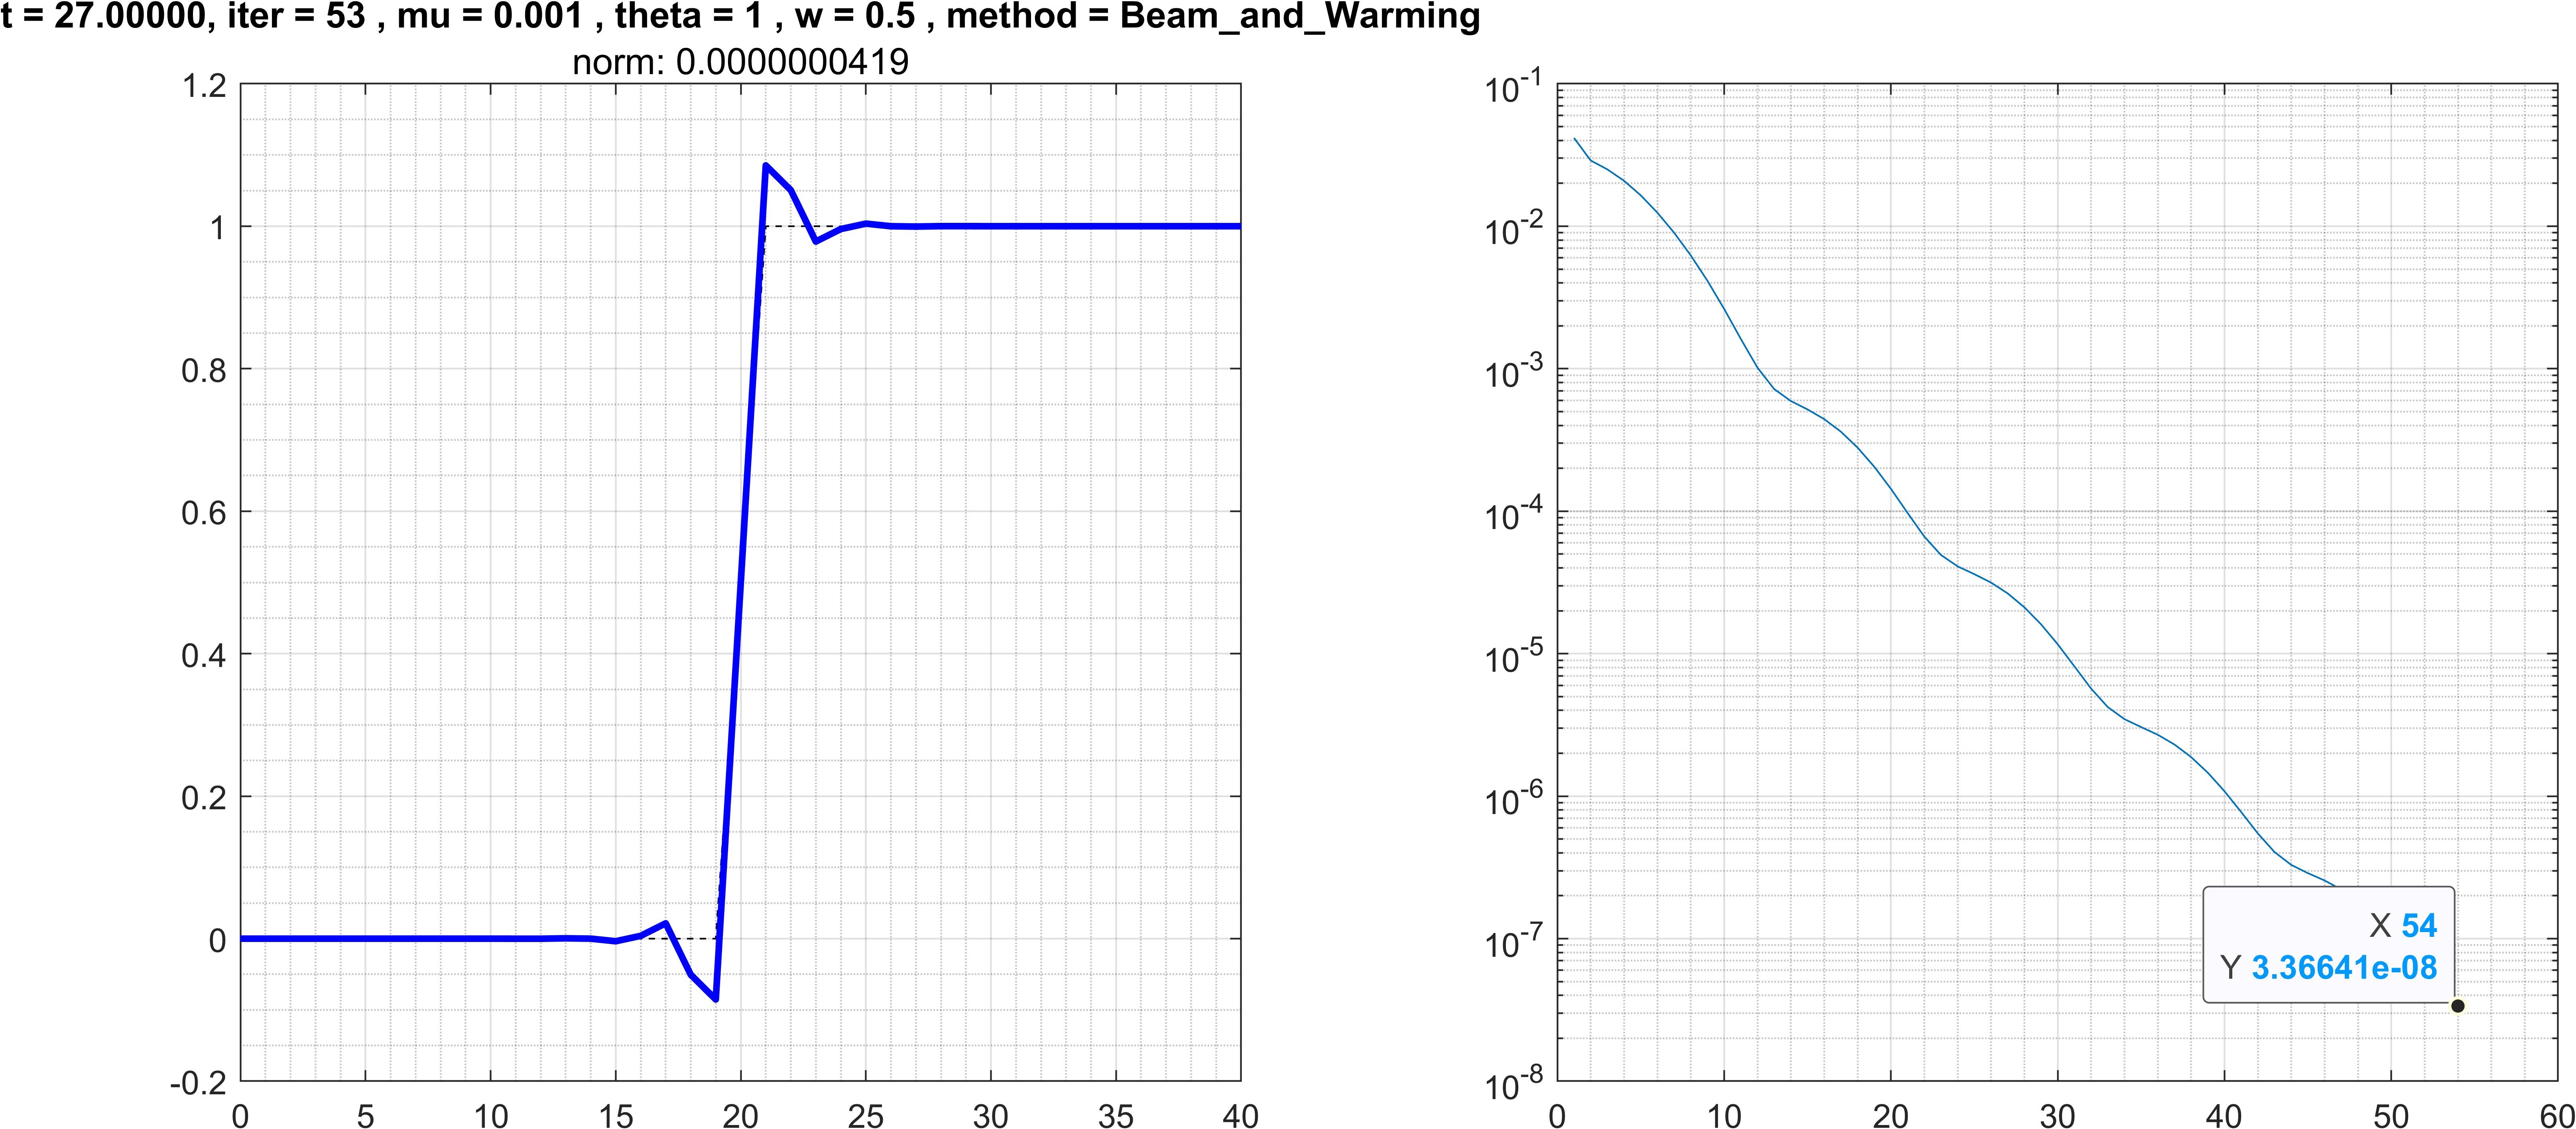
\includegraphics[width=\textwidth]{images/B&W first.png}
        \caption{Beam and Warming first order}
        \label{fig:B&W_1vs2_A}
    \end{subfigure}
    \hfill
    \begin{subfigure}[c]{\textwidth}
        \centering
        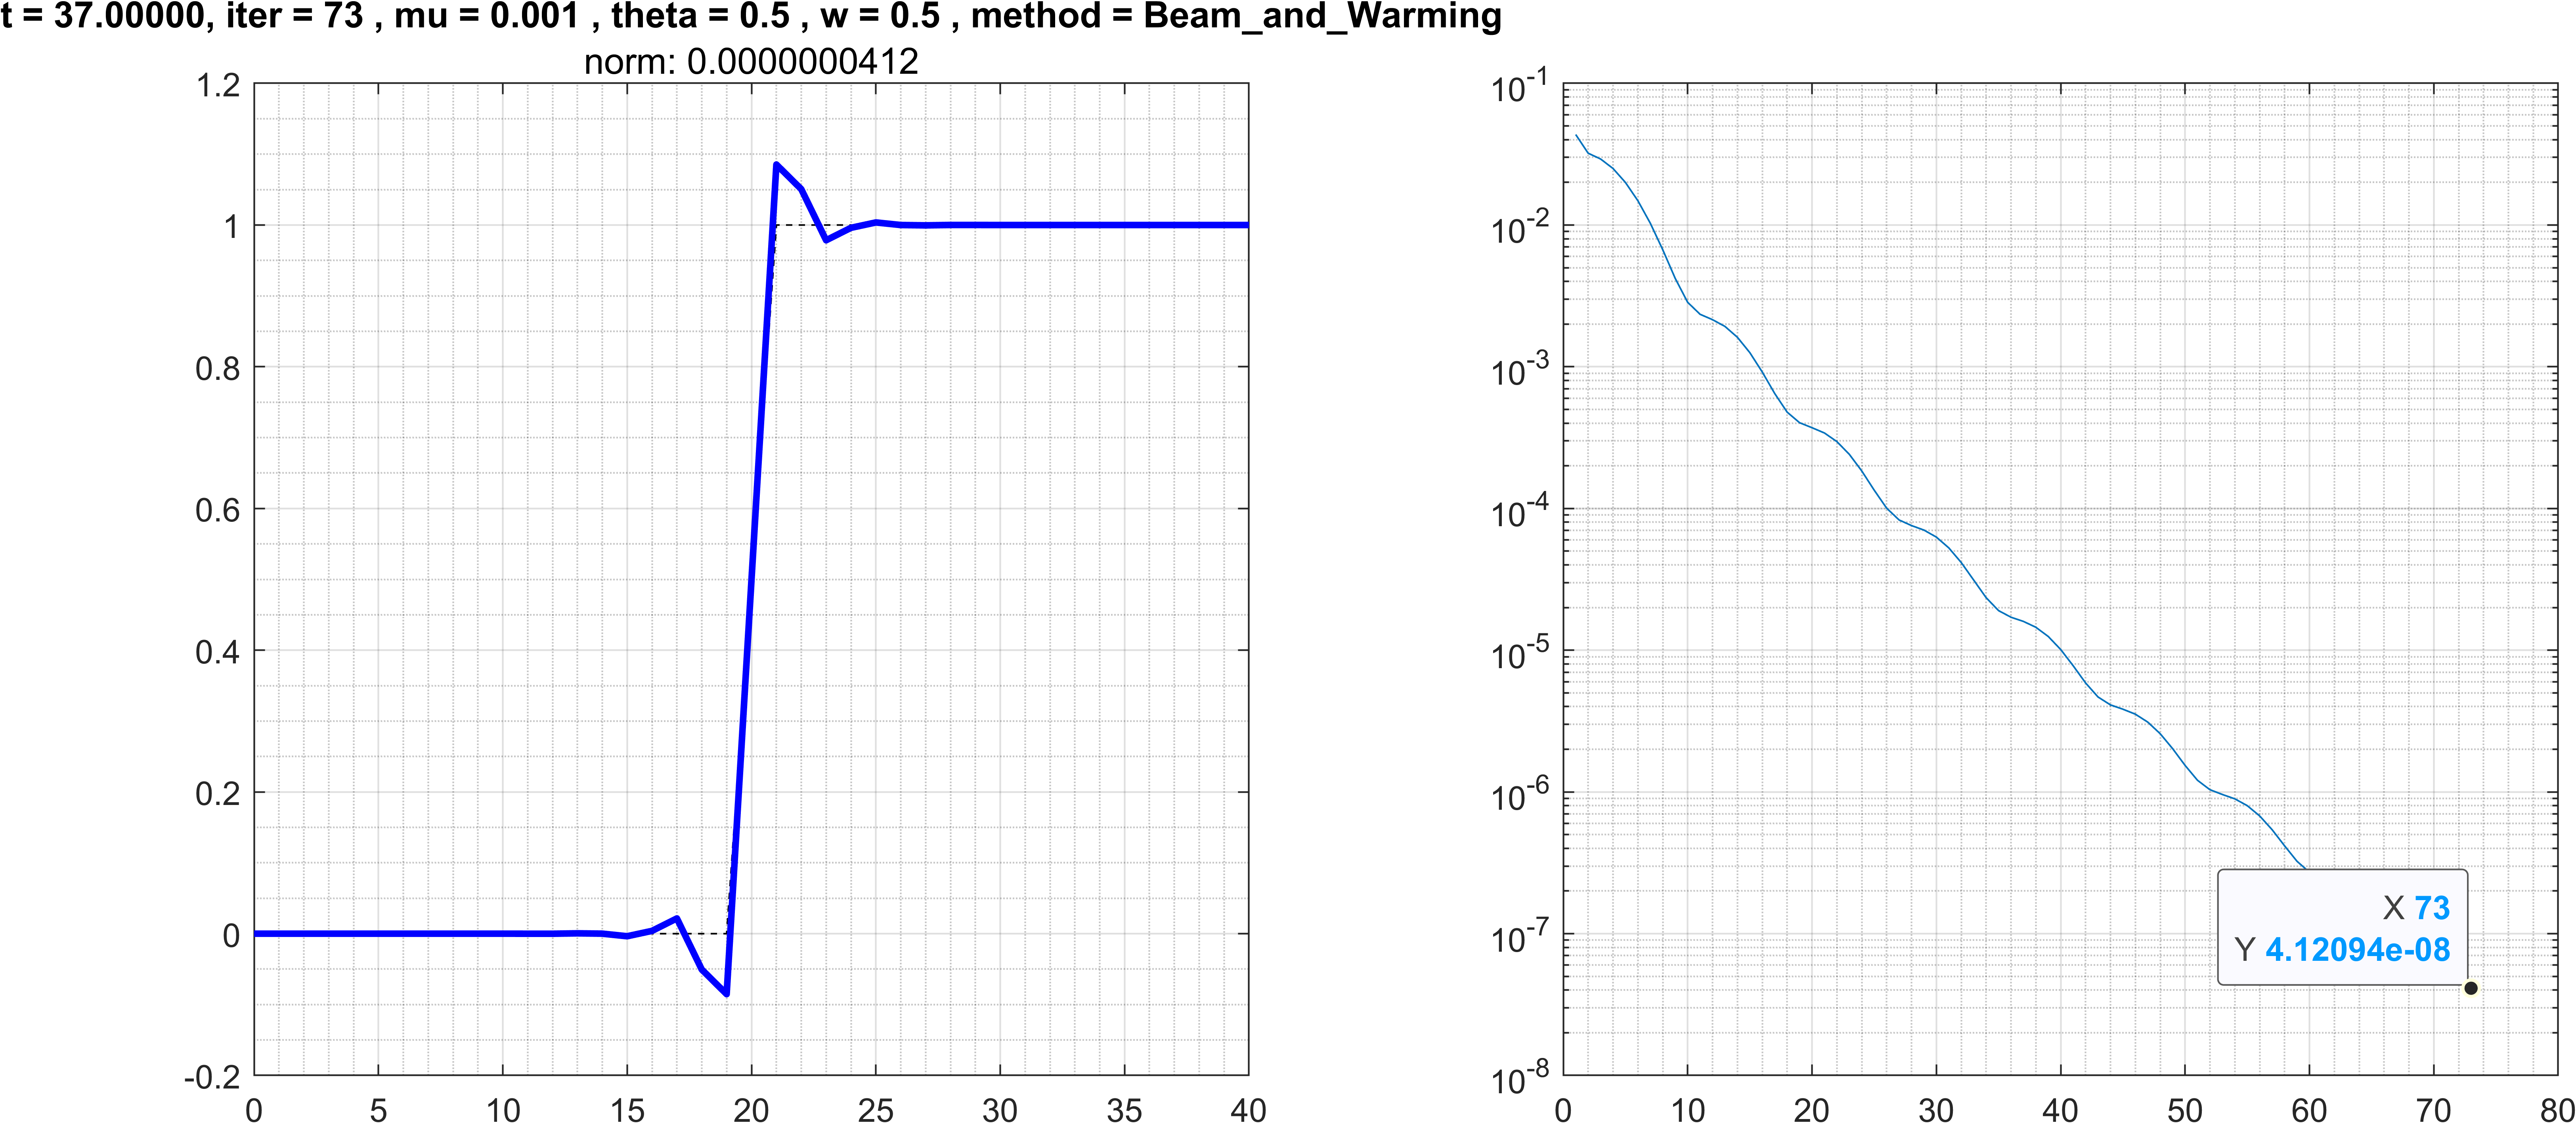
\includegraphics[width=\textwidth]{images/B&W second.png}
        \caption{Beam and Warming second order}
        \label{fig:B&W_1vs2_B}
    \end{subfigure}
    \caption{Difference between B$\&$W first and second order}
        \label{fig:B&W_1vs2}
\end{figure}
\noindent We can see that indeed there is a difference between first and second order. First order takes less iteration to converge but the residual of the second order is smaller.

\section{Conclusions}
\subsection{Inviscid Burgers Equation}
\begin{itemize}
    \item Although the stability limit for the Roe first-order method is $\mathrm{CFL}<1$, in Figure \ref{fig:roe_first_inviscid} we can see that the method is still stable for $\mathrm{CFL}>1$. This can be explained by the fact that stability analysis can be performed only for linear equations and the Burgers equation is a non-linear equation, so it is reasonable that the method states stable for CFL numbers slightly bigger than the limitation.
    \item The Roe second-order method is less stable than the first-order and since the method is dispersive (unlike the dissipative first-order) there are oscillations for all CFL numbers (the oscillations are negligible when the CFL number is small).
    \item To limit the oscillations of the second-order, different limiters are in use. The limiters make the method stable at least like the first-order method and they delay the start of the oscillations.
    \item Each limiter has its advantages and disadvantages.
    The van Leer limiter, unlike most, keeps some small oscillations on the wavefront, and with the Supperbee limiter, the oscillations start first.
\end{itemize}

\subsection{Generalized Burgers Equation}
\begin{itemize}
    \item The effect of the time step is near negligible for the Roe first-order method.
    \item For the MacCormack and Beam $\&$ Warming methods, the time step is has nearlly negligible effect when the viscosity $\left(\mu\right)$ is high and substianal effect when the viscosity is negligible.
    \item As expected, the solution with teh MacCormack method (second-order) has oscillations around the wavefront which are more pronounced when the viscosity is negligible.
    \item Both first and second order Beam and Warming has oscillations around the wavefront. Unlike the other scheme, the time step has a visible effect for both values of viscosity.
    \item Since the B$\&$W method is highly dispersive (as seen in Figure \ref{fig:Beam_&_Warming_general_diff_w} for $\mathrm{w}=0$) an artificial viscosity $\left(\mathrm{w}\right)$ has been added. The artiricial viscosity is especially importent when the real viscosity $\left(\mu\right)$ is small. 
    \item As the artificial viscosity increase so do the oscillations near the wavefront.
\end{itemize}

\appendix
\section{Functional Description}
\subsection{Flow Chart}
\begin{figure}[H]
    \centering
    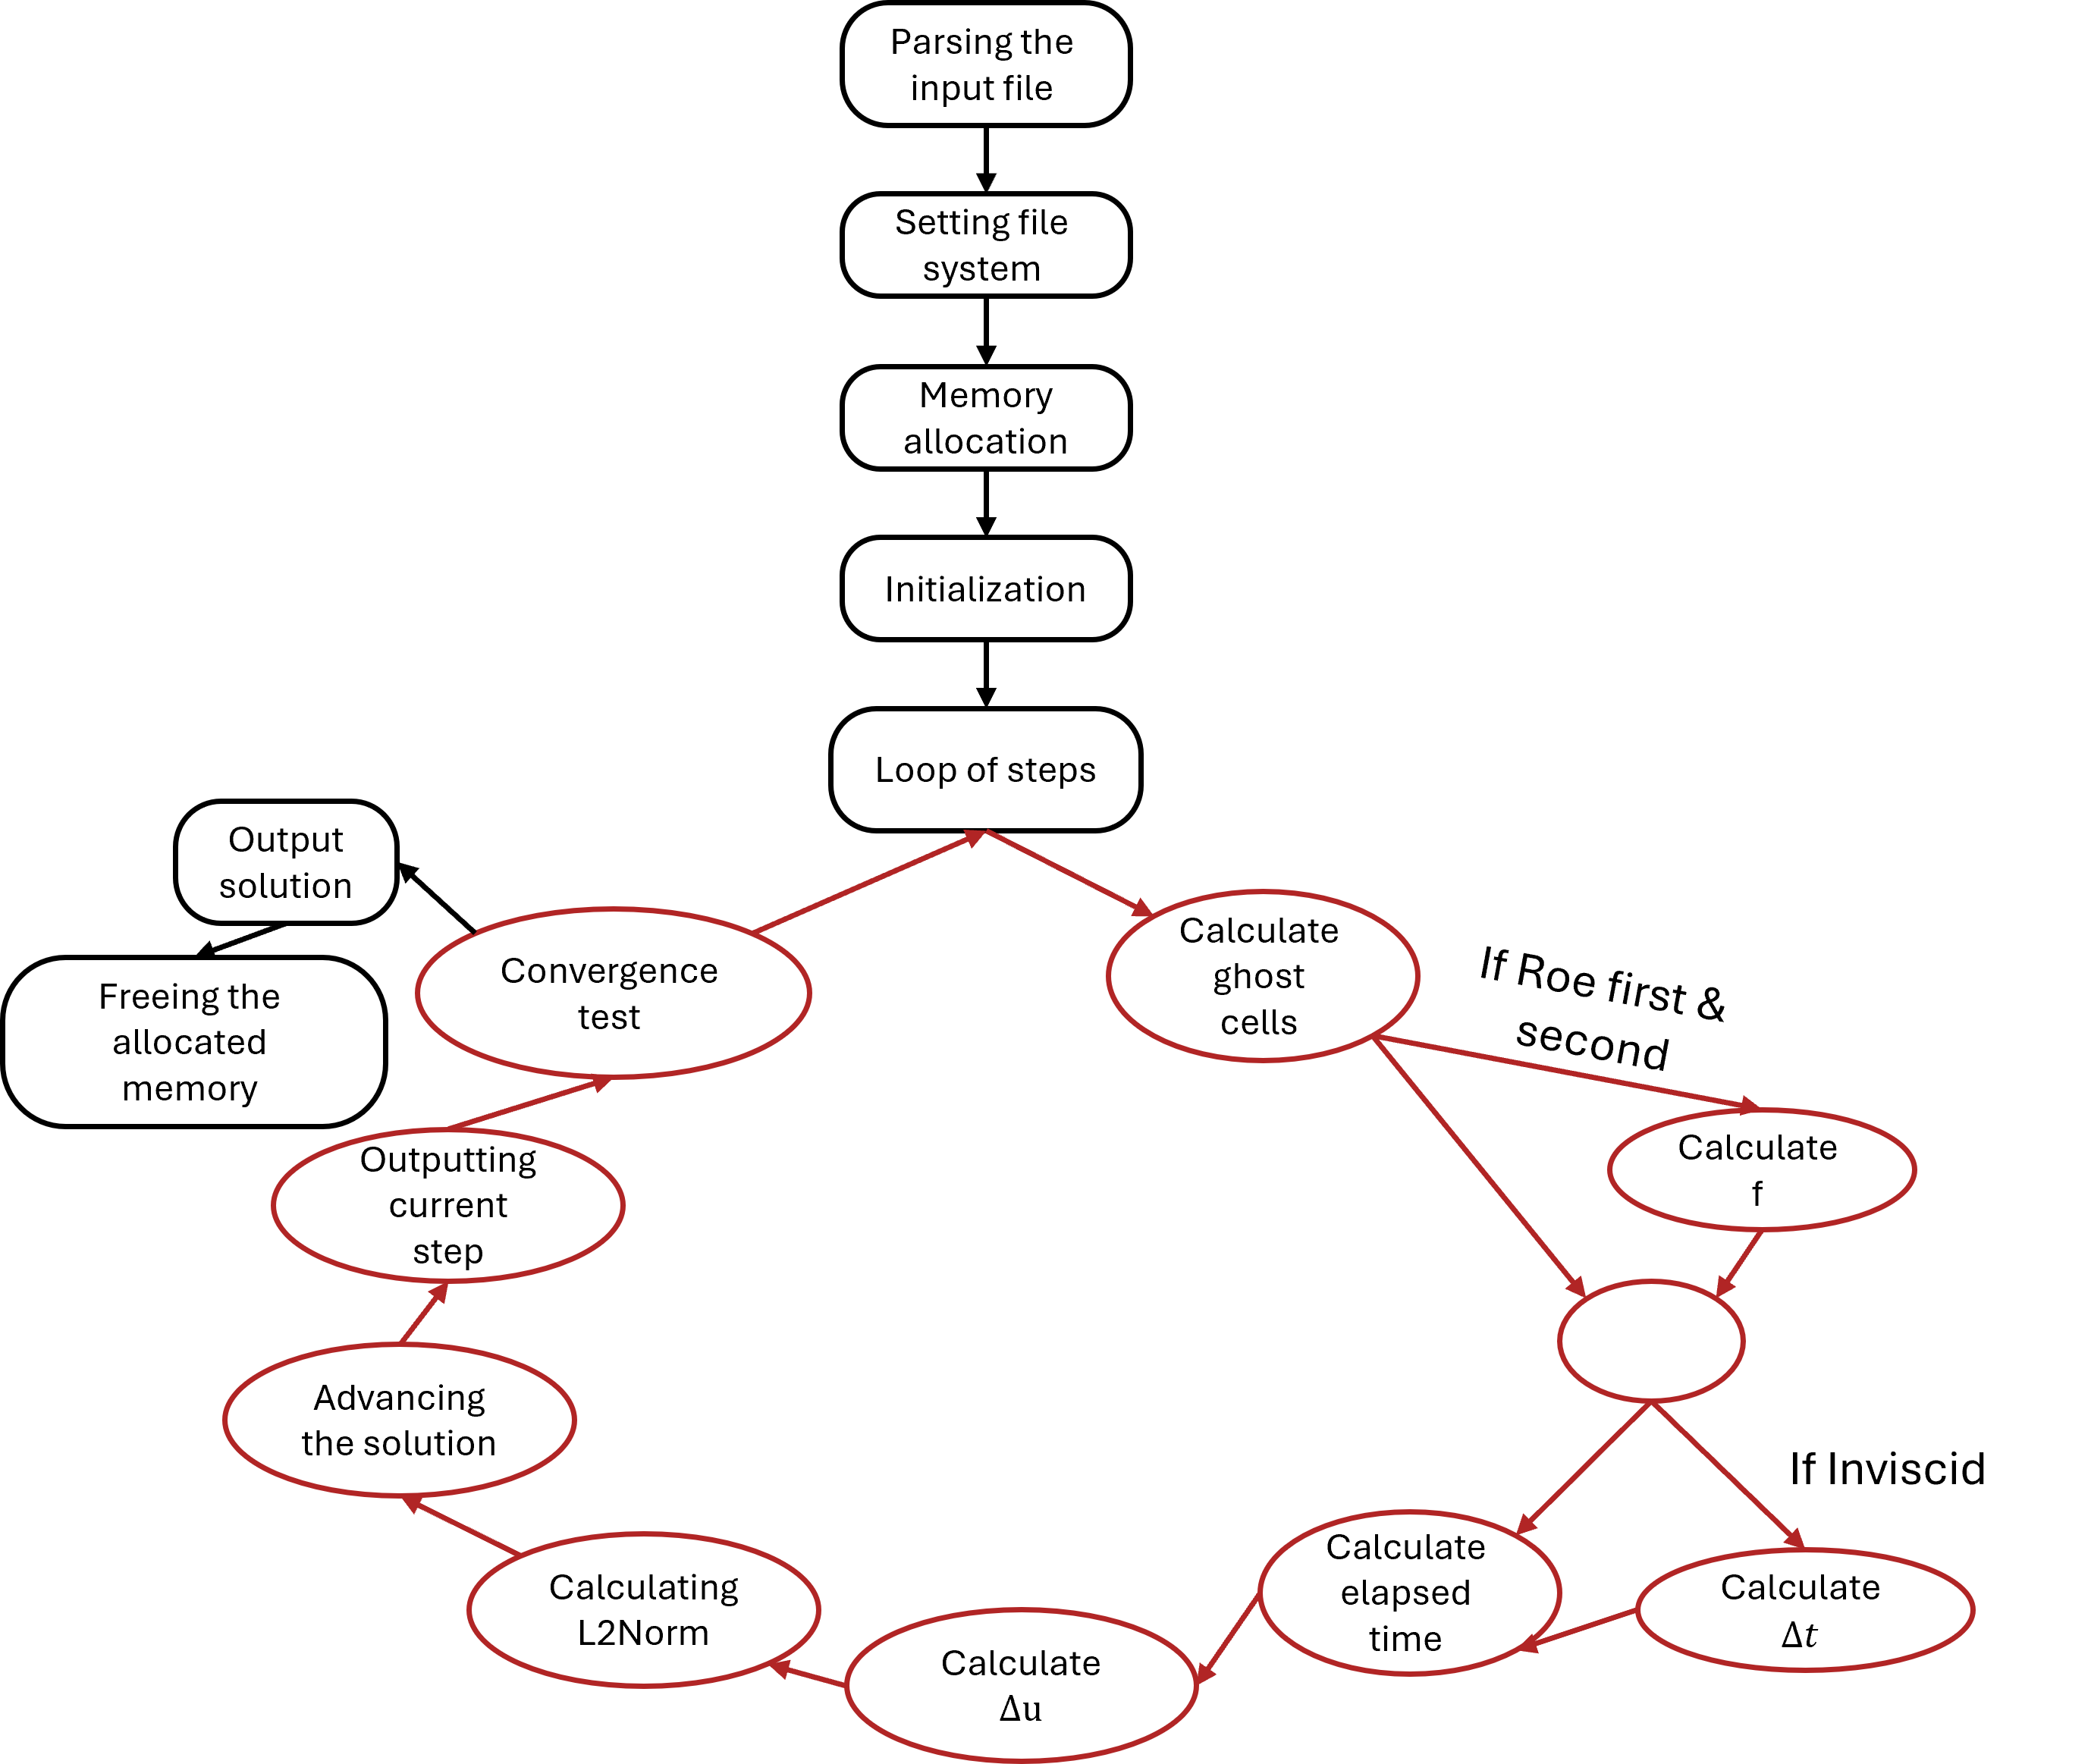
\includegraphics[width=\textwidth]{images/flow char.png}
    \caption{Flow Chart of the program}
    \label{fig:flow_chart}
\end{figure}
\subsection{The Functions in the Program}
The functions that are included in the program and explanations about them are included in the code itself.


\end{document}